\documentclass[twoside]{book}
\usepackage{lectures}
\hypersetup{pdftitle={Differential geometry of curves and surfaces: a working approach},
pdfauthor={Anton Petrunin and Sergio Zamora Barrera}}
\makeindex

\begin{document}
\title{\tt Differential geometry\\ of curves and surfaces:\\ a working approach}
\author{\tt Anton Petrunin and Sergio Zamora Barrera}
\date{}
\maketitle
\thispagestyle{empty}


\chapter*{Preface}

These notes might be good for you if you plan to do differential geometry,
or if you want to have a solid ground not to do it in the future.

Differential geometry does geometry on top of several branches of mathematics including 
real analysis, 
measure theory,
calculus of variation,
differential equations,
elementary and convex geometry,
topology, and more.
This subject is wide even at the entrance. 
By that reason it is fun and pain to teach and to study.

We discuss smooth curves and surfaces --- the main gate to differential geometry.
This subject provides a collection of examples and ideas critical for further study.
It is wise to become a master in this subject before making further steps --- no need for a rush.

We give an idea about subject, keeping it elementary, visual, and virtually rigorous; we allow gaps that belong to other branches of mathematics (these subjects discussed briefly in the appendixes).

We try to minimize the distance between definitions and meaningful results.
The highest points in these notes are
the theorem of Vladimir Ionin and Herman Pestov about closed curves with bounded curvature,
the theorem of Sergei Bernstein's on saddle graphs,
and the theorem of Stephan Cohn-Vossen on existence of simple two-sided infinite geodesic on an open convex surface.
These theorems give the first nontrivial examples of the so called \emph{local to global theorems} --- the hart of differential geometry. 

These notes are based on lectures at MASS program (Mathematics Advanced Study Semesters at Pennsylvania State University) Fall semester 2018.
Number of these topics were presented on the lectures of Yurii Burago who was teaching the first author at the Leningrad University.

An excellent minimalist introductory textbook with a more classical approach was written by Aleksei Chernavskii \cite{chernavsky};
if you read Russian, use it as a complementary source for this course. 
For a deeper diving into the subject we recommend the textbook of Victor Toponogov~\cite{toponogov}.

\part{Preliminaries}
\addtocounter{chapter}{-1}
\chapter{Preliminaries}

The chapter should be used as a quick reference when reading the book;
it also contain all necessary references with complete proof.

The fist section on metric spaces is most important;
we suggest to read in before going further.

\section{Metric spaces}\label{sec:metric-spcaes}

We assume that the reader is familiar with the notion of metric in 
Euclidean space.
In this chapter briefly discuss its generalization and fix notations that will be used further.

\subsection*{Definitions}

\emph{Metric} is a function that returns a real value $\Dist(x,y)$ for any pair $x,y$ in a given nonempty set $\mathcal X$  and satisfies the following axioms for any triple $x,y,z$: \label{page:def:metric}
\begin{enumerate}[(a)]
\item\label{def:metric-space:a} Positiveness: 
$$\Dist(x,y)\ge 0.$$
\item\label{def:metric-space:b} $x=y$ if and only if 
$$\Dist(x,y)=0.$$
\item\label{def:metric-space:c} Symmetry: $$\Dist(x, y) = \Dist(y, x).$$
\item\label{def:metric-space:d} Triangle inequality: 
$$\Dist(x, z) \le \Dist(x, y) + \Dist(y, z).$$
\end{enumerate}\

A set with a metric is called \index{metric space}\emph{metric space} and the elements of the set are called \index{point}\emph{points}.

\subsection*{Shortcut for distance}
Usually we consider only one metric on a set, therefore we can denote the metric space and its underlying set by the same letter, say $\mathcal X$.
In this case we also use a shortcut notations $|x-y|$ or $|x-y|_\mathcal X$ for the {}\emph{distance $\Dist(x,y)$ from $x$ to $y$ in $\mathcal X$}.
For example, the triangle inequality can be written as 
$$|x-z|_{\mathcal X}\le |x-y|_{\mathcal X}+|y-z|_{\mathcal X}.$$

\subsection*{Examples}
Euclidean space and plane as well as real line will be the most important examples of metric spaces for us.
In these examples the introduced notation $|x-y|$ for the distance from $x$ to $y$ has perfect sense as a norm of the vector $x-y$.
However, in general metric space the expression $x-y$ has no sense, but anyway we use expression $|x-y|$ for the distance.

Usually, if we say {}\emph{plane} or {}\emph{space} we mean {}\emph{Eucledean} plane or space.
However the plane (as well as the space) admits many other metrics, for example the so-called \index{Manhattan metric}\emph{Manhattan metric} from the following exercise.

\begin{thm}{Exercise}\label{ex:ell-infty}
Consider the function
$$\Dist(p,q)=|x_1-x_2|+|y_1-y_2|,$$
where $p=(x_1,y_1)$ and $q=(x_2,y_2)$ are points in the coordinate plane $\RR^2$.
Show that $\Dist$ is a metric on $\RR^2$.
\end{thm}

Let us mention another example: the \index{discrete space}\emph{discrete space} --- arbitrary nonempty set $\mathcal X$ with the metric defined as $|x\z-y|_{\mathcal X}=0$ if $x=y$ and $|x-y|_{\mathcal X}=1$ otherwise.

\subsection*{Subspaces}
Any subset of a metric space is also a metric space, by restricting the original metric to the subset;
the obtained metric space is called a \index{subspace of metric space}\emph{subspace}.
In particular, all subsets of Euclidean space are metric spaces.

\subsection*{Balls}
Given a point $p$ in a metric space ${\mathcal X}$ and a real number $R\ge 0$, the set of points $x$ on the distance less then $R$ (at most $R$) from $p$ is called \index{open ball}\emph{open} (respectively \index{closed ball}\emph{closed}) \emph{ball} of radius $R$ with center at $p$.
The {}\emph{open ball} is denoted as $B(p,R)$ or $B(p,R)_{\mathcal X}$;
the second notation is used if we need to emphasize that the ball lies in the metric space $\mathcal X$.
Formally speaking
\[B(p,R)=B(p,R)_{\mathcal X}=\set{x\in \mathcal X}{|x-p|_{\mathcal X}< R}.\]
Analogously, the {}\emph{closed ball} is denoted as $\bar B[p,R]$ or $\bar B[p,R]_{\mathcal X}$ and
\[\bar B[p,R]=\bar B[p,R]_{\mathcal X}=\set{x\in \mathcal X}{|x-p|_{\mathcal X}\le R}.\]

\begin{thm}{Exercise}\label{ex:B2inB1}
Let $\mathcal X$ be a metric space.

\begin{subthm}{ex:B2inB1:a} Show that if $\bar B[p,2]\subset \bar B[q,1]$ for some points $p,q\in \mathcal X$, then $\bar B[p,2]= \bar B[q,1]$.
\end{subthm}

\begin{subthm}{ex:B2inB1:b} Construct a metric space $\mathcal X$ with two points $p$ and $q$ such that the strict inclusion
$B(p,\tfrac32)\subset B(q,1)$ holds.
\end{subthm}

\end{thm}



\subsection*{Continuity}

In this section we will extend standard notions from calculus to the metric spaces.

\begin{thm}{Definition}
 Let ${\mathcal X}$ be a metric space.
A sequence of points $x_1, x_2, \ldots$ in ${\mathcal X}$ is called \index{convergent sequence of points}\emph{convergent}
if there is 
$x_\infty\in {\mathcal X}$ such that $|x_\infty -x_n|\to 0$ as $n\to\infty$.  
That is, for every $\eps > 0$, there is a natural number $N$ such that for all $n \ge N$, we have
\[|x_\infty-x_n|_{\mathcal X} < \eps.\]

In this case we say that the sequence $(x_n)$ {}\emph{converges} to $x_\infty$, 
or $x_\infty$ is the {}\emph{limit} of the sequence $(x_n)$.
Notationally, we write $x_n\to x_\infty$ as $n\to\infty$
or $x_\infty=\lim_{n\to\infty} x_n$.
\end{thm}

\begin{thm}{Definition}\label{def:continous}
Let ${\mathcal X}$ and ${\mathcal Y}$ be metric spaces.
A map $f\:{\mathcal X}\to {\mathcal Y}$ is called \index{continuous function}\index{continuous map}\emph{continuous} if for any convergent sequence $x_n\to x_\infty$ in ${\mathcal X}$,
%the sequence $y_n\z=f(x_n)$ converges to $y_\infty=f(x_\infty)$ in ${\mathcal Y}$.
we have $f(x_n) \to f(x_\infty)$ in ${\mathcal Y}$.

Equivalently, $f\:{\mathcal X}\to {\mathcal Y}$ is continuous if for any $x\in {\mathcal X}$ and any $\eps>0$,
there is $\delta>0$ such that 
$$|x-x'|_{\mathcal X}<\delta\ \text{ implies }\ |f(x)-f(x')|_{\mathcal Y}<\eps.$$
%$$|x-x'|_{\mathcal X}<\delta\ \Rightarrow\ |f(x)-f(x')|_{\mathcal Y}<\eps.$$

\end{thm}

\begin{thm}{Exercise}\label{ex:shrt=>continuous}
Let ${\mathcal X}$ and ${\mathcal Y}$ be metric spaces $f\:{\mathcal X}\to {\mathcal Y}$ is \index{distance non-expanding map}\emph{distance non-expanding map}; that is, 
\[|f(x)-f(x')|_{\mathcal Y}\le |x-x'|_{\mathcal X}\]
for any $x,x'\in \mathcal X$.
Show that $f$ is continuous.
\end{thm}

\begin{thm}{Definition}
Let ${\mathcal X}$ and ${\mathcal Y}$ be metric spaces.
A continous bijection $f\:{\mathcal X}\to {\mathcal Y}$ 
is called a \index{homeomorphism}\emph{homeomorphism} 
if its inverse $f^{-1}\:{\mathcal Y}\z\to {\mathcal X}$ is also continuous.

If there exists a homeomorphism $f\:{\mathcal X}\to {\mathcal Y}$,
we say that ${\mathcal X}$ is {}\emph{homeomorphic} to ${\mathcal Y}$,
or  $\mathcal X$ and ${\mathcal Y}$ are {}\emph{homeomorphic}.
\end{thm}

If a metric space $\mathcal X$ is homeomorphic to a known space, for example plane, sphere, disc, circle and so on,
we may also say that $\mathcal X$ is a \index{topological}\emph{topological} plane, sphere, disc, circle and so on.

\begin{thm}{Definition}
A subset $A$ of a metric space $\mathcal{X}$ is called \index{closed set}\emph{closed} if whenever a sequence $(x_n)$ of points from $A$ converges in $\mathcal{X}$, we have that $\lim_{n\to\infty} x_n \in A$.

A set $\Omega \subset \mathcal{X}$ is called \index{open set}\emph{open} if for any $z\in \Omega$, 
there is $\eps>0$ such that $B(z,\eps)\subset\Omega$.
\end{thm}

An open set $\Omega$ that contains a given point $p$ is called \index{neighborhood}\emph{neighborhood of $p$}.

\begin{thm}{Exercise}\label{ex:close-open}
Let $Q$ be a subset of a metric space $\mathcal{X}$.
Show that $Q$ is closed if and only if its complement $\Omega=\mathcal{X}\backslash Q$ is open.
\end{thm}

\chapter{Multivariable calculus}

\section{Regular values}

A map $\bm{f}\:\RR^n\to\RR^k$ can be thought as an array of functions 
\[f_1,\dots,f_k\:\RR^n\to \RR.\]
The map $\bm{f}$ is called \emph{smooth} if each function $f_i$ is smooth;
that is, all partial derivatives of $f_i$ are defined in the domain of definition of $\bm{f}$.

The following matrix
\[\Jac_{\bm{x}}\bm{f}=
\begin{pmatrix}
\dfrac{\partial f_1}{\partial x_1} & \cdots & \dfrac{\partial f_1}{\partial x_n}\\
\vdots & \ddots & \vdots\\
\dfrac{\partial f_k}{\partial x_1} & \cdots & \dfrac{\partial f_k}{\partial x_n} \end{pmatrix}\]
is called \emph{Jacobian matrix} of $\bm{f}$; we assume that the right hand side is evaluated at $\bm{x}=(x_1,\dots,x_n)$.

Inverse function theorem gives a sufficient condition for a smooth function to be invertible in a neighborhood of a given point $p$ in its domain.
The condition is formulated in terms of the partial derivatives of $f_i$ at $p$.

Implicit function theorem is a close relative to inverse function theorem;
in fact it can be obtained as its corollary.
It is used for instance when we need to pass from parametric to implicit description of curves and surfaces.

Both theorems reduce the existence of a map satisfying certain equation to a question in linear algebra that can be written in terms of its Jacobian matrix.
We use these two theorems only for $n\le 3$.

These two theorems are discussed in any course of multivariable calculus, the classical book of Walter Rudin \cite{rudin} is one of my favorites.

\begin{thm}{Inverse function theorem}\label{thm:inverse}
Let $\bm{f}=(f_1,\dots,f_n)\:\RR^n\to\RR^n$ be a smooth map.
Assume that the Jacobian matrix
\[
\begin{pmatrix}
\dfrac{\partial f_1}{\partial x_1} & \cdots & \dfrac{\partial f_1}{\partial x_n}\\
\vdots & \ddots & \vdots\\
\dfrac{\partial f_n}{\partial x_1} & \cdots & \dfrac{\partial f_n}{\partial x_n} \end{pmatrix}\]
is invertible at some point $p$ in the domain of definition of $\bm{f}$.
Then there is a smooth function $\bm{h}\:\RR^m\to\RR^n$ defined in a neighborhood $\Omega_q$ of $q=\bm{f}(p)$ that is a \emph{local inverse of $\bm{f}$ at $p$};
that is, there is a neighborhood $\Omega_p\ni p$ such that
$\bm{f}$ defines a bijection $\Omega_p\to \Omega_q$ and
$\bm(h) \circ \bm{f}(x)=x$ for any $x\in \Omega_p$.
\end{thm}

\begin{thm}{Implicit function theorem}\label{thm:imlicit}
Let $\bm{f}=(f_1,\dots,f_n)\:\RR^{n+m}\to\RR^n$ be a smooth map,
$m,n\ge 1$.
Let us consider $\RR^{n+m}$ as a product space $\RR^n\times \RR^m$ with coodinates 
$x_1,\dots,x_n,y_1,\dots,y_m$.
Consider the following matrix 
\[
M=\begin{pmatrix}
\dfrac{\partial f_1}{\partial x_1} & \cdots & \dfrac{\partial f_1}{\partial x_n}\\
\vdots & \ddots & \vdots\\
\dfrac{\partial f_n}{\partial x_1} & \cdots & \dfrac{\partial f_n}{\partial x_n} \end{pmatrix}\]
formed by the first $n$ columns of the Jacobian matrix.
Assume $M$ is invertible at some point $p$ in the domain of definition of $\bm{f}$ and $\bm{f}(p)=0$.
Then there is a neighborhood $\Omega_p\ni p$
and a smooth function $\bm{h}\:\RR^m\to\RR^n$ defined in a neighborhood $\Omega_0\ni 0$ such that
for any $(x_1,\dots,x_n,y_1,\dots y_m)\in \Omega_p$, the equality
\[\bm{f}(x_1,\dots,x_n,y_1,\dots y_m)=0\]
holds if and only if 
\[(x_1,\dots x_n)=\bm{h}(y_1,\dots y_m).\]

\end{thm}

If the assumption in the theorem holds for any point $p$ such that $\bm{f}(p)=0$,
then we say that $0$ is a regular value of $\bm{f}$.
The following lemma states that most values of a smooth map are regular;
in particular, generic smooth functions satisfy the assumption of the theorem.

\begin{thm}{Sard's lemma}\label{lem:sard}
Given a smooth map $\bm{f}\colon U \z\to \RR^m$ defined on an open set $U\subset \RR^n$, most of the values in $\RR^m$ are regular.
\end{thm}

The words \emph{almost all} means all values, with the possible exception of a set of zero Lebesgue measure.
In particular if one chooses a random value equidistributed in an arbitrarily small ball $B\subset \RR^m$, then it is a regular value of $f$ with probability 1.


\section{Multiple integral}

The following theorem is a substitution rule for multiple variables.

\begin{thm}{Theorem}\label{thm:mult-substitution}
Let $K\subset \RR^n$ be a compact set and $h\:K\to\RR$ be a bounded measurable function.
Assume $\bm{f}\:K\to \RR^n$ is an injective smooth map.
Then 
\[\int_K h(\bm{x})\cdot |\Jac_{\bm{x}}\bm{f}|\cdot d\bm{x}
=
\int_{\bm{f}(K)} h\circ \bm{f}^{-1}(\bm{y})\cdot d\bm{y},\]
where $J_{\bm{f}}(\bm{x})$ denotes the Jacobian of $\bm{f}$ at $\bm{x}$;
that is, the determinant of the Jacobian matrix of $\bm{f}$ at $\bm{x}$.

\end{thm}


\begin{thm}{Area formula}\label{thm:area-formula}
Let $\bm{f}\:K\to\RR^n$ be a smooth map defined on a compact set $K\subset \RR^n$;
denote by $J_{\bm{f}}$ the Jacobian of $\bm{f}$.
Then for any function $h\:K\to \RR$
\[\int_K h(\bm{x})\cdot |\Jac_{\bm{x}}\bm{f}|\cdot d\bm{x}=\int_{\bm{f}(K)} H_K(\bm{y})\cdot d\bm{y},\]
where 
\[H_K(\bm{y})=\sum_{\substack{\bm{x}\in K \\ \bm{f}(\bm{x})=\bm{y}}}h(\bm{x}).\]
(The integrals are understood in the sense of Lebesgue.)
\end{thm}

Let us sketch the proof of area formula using  Sard's lemma (\ref{lem:sard}) and the substitution rule (\ref{thm:mult-substitution}).

\parit{Sketch of proof.}
Denote by $S\subset K$ the set of critical points of $\bm{f}$; that is, $\bm{x}\in S$ if $J_{\bm{f}}(\bm{x})=0$.
By Sard's lemma,
\emph{$\bm{f}(S)$ has vanishing measure}.
Note that 
\[\int_S h(\bm{x})\cdot |J_{\bm{f}}(\bm{x})|\cdot d\bm{x}=0\]
since $J_{\bm{f}}(\bm{x})=0$
and
\[\int_{\bm{f}(S)} H_S(\bm{y})\cdot d\bm{y}\]
since $\bm{f}(S)$ has vanishing measure.
In particular,
\[\int_S h(\bm{x})\cdot |J_{\bm{f}}(\bm{x})|\cdot d\bm{x}=\int_{\bm{f}(S)} H_S(\bm{y})\cdot d\bm{y};\]
that is the area formula holds for $S$.

It remains to prove that 
\[\int_{K\backslash S} h(\bm{x})\cdot |J_{\bm{f}}(\bm{x})|\cdot d\bm{x}=\int_{\bm{f}(K\backslash S)} H_{K\backslash S}(\bm{y})\cdot d\bm{y}.\]
Since $J_{\bm{f}}(\bm{x})\ne 0$ for any $\bm{x}\in K\backslash S$, by inverse function theorem, the restriction of $\bm{f}$ to a neighborhood $U\ni\bm{x}$ has a smooth inverse.
Therefore for any compact set $K'\subset U$ we have that %???compact
\[\int_{K'}h(\bm{x})\cdot |J_{\bm{f}}(\bm{x})|\cdot d\bm{x}=\int_{\bm{f}(K_1)} h(\bm{f}^{-1}(\bm{y}))\cdot d\bm{y}.\]
It remains to subdivide $K_1$ into a countable collection of subsets of that type and sum up the corresponding formulas.\qeds

\section{Divergence theorem}

\begin{thm}{Theorem}\label{thm:div}
If a piecewise smooth surface $\Sigma$ bounds a body $V$ in $\RR^3$, then
\[\flux_{\vec u}\Sigma=\iiint_V\div \vec u,\]
assuming that the orientation on $\Sigma$ is defined by a unit normal field that points out of $V$.
\end{thm}


\section{Curl theorem}

\begin{thm}{Theorem}\label{thm:curl}
???
\end{thm}



\chapter{Differential equations}

\section{Initial value problem}

The following theorem guarantees existence and uniqueness of solutions of an initial value problem
for a system of ordinary differential equations
\[
\begin{cases}
x_1'(t)&=f_1(x_1,\dots,x_n,t),
\\
&\dots
\\
x_n'(t)&=f_n(x_1,\dots,x_n,t),
\end{cases}
\]
where each $x_i=x_i(t)$ is a real valued function defined on a real interval $\mathbb{I}$
and each $f_i$ is a smooth function defined on $\RR^n\times \mathbb{I}$.

The array of functions $(f_1,\dots,f_n)$ can be considered as one vector-valued function 
$\bm{f}\:\RR^n\times \mathbb{I}\to \RR^n$ and the array $(x_1,\dots,x_n)$ can be considered as a vector  $\bm{x}\in\RR^n$.
Therefore the system can be rewritten as one vector equation 
\[\bm{x}'(t)=\bm{f}(\bm{x}, t).\] 

%??? make it for arbitrary domain
%??? higher order
\begin{thm}{Theorem}\label{thm:ODE}
Suppose $\mathbb{I}$ is a real interval and $\bm{f}\:\RR^n\times\mathbb{I}\to \RR^n$ is a smooth function.
Then for any initial data $\bm{x}(t_0)=\bm{u}$ the differential equation 
\[\bm{x}'(t)=\bm{f}(\bm{x},t)\]
has a unique solution $\bm{x}(t)$ defined at a maximal subinterval $\mathbb{J}$ of $\mathbb{I}$ that contains $t_0$.
Moreover
\begin{enumerate}[(a)]
\item  if $\mathbb{J}\ne \mathbb{I}$ (that is, if an end $a$ of $\mathbb{J}$ lies in the interior of $\mathbb{I}$) then $\bm{x}(t)$ diverges as $t\to a$;
\item  the function $(\bm{u},t_0,t)\mapsto \bm{x}(t)$ is smooth.
\end{enumerate}


\end{thm}

\chapter{Real analysis}

\section{Lipschitz condition}

Recall that a function $f$ between metric spaces is called Lipschitz if there is a constant $L$ such that 
\[|f(x)-f(y)|\le L\cdot|x-y|\]
for all values $x$ and $y$ in the domain of definition of $f$.
%Although this definition makes sense for maps between metric spaces, we will only use it for real-to-real functions.

\begin{thm}{Rademacher's theorem}\label{thm:rademacher}
Let $f\:[a,b]\to\RR$ be a Lipschitz function.
Then the derivative $f'(x)$ is defined for alomst all $x\in [a,b]$.
Moreover the derivative $f'$ is a bounded measurable function defined almost everywhere in $[a,b]$ and it satisfies the fundamental theorem of calculus; that is, the following identity 
\[f(b)-f(a)=\int_a^b f'(x)\cdot dx,\]
holds if the integral is understood in the sense of Lebesgue.
\end{thm}

The following theorem makes possible to extend many statements about continuous function to measurable functions.

\begin{thm}{Lusin's theorem}\label{thm:lusin}
Let $\phi\:[a,b]\to \RR$ be a measurable function.
Then for any $\eps>0$, there is a continuous function $\psi_\eps\:[a,b]\to \RR$ that coincides with $\phi$ outside of a set of measure at most $\eps$.
Moreover, if $\phi$ is bounded above and/or below by some constants, then we may assume that so is $\psi_\eps$.  
\end{thm}

\section{Uniform continuity and convergence}

Let $f$ be a real function defined on a real interval.
If  for any $\eps>0$ there is $\delta>0$ such that 
\[|x_1-x_2|_X<\delta\quad\Longrightarrow\quad |f(x_1)-f(x_2)|_Y<\eps,\]
then $f$ is called \emph{uniformly continuous}.

Evidently every uniformly continuous function is continuous;
the converse does not hold.
For example, the function $f(x)=x^2$ is continuous, but not uniformly continuous.

However if $f$ is continuous and defined on a closed interval $[a,b]$, then $f$ is uniformly continuous

If the condition above holds for any function $f_n$ in a sequence and $\delta$ depend solely on $\eps$,
then the sequence $(f_n)$ is called uniformly equicontinuous.
More precisely, 
a sequence of functions $f_n:X\to Y$ is called \emph{uniformly equicontinuous} if 
for any $\eps>0$ there is $\delta>0$ such that 
\[|x_1-x_2|_X<\delta\quad\Longrightarrow\quad |f_n(x_1)-f_n(x_2)|_Y<\eps\]
for any $n$.
Uniform equicontinuity is the condition in one of the most important convergence theorems in analysis. 
We say that a sequence of functions $f_i : X \to Y$ converges uniformly to a function $f_{\infty}: X \to Y$ if for any 
$\varepsilon >0$, there is a natural number $N$ such that for all $n \geq N$, we have $| f_{\infty} (x)- f_n (x) | < \varepsilon$
for all $x  \in X$.

\begin{thm}{Arzel\'{a}-Ascoli Theorem}\label{lem:equicontinuous}
Any uniformly equicontinuous sequence of function $f_n\:[a,b]\to [c,d]$ has a subsequence that converges uniformly to a continuous function. 
\end{thm}

\chapter{Topology}

\section{Jordan's theorem}

We sometimes use the following characterization of homeomorphisms between compact spaces.

\begin{thm}{Theorem}\label{thm:Hausdorff-compact}
A continuous bijection $f$ between compact metric spaces has a continuous inverse;
that is, $f$ is a homeomorphism.
\end{thm}


The first part of the following theorem was proved by Camille Jordan, the second part is due to Arthur Schoenflies.

\begin{thm}{Theorem}\label{thm:jordan}
The complement of any closed simple plane curve $\gamma$ has exactly two connected components. 

Moreove, there is a homeomorphism $h\:\RR^2\to \RR^2$ that maps the unit circle to $\gamma$.
In particular $\gamma$ bounds a topological disc.
\end{thm}

This theorem is known for its simple formulation and quite hard proof.
By now many proofs of this theorem are known.
For the first statement, a very short proof based on a somewhat developed technique is given by Patrick Doyle \cite{doyle},
among elementary proofs, one of my favorites is the proof given by Aleksei Filippov \cite{filippov}.

We use the following smooth analog of this theorem.

\begin{thm}{Theorem}
The complement of any closed simple smooth regular plane curve $\gamma$ has exactly two connected components. 

Moreover the there is a diffeomorphism $h\:\RR^2\to \RR^2$ that maps the unit circle to $\gamma$.
\end{thm}

The proof of this statement is much simpler.
An amusing proof can be found in \cite{chambers-liokumovich}.

\section{Connectedness}

Recall that a continuous map $\alpha$ from the unit interval $[0,1]$ to a metric space is called a \emph{path}. If $p=\alpha (0)$ and $q = \alpha (1)$, then we say that $\alpha$ connects $p$ to $q$.


A set $X$ in the Euclidean space is called \emph{path connected} if any two points $x,y\in X$ can be connected by a path lying in $X$.

A set $X$ in the Euclidean space is called \emph{connected} if one cannot cover $X$ with two disjoint open sets $V$ and $W$ such that both intersections $X\cap V$ and $X\cap W$ are nonempty.

\begin{thm}{Proposition}
Any path connected set is connected.
Moreover, any open connected set in the Euclidean space or  plane is path connected.
\end{thm}

Given a point $x\in X$, the maximal connected subset of $X$ containing $x$ is called the \emph{connected component} of $x$ in $X$.



\chapter{Elementary geometry}

\begin{thm}{Theorem}\label{thm:sum=(n-2)pi}
The sum of all the internal angles of a simple $n$-gon is $(n-2)\cdot\pi$. 
\end{thm}


\parit{Proof.}
The proof is by induction on $n$.
For $n=3$ it says that sum of internal angles of a triangle is $\pi$, which is assumed to be known.

First let us show that for any $n\ge4$, any $n$-gon has a diagonal that lies inside of it.
Assume this holds true for all polygons with at most $n-1$ vertices.

Fix an $n$-gon $P$, $n\ge4$.
Applying a rotation if necessary, we can assume that all its vertexes have different $x$-coordinates.
Let $v$ be a vertex of $P$ that minimizes the $x$-coordinate;
denote by $u$ and $w$ its adjacent vertexes.
Let us choose the diagonal $uw$ if it lies in $P$.
Otherwise the triangle $\triangle uvw$ contains another vertex of $P$.
Choose a vertex $s$ in the interior of $\triangle uvw$ that maximizes the distance to line $uw$.
Note that the diagonal $vs$ lies in $P$;
if it is not the case, then $vs$ crosses another side $pq$ of $P$, one of the vertices $p$ or $q$ has larger distance to the line and it lies in the interior of $\triangle uvw$ --- a contradiction.

Note that the diagonal divides $P$ into two polygons, say $Q$ and $R$, with smaller number of sides in each, say $k$ and $m$ correspondingly.
Note that 
\[k+m=n+2;
\eqlbl{eq:k+m=n+2}\]
indeed each side of $P$ appears once as a side of $P$ or $Q$ plus the diagonal appears twice --- once as a side in $Q$ and once as a side of $R$.
Note that the sum of the angles of $P$ is the sum of the angles of $Q$ and $R$, which by the induction hypothesis are $(k-2)\cdot\pi$ and $(m-2)\cdot\pi$ correspondingly.
It remains to note that \ref{eq:k+m=n+2} implies
\[(k-2)\cdot\pi+(m-2)\cdot\pi=(n-2)\cdot\pi.\]
\qedsf

\section{Triangle inequality for angles}

The following theorem says that the triangle inequality holds for angles between half-lines from a fixed point.
In particular it implies that a sphere with the angle metric is a metric space.

\begin{thm}{Theorem}\label{thm:spherical-triangle-inq}
The inequality
\[\measuredangle aob+\measuredangle boc\ge\measuredangle aoc\]
holds for any three half-lines $oa$, $ob$ and $oc$ in the Euclidean space.
\end{thm}

The following lemma says that the angle of a triangle monotonically depends on the opposit side, assuming the we keep the other two sides fixed. It follows directly from the cosine rule.

\begin{thm}{Lemma}\label{lem:angle-monotonicity}
Let $x$, $y$, $z$, $x'$, $y'$ and $z'$ be 6 points such that $|x-y|=|x'-y'|>0$ and $|y-z|=|y'-z'|>0$.
Then 
\[\measuredangle xyz\ge \measuredangle x'y'z'
\quad\text{if and only if}\quad
|x-z|\ge |x'-z'|.\]
\end{thm}

\begin{wrapfigure}{o}{30 mm}
\vskip-0mm
\centering
\includegraphics{mppics/pic-69}
\vskip0mm
\end{wrapfigure}

\parit{Proof of \ref{thm:spherical-triangle-inq}.}
We can assume that $\measuredangle aob<\measuredangle aoc$; otherwise the statement is evident.
In this case there is a half-line $ob'$ in the angle $aoc$ such that 
\[\measuredangle aob=\measuredangle aob',\]
so in particular we have that
\[\measuredangle aob'+\measuredangle b'oc=\measuredangle aoc.\]
Without loss of generality we can assume that  $|o-b|=|o-b'|$ and $b'$ lies on a line segment $ac$, so
\[|a-b'|+|b'-c|=|a-c|.\]

Then by the triangle inequality 
\[
\begin{aligned}
|a-b|+|b-c|&\ge |a-c|=
\\
&=|a-b'|+|b'-c|.
\end{aligned}
\eqlbl{eq:triangle-inq-abcb'}
\]

Note that in the triangles $aob$ and $aob'$ the side $ao$ is shared, so $\measuredangle aob\z=\measuredangle aob'$ and $|o-b|=|o-b'|$.
By side-angle-side congruence condition, we have that $\triangle aob\cong \triangle aob'$;
in particular $|a-b'|=|a-b|$.
Therefore from \ref{eq:triangle-inq-abcb'} we get 
\[|b-c|\ge |b'-c|.\]
Applying the angle monotonicity (\ref{lem:angle-monotonicity}) we obtain
\[\measuredangle boc\ge \measuredangle b'oc.\]
Whence
\begin{align*}
\measuredangle aob+\measuredangle boc
&\ge \measuredangle aob'+\measuredangle b'oc=
\\
&=\measuredangle aoc.
\end{align*}
\qedsf

\section{Convexity}

A set $X$ in the Euclidean space is called \emph{convex} if for any two points $x,y\in X$, any point $z$ between $x$ and $y$ lies in $X$.
It is called  \emph{strictly convex} if for any two points $x,y\in X$, any point $z$ between $x$ and $y$ lies in the interior of $X$.

From the definition, it is easy to see that the intersection of an arbitrary family of convex sets is convex. 
The intersection of all convex sets containing $X$ is called the \emph{convex hull} of $X$;
it is the minimal convex set containing the set $X$.

We will use the following corollary of the so called \emph{hyperplane separation theorem}:

\begin{thm}{Lemma}\label{lem:separation}
Let $K\subset \RR^3$ be a closed convex set.
Then for any point $p\notin K$ there is a plane $\Pi$ that separates $K$ from $p$;
that is, $K$ and $p$ lie on opposite open half-spaces separated by $\Pi$.
\end{thm}

A function of two variables $(x,y)\mapsto f(x,y)$ is called convex if 
its epigraph $z\ge f(x,y)$ is a convex set.
This is equivalent to the so-called \emph{Jensen's inequality}
\[f \left (t\cdot x_1 + (1-t)\cdot x_2 \right ) \leq t\cdot f(x_1)+ (1-t)\cdot f(x_2)\]
for $t\in[0,1]$.
If $f$ is smooth, then the condition is equivalent to the following inequality for the second directional derivative:
\[D^2_wf\ge 0\]
for any vector $w\ne 0$ in the $(x,y)$-plane.

\chapter{Area}

\section{Area of spherical triangle}

\begin{thm}{Lemma}\label{lem:area-spher-triangle}
Let $\Delta$ be a spherical triangle;
that is, $\Delta$ is the intersection of three closed half-spheres in the unit sphere $\SS^2$.
Then 
\[\area\Delta=\alpha+\beta+\gamma-\pi,\eqlbl{eq:area(Delta)}\]
where $\alpha$, $\beta$ and $\gamma$ are the angles of $\Delta$.
\end{thm}

The value $\alpha+\beta+\gamma-\pi$ is called \emph{excess} of the triangle $\Delta$.

\begin{wrapfigure}{o}{22 mm}
\vskip-0mm
\centering
\includegraphics{mppics/pic-43}
\vskip-0mm
\end{wrapfigure}

\parit{Proof.}
Recall that 
\[\area\SS^2=4\cdot\pi.\eqlbl{eq:area(S2)}\]

Note that the area of a spherical slice $S_\alpha$ between two meridians meeting at angle $\alpha$ is proportional to $\alpha$.
Since for $S_\pi$ is a half-sphere, from \ref{eq:area(S2)}, we get $\area S_\pi\z=2\cdot\pi$.
Therefore the coefficient is 2; that is,
\[\area S_\alpha=2\cdot \alpha.\eqlbl{eq:area(Sa)}\]

Extending the sides of $\Delta$ we get 6 slices: two $S_\alpha$, two $S_\beta$ and two $S_\gamma$ which cover most of the sphere once,
but the triangle $\Delta$ and its centrally symmetric copy $\Delta'$ are covered 3 times.
It follows that
\[2\cdot \area S_\alpha+2\cdot \area S_\beta+2\cdot \area S_\gamma
=\area\SS^2+4\cdot\area\Delta.\]
Substituting \ref{eq:area(S2)} and \ref{eq:area(Sa)} and simplifying, we get \ref{eq:area(Delta)}.
\qeds

\section{Schwarz's boot}\label{sec:schwarz-boot}

Recall that we defined length of curve as the exact upper bound on the length of inscribed polygonal lines.
It suggests to define area of a surface as a exact upper bound on the area of polyhedrons inscribed in the surface.

However as you will see from the following example, this idea fails badly even for cylindrical surface.
Namely, we will show that if we define the area as the least upper bound of areas of inscribed polyhedral surfaces, 
then the area of the lateral surface of the cylinder must be infinite.
The latter contradicts correct intuition that the area of this surface should be the product of the circumference of the base circle and the height of the cylinder.


\begin{wrapfigure}{r}{42 mm}
\centering
\includegraphics{asy/schwarz}
\end{wrapfigure}

Let us divide the cylinder into $m$ equal cylinders by planes parallel to its base.
This way we obtain $m+1$ circles on the lateral surface of a cylinder, including both bases.
Further, let us divide each of these circles into $n$ equal arcs in such a way that the dividing points 
of a circle will lie exactly above the midpoints of arcs on the circle under it.
Consider all triangles formed by a chord of such arc and line segments connecting the ends of the chord with the points right above and right below the mid point of its arc.
All the $2mn$ equal triangles form a polyhedral surface which is called Schwarz's boot.
A Schwarz's boot for $m=8$ and $n=6$ is shown on the diagram.

{

\begin{wrapfigure}{o}{40 mm}
\centering
\includegraphics{mppics/pic-87}
\end{wrapfigure}

Consider one of the triangle $abc$ which form the Schwarz's boot.
By construction, its base $ac$ lies in a horizontal plane and the projection $b'$ of $b$ on this plane bisects the arc $ac$.
Therefore the vertexes of the triangle $ab'c$ are the three consequent vertexes of a regular $2n$-gone inscribed in a unit circle.
Denote the triangle $ab'c$ by $s_n$; clearly it depends only on $n$ and the radius of the base.


Both triangles $abc$ and $ab'c$ are isosceles with shares base $ac$.
Note that the altitude $bp$ is larger than the altitude $b'p$.
Therefore
\begin{align*}
\area (\triangle abc)&=\tfrac12\cdot |a-c|\cdot |b-p|>
\\
&>\tfrac12\cdot |a-c|\cdot |b'-p|=
\\
&=\area (\triangle ab'c)=
\\
&=s_n.
\end{align*}

}

In particular,
\[S_{m,n}>2\cdot m\cdot n\cdot s_n,\]
where $S_{m,n}$ denotes the total area of the Schwarz's boot.
Consider the pairs $(m,n)$ such that $m$ is much larger than $n$; namely $m>\tfrac1{s_n}$.
Then
\[S_{m,n}> 2\cdot  m\cdot  n\cdot  s_n>2\cdot  \tfrac1{s_n}\cdot  n\cdot  s_n=2\cdot n.\]
Therefore $S_{m,n}\to \infty$ as $n\to \infty$.

\part{Curves}
\chapter{Curves}

\parbf{Paths.}
Let $\mathcal{X}$ be a metric space.
A continuous map $f\:[0,1]\to\mathcal{X}$ is called a \emph{path}.
If $p=f(0)$ and $q=f(1)$, then we say that \emph{$f$ connects $p$ to $q$}.

If any two points in $\mathcal{X}$ can be connected by a path then $\mathcal{X}$ is called \emph{path connected}.
Similarly, a subset $A\subset \mathcal{X}$ is called \emph{path connected} if any two points $p,q\in A$ can be connected by a path that runs in $A$;
equivalently, the subspace $A$ is path connected.

\parbf{Simple curves.}

\begin{thm}{Definition} 
A path connected subset $\gamma$ in a metric space is called a \emph{simple curve} if it is \emph{locally} homeomorphic to a real interval; that is, any point $p\in\gamma$ has a neighborhood $U\ni p$ such that the intersection
$U\cap \gamma$ is homeomorphic to a real interval.
\end{thm} %???change def

It turns out that any curve $\gamma$ admits a homeomorphism from a real interval or a circle;
that is, there is a continuous bijection $G\to \gamma$ with continuous inverse;
here (and further) $G$ denotes a circle or real interval.
We omit a proof of this statement, but it is not hard.

The homeomorphism $G\to \gamma$ as above is called \emph{parametrization} of~$\gamma$.
The parametrization completely defines the curve.
Often will use the same letter for curve and its parametrization, so we can say curve $\gamma$ has parametrization $\gamma\:G\to \mathcal{X}$.
Note however that any curve admits many different parametrization. 

\begin{thm}{Exercise}
Find a continuous injective map $\gamma\:[0,1)\to\RR^2$ such that its image is not a simple curve.
\end{thm}

\parit{Hint:} The image of $\gamma$ should have a shape of digit $9$.


If $G$ is a circle, then the curve $\gamma\:G\to \mathcal{X}$ is called \emph{closed}.
If $G$ is a real interval, then  we may say that $\gamma$ is an \emph{arc}.

\parbf{Parameterized curves.}
A \emph{parameterized curve} is defined as a continuous map $\gamma\: G\to \mathcal{X}$. 
For a parameterized curve we do not assume that $\gamma$ is injective; in other words the parameterized curve might have self-intersections.

\begin{thm}{Advanced exercise}
Let $\alpha\:[0,1]\to\mathcal{X}$ be a path from $p$ to $q$.
Assume $p\ne q$.
Show that there is a simple path connecting from $p$ to $q$ in~$\mathcal{X}$.
\end{thm}

\section*{Smooth curves}

A curve in the Euclidean space or plane, called \emph{space} or \emph{plane curve} correspondingly.

A space curve can be described by its coordinate functions 
\[\gamma(t)=(x(t),y(t),z(t)).\]
Plane curves can be considered as a partial case of space curves with $z(t)\equiv 0$.

If each of the coordinate functions $x(t),y(t),z(t)$ of the space curve $\gamma$ is a smooth (that is, it has derivatives of all orders everywhere in its domain) then the parameterized curve is called \emph{smooth}.

If the \emph{velocity vector} 
\[\gamma'(t)=(x'(t),y'(t),z'(t))\] 
does not vanish at all points, then the parameterized curve $\gamma$ is called \emph{regular}.

A simple space curve is called \emph{smooth and regular} if it admits a smooth and regular parametrization correspondingly.
Regular smooth curves are among the main objects in differential geometry;
the term \emph{smooth curve} often used for \emph{smooth regular curve}. 

\begin{thm}{Exercise}\label{ex:L-shape}
The function 
\[f(t)=
\begin{cases}
0&\text{if}\ t\le 0,
\\
\frac{t}{e^{1\!/\!t}}&\text{if}\ t> 0.
\end{cases}
\]
is smooth.\footnote{The existence of all derivatives $f^{(n)}(x)$ at $x\ne 0$ is evident and direct calculations show that $f^{(n)}(0)=0$ for any $n$.}

Show that $\gamma(t)=(f(t),f(-t))$ gives a smooth parametrization of the curve $S$ formed by the union of two half-axis in the plane.

Show that any smooth parametrization of $S$ has vanishing velocity vector at the origin.
Conclude that the curve $S$ is not regular and smooth.
\end{thm}


\begin{thm}{Exercise}\label{ex:cycloid}
Describe the set of real numbers $a$
such that the plane curve $\gamma_a(t)= (t+a\cdot \sin t,a\cdot \cos t)$, $t\in\RR$ is
\begin{enumerate}[(a)]
\item regular;
\item simple.
\end{enumerate}

\end{thm}

\parbf{Loops and periodic parametrization.}
A closed simple curve can be described as an image of a parameterized curve $\gamma\: [0,1]\to \mathcal{X}$ such that $p=\gamma(0)=\gamma(1)$;
such curves are called \emph{loops}; 
the point $p$ in this case is called \emph{base} of the loop.

However, it is more natural to present it as a \emph{periodic} parameterized cure $\gamma\: \RR\to \mathcal{X}$; that is, there is a constant $\ell$ such that $\gamma(t+\ell)=\gamma(t)$ for any $t$.
For example the unit circle in the plane can be described by $2{\cdot}\pi$-periodic parametrization $\gamma(t)=(\cos t,\sin t)$.

\begin{wrapfigure}{r}{17 mm}
\vskip-5mm
\centering
\includegraphics{mppics/pic-51}
\end{wrapfigure}

Any smooth regular closed curve can be described by a smooth regular loop.
But in general the closed curve that described by a smooth regular loop might fail to be smooth and regular --- it might fail to be smooth at its base; an example shown on the diagram.


\section*{Implicitly defined curves}

Let $f\:\RR^2\to \RR$ be a smooth function; 
that is, all its partial derivatives defined in its domain of definition.
Consider the set $S$ of solution of equation $f(x,y)=0$ in the plane.

Assume $S$ is path connected.
According to implicit function theorem (\ref{thm:imlicit}), the set $S$ is a smooth regular simple curve if $0$ is a \emph{regular value} of $f$.
In this case it means that the gradient $\nabla f$ does not vanish at any point $p\in S$.
In other words, if $f(p)=0$, then  $\tfrac{\partial f}{\partial x}(p)\ne 0$ or $\tfrac{\partial f}{\partial y}(p)\ne 0$.

Similarly, assume $f,h$ is a pair of smooth functions defined in $\RR^3$.
The system of equations
$f(x,y,z)=h(x,y,z)=0$
defines a regular smooth space curve if the set of solutions is path connected and $0$ is a regular value of the map $F\:(x,y,z)\mapsto (f(x,y,z),h(x,y,z))$.
In this case it means that the gradients $\nabla f$ and $\nabla h$ are linearly independent at any point $p\in S$.
In other words, if $f(p)=0$, then at the Jacobian matrix
\[
\begin{pmatrix}
\tfrac{\partial f}{\partial x}&\tfrac{\partial f}{\partial y}&\tfrac{\partial f}{\partial z}\\
\tfrac{\partial h}{\partial x}&\tfrac{\partial h}{\partial y}&\tfrac{\partial f}{\partial z}
\end{pmatrix}
\]
for the map $F\:\RR^3\to\RR^2$ has rank 2 at $p$.

The described way to define a curve is called \emph{implicit};
if a curve is defined by its parametrization, we say that it is \emph{explicitly defined}.
While implicit function theorem guarantees the existence of regular smooth parametrizations, do not expect it to be in a closed form. 
When it comes to calculations, usually it is easier to work directly with implicit presentation. 

\begin{thm}{Exercise}
Consider the set in the plane described by the equation
\[y^2=x^3.\]
Is it a simple curve? and if ``yes'', is it a smooth regular curve?
\end{thm}

\begin{thm}{Exercise}\label{ex:viviani}
Describe the set of real numbers $a$
such that the system of equations
\begin{align*}
x^2+y^2+z^2&=1
\\
x^2+a\cdot x+y^2&=0
\end{align*}
describes a smooth regular curve.
\end{thm}




\chapter{Length}
 
Recall that a sequence 
\[a=t_0 < t_1 < \cdots < t_k=b.\]
is called a \emph{partition} of the interval $[a,b]$.

\begin{thm}{Definition}\label{def:length}
Let $\alpha\:[a,b]\to \mathcal{X}$ be a curve in a metric space.
The \emph{length}\index{length of curve} of a $\alpha$ is defined as
\begin{align*}
\length \alpha
= 
\sup \{|\alpha(t_0)-\alpha(t_1)|&+|\alpha(t_1)-\alpha(t_2)|+\dots
\\
&\dots+|\alpha(t_{k-1})-\alpha(t_k)|\},
\end{align*}
where the exact upper bound is taken over all partitions
\[a=t_0 < t_1 < \cdots < t_k=b.\]

The length of $\alpha$ is a nonnegative real number or infinity;
the curve $\alpha$ is called \emph{rectifiable}\index{rectifiable curve} if its length is finite. 

The length of a closed curve is defined as the length of a corresponding loop.
If a curve is defined on a open or closed-open interval then its length is defined as the exact upper bound for lengths of all its closed arcs.
\end{thm}

If $\alpha$ is a space curve, then the above definition says that it length is the exact upper bound of the lengths of polygonal lines $p_0\dots p_k$ \emph{inscribed} in the curve, where $p_i=\alpha(t_i)$ for a  partition $a=t_0 < t_1 < \cdots < t_k=b$.
If $\alpha$ is closed then $p_0=p_k$ and therefore the inscribed polygonal line is also closed.

\begin{thm}{Exercise}\label{ex:length-image}
Let $\alpha\:[0,1]\to\RR^3$ be a simple curve.
Suppose a parametrized curve $\beta\:[0,1]\to\RR^3$ has that same image as $\alpha$;
that is $\beta([0,1])=\alpha([0,1])$.
Show that 
\[\length \beta\ge \length \alpha.\]

\end{thm}


\begin{thm}{Exercise}\label{ex:integral-length}
Assume $\alpha\:[a,b]\to\RR^3$ is a smooth curve.
Show that
\begin{enumerate}[(a)]
\item\label{ex:integral-length>} $\length \alpha\ge \int_a^b|\alpha'(t)|\cdot dt$,
\item\label{ex:integral-length<} $\length \alpha\le \int_a^b|\alpha'(t)|\cdot dt$.
\end{enumerate}
Conclude that 
\[\length \alpha= \int_a^b|\alpha'(t)|\cdot dt.\eqlbl{eq:length}\]
\end{thm}

\parit{Hints:} For (\ref{ex:integral-length>}), apply the fundamental theorem of calculus for each segment in a given partition. For (\ref{ex:integral-length<}) consider a partition such that the velocity vector $\alpha'(t)$ is nearly constant on each of its segments.


\parbf{Nonrectifiable curves.}
A classical example of a nonrectifiable curve is the so called \emph{Koch snowflake};
it is a fractal curve that can be constructed the following way:

Start with an equilateral triangle, divide each of its side into three segments of equal length and add an equilateral triangle with base at the middle segment.
Repeat this construction recursively to the obtained polygons.
\begin{figure}[h!]
\begin{minipage}{.24\textwidth}
\centering
\vskip5.9mm
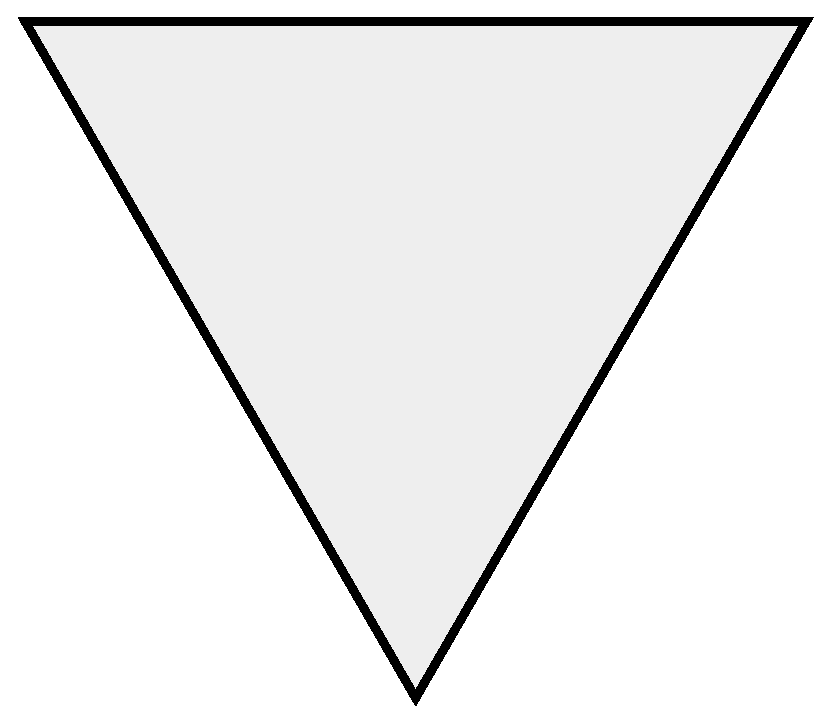
\includegraphics[scale=.15]{pics/Koch_Snowflake-0}
\end{minipage}
\hfill
\begin{minipage}{.24\textwidth}
\centering
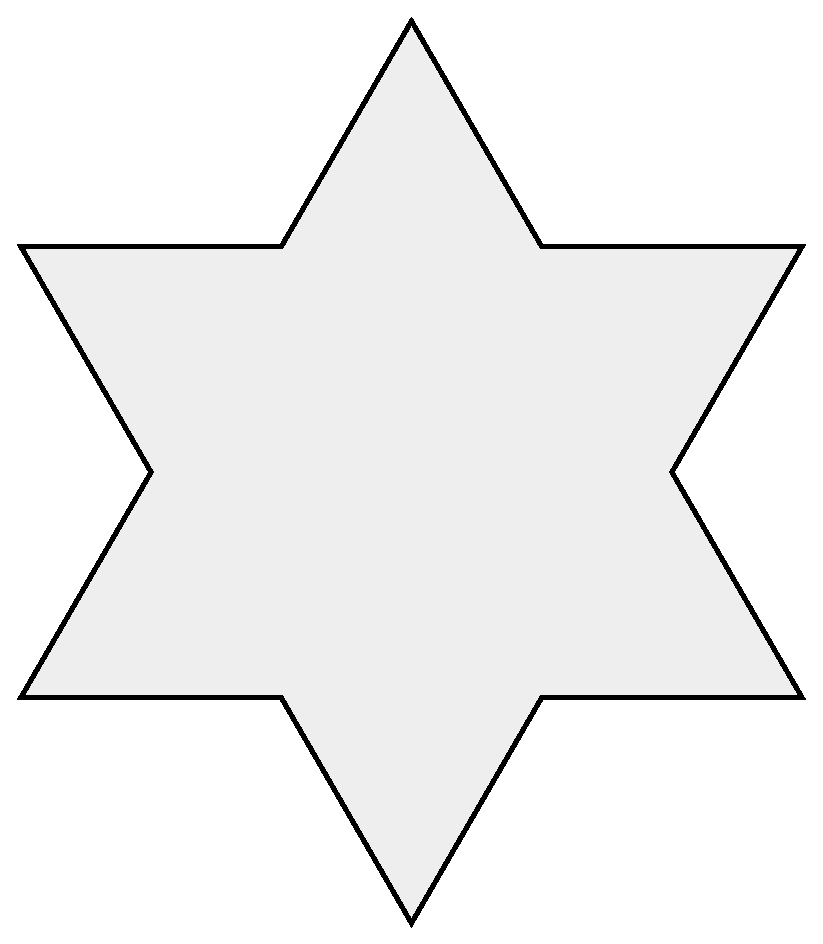
\includegraphics[scale=.15]{pics/Koch_Snowflake-1}
\end{minipage}
\hfill
\begin{minipage}{.24\textwidth}
\centering
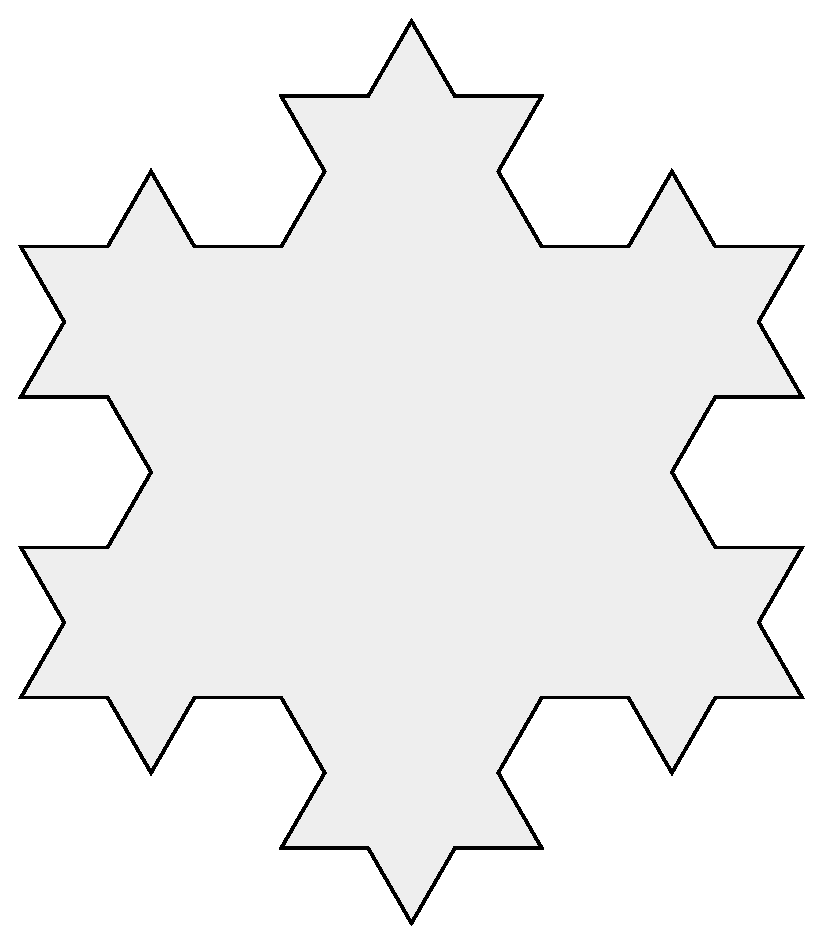
\includegraphics[scale=.15]{pics/Koch_Snowflake-2}
\end{minipage}
\hfill
\begin{minipage}{.24\textwidth}
\centering
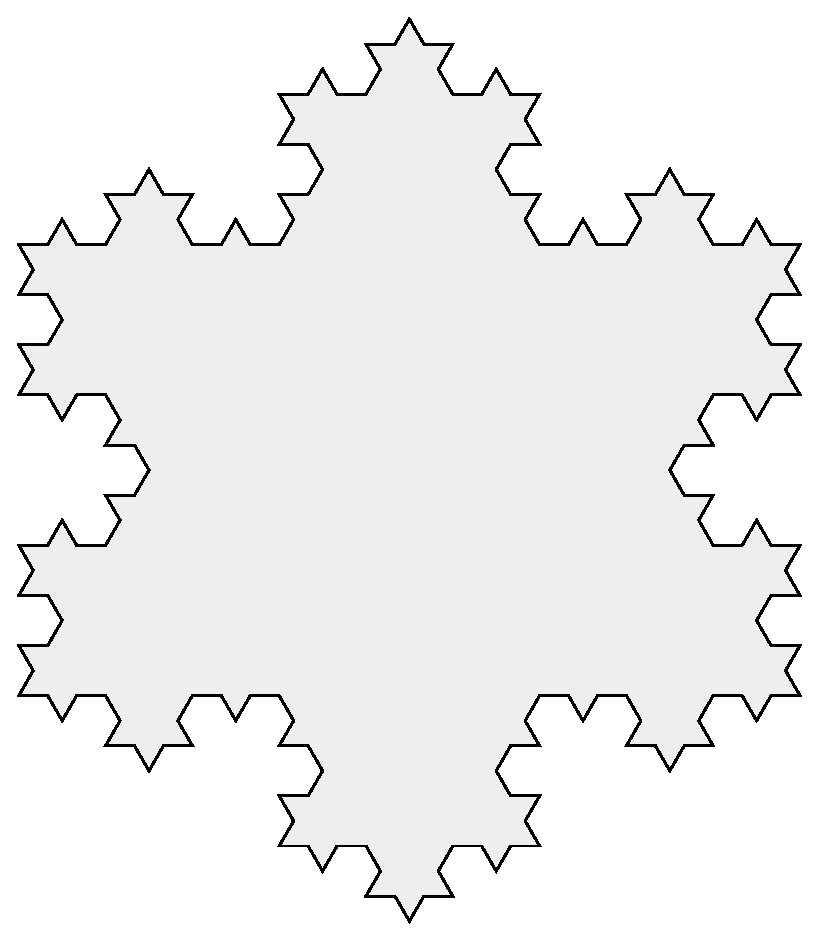
\includegraphics[scale=.15]{pics/Koch_Snowflake-3}
\end{minipage}
\end{figure}
Few first iterations of the construction are shown on the diagram.
The Koch snowflake is the boundary of the union of all the polygons.


\begin{thm}{Exercise}\label{ex:nonrectifiable-curve}
\begin{enumerate}[(a)]
\item Show that Koch snowflake is a closed simple curve; that is, it admits a homeomorphism to a circle.
\item\label{ex:nonrectifiable-curve:b} Show that Koch snowflake is not rectifiable. 
\end{enumerate}
\end{thm}


\section*{Arc length parametrization}

We say that a parametrized curve $\gamma$ has an \emph{arc length parametrization}\footnote{which is also called \emph{natural parametrization}}
if for any two values of parameters $t_1<t_2$, the value $t_2-t_1$ is the length of $\gamma|_{[t_1,t_2]}$; that is, the closed arc of $\gamma$ from $t_1$ to $t_2$.

Note that a smooth space curve $\gamma(t)=(x(t),y(t),z(t))$ has arc length parametrization if and only if it has unit velocity vector at all times;
that is 
\[|\gamma'(t)|=\sqrt{x'(t)^2+y'(t)^2+z'(t)^2}=1;\]
by that reason arc length parametrization of smooth curves with also called \emph{unit-speed curves}.
Note that smooth unit-speed curves are automatically regular.


Any rectifiable curve can be parameterized by arc length.
For a parametrized smooth curve $\gamma$, the arc length parameter $s$ can be written as an integral
\[s(t)=\int_{t_0}^t |\gamma'(\tau)|\cdot d\tau.\]
Note that $s(t)$ is a smooth increasing function.
Further by fundamental theorem of calculus, $s'(t)=|\gamma'(t)|$.
Therefore if $\gamma$ is regular, then $s'(t)\ne0$ for any parameter value $t$.
By inverse function theorem (\ref{thm:inverse}) the inverse function $s^{-1}(t)$ is also smooth.
Therefore $\gamma\circ s^{-1}$ --- the reparametrization  of $\gamma$ by arclength  $s$ --- remains smooth and regular.

Most of the time we use $s$ for an arc length parameter of a curve.

\begin{thm}{Exercise}\label{ex:arc-length-helix}
Reparametrize the helix 
\[\gamma_{a,b}(t)=(a\cdot\cos t,a\cdot \sin t, b\cdot t)\]
by arc length.
\end{thm}

We will be interested in the properties of curves that are invariant under a reparametrization.
Therefore we can always assume that the given smooth regular curve comes with a arc length parametrization.
A good property of arc length parametrizations is that it is almost canonical --- these parametrizations differ only by a sign and additive constant.
On the other hand, often it is impossible to find an arc length parametrization in a closed form which makes it hard to use it calculations;
usually it is more convenient to use the original parametrization.

\section*{Convex curves}

A simple plane curve is called \emph{convex} if it bounds a convex region.

\begin{thm}{Proposition}\label{prop:convex-curve}
Assume a convex closed curve $\alpha$ lies inside the domain bounded by a closed simple plane curve $\beta$.
Then
\[\length\alpha\le \length\beta.\]
\end{thm}

Note that it is sufficient to show that for any polygon  $P$ inscribed in $\alpha$ there is a polygon $Q$ inscribed in $\beta$ with 
$\perim P\le \perim Q$, where $\perim P$ denotes the perimeter of $P$.

Therefore it is sufficient to prove the following lemma.


\begin{thm}{Lemma}\label{lem:perimeter}
Let $P$ and $Q$ be polygons.
Assume $P$ is convex and $Q\supset P$.
Then 
\[\perim P\le \perim Q.\]

\end{thm}


\begin{wrapfigure}{r}{24 mm}
\vskip-4mm
\centering
\includegraphics{mppics/pic-7}
%\caption*{}
\end{wrapfigure}

\parit{Proof.}
Note that by the triangle inequality,
the inequality
\[\perim P\le \perim Q\]
holds
if $P$ can be obtained from $Q$ by cutting it along a chord;
that is, a line segment with ends on the boundary of $Q$ that lies in $Q$.


Note that there is an increasing sequence of polygons 
$$P=P_0\subset P_1\subset\dots\subset P_n=Q$$
such that $P_{i-1}$ obtained from $P_{i}$ by cutting along a chord.
Therefore 
\begin{align*}
\perim P=\perim P_0&\le\perim P_1\le\dots
\\
\dots&\le\perim P_n=\perim Q
\end{align*}
and the lemma follows.
\qeds

\begin{thm}{Corollary}
Any convex closed plane curve is rectifiable.  
\end{thm}

\parit{Proof.}
Any closed curve is bounded; that is, it lies in a sufficiently large square.
Indeed the curve can be described as an image of a loop $\alpha\:[0,1]\to\RR^2$, $\alpha(t)=(x(t),y(t))$.
The coordinate functions $x(t)$ and $y(t)$ are continous functions defined on $[0,1]$.
Therefore the absolute values of both of these functions are bounded by some constant $C$.
That is $\alpha$ lies in the square defined by the inequalities $|x|\le C$ and $|y|\le C$.

By Proposition~\ref{prop:convex-curve}, the length of the curve can not exceed the perimeter of the square $8\cdot C$, whence the result.
\qeds

Recall that convex hull of a set $X$ is the smallest convex set that contains $X$; in other words convex hull is the intersection of all convex sets containing $X$.

\begin{thm}{Exercise}\label{ex:convex-hull}
Let $\alpha$ be a closed simple plane curve.
Denote by $K$ the convex hull of $\alpha$; let $\beta$ be the boundary curve of $K$.
Show that 
\[\length \alpha\ge \length \beta.\]

Try to show that the statement holds for arbitrary closed plane curve $\alpha$, assuming that $X$ has nonempty interior.
\end{thm}


\section*{Crofton formulas*}

Consider a plane curve $\alpha\:[a,b]\to\RR^2$.
Given a unit vector $u$, denote by $\alpha_u$ the curve that follows orthogonal projections of $\alpha$ to the line in the direction $u$;
that is 
\[\alpha_u(t)=\langle u,\alpha(t)\rangle\cdot u.\]

Note that 
\[|\alpha'(t)|=|\langle u,\alpha'(t)\rangle|\] for any $t$.
Note that for any plane vector the magnitude of its average projection is proportional to its magnitude with coefficient; that is,
\[|w|=k\cdot \overline{|w_u|},\]
where $\overline{|w_u|}$ denotes the average value of $|w_u|$ for all unit vectors $u$.
(The value $k$ is the average value of $|\cos\phi|$ for $\phi\in [0,2\cdot\pi]$; it can be found by integration, but soon we will show another way to find it.)

If the curve $\alpha$ is smooth, then according to Exercise~\ref{ex:integral-length}
\begin{align*}
\length\alpha
&=\int_a^b|\alpha'(t)|\cdot dt=
\\
&=\int_a^b  k\cdot \overline{|\alpha_u'(t)|}\cdot dt=
\\
&=k\cdot \overline{\length\alpha_u}.
\end{align*}
This formula and its relatives are called Crofton formulas.
To find the coefficient $k$ one can apply it for the unit circle: the left hand side is $2\cdot\pi$ --- this is the length of unit circle.
Note that for any unit vector $u$, the curve $\alpha_u$ runs back and forth along an interval of length 2.
Therefore $\length\alpha_u=4$ and hence its average value is also 4.
It follows that the coefficient $k$ has to satisfy the equation $2\cdot \pi =k\cdot 4$; whence 
\[
\length\alpha
=\tfrac\pi2\cdot \overline{\length\alpha_u}.
\]

The Crofton's formula holds for arbitrary rectifiable curves, not necessary smooth; it can be proved using Exercises~\ref{adex:integral-length}.

\begin{thm}{Exercise}\label{ex:convex-croftons}
Show that any closed plane curve $\alpha$ has length at least $\pi\cdot s$, where $s$ is the average of pojections of $\alpha$ to lines.
Moreover the equality holds if and only if $\alpha$ is convex.

Use this statement to give another solution of Exercise~\ref{ex:convex-hull}.
\end{thm}

\begin{thm}{Advanced exercise}\label{adex:more-croftons}
Show that the length of space curve is proportional to the average length of its projections to all lines and to planes.
Find the coefficients in each case.
\end{thm}


\begin{thm}{Advanced exercises}\label{adex:integral-length}
\begin{enumerate}[(a)]
\item Show that the formula \ref{eq:length} holds for any Lipschitz curve $\alpha\:[a,b]\z\to\RR^3$.
\item Construct a simple curve $\alpha\:[a,b]\to\RR^3$ such that the velocity vector $\alpha'(t)$ is defined and bounded for almost all $t\in [a,b]$, but the formula \ref{eq:length} does not hold.

\end{enumerate}
\end{thm}

\parit{Hint:} Use theorems of Rademacher and Lusin (\ref{thm:rademacher} and \ref{thm:lusin}).

\section*{Semicontinuity of length}

Recall that the lower limit 
of a sequence of real numbers $(x_n)$ is denoted by
\[\liminf_{n\to\infty} x_n.\] 
It is defined as the lowest partial limit; that is, the lowest possible limit of a subsequence of $(x_n)$.
The lower limit is defined for any sequence of real numbers and it lies in the exteded real line $[-\infty,\infty]$


\begin{thm}{Theorem}\label{thm:length-semicont}
Length is a lower semi-continuous with respect to pointwise convergence of curves. 

More precisely, assume that a sequence
of curves $\alpha_n\:[a,b]\to \spc{X}$ in a metric space $\spc{X}$ converges pointwise 
to a curve $\alpha_\infty\:[a,b]\to \spc{X}$;
that is, $\alpha_n(t)\z\to\alpha_\infty(t)$ for any fixed $t\in[a,b]$ as $n\to\infty$. 
Then 
$$\liminf_{n\to\infty} \length\alpha_n \ge \length\alpha_\infty.\eqlbl{eq:semicont-length}$$
\end{thm}



\begin{wrapfigure}{r}{20 mm}
\vskip-0mm
\centering
\includegraphics{mppics/pic-6}
\end{wrapfigure}


Note that the inequality \ref{eq:semicont-length} might be strict.
For example the diagonal $\alpha_\infty$ of the unit square 
can be  approximated by a sequence of stairs-like
polygonal curves $\alpha_n$
with sides parallel to the sides of the square ($\alpha_6$ is on the picture).
In this case
\[\length\alpha_\infty=\sqrt{2}\quad
\text{and}\quad \length\alpha_n=2\]
for any $n$.

\parit{Proof.}
Fix a partition $a=t_0<t_1<\dots<t_k=b$.
Set 
\begin{align*}\Sigma_n
&\df
|\alpha_n(t_0)-\alpha_n(t_1)|+\dots+|\alpha_n(t_{k-1})-\alpha_n(t_k)|.
\\
\Sigma_\infty
&\df
|\alpha_\infty(t_0)-\alpha_\infty(t_1)|+\dots+|\alpha_\infty(t_{k-1})-\alpha_\infty(t_k)|.
\end{align*}

Note that $\Sigma_n\to \Sigma_\infty$ as $n\to\infty$
and $\Sigma_n\le\length\alpha_n$ for each $n$.
Hence
$$\liminf_{n\to\infty} \length\alpha_n \ge \Sigma_\infty.\eqlbl{>=Sigma-infty}$$

If $\alpha_\infty$ is rectifiable, we can assume that 
\begin{align*}
\length\alpha_\infty<\Sigma_\infty+\eps.
\end{align*}
for any given $\eps>0$.
By \ref{>=Sigma-infty} it follows that 
$$\liminf_{n\to\infty} \length\alpha_n > \length\alpha_\infty-\eps$$
for any $\eps>0$; whence \ref{eq:semicont-length} follows.

It remains to consider the case when $\alpha_\infty$ is not rectifiable; 
that is $\length\alpha_\infty=\infty$.
In this case we can choose a partition so that $\Sigma_\infty>L$ for any real number $L$.
By \ref{>=Sigma-infty} it follows that 
$$\liminf_{n\to\infty} \length\alpha_n > L$$
for any $L$; whence 
\[\liminf_{n\to\infty}\length\alpha_n=\infty\]
and \ref{eq:semicont-length} follows.
\qeds

\section*{Length metric}

Let $\spc{X}$ be a metric space.
Given two points $x,y$ in $\spc{X}$, denote by $d(x,y)$ the exact lower bound for lengths of all paths connecting $x$ to $y$; if there is no such path we assume that $d(x,y)=\infty$.

Note that function $d$ satisfies all the axioms of metric except it might take infinite value.
Therefore if any two points in $\spc{X}$ can be connected by a rectifiable curve, then $d$ defines a new metric on $\spc{X}$; in this case $d$ is called \emph{induced length metric}.

Evidently $d(x,y)\ge |x-y|$ for any pair of points $x,y\in \spc{X}$.
If the equality holds for any pair, then then the metric is called \emph{length metric} and the space is called \emph{length-metric space}.

Most of the time we consider length-metric spaces.
In particular the Euclidean space is a length-metric space.
A subspaces $A$ of length-metric space $\spc{X}$ might be not a lenght-metric space;
the induced length distance between points $x$ and $y$ in the subspace $A$ will be denoted as $|x-y|_A$;
that is $|x-y|_A$ is the exact lower bound for the length of paths in $A$.

\begin{thm}{Exercise}\label{ex:intrinsic-convex}
Let $A\subset \RR^3$ be a closed subset.
Show that $A$ is convex if and only if
\[|x-y|_A=|x-y|_{\RR^3}.\]
\end{thm}

\begin{thm}{Exercise}\label{ex:S1-intrinsic}
Let us denote by $\SS^1$ the unit circle in the plane; that is,
\[\SS^1=\set{(x,y)\in\RR^3}{x^2+y^2=1}.\]
Show that
\[|u-v|_{\SS^1}=\measuredangle(u,v)\df\arccos\langle u,v\rangle\]
for any $u,v\in \SS^1$.
\end{thm}

\section*{Spherical curves}

A space curve $\gamma$ is called \emph{spherical} if it runs in the unit sphere;
that is, $|\gamma(t)|=1$ for any $t$.

\begin{thm}{Exercise}\label{ex:S2-intrinsic}
Let us denote by $\SS^2$ the unit sphere in the space; that is,
\[\SS^2=\set{(x,y,z)\in\RR^3}{x^2+y^2+z^2=1}.\]
Show that
\[|u-v|_{\SS^2}=\measuredangle(u,v)\df\arccos\langle u,v\rangle\]
for any $u,v\in \SS^2$.
\end{thm} %???spherical geometry

\parit{Hint:} Use Exercise~\ref{ex:S1-intrinsic} and the following map $f\:(r,\theta,\phi)\mapsto (r,\theta,0)$ in spherical coordinates. Note that $f$ is distance nonexpanding and it maps $\RR^3$ to a half-plane and $\SS^2$ to one of its meridians.

\begin{thm}{Hemisphere lemma}\label{lem:hemisphere}
Any closed curve of length $<2\cdot \pi$ in $\SS^2$ lies in an open hemisphere. 
\end{thm}

This lemma is a keystone in the proof of Fenchel's theorem given below.
The lemma is not as simple as you might think --- try to prove it yourself.
I learned the following proof from Stephanie Alexander.

\parit{Proof.}
Let $\alpha$ be a closed curve in $\mathbb{S}^2$ of length $2\cdot\ell$.

%???+PIC

Assume $\ell<\pi$.

\begin{wrapfigure}{r}{35 mm}
\vskip-0mm
\centering
\includegraphics{mppics/pic-52}
\caption*{The north hemisphere corresponds to the disc and the south hemisphere to the complement of the disc.}
\end{wrapfigure}

Let us divide $\alpha$ into two arcs $\alpha_1$ and $\alpha_2$ of length $\ell$, with endpoints $p$ and $q$. 
According to Exercise~\ref{ex:S2-intrinsic}, $\measuredangle(p,q)\le\ell<\pi$.
Denote by $z$ be the midpoint between $p$ and $q$ in $\mathbb{S}^2$;
that is $z$ is the midpoint of an equator arc from $p$ to $q$. 
We claim that $\alpha$ lies in the open north hemisphere with north pole at $z$.  
If not, $\alpha$ intersects the equator in a point, say $r$.
Without loss of generality we may assume that $r$ lies on~$\alpha_1$. 

Rotate the arc $\alpha_1$ by angle $\pi$ around the line thru $z$ and the center of the sphere.
The obtained arc $\alpha_1^{*}$ together with $\alpha_1$ forms a closed curve of length $2\cdot \ell$ that passes thru $r$ and its antipodal point $r^{*}$.
Therefore
\[\tfrac12\cdot\length \alpha=\ell\ge \measuredangle(r,r^{*})=\pi,\] 
a contradiction.
\qeds

\begin{thm}{Exercise}\label{ex:antipodal}
Describe a simple closed spherical curve that does not pass thru a pair of antipodal points and does not lie in any hemisphere.
\end{thm}


\begin{thm}{Exercise}\label{ex:bisection-of-S2}
Suppose that a closed simple spherical curve $\alpha$ divides $\SS^2$ into two regions of equal area.
Show that 
\[\length\alpha\ge2\cdot\pi.\]
\end{thm}


\begin{thm}{Exercise}\label{ex:flaw}
Consider the following problem, find a flaw in the given solution.
Come up with a correct argument.
\end{thm}

 
\parbf{Problem.}
Suppose that a closed plane curve $\alpha$ has length at most 4.
Show that $\alpha$ lies in a unit disc.

\parit{Wrong solution.}
Note that it is sufficient to show that diameter of $\alpha$ is at most 2;
that is, the distance between any two pairs of points $p$ and $q$ of $\alpha$ an not exceed $2$.

The length of $\alpha$ can not be smaller then the closed inscribed polygonal line which goes from $p$ to $q$ and back to $p$.
Therefore 
\[2\cdot |p-q|\le\length \alpha\le 4.\]
\qedsf

\begin{thm}{Advanced exercises} \label{adex:crofton}
Given points $v,w\in\SS^2$, denote by $w_v$ the closest point to $w_u$ on the equator with pole at $v$;
in other words, it $w^\perp$ is the projection of $w$ to the plane perpendicular to $v$, then $w_v$ is the unit vector in the direction of $w^\perp$.
The vector $w_v$ is defined if $w\ne\pm v$.

\begin{enumerate}
\item \label{adex:crofton:crofton}
Show that for any spherical curve $\alpha$ we have that
\[\length\alpha=\overline{\length\alpha_v},\]
where $\overline{\length\alpha_v}$ denotes the average length for all $v\in \SS^2$.
(This is a spherical analog of Crofton's formula.)
\item\label{adex:crofton:hemisphere} Give another proof of hemisphere lemme using part (\ref{adex:crofton:crofton}). 
\end{enumerate}
 
\end{thm}


\chapter{Curvature}

\section*{Acceleration of a unit-speed curve}

Recall that any regular smooth curve can be parameterized by its arc-length.
The obtained parameterized curve, say $\gamma$, remains to be smooth and it has unit speed; 
that is, $|\gamma'(s)|=1$ for all $s$.
The following proposition states that in this case
the acceleration vector stays perpendicular to the velocity vector.

\begin{thm}{Proposition}\label{prop:a'-pertp-a''}
Assume $\gamma$ is a smooth unit-speed space curve.
Then $\gamma'(s)\perp \gamma''(s)$ for any $s$.
\end{thm}

The scalar product (also known as dot product) of two vectors $\vec v$ and $\vec w$ will be denoted by $\langle \vec v,\vec w\rangle$.
Recall that the derivative of a scalar product satisfies the product rule;
that is, if $\vec v=\vec v(t)$ and $\vec w=\vec w(t)$ are smooth vector-valued functions of a real parameter $t$, then
\[\langle \vec v,\vec w\rangle'=\langle \vec v',\vec w\rangle+\langle \vec v,\vec w'\rangle.\]

\parit{Proof.}
The identity $|\gamma'|=1$ can be rewritten as $\langle\gamma',\gamma'\rangle=1$.
Differentiating both sides, 
\[2\cdot\langle\gamma'',\gamma'\rangle=\langle\gamma',\gamma'\rangle'=0,\]
whence $\gamma''\perp\gamma'$.
\qeds

\section*{Curvature}

For a unit-speed smooth space curve $\gamma$ the magnitude of its acceleration $|\gamma''(s)|$ is called its \emph{curvature} at the time $s$.
\label{page:curvature}
If $\gamma$ is simple, then we can say that $|\gamma''(s)|$ is the curvature at the point $p=\gamma(s)$ without ambiguity.
The curvature is usually denoted by $\kur(s)$ or $\kur(s)_\gamma$ and in the case of simple curves it might be also denoted by $\kur(p)$ or $\kur(p)_\gamma$.

The curvature measures how fast the curve turns;
if you drive along a plane curve, then curvature describes the position of your steering wheel at the given point (note that it does not depend on your speed).

In general, the term \emph{curvature} is used for anything that measures how much a \emph{geometric object} deviates from being \emph{straight};
for curves, it measures how fast it deviates from a straight line.

\begin{thm}{Exercise}\label{ex:curvature-of-spherical-curve}
Show that any regular smooth unit-speed spherical curve has curvature at least 1 at each time.
\end{thm}

\section*{Tangent indicatrix}

Let $\gamma$ be a regular smooth space curve.
Let us consider another curve 
\[\tan(t)=\tfrac{\gamma'(t)}{|\gamma'(t)|}\eqlbl{eq:tantrix}\] 
called \emph{tangent indicatrix} of $\gamma$.
Note that $|\tan(t)|=1$ for any $t$;
that is, $\tan$ is a spherical curve.


If $s\mapsto \gamma(s)$ is a unit-speed parametrization, then $\tan(s)=\gamma'(s)$.
In this case we have the following expression for curvature: 
\[\kur(s)\z=|\tan'(s)|\z=|\gamma''(s)|.\]

When $\gamma$ is not necessarily parameterized by arc-length, then
\[ \kur(t)=\frac{|\tan'(t)|}{|\gamma'(t)|}.\eqlbl{eq:curvature}\]
Indeed, for an arc-length parametrization $s(t)$ we have $s'(t)=|\gamma'(t)|$.
Therefore
\begin{align*}
\kur(t)&=\left|\frac{d\tan}{ ds}\right|=
\\
&=|\tfrac{d\tan}{ dt}|/|\tfrac{ds}{ dt}|=
\\
&=\frac{|\tan'(t)|}{|\gamma'(t)|}.
\end{align*}
It follows that the indicatrix of a smooth regular curve $\gamma$ is regular if the curvature of $\gamma$ does not vanish.

\begin{thm}{Exercise}\label{ex:curvature-formulas}
Use the formulas \ref{eq:tantrix} and \ref{eq:curvature} to show that 
for any smooth regular space curve $\gamma$ we have the following expressions for its curvature:

\begin{subthm}{ex:curvature-formulas:a} \[\kur(t)=\frac{|\vec w(t)|}{|\gamma'(t)|^2},\]
where $\vec w(t)$ denotes the projection of $\gamma''(t)$ to the plane normal to $\gamma'(t)$;
\end{subthm}

\begin{subthm}{ex:curvature-formulas:b}
\[\kur(t)=\frac{|\gamma''(t)\times \gamma'(t)|}{|\gamma'(t)|^{3}},\]
where $\times$ denotes the \emph{vector product} (also known as \emph{cross product}).
\end{subthm}

\end{thm}


\begin{thm}{Exercise}\label{ex:curvature-graph}
Apply the formulas in the previous exercise to show that if $f$ is a smooth real function,
then its graph $y=f(x)$  has curvature
\[\kur(p)=\frac{|f''(x)|}{(1+f'(x)^2)^{\frac32}}\]
at the point $p=(x,f(x))$.
\end{thm}

\section*{Tangent curves}

Let $\gamma$ be a smooth regular space curve and $\tan$ its tangent indicatrix.
The line thru $\gamma(t)$ in the direction of $\tan(t)$ is called the \emph{tangent line} at~$t$.

The tangent line could be also defined as a unique line that has that has \emph{first order of contact} with $\gamma$ at $s$;

that is, $\rho(\ell)=o(\ell)$, where $\rho(\ell)$ denotes the distance from $\gamma(s+\ell)$ to the line.

We say that smooth regular curve $\gamma_1$ at $s_1$ is \emph{tangent} to a smooth regular curve $\gamma_2$ at $s_2$
if $\gamma_1(s_1)=\gamma_2(s_2)$ and the tangent line of $\gamma_1$ at $s_1$ coincides with the tangent line of $\gamma_2$ at $s_2$;
if both curves are simple we can also say that they are tangent at the point $p=\gamma_1(s_1)\z=\gamma_2(s_2)$ without ambiguity.


\section*{Total curvature}

Let $\gamma\:\mathbb{I}\to\RR^3$ be a smooth unit-speed curve and $\tan$ its tangent indicatrix.
The integral 
\[\tc\gamma:=\int_{\mathbb{I}}\kur(s)\cdot ds\]
is called \emph{total curvature of}\label{page:total curvature of:smooth-def}
$\gamma$.

When $\gamma$ is not parameterized by arc-length, by a change of variables, the above integral takes the form

\[\tc\gamma:=\int_{\mathbb{I}}\kur( \gamma (t) ) | \gamma ' (t) | \cdot ds   \eqlbl{eq:tocurv} \]


\begin{thm}{Exercise}\label{ex:helix-curvature}
Find the curvature of the helix \[\gamma_{a,b}(t)=(a\cdot \cos t,a\cdot \sin t,b\cdot t),\] its tangent indicatrix and the total curvature of its  arc for $t\in[0,2\cdot\pi]$.
\end{thm}

\begin{thm}{Observation}\label{obs:tantrix}
The total curvature of a smooth regular curve is the length of its tangent indicatrix.
\end{thm}

\parit{Proof.}
Combine \ref{eq:tocurv} and \ref{eq:curvature}.
\qedsf %???other cases --- colsed curves, semiopen intervals...


\begin{thm}{Fenchel's theorem}\label{thm:fenchel}
The total curvature of any closed regular space curve is at least $2\cdot\pi$.
\end{thm}

\parit{Proof.}
Fix a closed regular space curve $\gamma$;
we can assume that it is described by a unit-speed loop $\gamma\:[a,b]\to \RR^3$;
in this case $\gamma(a)=\gamma(b)$ and $\gamma'(a)=\gamma'(b)$.

Consider its tangent indicatrix $\tan=\gamma'$.
Recall that $|\tan(s)|=1$ for any $s$; that is, $\tan$ is a closed spherical curve.

Let us show that $\tan$ cannot lie in a hemisphere.
Assume the contrary; without loss of generality we can assume that $\tan$ lies in the north hemisphere defined by the inequality $z>0$ in $(x,y,z)$-coordinates.
It means that $z'(t)>0$ for all $t$, where $\gamma(t)=(x(t), y(t), z(t))$.
Therefore 
\[z(b)-z(a)=\int_a^bz'(s)\cdot ds>0.\]
In particular, $\gamma(a)\ne \gamma(b)$, a contradiction.

Applying the observation (\ref{obs:tantrix}) and the hemisphere lemma (\ref{lem:hemisphere}), we get  
\[\tc\gamma=\length \tan\ge2\cdot\pi.\]
\qedsf

\begin{thm}{Exercise}\label{ex:length>=2pi}
Show that a closed space curve $\gamma$ with curvature at most~$1$ cannot be shorter than the unit circle;
that is, 
\[\length\gamma\ge 2\cdot \pi.\]

\end{thm}


\begin{thm}{Advanced exercise}\label{ex:gamma/|gamma|}
Suppose that $\gamma$ is a smooth regular space curve that does not pass thru the origin.
Consider the spherical curve defined as $\sigma(t)=\frac{\gamma(t)}{|\gamma(t)|}$ for any $t$.
Show that 
\[\length \sigma< \tc\gamma+\pi.\]
Moreover, if $\gamma$ is closed, then
\[\length \sigma\le \tc\gamma.\]
\end{thm}

Note that the last inequality gives an alternative proof of Fenchel's theorem.
Indeed, without loss of generality we can assume that the origin lies on a chord of $\gamma$.
In this case the closed spherical curve $\sigma$ goes from a point to its antipode and comes back; 
it takes length $\pi$ each way, 
whence 
\[\length\sigma\ge 2\cdot\pi.\]



\section*{Piecewise smooth curves}



Assume $\alpha\:[a,b]\to \RR^3$ and $\beta\:[b,c]\z\to \RR^3$ are two curves such that $\alpha(b)=\beta(b)$.
Then one can combine these two curves into one $\gamma\:[a,c]\z\to \RR^3$ by the rule 
\[\gamma(t)=
\begin{cases}
\alpha(t)&\text{if}\quad t\le b,
\\
\beta(t)&\text{if}\quad t\ge b.
\end{cases}
\]
The obtained curve $\gamma$ is called the 
\emph{concatenation} of $\alpha$ and $\beta$. %briefly $\gamma=\alpha{*}\beta$.
(The condition $\alpha(b)=\beta(b)$ ensures that the map $t\mapsto\gamma(t)$ is continuous.)

The same definition of concatenation can be applied if $\alpha$ and/or $\beta$ are defied on semiopen intervals 
$(a,b]$ and/or $[b,c)$.

\begin{wrapfigure}{o}{25 mm}
\vskip-2mm
\centering
\includegraphics{mppics/pic-54}
\end{wrapfigure}

The concatenation can be also defined if the end point of the first curve coincides with the starting point of the second curve;
if this is the case, then the time intervals of both curves can be shifted so that they fit together. 

If in addition $\beta(c)=\alpha(a)$, then we can do cyclic concatination of these curves;
this way we obtain a closed curve.

If $\alpha'(b)$ and $\beta'(b)$ are defined, then the angle $\theta=\measuredangle(\alpha'(b),\beta'(b))$ is called \emph{external angle} of $\gamma$ at time $b$.
If $\theta=\pi$, then we say that $\gamma$ has a \emph{cusp} at  time $b$.

Clearly, the assumption that the intervals $[a,b]$ and $[b,c]$ fit together is not essential, and we can concatenate any two curves $\alpha$ and $\beta$ as long as the endpoint of $\alpha$ coincides with the starting point of~$\beta$. 

A space curve $\gamma$ is called \emph{piecewise smooth and regular} if it can be presented as an iterated concatination of a finite number of smooth regular curves; if $\gamma$ is closed, then the  concatination is assumed to be cyclic.

If $\gamma$ is a concatination of smooth regular arcs $\gamma_1,\dots,\gamma_n$, then the total curvature of $\gamma$ is defined as a sum of the total curvatures of $\gamma_i$ and the external angles;
that is, 
\[\tc\gamma=\tc{\gamma_1}+\dots+\tc{\gamma_n}+\theta_1+\dots+\theta_{n-1}\]
where $\theta_i$ is the external angle at the joint between $\gamma_i$ and $\gamma_{i+1}$;
if $\gamma$ is closed, then 
\[\tc\gamma=\tc{\gamma_1}+\dots+\tc{\gamma_n}+\theta_1+\dots+\theta_{n},\]
where $\theta_n$ is the external angle at the joint between $\gamma_n$ and $\gamma_1$.

In particular, for a smooth regular loop $\gamma:[a,b] \to \mathbb{R}^3$, the total curvature of the corresponding closed curve $\hat\gamma$ is defined as
\[\tc{\hat\gamma}\df\tc\gamma + \theta,\]
where $\theta=\measuredangle(\gamma'(a),\gamma'(b))$.

\begin{thm}{Generalized Fenchel's theorem}\label{thm:gen-fenchel}
Let $\gamma$ be a closed piecewise smooth regular space curve.
Then 
\[\tc\gamma\ge2\cdot\pi.\]

\end{thm}

\parit{Proof.}
Suppose $\gamma$ is a cyclic concatenation of $n$ smooth regular arcs $\gamma_1,\dots,\gamma_n$.
Denote by $\theta_1,\dots,\theta_n$ its external angles.
We need to show that
\[\tc{\gamma_1}+\dots+\tc{\gamma_n}+\theta_1+\dots+\theta_n\ge2\cdot\pi.\eqlbl{eq:gen-fenchel}\]

Consider the tangent indicatrix $\tan_1,\dots,\tan_n$ for each arc $\gamma_1,\dots,\gamma_n$;
these are smooth spherical arcs.

The same argument as in the proof of Fenchel's theorem, shows that the curves $\tan_1,\dots,\tan_n$ cannot lie in an open hemisphere.

Note that the spherical distance from the end point of $\tan_i$ to the starting point of $\tan_{i+1}$ is equal to the external angle $\theta_i$ (we enumerate the arcs modulo $n$, so $\gamma_{n+1}=\gamma_1$).
Let us connect the end point of $\tan_i$ to the starting point of $\tan_{i+1}$ by a short arc of a great circle in the sphere.
This way we get a closed spherical curve that is $\theta_1+\dots+\theta_n$ longer then the total length of $\tan_1,\dots,\tan_n$.

Applying the hemisphee lemma (\ref{lem:hemisphere}) to the obtained closed curve, we get that
\[\length\tan_1+\dots+\length\tan_n+\theta_1+\dots+\theta_n\ge 2\cdot\pi.\]
Applying the observation (\ref{obs:tantrix}), we get \ref{eq:gen-fenchel}.
\qedsf

\begin{thm}{Chord lemma}\label{lem:chord}
Let $\ell$ be the chord to a smooth regular arc $\gamma\:[a,b]\to\RR^3$.
Assume $\gamma$ meets $\ell$ at angles $\alpha$ and $\beta$ at $\gamma (a)$ and $\gamma (b)$, respectively;
that is 
\[\alpha=\measuredangle(\vec w,\gamma'(a))\quad\text{and}\quad \beta=\measuredangle(\vec w,\gamma'(b)),\]
where $\vec w=\gamma(b)-\gamma(a)$.
Then 
\[\tc\gamma\ge \alpha+\beta.\eqlbl{tc>a+b}\] 

\end{thm}

\begin{wrapfigure}{o}{45 mm}
\vskip-0mm
\centering
\includegraphics{mppics/pic-53}
\vskip0mm
\end{wrapfigure}

%??? is it really due to Reshetnyak???

\parit{Proof.}
Let us parameterize the chord $\ell$ from $\gamma(b)$ to $\gamma(a)$ and consider the cyclic concatenation $\bar\gamma$ of $\gamma$ and $\ell$.
The closed curve $\bar\gamma$ has two external angles $\pi-\alpha$ and $\pi-\beta$.
Since the curvature of $\ell$ vanishes, we get 
\[\tc{\bar\gamma}=\tc\gamma+(\pi-\alpha)+(\pi-\beta).\]
According to the generalized Fenechel's theorem (\ref{thm:gen-fenchel}),
$\tc{\bar\gamma}\ge 2\cdot\pi$;
hence \ref{tc>a+b} follows.
\qeds

\begin{thm}{Exercise}\label{ex:chord-lemma-optimal}
Show that the estimate in the chord lemma is optimal.
That is, given two points $p, q$ and two unit vectors $u,v$ in $\RR^3$,
show that there is a smooth regular curve $\gamma$ that starts at $p$ in the direction $\vec u$ and ends at $q$ in the direction $\vec v$ such that 
$\tc\gamma$ is arbitrarily close to $\measuredangle(\vec w,\vec u)+\measuredangle(\vec w,\vec v)$, where $\vec w=q-p$.

\end{thm}

\section*{Polygonal lines} 

Polygonal lines are a particular case of piecewise smooth regular curves;
each arc in its concatenation is a line segment.
Since the curvature of a line segment vanishes, the total curvature of a polygonal line is the sum of its external angles.

\begin{thm}{Exercise}\label{ex:monotonic-tc}
Let $a,b,c,d$ and $x$ be distinct points in $\RR^3$.
Show that the total curvature of the polygonal line $abcd$ cannot exceed the total curvature of $abxcd$; that is, 
\[\tc {abcd} \leq \tc {abxcd}.\]

Use this statement to show that any closed polygonal line has curvature at least $2\cdot\pi$.
\end{thm}



\begin{thm}{Proposition}\label{prop:inscribed-total-curvature}
Assume a polygonal line $\beta=p_0\dots p_n$ is inscribed in a smooth regular curve $\gamma$.
Then 
\[\tc\gamma\ge \tc{\beta}.\]
Moreover if $\gamma$ is closed we allow the inscribed polygonal line $\beta$ to be closed.

\end{thm}

\parit{Proof.}
Since the curvature of line segments vanishes, 
the total curvature of polygonal line is the sum of external angles $\theta_i=\pi-\measuredangle p_{i-1}p_ip_{i+1}$.

\begin{wrapfigure}{o}{40 mm}
\vskip-0mm
\centering
\includegraphics{mppics/pic-55}
\vskip0mm
\end{wrapfigure}

Assume $p_i=\gamma(t_i)$.
Set 
\begin{align*}
\vec w_i&=p_{i+1}-p_i,& \vec v_i&=\gamma'(t_i),
\\
\alpha_i&=\measuredangle (\vec w_i,\vec v_i),&\beta_i&=\measuredangle (\vec w_{i-1},\vec v_i).
\end{align*}
In the case of a closed curve we use indexes modulo $n$, in particular $p_{n+1}\z=p_1$.

Note that $\theta_i=\measuredangle (\vec w_{i-1},\vec w_i)$.
By triangle inequality for angles \ref{thm:spherical-triangle-inq}, we get that
\[\theta_i\le \alpha_i+\beta_i.\]
By the chord lemma, the total curvature of the arc of $\gamma$ from $p_i$ to $p_{i+1}$ is at least $\alpha_i+\beta_{i+1}$. 

Therefore if $\gamma$ is a closed curve, we have
\begin{align*}
\tc{\beta}&=\theta_1+\dots+\theta_n\le 
\\
&\le\beta_1+\alpha_1+\dots+\beta_n+\alpha_n = 
\\
&=(\alpha_1+\beta_2)+\dots+(\alpha_n+\beta_1) \le 
\\
&\le \tc\gamma.
\end{align*}
If $\gamma$ is an arc, the argument is analogous:
\begin{align*}
\tc{\beta}&=\theta_1+\dots+\theta_{n-1}\le 
\\
&\le\beta_1+\alpha_1+\dots+\beta_{n-1}+\alpha_{n-1} \le
\\
&\le (\alpha_0+\beta_1)+\dots+(\alpha_{n-1}+\beta_n) \le 
\\
&\le \tc\gamma.
\end{align*}
\qedsf

\begin{thm}{Exercise}\label{ex:sef-intersection}

\begin{subthm}{ex:sef-intersection:<2pi}Draw a smooth regular plane curve $\gamma$ which has a self-intersection, such that $\tc\gamma<2\cdot\pi$.
\end{subthm}

\begin{subthm}{ex:sef-intersection:>pi} Show that if a smooth regular curve $\gamma\:[a,b]\to\RR^3$ has a self-intersection, then $\tc\gamma>\pi$.
\end{subthm}

\end{thm}

\begin{thm}{Proposition}\label{prop:fenchel=}
The equality case in the Fenchel's theorem holds only for convex plane curves;
that is, if the total curvature of a smooth regular space curve $\gamma$ equals $2\cdot\pi$, then $\gamma$ is a convex plane curve.
\end{thm}

The proof is an application of Proposition~\ref{prop:inscribed-total-curvature}.

\parit{Proof.}
Consider an inscribed quadraliteral $abcd$ in $\gamma$.
By the definition of total curvature, we have that
\begin{align*}
\tc{abcd}&=(\pi-\measuredangle dab)+(\pi-\measuredangle abc)+(\pi-\measuredangle bcd)+(\pi-\measuredangle cda)=
\\
&=4\cdot\pi -(\measuredangle dab+\measuredangle abc+\measuredangle bcd+\measuredangle cda))
\end{align*}


Note that 
\[
\measuredangle abc\le\measuredangle abd+ \measuredangle dbc
\quad\text{and}\quad
\measuredangle cda\le\measuredangle cdb+ \measuredangle bda.
\eqlbl{eq:spheric-triangle}
\]

The sum of angles in any triangle is $\pi$, so combining these inequalities, we get that 
\begin{align*}
\tc{abcd}&\ge 4\cdot \pi 
- (\measuredangle dab+\measuredangle abd+ \measuredangle bda)
-(\measuredangle bcd+\measuredangle cdb +\measuredangle dbc)=
\\
&=2\cdot\pi.
\end{align*}

\begin{wrapfigure}{r}{40 mm}
\vskip-7mm
\centering
\includegraphics{mppics/pic-56}
\vskip0mm
\end{wrapfigure}

By \ref{prop:inscribed-total-curvature},
\[\tc{abcd}\le \tc\gamma\le 2\cdot\pi.\]
Therefore we have equalities in \ref{eq:spheric-triangle}.
It means that the point $d$ lies in the angle $abc$ 
and the point $b$ lies in the angle $cda$.
That is, $abcd$ is a convex plane quadrilateral.

It follows that any quadrilateral inscribed in $\gamma$ is a convex plane quadrilateral.
Therefore all points of $\gamma$ lie in a fixed plane and the domain bounded by $\gamma$ in that plane is convex;
that is, $\gamma$ is a convex plane curve. %???more
\qeds

\begin{wrapfigure}{o}{30 mm}
\vskip-4mm
\centering
\includegraphics{mppics/pic-20}
\vskip0mm
\end{wrapfigure}

\begin{thm}{Exercise}\label{ex:quadrisecant}
Suppose that a closed curve $\gamma$ crosses a line at four points $a$, $b$, $c$ and $d$.
Assume that these points appear on the line in the order $a$, $b$, $c$, $d$
and they appear on the curve $\gamma$ in the order $a$, $c$, $b$, $d$.
Show that 
\[\tc\gamma\ge 4\cdot\pi.\]

\end{thm}

Lines crossing a curve at four points as in the above exercise are called \emph{alternating quadrisecants}.
It turns out that any \emph{nontrivial knot} admits an alternating quadrisecant \cite{denne};
according to the exercise the latter implies the so-called \emph{F\'ary--Milnor theorem} --- the total curvature any knot exceeds $4\cdot \pi$.

\section*{Bow lemma}

\begin{thm}{Lemma}\label{lem:bow}
Let $\gamma_1\:[a,b]\to\RR^2$ and $\gamma_2\:[a,b] \to\RR^3$ be two smooth unit-speed curves.
Suppose that $\kur(s)_{\gamma_1}\ge\kur(s)_{\gamma_2}$ for any $s$ 
and the curve
$\gamma_1$ is a simple arc of a convex curve; that is, it runs in the boundary of a covex plane figure.
Then the distance between the ends of $\gamma_1$ cannot exceed the  distance between the ends of $\gamma_2$; that is,
\[|\gamma_1(b)-\gamma_1(a)|\le |\gamma_2(b)-\gamma_2(a)|.\]

\end{thm}

The following exercise states that the condition that $\gamma_1$ is a convex arc is necessary.
It is instructive to do this exercise before reading the proof of the lemma.

\begin{thm}{Exercise}\label{ex:anti-bow}
Construct a simple smooth unit-speed plane curves $\gamma_1,\gamma_2\:[a,b]\to\RR^2$ such that 
that $\kur(s)_{\gamma_1}>\kur(s)_{\gamma_2}$ for any $s$ and
\[|\gamma_1(b)-\gamma_1(a)|> |\gamma_2(b)-\gamma_2(a)|.\]
\end{thm}


\begin{wrapfigure}{o}{36 mm}
\vskip-7mm
\centering
\includegraphics{mppics/pic-57}
\vskip0mm
\end{wrapfigure}

\parit{Proof.}
Denote by $\tan_1$ and $\tan_2$ the tangent indicatrixes of $\gamma_1$ and $\gamma_2$, respectively.

Let $\gamma_1(s_0)$ be the point on $\gamma_1$ furthest to the line 
thru $\gamma(a)$ and $\gamma(b)$.
Consider two unit vectors 
\[\vec u_1=\tan_1(s_0)=\gamma_1'(s_0)
\quad\text{and}\quad
\vec u_2=\tan_2(s_0)=\gamma_2'(s_0).\]
By construction, the vector $\vec u_1$ is parallel to $\gamma(b)-\gamma(a)$, in particular
\[|\gamma_1(b)-\gamma_1(a)|=\langle \vec u_1,\gamma_1(b)-\gamma_1(a)\rangle \]

Since $\gamma_1$ is an arc of a convex curve, its indicatrix $\tan_1$ runs in one direction along the unit circle.
Suppose $s\le s_0$, then 
\begin{align*}
\measuredangle(\gamma'_1(s),\vec u_1)&=\measuredangle(\tan_1(s),\tan_1(s_0))=
\\
&=\length (\tan_1|_{[s,s_0]})=
\\
&=\int_s^{s_0}|\tan_1'(t)|\cdot d t=
\\
&=\int_s^{s_0}\kur_1(t)\cdot d t\ge
\\
&\ge
\int_s^{s_0}\kur_2(t)\cdot d t=
\\
&=\int_s^{s_0}|\tan_2'(t)|\cdot d t= 
\\
&=\length (\tan_1|_{[s,s_0]})\ge
\\
&\ge \measuredangle(\tan_2(s),\tan_2(s_0))=
\\
&= \measuredangle(\gamma'_2(s),\vec u_2).
\end{align*}
That is, 
\[\measuredangle(\gamma'_1(s),\vec u_1)\ge \measuredangle(\gamma'_2(s),\vec u_2)\]
if $s\ge s_0$.
The same argument shows that 
\[\measuredangle(\gamma'_1(s),\vec u_1)\ge \measuredangle(\gamma'_2(s),\vec u_2)\eqlbl{<gamma',u>}\]
for $s\ge s_0$; therefore the inequality holds for any $s$.

Since $\vec u_1$ is a unit vector parallel to $\gamma_1(b)-\gamma_1(a)$, we have that
\[|\gamma_1(b)-\gamma_1(a)|=\langle \vec u_1,\gamma_1(b)-\gamma_1(a)\rangle\]
and since $\vec u_2$ is a unit vector, we have that
\[|\gamma_2(b)-\gamma_2(a)|\ge\langle \vec u_2,\gamma_2(b)-\gamma_2(a)\rangle\]

Integrating \ref{<gamma',u>}, we get 
\begin{align*}
|\gamma_1(b)-\gamma_1(a)|&=\langle \vec u_1,\gamma_1(b)-\gamma_1(a)\rangle=
\\
&=\int_a^b\langle \vec u_1,\gamma'_1(s)\rangle\cdot ds \le 
\\
&\le\int_a^b\langle \vec u_2,\gamma'_2(s)\rangle\cdot ds =
\\
&=\langle \vec u_2,\gamma_2(b)-\gamma_2(a)\rangle \le
\\
&\le |\gamma_2(b)-\gamma_2(a)|.
\end{align*}
Hence the result.\qeds

\begin{thm}{Exercise}\label{ex:length-dist}
Let $\gamma\:[a,b]\to \RR^3$ be a smooth regular curve and $0<\theta\le\tfrac\pi2$.
Assume 
\[\tc\gamma\le 2\cdot\theta.\]

\begin{subthm}{ex:length-dist:>} Show that
\[|\gamma(b)-\gamma(a)|> \cos\theta\cdot\length\gamma.\]
\end{subthm}

\begin{subthm}{} Use part \ref{SHORT.ex:length-dist:>} to give another solution of \ref{ex:sef-intersection:>pi}.
\end{subthm}

\begin{subthm}{} Show that the inequality in \ref{SHORT.ex:length-dist:>} is optimal; that is, given 
$\theta$ there is a smooth regular curve $\gamma$ such that $\frac{|\gamma(b)-\gamma(a)|}{\length\gamma}$ is arbitrarily close to $\cos\theta$.
\end{subthm}

\end{thm}



\begin{thm}{Exercise}\label{ex:schwartz}
Let $p$ and $q$ be points in a unit circle dividing it in two arcs with lengths $\ell_1<\ell_2$.
Suppose the space curve $\gamma$ connects $p$ to $q$ and has curvature at most 1. Show that either
\[\length \gamma\le \ell_1
\quad\text{or}\quad
\length \gamma\ge \ell_2.
\]
\end{thm} %H. A. Schwartz???

The following exercise generalizes \ref{ex:length>=2pi}.

\begin{thm}{Exercise}\label{ex:loop}
Suppose $\gamma\:[a,b]\to \RR^3$ is a smooth regular loop with curvature at most 1.
Show that 
\[\length\gamma\ge2\cdot\pi.\]

\end{thm}


\section*{DNA inequality*}

Recall that the curvature of a spherical curve is at least $1$
(Exercise~\ref{ex:curvature-of-spherical-curve}).
In particular, the length of a spherical curve cannot exceed its total curvature.
The following theorem shows that the same inequality holds for \emph{closed} curves in a unit ball.

\begin{thm}{Theorem}\label{thm:DNA}
Let $\gamma$ be a smooth regular closed curve that lies in a unit ball.
Then 
\[\tc\gamma\ge \length\gamma.\]

\end{thm}

This theorem was proved by Don Chakerian \cite{chakerian};
for plane curves it was proved earlier by Istv\'{a}n F\'{a}ry \cite{fary-DNA}.
We present the proof given by Don Chakerian in \cite{chakerian-short};
few other proofs of this theorem are discussed by Serge Tabachnikov~\cite{tabachnikov}.

\parit{Proof.}
Without loss of generality we can assume the curve is described by a loop $\gamma\:[0,\ell]\to\RR^3$ parameterized by its arc-length, so $\ell=\length\gamma$.
We can also assume that the origin is the center of the ball.
It follows that
\[\langle\gamma'(s),\gamma'(s)\rangle=1,\qquad |\gamma(s)|\le 1\]
and in particular 
\[\begin{aligned}
\langle\gamma''(s),\gamma(s)\rangle&\ge -|\gamma''(s)|\cdot|\gamma(s)|\ge
\\
&\ge-\kur(s)
\end{aligned}\eqlbl{eq:<gamma'',gamma>>=-k}\]
for all $s$. Since $\gamma$ is a smooth closed curve, we have 
$\gamma'(0)=\gamma'(\ell)$ and $\gamma(0)=\gamma(\ell)$.
Applying \ref{eq:<gamma'',gamma>>=-k}, we get that
\begin{align*}
0&=\langle\gamma(\ell),\gamma'(\ell)\rangle
-
\langle\gamma(0),\gamma'(0)\rangle=
\\
&=\int_0^\ell\langle\gamma(s),\gamma'(s)\rangle'\cdot ds=
\\
&=\int_0^\ell\langle\gamma'(s),\gamma'(s)\rangle\cdot ds+\int_0^\ell\langle\gamma(s),\gamma''(s)\rangle\cdot ds\ge
\\
&\ge \ell-\tc\gamma,
\end{align*}
whence the result.
\qeds

\section*{Nonsmooth curves*}

\begin{thm}{Theorem}\label{thm:total-curvature=}
For any regular smooth space curve $\gamma$ we have that 
\[\tc\gamma=\sup\{\tc\beta\},\]
where the supremum is taken over all polygonal lines~$\beta$ inscribed in $\gamma$
(if $\gamma$ is closed we assume that so is $\beta$).
\end{thm}

This theorem is a refinement of Proposition~\ref{prop:inscribed-total-curvature}.
It shows that the following definition of total curvature of arbitrary curves, 
generalize the original definition that works only for (piecewise) smooth and regular curves.

We say that a parameterized curve is trivial if it is constant; that is, it stays at one point.

\begin{thm}{Definition}\label{def:total-curv-poly}
The total curvature of a nontrivial parameterized space curve $\gamma$ is the exact upper bound on the total curvatures of inscribed nondegenerate polygonal lines;
if $\gamma$ is closed, then we assume that the inscribed polygonal lines are closed as well.
\end{thm}

\parit{Proof of the theorem.}
Note that the inequality 
\[\tc\gamma\ge \tc\beta\]
follows from \ref{prop:inscribed-total-curvature};
it remains to show 
\[\tc\gamma\le\sup\{\tc\beta\}. \eqlbl{eq:tc=<tc}\]

Let $\gamma\:[a,b]\to\RR^3$ be a smooth curve.
Fix a partition $a\z=t_0\z<\dots<t_k=b$ and consider the corresponding inscribed polygonal line $\beta=p_0\dots p_k$.
(If $\gamma$ is closed, then  $p_0=p_k$ and $\beta$ is closed as well.)

Let $\tau=\xi_1\dots\xi_k$ be a spherical polygonal line
with the vertexes $\xi_i\z=\tfrac{p_i-p_{i-1}}{|p_i-p_{i-1}|}$.
We can assume that $\tau$ has constant speed on each arc and $\tau(t_i)=\xi_i$ for each $i$. 
The spherical polygonal line $\tau$ will be called tangent indicatrix for $\beta$.

Consider a sequence of finer and finer partitions, denote by $\beta_n$ and $\tau_n$ the corresponding inscribed polygonal lines and their tangent indicatrixes.
Note that since $\gamma$ is smooth, the idicatrixes $\tau_n$ converge pointwise to $\tan$ --- the tangent indicatrix of $\gamma$.
By the semi-continuity of the length (\ref{thm:length-semicont}), we get that  
\begin{align*}
\tc\gamma&=\length \tan\le  
\\
&\le \liminf_{n\to\infty}\length \tau_n=
\\
&= \liminf_{n\to\infty}\tc {\beta_n}\le
\\
&\le \sup\{\tc\beta\}.
\end{align*}
\qeds

\begin{thm}{Exercise}\label{ex:tc-semicontinuous}
Show that the total curvature is lower semi-continuous with respect to pointwise convergence of curves.
That is, if a sequence
of curves $\gamma_n\:[a,b]\to \RR^3$ converges pointwise 
to a nontrivial curve $\gamma_\infty\:[a,b]\z\to \RR^3$, then 
\[\liminf_{n\to\infty} \tc{\gamma_n} \ge \tc{\gamma_\infty}.\]
\end{thm}

\begin{thm}{Exercise}\label{ex:gen-fenchel}
Generalize Fenchel's theorem to all nontrivial closed space curves.
That is, show that \[\tc\gamma\ge2\cdot\pi\]
for any  closed space curve $\gamma$ (not necessary piecewise smooth and regular).
\end{thm}

\begin{thm}{Exercise}\label{ex:tc-length}

\begin{subthm}{ex:tc-length:rectifiable}
Assume that a curve $\gamma\:[a,b]\to\RR^3$ has finite total curvature.
Show that $\gamma$ is rectifiable.
\end{subthm}

\begin{subthm}{ex:tc-length:example}
Construct a rectifiable curve $\gamma\:[a,b]\to\RR^3$ that has infinite total curvature.
\end{subthm}

\end{thm}

For more on curves of finite total curvature read \cite{aleksandrov-reshetnyak,sullivan-curves}. 

\section*{DNA inequality revisited*}

In this section we will give an alternative proof of the DNA inequality (\ref{thm:DNA}) that works for arbitrary, not necessarily smooth, curves.
In the proof we use \ref{def:total-curv-poly} to define the total curvature;
according to \ref{thm:total-curvature=}, it is more general than the smooth definition given on page \pageref{page:total curvature of:smooth-def}.

\parit{Alternative proof of \ref{thm:DNA}.}
We will show that 
\[\tc\gamma> \length\gamma.\]
for any closed polygonal line $\gamma=p_1\dots p_{n}$ in a unit ball.
It implies the theorem since in any nontrivial closed curve we can inscribe a closed polygonal line with arbitrary close total curvature and length.

The indexes are taken modulo $n$, in particular $p_{n}=p_0$, $p_{n+1}=p_1$ and so on.
Denote by $\theta_i$ the external angle of $\gamma$ at $p_i$;
that is,
\[\theta_i=\pi-\measuredangle p_{i-1}p_ip_{i+1}.\]

Denote by $o$ the center of the ball.
Consider a sequence of $n+1$ plane triangles
\begin{align*}
\triangle q_0s_0q_1
&\cong 
\triangle p_0op_1,
\\
\triangle q_1s_1q_2
&\cong 
\triangle p_1op_2,
\\
&\dots
\\
\triangle q_{n}s_nq_{n+1}
&\cong 
\triangle p_nop_{n+1},
\end{align*}
such that the points $q_0,q_1,\dots,q_{n+1}$ lie on one line in that order and all the points $s_0,\dots,s_n$ lie on one side from this line.

\begin{figure}[h!]
\vskip-0mm
\centering
\includegraphics{mppics/pic-16}
\vskip0mm
\end{figure}

Since $p_0=p_n$ and $p_1=p_{n+1}$, we have that
\[\triangle q_{n}s_nq_{n+1}\cong 
\triangle p_nop_{n+1}=\triangle p_0op_1\cong\triangle q_{0}s_0q_1,\]
so $s_0q_0q_ns_n$ is a parallelogram.
Therefore
\begin{align*}
|s_0-s_1|+\dots+|s_{n-1}-s_n|
&\ge|s_n-s_0|=
\\
&=|q_0-q_n|=
\\
&=|p_0-p_1|+\dots+|p_{n-1}-p_n|
\\
&=\length \gamma.
\end{align*}

Since $|q_i-s_{i-1}|=|q_i-s_i|=|p_i-o|\le 1$, we have that
\[\measuredangle s_{i-1}q_is_i>|s_{i-1}-s_i|\]%???angle
for each $i$.
Therefore
\begin{align*}
\theta_i&=\pi-\measuredangle p_{i-1}p_ip_{i+1}\ge
\\
&\ge\pi-\measuredangle p_{i-1}p_io-\measuredangle op_ip_{i+1}=
\\
&=\pi-\measuredangle q_{i-1}q_is_{i-1}-\measuredangle s_iq_iq_{i+1}=
\\
&=\measuredangle s_{i-1}q_is_i>
\\
&>|s_{i-1}-s_i|.
\end{align*}
That is, 
\[\theta_i>|s_{i-1}-s_i|\]
for each $i$.

It follows that
\begin{align*}
\tc \gamma
&=\theta_1+\dots+\theta_n>
\\
&> |s_{0}-s_1|+\dots |s_{n-1}-s_n|\ge 
\\
&\ge\length \gamma.
\end{align*}
Hence the result.
\qeds


Let us mention the following closely related statement:

\begin{thm}{Theorem}
Suppose a closed regular smooth curve $\gamma$ lies in a convex figure of perimeter $2\cdot \pi$.
Then 
\[\tc\gamma\ge \length\gamma.\]

\end{thm}

This statement was conjectured by Serge Tabachnikov~\cite{tabachnikov}.
Despite the simplicity of the formulation, the proof is annoyingly difficult;
it was proved by Jeffrey Lagarias and Thomas Richardson \cite{lagarias-richardso}; later a simpler proof was given by Alexander Nazarov and Fedor Petrov~\cite{nazarov-petrov}.


\chapter{Torsion}
\label{chap:torsion}

This chapter provides mostly a practice in computations.
Except for the definitions in Section \ref{sec:frenet-frame},
it will not be used in the sequel.
\section{Frenet frame}\label{sec:frenet-frame}

Let $\gamma$ be a smooth regular space curve.
Without loss of generality, we may assume that $\gamma$ has an arc-length parametrization,
so the velocity vector $\tan(s)=\gamma'(s)$ is unit.

Assume its curvature does not vanish at some time $s$;
in other words, $\gamma''(s)\ne 0$.
Then we can define the so-called \index{normal vector}\emph{normal vector} at $s$ as
\[\norm(s)=\frac{\gamma''(s)}{|\gamma''(s)|}.\]
Note that 
\[\tan'(s)=\gamma''(s)=\kur(s)\cdot\norm(s).\]\index{10tnb@$\tan$, $\norm$, $\bi$}

According to \ref{prop:a'-pertp-a''}, $\norm(s)\perp \tan(s)$.
Therefore the vector product 
\[\bi(s)=\tan(s)\times \norm(s)\]
is a unit vector;
moreover the triple $\tan(s),\norm(s),\bi(s)$ an oriented orthonormal basis in $\RR^3$;
in particular, we have that
\[\begin{aligned}
\langle\tan,\tan\rangle&=1,
&
\langle\norm,\norm\rangle&=1,
&
\langle\bi,\bi\rangle&=1,
\\
\langle\tan,\norm\rangle&=0,
&
\langle\norm,\bi\rangle&=0,
&
\langle\bi,\tan\rangle&=0.
\end{aligned}
\eqlbl{eq:orthornomal}
\]

The orthonormal basis $\tan(s),\norm(s),\bi(s)$ is called the \index{Frenet frame}\emph{Frenet frame} at $s$; the vectors in the frame are called \index{tangent}\emph{tangent}, \index{normal}\emph{normal} and \index{binormal}\emph{binormal} respectively.
Note that the frame $\tan(s),\norm(s),\bi(s)$ is defined only if $\kur(s)\ne 0$.

The plane $\Pi_s$ thru $\gamma(s)$ spanned by vectors $\tan(s)$ and $\norm(s)$ is called the \index{osculating!plane}\emph{osculating plane} at $s$;
equivalently it can be defined as a plane thru $\gamma(s)$ that is perpendicular to the binormal vector $\bi(s)$.
This is the unique plane that has a \index{order of contact}\emph{second order of contact} with $\gamma$ at $s$;
that is, $\rho(\ell)=o(\ell^2)$, where $\rho(\ell)$ denotes the distance from $\gamma(s+\ell)$ to $\Pi_s$.

\section{Torsion}

Let $\gamma$ be a smooth unit-speed space curve
and $\tan(s),\norm(s),\bi(s)$ be its Frenet frame.
The value 
\[\tor(s)=\langle \norm'(s),\bi(s)\rangle\]\index{10tau@$\tor$}
is called the \index{torsion}\emph{torsion} of $\gamma$ at $s$.

Note that the torsion $\tor(s_0)$ is defined if $\kur(s_0)\z\ne0$.
Indeed, since the function $s\mapsto \kur(s)$ is continuous, 
$\kur(s_0)\z\ne 0$ implies that $\kur(s)\z\ne 0$ for all $s$ near $s_0$.
Therefore the Frenet frame is also defined in an open interval containing $s_0$.
Clearly $\tan(s)$, $\norm(s)$ and $\bi(s)$ depend smoothly on $s$ in their domains of definition.
Therefore $\norm'(s_0)$ is defined and so is the torsion $\tor(s_0)=\langle \norm'(s_0),\bi(s_0)\rangle$.


\begin{thm}{Exercise}\label{ex:helix-torsion}
Given real numbers $a$ and $b$, calculate the curvature and the torsion of the helix
\[\gamma_{a,b}(t)=(a\cdot \cos t,a\cdot\sin t, b\cdot t).\]

Conclude that for any $\kur>0$ and $\tor$ there is a helix with constant curvature $\kur$ and torsion $\tor$.
\end{thm}


\section{Frenet formulas}

Assume that the Frenet frame $\tan(s),\norm(s),\bi(s)$ of a curve $\gamma$ is defined at $s$.
Recall that 
\[\tan'=\kur\cdot \norm.
\eqlbl{eq:frenet-tau}\]
Let us find the remaining derivatives $\norm'$ and $\bi'$ in the frame $\tan,\norm,\bi$.

First let us show that
\[\norm'=-\kur\cdot\tan+\tor\cdot\bi.\eqlbl{eq:frenet-nu}\]

Since the frame $\tan,\norm,\bi$ is orthonormal, the above formula is equivalent to the following three identities:
\[\begin{aligned}
\langle \norm',\tan\rangle&=-\kur,
&
\langle \norm',\norm\rangle&=0,
&
\langle \norm',\bi\rangle&=\tor,
\end{aligned}\eqlbl{eq:<N',?>}\]
The last identity follows from the definition of torsion.
The second one is a consequence of the identity $\langle \norm,\norm\rangle\z=1$ in \ref{eq:orthornomal}. 
By differentiating the identity $\langle\tan,\norm\rangle\z=0$ in \ref{eq:orthornomal}
we get 
\[\langle\tan',\norm\rangle+\langle\tan,\norm'\rangle=0.\]
Applying \ref{eq:frenet-tau}, we get the first equation in \ref{eq:<N',?>}.

Differentiating the third identity in \ref{eq:orthornomal}, we get that $\bi'\perp\bi$.
Taking further derivatives of the other identities with $\bi$ in \ref{eq:orthornomal}, we get that 
\begin{align*}
\langle\bi',\tan\rangle&=-\langle\bi,\tan'\rangle=-\kur\cdot\langle\bi,\norm\rangle=0,
\\
\langle\bi',\norm\rangle&=-\langle\bi,\norm'\rangle=\tor.
\end{align*}
Since the frame $\tan,\norm,\bi$ is orthonormal, it follows that
\[\bi'=-\tor\cdot\norm.\eqlbl{eq:frenet-beta}\]

The equations \ref{eq:frenet-tau}, \ref{eq:frenet-nu} and \ref{eq:frenet-beta} are called \index{Frenet formulas}\emph{Frenet formulas}.
All three can be written as one matrix identity:
\[
\begin{pmatrix}
\tan'
\\
\norm'
\\
\bi'
\end{pmatrix}
=
\begin{pmatrix}
0&\kur&0
\\
-\kur&0&\tor
\\
0&-\tor&0
\end{pmatrix}
\cdot
\begin{pmatrix}
\tan
\\
\norm
\\
\bi
\end{pmatrix}.
\]


Since $\bi$ is the normal vector to the osculating plane, Equation \ref{eq:frenet-beta} shows that the torsion measures how fast the osculating plane rotates when one travels along $\gamma$.




\begin{thm}{Exercise}\label{ex:beta-from-tau+nu}
Deduce the formula \ref{eq:frenet-beta} from  \ref{eq:frenet-tau} and \ref{eq:frenet-nu} by differentiating the identity
$\bi=\tan\times \norm$.
\end{thm}

\begin{thm}{Exercise}\label{ex:torsion=0}
Let $\gamma$ be a regular space curve with nonvanishing curvature.
Show that $\gamma$ lies in a plane if and only if its torsion vanishes.
\end{thm}


\begin{thm}{Exercise} \label{ex:frenet}
Let $\gamma$ be a smooth regular space curve, $\kur$ and $\tor$ its curvature and torsion,
and $\tan,\norm,\bi$ its Frenet frame.
Show that 
\[\bi=\frac{\gamma'\times\gamma''}{|\gamma'\times\gamma''|}
\quad\text{and}\quad
\tor=\frac{\langle\gamma'\times\gamma'',\gamma'''\rangle}{|\gamma'\times\gamma''|^2}.
\]

\end{thm}

\section{Curves of constant slope}

We say that a smooth regular space curve $\gamma$ has \index{constant slope}\emph{constant slope} if its velocity vector makes a constant angle with a fixed direction.
The following theorem was proved by Michel Ange Lancret~\cite{lancret} more than two centuries ago.

\begin{thm}{Theorem}\label{thm:const-slope}
Let $\gamma$ be a smooth regular curve;
denote by $\kur$ and $\tor$ its curvature and torsion.
Suppose $\kur(s)>0$ for all $s$.
Then $\gamma$ has constant slope if and only if the ratio $\tfrac\tor\kur$ is constant.
\end{thm}

The following exercise will guide you thru the proof of the theorem. 

\begin{thm}{Exercise} \label{ex:lancret}
Let $\gamma$ be a smooth regular space curve with nonvanishing curvature, $\tan,\norm,\bi$ 
its Frenet frame and $\kur$, $\tor$ its curvature and torsion.


\begin{subthm}{ex:lancret:a}
Assume that  $\langle \vec w,\tan\rangle$ is constant for a fixed nonzero vector $\vec w$.
Show that 
\[\langle \vec w, \norm\rangle =0.\]
Use it to show that 
\[\langle \vec w, -\kur\cdot\tan+\tor\cdot \bi\rangle =0.\]
Use these two identities to show that $\tfrac\tor\kur$ is constant;
this proves the ``only if'' part of the theorem.
\end{subthm}

\begin{subthm}{ex:lancret:b} Assume $\tfrac\tor\kur$ is constant, show that the vector $\vec w=\tfrac\tor\kur\cdot \tan+\bi$ is constant.
Conclude that $\gamma$ has constant slope; this proves the ``if'' part of the theorem.
\end{subthm}

\end{thm}

Let $\gamma$ be a smooth unit-speed curve and $s_0$ a fixed real number. 
Then the curve 
\[\alpha(s)=\gamma(s)+(s_0-s)\cdot \gamma'(s)\]
is called the \index{evolvent}\emph{evolvent} of $\gamma$.
Note that if $\ell(s)$ denotes the tangent line to $\gamma$ at $s$,
then $\alpha(s)\in \ell(s)$ and $\alpha'(s)\perp \ell$ for all $s$.

\begin{thm}{Exercise}\label{ex:evolvent-constant-slope}
Show that the evolvent of a constant slope curve is a plane curve.
\end{thm}

\section{Spherical curves}

\begin{thm}{Theorem}
Suppose that $\gamma$ is a smooth regular space curve with nonvanishing torsion $\tor$ and (therefore) curvature $\kur$.
Then $\gamma$ lies in a unit sphere if and only if 
the following identity holds true:
\[\left|\frac{\kur'}{\tor}\right|=\kur\cdot\sqrt{\kur^2-1}.\]
\end{thm}

The proof is another application of the Frenet formulas;
we present it in the form of a guided exercise:

\begin{thm}{Exercise}\label{ex:spherical-frenet}
Suppose $\gamma$ is a smooth unit-speed space curve.
Denote by $\tan,\norm,\bi$ its Frenet frame and by $\kur$, $\tor$ its curvature and torsion.

\smallskip

Assume that $\gamma$ is spherical; that is, $|\gamma(s)|=1$ for any $s$.
Show that

\begin{subthm}{ex:spherical-frenet:tau} $\langle\tan,\gamma\rangle=0$; conclude that $\langle\norm,\gamma\rangle^2+\langle\bi,\gamma\rangle^2=1$.
\end{subthm}

\begin{subthm}{ex:spherical-frenet:nu} $\langle\norm,\gamma\rangle=-\tfrac1\kur$;
\end{subthm}

\begin{subthm}{ex:spherical-frenet:beta} $\langle\bi,\gamma\rangle'=\tfrac\tor\kur$.
\end{subthm}

\begin{subthm}{ex:spherical-frenet:beta+}
Use \ref{SHORT.ex:spherical-frenet:beta} to show that if $\gamma$ is closed, then $\tor(s)=0$ for some~$s$.
\end{subthm}

\begin{subthm}{ex:spherical-frenet:kur-tor} Assume that the torsion of $\gamma$ does not vanish.
Use \ref{SHORT.ex:spherical-frenet:tau}--\ref{SHORT.ex:spherical-frenet:beta} to show that 
\[\left|\frac{\kur'}{\tor}\right|=\kur\cdot\sqrt{\kur^2-1}.\]
(It proves the ``only if'' part of the theorem.)
\end{subthm}
Now assume that $\gamma$ is a space curve that satisfies the identity in \ref{SHORT.ex:spherical-frenet:kur-tor}.
\begin{subthm}{ex:spherical-frenet:f} Show that $p=\gamma+\tfrac1\kur\cdot \norm+\tfrac{\kur'}{\kur^2\cdot\tor}\cdot\bi$ is constant; conclude that $\gamma$ lies in the unit sphere centered at $p$.
(It proves the ``if'' part of the theorem.)
\end{subthm}

\end{thm}

For a unit-speed curve $\gamma$ with nonzero curvature and torsion at $s$,
the sphere $\Sigma_s$ with center
\[p(s)=\gamma(s)+\tfrac1{\kur(s)}\cdot \norm(s)+\tfrac{\kur'(s)}{\kur^2(s)\cdot\tor(s)}\cdot\bi(s)\]
and passing thru $\gamma(s)$ is called the \index{osculating sphere}\emph{osculating!sphere} of $\gamma$ at $s$.
This is the unique sphere that has \index{order of contact}\emph{third order of contact} with $\gamma$ at $s$;
that is, $\rho(\ell)=o(\ell^3)$, where $\rho(\ell)$ denotes the distance from $\gamma(s+\ell)$ to $\Sigma_s$.
 
\section{Fundamental theorem of space curves}

\begin{thm}{Theorem}\label{thm:fund-curves}
Let $\kur(s)$ and $\tor(s)$ be two smooth real valued functions defined on a real interval $\mathbb{I}$.
Suppose $\kur(s)>0$ for all $s$.
Then there is a smooth unit-speed curve $\gamma\:\mathbb{I}\to\RR^3$ with curvature $\kur(s)$ and torsion $\tor(s)$ for every $s$.
Moreover $\gamma$ is uniquely defined up to a rigid motion of the space.
\end{thm}

The proof is an application of the theorem on existence and uniqueness of solutions of ordinary differential equations (\ref{thm:ODE}).

\parit{Proof.}
Fix a parameter value $s_0$, a point $\gamma(s_0)$ and an oriented orthonormal frame $\tan(s_0)$, $\norm(s_0)$, $\bi(s_0)$.

Consider the following system of differential equations
\[
\begin{cases}
\gamma'=\tan,
\\
\tan'=\kur\cdot\norm,
\\
\norm'=-\kur\cdot\tan+\tor\cdot\bi,
\\
\bi'=-\tor\cdot\norm.
\end{cases}
\eqlbl{eq:gamma'tan'norm'bi'}
\]
with the initial condition $\gamma(s_0)$ and an oriented orthonormal frame $\tan(s_0)$, $\norm(s_0)$, $\bi(s_0)$.
(The system of equations has four vector equations, so it can be rewritten as a system of 12 scalar equations.)

By \ref{thm:ODE}, this system has a unique solution which is defined in a maximal subinterval $\mathbb{J}\subset \mathbb{I}$ containing $s_0$.
Let us show that actually $\mathbb{J}=\mathbb{I}$.

Observe that 
\[\langle\tan,\tan\rangle'
=
\langle\norm,\norm\rangle'
=
\langle\bi,\bi\rangle'
=
\langle\tan,\norm\rangle'
=
\langle\tan,\bi\rangle'
=
\langle\bi,\tan\rangle'=0.
\]
Indeed,
\begin{align*}
\langle\tan,\tan\rangle'
&=
2\cdot\langle\tan,\tan'\rangle
=
2\cdot\kur\cdot \langle\tan,\norm\rangle
=
0,
\\
\langle\norm,\norm\rangle'
&=
2\cdot\langle\norm,\norm'\rangle
=
-
2\cdot\kur\cdot\langle\norm,\tan\rangle
+
2\cdot\tor\cdot\langle\norm,\bi\rangle
=
0,
\\
\langle\bi,\bi\rangle'
&=
2\cdot\langle\bi,\bi'\rangle
=
-2\cdot\tor\langle\bi,\norm\rangle
=
0,
\\
\langle\tan,\norm\rangle'
&=
\langle\tan',\norm\rangle
+
\langle\tan,\norm'\rangle
=
\kur\cdot\langle\norm,\norm\rangle
-
\kur\cdot\langle\tan,\tan\rangle
+
\tor\cdot\langle\tan,\bi\rangle
=
0,
\\
\langle\norm,\bi\rangle'
&=
\langle\norm',\bi\rangle+\langle\norm,\bi'\rangle
=0,
\\
\langle\bi,\tan\rangle'
&=
\langle\bi',\tan\rangle+\langle\bi,\tan'\rangle
=
-\tor\cdot \langle\norm,\tan\rangle
+\kur\cdot\langle\bi,\norm\rangle
=0.
\end{align*}

It follows that the values 
$\langle\tan,\tan\rangle$,
$\langle\norm,\norm\rangle$,
$\langle\bi,\bi\rangle$,
$\langle\tan,\norm\rangle$,
$\langle\tan,\norm\rangle$,
$\langle\bi,\tan\rangle$
are constant functions of $s$.
Since we choose $\tan(s_0)$, $\norm(s_0)$, $\bi(s_0)$ to be an oriented orthonormal frame, we have that the triple $\tan(s)$, $\norm(s)$, $\bi(s)$ is an oriented orthonormal frame for any $s$. In particular, $|\gamma'(s)|=1$ for all $s$.

Assume $\mathbb{J} \varsubsetneq \mathbb{I}$. Then an end of $\mathbb{J}$, say $a$, lies in the interior of $\mathbb{I}$.
By Theorem~\ref{thm:ODE}, at least one of the values $\gamma(s)$, $\tan(s)$, $\norm(s)$, $\bi(s)$
escapes to infinity as $s\to a$.
But this is impossible since the vectors $\tan(s)$, $\norm(s)$, $\bi(s)$ remain unit and $|\gamma'(s)|=|\tan(s)|=1$ --- a contradiction.
Hence $\mathbb{J}= \mathbb{I}$.

Now assume there are two curves $\gamma_1$ and $\gamma_2$ with the given curvature and torsion functions.
Applying a motion of the space we can assume that $\gamma_1(s_0)=\gamma_2(s_0)$ and the Frenet frames of the curves coincide at $s_0$.
Then $\gamma_1=\gamma_2$ by the uniqueness of  solutions to the system (\ref{thm:ODE}).
Hence the last statement follows.
\qeds

\begin{thm}{Exercise}\label{ex:cur+tor=helix}
Assume a curve $\gamma\:\RR\to\RR^3$ has constant curvature and torsion.
Show that $\gamma$ is a helix, possibly degenerate to a circle;
that is, in a suitable coordinate system we have
\[\gamma(t)=(a\cdot \cos t,a\cdot\sin t, b\cdot t)\]
for some constants $a$ and $b$.
\end{thm}


\begin{thm}{Advanced exercise}\label{ex:const-dist}
Let $\gamma$ be a smooth regular space curve such that the distance $|\gamma(t)-\gamma(t+\ell)|$ depends only on $\ell$.
Show that $\gamma$ is a helix, possibly degenerate to a line or a circle.
\end{thm}



\chapter{Plane curves}

\section*{Signed curvature}

Suppose $\gamma$ is a smooth unit-speed plane curve,
so $\tau(s)=\gamma'(s)$ is its unit tangent vector.

Let us rotate $\tau(s)$ by angle $\tfrac\pi 2$ counterclockwise; 
denote the obtained vector by $\nu(s)$.
The pair $\tau(s),\nu(s)$ is an oriented orthonormal frame in the plane which is analogous to the Frenet frame for space curves; we will keep the name \emph{Frenet frame} for it.

Recall that $\gamma''(s)\perp \gamma'(s)$ (see \ref{prop:a'-pertp-a''}).
Therefore 
\[\tau'(s)=\skur(s)\cdot \nu(s).\eqlbl{eq:tau'}\]
for some real number $\skur(s)$;
the value $\skur(s)$ is called \emph{signed curvature} of $\gamma$ at $s$.
Note that up to sign it equals to the curvature of $\gamma$ at $s$ as it defined on page \pageref{page:curvature};
the sign tells which direction $\gamma$ turns --- if it turns left, then it is positive.
If we want to emphasise that we work with \emph{nonsigned} curvature of the curve, 
we call it \emph{absolute curvature} --- it is absolute value of signed curvature.

Note that if we reverse the parametrization of $\gamma$ or change the orientation of the plane, then
the signed curvature changes its sign.

Since $\tau(s),\nu(s)$ is an orthonormal frame, we have that 
\begin{align*}
\langle\tau,\tau\rangle&=1,
&
\langle\nu,\nu\rangle&=1,
&
\langle\tau,\nu\rangle&=0,
\end{align*}
Differentiating these idenitites we get that 
\begin{align*}
\langle\tau',\tau\rangle&=0,
&
\langle\nu',\nu\rangle&=0,
&
\langle\tau',\nu\rangle+\langle\tau,\nu'\rangle&=0,
\end{align*}
By \ref{eq:tau'}, $\langle\tau',\nu\rangle=\skur$ and therefore $\langle\tau,\nu'\rangle=-\skur$.
Whence we get 
\[\nu'(s)=-\skur(s)\cdot \tau(s).\eqlbl{eq:nu'}\]
The equations \ref{eq:tau'} and \ref{eq:nu'} are Frenet formulas for plane curves. 
They could be also written in a matrix form:
\[
\begin{pmatrix}
\tau'
\\
\nu'
\end{pmatrix}
=
\begin{pmatrix}
0&\kur
\\
-\kur&0
\end{pmatrix}
\cdot
\begin{pmatrix}
\tau
\\
\nu
\end{pmatrix}.
\]


\begin{thm}{Theorem}\label{thm:fund-curves-2D}
Let $\skur(s)$ be a smooth real valued function defined on a real interval $\mathbb{I}$.
Then there is a smooth unit-speed curve $\gamma\:\mathbb{I}\to\RR^2$ with signed curvature $\kur(s)$ at every $s$.
Moreover $\gamma$ is uniquely defined up to a rigid motion of the plane.
\end{thm}

This is the fundamental theorem of plane curves; it is direct analog of \ref{thm:fund-curves} and it can be proved along the same lines.
We give a slightly simpler proof.

\parit{Proof.} 
Fix $s_0\in\mathbb{I}$.
Consider the function
\[\theta(s)=\int_{s_0}^s\skur(t)\cdot dt.\]
Note that by the fundamental theorem of calculus, we have $\theta'(s)\z=\skur(s)$ for any~$s$.

Set 
\[\tau(s)=(\cos[\theta(s)],\sin[\theta(s)])\] and let $\nu(s)$ be its counterclockwise rotation by angle $\tfrac\pi2$; so 
\[\nu(s)=(-\sin[\theta(s)],\cos[\theta(s)]).\]
Consider the curve 
\[\gamma(s)=\int_{s_0}^s\tau(s)\cdot ds.\]
Since $|\gamma'|=|\tau|=1$, the curve $\gamma$ is unit-speed and $\tau,\nu$ is its Frenet frame. 

Note that
\begin{align*}
\gamma''(s)&=\tau'(s)=
\\
&=(\cos[\theta(s)]',\sin[\theta(s)]')=
\\
&=\theta'(s)\cdot (-\sin[\theta(s)],\cos[\theta(s)])=
\\
&=\skur(s)\cdot \nu(s).
\end{align*}
That is $\kur(s)$ is the signed curvature of $\gamma$ at $s$.

We proved the existence; it remains to prove uniueness.
Assume $\gamma_1$ and $\gamma_2$ are two curves that satisfy the assumptions of the theorem.
Applying a rigid motion, we can assume that $\gamma_1(s_0)=\gamma_2(s_0)=0$ and the Frenet frame of both curves at $s_0$ is formed by the coordinate frame $(1,0),(0,1)$.
Let us denote by $\tau_1,\nu_1$ and $\tau_2,\nu_2$ the Frenet frames of $\gamma_1$ and $\gamma_2$ correspondingly. The triples $\gamma_i,\tau_i,\nu_i$ satisfy the same system system of ordinary differential equations 
\[
\begin{cases}
\gamma_i'=\tau_i,
\\
\tau_i'=\kur\cdot\nu_i,
\\
\nu_i'=-\kur\cdot\tau_i.
\end{cases}
\]
Motreover, they have the same the initial values at $s_0$.
Therefore $\gamma_1=\gamma_2$.
\qeds

Note that from the proof of theorem we obtain the following corollary:



\begin{thm}{Corollary}\label{cor:2D-angle}
Suppose $\gamma\:[a,b]\to\RR^2$ is a smooth unit-speed  curve.
Then there is a smooth function $\theta\:[a,b]\to\RR$ such that 
\[\gamma'(s)=(\cos[\theta(s)],\sin[\theta(s)])\quad\text{and}\quad \theta'(s)=\skur(s)\]
for any $s$,
where $\skur(s)$ denotes the signed curvature of $\gamma$.
\end{thm}


\section*{Total signed curvature}

Let $\gamma$ be a smooth unit-speed plane curve.
The integral of its signed curvature is called \emph{total signed curvature} and it denoted by $\Psi(\gamma)$;
so if $\theta$ and $\gamma$ is as in \ref{cor:2D-angle}, then 
\[\Psi(\gamma)= \int_a^bk(s)\cdot ds=\theta(b)-\theta(a).\eqlbl{eq:tsc-theta}\]
Since $\left|\int k(s)\cdot ds\right|\le \int|k(s)|\cdot ds$, we have that
\[|\Psi(\gamma)|\le \tc\gamma\eqlbl{eq:tsc-tc}\] 
for any smooth regular plane curve $\gamma$. 


\begin{thm}{Proposition}\label{prop:total-signed-curvature}
The total signed curvature of any closed simple smooth plane curve $\gamma$ is $\pm2\cdot\pi$; it is $+2\cdot\pi$
if the region bounded by $\gamma$ lies on the left from it and  $-2\cdot\pi$ otherwise.
\end{thm}

This proposition is a differential-geometric analog of the theorem about sum of the internal angles of a polygon (\ref{thm:sum=(n-2)pi}) which we use in the proof.
A more conceptual proof was given by Heinz Hopf \cite{hopf}, \cite[p. 42]{hopf-book}.

\parit{Proof.}
Without loss of generality we may assume that $\gamma$ is oriented in such a way that the region bounded by $\gamma$ lies on the left from it.
We can also assume that it parametrized by arc length.

Consider a closed polygonal line $p_1\dots p_n$ inscribed in $\gamma$.
We can assume that the arcs between the vertexes are sufficiently small;
in this case the polygonal line is simple and each arc $\gamma_i$ from $p_i$ to $p_{i+1}$ have small total absolute curvature, say  $\tc{\gamma_i}<\pi$ for each $i$.

\begin{wrapfigure}{o}{40 mm}
\vskip-0mm
\centering
\includegraphics{mppics/pic-59}
\vskip0mm
\end{wrapfigure}

As usual we use indexes modulo $n$, in particular $p_{n+1}\z=p_1$.
Assume $p_i=\gamma(t_i)$.
Set 
\begin{align*}
w_i&=p_{i+1}-p_i,& v_i&=\gamma'(t_i),
\\
\alpha_i&=\measuredangle (v_i,w_i),&\beta_i&=\measuredangle (w_{i-1},v_i),
\end{align*}
where $\alpha_i,\beta_i\in(-\pi,\pi]$ are oriented angles --- $\alpha_i$ is positive if $w_i$ points to the left from $v_i$.

By \ref{eq:tsc-theta}, the value
\[\Psi(\gamma_i)-\alpha_i-\beta_{i+1}\eqlbl{eq:Psi-alpha-beta}\]
is a multiple of $2\cdot\pi$.
Since $\tc{\gamma_i}<\pi$, by chord lemma (\ref{lem:chord}), we also have that $|\alpha_i|\z+|\beta_i|<\pi$.
By \ref{eq:tsc-tc}, we have that $|\Psi(\gamma_i)|\le\tc{\gamma_i}$;
therefore tha value in \ref{eq:Psi-alpha-beta} vanishes, or equivalently
\[\Psi(\gamma_i)=\alpha_i+\beta_{i+1}\]
for each $i$.

Note that $\delta_i=\pi-\alpha_i-\beta_i$ is the internal angle of $p_1\dots p_n$ at $p_i$;
$\delta_i\in (0,2\cdot\pi)$ for each $i$.
Recall that the sum of internal angles of an $n$-gon is $(n-2)\cdot \pi$ (see \ref{thm:sum=(n-2)pi}); that is,
\[\delta_1+\dots+\delta_n=(n-2)\cdot \pi.\]
Therefore 
\begin{align*}
\Psi(\gamma)&=\Psi(\gamma_1)+\dots+\Psi(\gamma_n)=
\\
&=(\alpha_1+\beta_2)+\dots+(\alpha_n+\beta_1)=
\\
&=(\beta_1+\alpha_1)+\dots+(\beta_n+\alpha_n)=
\\
&=(\pi-\delta_1)+\dots+(\pi-\delta_n)=
\\
&=n\cdot\pi-(n-2)\cdot \pi=
\\
&=2\cdot\pi.
\end{align*}
\qedsf

\begin{thm}{Exercise}\label{ex:zero-tsc}
Draw a smooth regular closed plane curve with zero total signed curvature.
\end{thm}

\section*{Osculating circline}

As a direct corollary of Theorem~\ref{thm:fund-curves-2D}, we get the following:

\begin{thm}{Proposition}\label{prop:circline}
Given a point $p$,
a unit vector $\tau$ 
and a real number $\skur$, there is a unique smooth unit-speed curve $\sigma\:\RR\to\RR^2$ 
that starts at $p$ in the direction of $\tau$ and has constant signed curvature $\skur$.

Moreover, if $\skur=0$, then $\sigma(s)=p+s\cdot \tau$ which runs along the line;
if $\skur\ne 0$, then $\sigma$ runs around the circle of radius $\tfrac1{|\skur|}$ and center $p+\tfrac1\skur\cdot \nu$, where $\tau,\nu$ is an oriented orthonoral frame.
\end{thm}

Further we will use the term \emph{circline} for \emph{a circle or a line}.

{

\begin{wrapfigure}{r}{30 mm}
\vskip-0mm
\centering
\includegraphics{mppics/pic-21}
\vskip0mm
\end{wrapfigure}

\begin{thm}{Definition}
Let $\gamma$ be a smooth unit-speed plane curve;
denote by $\skur(s)$ the signed curvature of $\gamma$ at $s$.

The unit-speed curve $\sigma$ of constant signed curvature $\skur(s)$ that starts at $\gamma(s)$ in the direction $\gamma'(s)$ is called the \emph{osculating circline} of $\gamma$ at~$s$.
\end{thm}

}

The center and radius of the osculating circle at a given point are called \emph{center of curvature} and \emph{radius of curvature} of the curve at that point.

The osculating circle $\sigma_s$ can be also defined as the (nesesary unique) circline that has \emph{second order of contact} with $\gamma$ at $s$;
that is, $\rho(\ell)\z=o(\ell^2)$, where $\rho(\ell)$ denotes the distance from $\gamma(s+\ell)$ to $\sigma_s$.

\section*{Spiral lemma}
\label{spiral}

The following lemma was proved by Peter Tait \cite{tait}
and later rediscovered by Adolf Kneser \cite{kneser}.

\begin{thm}{Lemma}\label{lem:spiral}
Assume that $\gamma$ is a smooth regular plane curve with strictly decreasing positive signed curvature. Then the osculating circles of $\gamma$ are nested; that is, if $\sigma_s$ denoted the osculating circle of $\gamma$ at $s$,
then $\sigma_{s_0}$ lies in the open disc bounded by $\sigma_{s_1}$ for any $s_0<s_1$. 
\end{thm}

\begin{wrapfigure}{o}{30 mm}
\vskip-4mm
\begin{lpic}[t(-0 mm),b(-2 mm),r(0 mm),l(0 mm)]{mppics/pic-61}
\end{lpic}
\end{wrapfigure}

It turns out that osculating circles of the curve $\gamma$ give a peculiar foliation of an annulus by circles; it has the following property: if a smooth function is constant on each osculating circle it must be constant in the annulus \cite[see][Lecture 10]{fuchs-tabachnikov}.
Also note that the curve $\gamma$ is tangent to a circle of the foliation at each of its points. However, it does not run along a circle.

%???z(s) is not good

\parit{Proof.}
Let $\tau(s),\nu(s)$ be the Frenet frame,
$z(s)$ the curvature center
and $r(s)$
the radius of curvature of $\gamma$ at $s$.
By \ref{prop:circline},
\[z(s)=\gamma(s)+r(s)\cdot \nu(s).\]

Since $\kur>0$, we have that $r(s)\cdot\skur(s)=1$.
Therefore applying Frenet formula \ref{eq:nu'}, we get that
\begin{align*}
z'(s)&=\gamma'(s)+r'(s)\cdot \nu(s)+r(s)\cdot \nu'(s)=
\\
&=\tau(s)+r'(s)\cdot \nu(s)-r(s)\cdot \skur(s)\cdot \tau(s)=
\\
&=r'(s)\cdot \nu(s).
\end{align*}
Since $\skur(s)$ is decreasing, $r(s)$ is increasing;
therefore $r'\ge 0$.
It follows that $|z'(s)|= r'(s)$ and $z'(s)$ points in the direction of $\nu(s)$.

Since $\nu'(s)=-\skur(s)\cdot\tau(s)$, the directiion of $z'(s)$ can not have constant direction on a nontrivial interval;
that is, the curve $s\mapsto z(s)$ contains no line segments.
It follows that 
\begin{align*}
|z(s_1)-z(s_0)|&<\length(z|_{[s_0,s_1]})=
\\
&=\int_{s_0}^{s_1}|z'(s)|\cdot ds=
\\
&=\int_{s_0}^{s_1}r'(s)\cdot ds=
\\
&=r(s_1)-r(s_0).
\end{align*}

In other words, the distance between the centers of $\sigma_{s_1}$ and $\sigma_{s_0}$
is strictly less than the difference between their radiuses.
Therefore the osculating circle at $s_0$ lies inside the osculating circle at $s_1$ without touching it.
\qeds

The curve $s\mapsto z(s)$ is called \emph{evolute} of $\gamma$; it traces the centers of curvature of the curve. 
Note that in the proof we showed that $(\tfrac1{\kur})'\cdot\nu$ is the velocity of evolute of the curve.

\begin{thm}{Exercise}
Show that the stretched astroid 
\[\alpha(t)=(\tfrac{a^2-b^2}{a}\cdot \cos^3 t,  \tfrac{b^2-a^2}{b}\cdot\sin^3 t)\]
is an evolute of the ellipse $\gamma(t)= (a\cdot \cos t, b\cdot\sin t)$.
\end{thm}



The following theorem states formally that 
\emph{if you drive on the plane and turn the steering wheel to the right all the time,
then you will not be able to come back to the same place.}

\begin{thm}{Theorem}\label{thm:spiral}
Assume $\gamma$ is a smooth regular plane curve with positive and strictly monotonic signed curvature. 
Then $\gamma$ is simple.
\end{thm}

\parit{Proof of \ref{thm:spiral}.}
Note that $\gamma(s)$ lies on the osculating circle $\sigma_s$ of $\gamma$ at $s$.
If $s_1\ne s_0$, then by lemma $\sigma_{s_0}$ does not intersect $\sigma_{s_1}$.
Therefore $\gamma(s_1)\ne \gamma(s_0)$,
hence the result.\qeds

The same statement holds without assuming positivity of curvature; the proof requires only minor modifications.

\begin{thm}{Exercise}\label{ex:3D-spiral}
Show that a 3-dimensional analog of the theorem does not hold.
That is, there are self-intersecting smooth regular space curves with strictly monotonic curvature.
\end{thm}

\begin{thm}{Exercise}\label{ex:double-tangent}
Assume that $\gamma$ is a smooth regular plane curve with positive strictly monotonic signed curvature.
\begin{enumerate}[(a)]
\item\label{ex:double-tangent:a}Show that no line can be tangent to $\gamma$ at two distinct points.
\item Show that no circle can be tangent to $\gamma$ at three distinct points. 
\end{enumerate}
\end{thm} %???monotone or monotonic???

{

\begin{wrapfigure}{r}{35 mm}
\vskip-4mm
\centering
\includegraphics{mppics/pic-25}
\vskip0mm
\end{wrapfigure}

Note that part (\ref{ex:double-tangent:a}) does not hold if we alow the curvature to be negative; an example is shown on the diagram.

}

\section*{Supporting circlines}

Suppose $\gamma$ is a smooth regular plane curve.
Recall that a circline $\sigma$ is tangent to $\gamma$ at $t_0$ if
$\gamma(t_0)=\sigma(t_1)$ for some $t_1$ and they share the tangent at these time parameters;
that is, the tangent lines of $\gamma$ and $t_0$ coincides with the tangent line $\sigma$ at $t_1$.

We can (and often will) assume that tangent circline is \emph{cooriented} with the curve;
that is, the tangent vectors $\gamma'(t_0)$ and $\sigma'(t_1)$ point in the same direction.
If not we can reverse the parametrization of $\sigma$.
If both curves are given with arc length parametrization, then coorientation  means that $\gamma'(t_0)=\sigma'(t_1)$.

If $\gamma$ is simple we can say that $\sigma$ is tangent to $\gamma$ at the point $p\z=\gamma(t_0)$ without ambiguity.


A circline $\sigma$ supports $\gamma$ at $t_0$ if $\gamma(t_0)\in\sigma$
and $\gamma$ lies on one side of $\sigma$.
(We assume that $t_0$ is not an end point of the interval of parameters.)
If $p=\sigma(t_0)$ for a single value $t_0$,
then we can also say \emph{$\sigma$ supports $\gamma$ at $p$} without ambiguity.

Note that if $\sigma$ supports $\gamma$ at $t_0$, then $\sigma$ is tangent to $\gamma$ at $t_0$.
Indeed, if it is not the case, then $\gamma'(t_0)$ would point inside or outside of $\sigma$;
therefore $\gamma$ would cross $\sigma$ from one side to another.
Therefore we can assume that $\sigma$ is cooriented with $\gamma$  at $t_0$.
In this case we say that $\sigma$ supports $\gamma$ from the left (right) if $\gamma$ lies on the right (correspondingly left) side from $\sigma$. 


Note that a circle supports itself on the right and left at the same time at any point.

\begin{wrapfigure}{O}{43 mm}
\vskip0mm
\centering
\includegraphics{mppics/pic-60}
\vskip0mm
\end{wrapfigure}

We say that a circle $\sigma$ \emph{locally supports} a curve $\gamma$ at $s$
if it supports its arc $\gamma|_{(s-\eps,s+\eps)}$ for some $\eps>0$.
The same definitions for local support on the left and right are applied.

The circle $\sigma$ on the diagram locally supports curve $\gamma$ on the right at $p$, but does not support it globally --- since $\gamma$ crosses $\sigma$ at a latter time.


We say that a smooth regular plane curve $\gamma$ has a \emph{vertex} at $s$
if the signed curvature function has extremal at $s$;
that is, if $\skur'_\gamma(s)=0$.
If $\gamma$ is simple we could say that the point $p=\gamma(s)$ is a vertex of $\gamma$ without ambiguity.

\begin{thm}{Exercise}\label{ex:vertex-support}
Assume that osculating circline $\sigma_s$ of a smooth regular plane curve $\gamma$ supports $\gamma$ at $s$.
Show that $\gamma$ has a vertex at~$s$.
\end{thm}

\parit{Hint:} Apply the spiral lemma (\ref{lem:spiral}).

\section*{Supporting test}

The following proposition resembles the second derivative test. 

\begin{thm}{Proposition}\label{prop:supporting-circline}
Assume $\sigma$ is a circline that locally supports $\gamma$ at $t_0$ from the right (correspondingly left). 
Suppose $\sigma$ is cooriented to $\gamma$ at $t_0$.
Then 
\[\kur_\gamma(t_0)\ge \kur_\sigma
\quad(\text{correspondingly}\quad\kur_\gamma(t_0)\le \kur_\sigma).
\] 
where $\kur_\sigma$ is the signed curvature of $\sigma$ 
and $\kur_\gamma(t_0)$ is the signed curvature of $\gamma$ at $t_0$.

A partial converse also holds.
Namely, suppose a unit-speed circline $\sigma$ with signed curvature $\kur_\sigma$ starts at $\gamma(t_0)$ in the direction $\gamma'(t_0)$.
Then $\sigma$ locally supports $\gamma$ at $t_0$ from the right (correspondingly left) if 
\[\kur_\gamma(t_0)> \kur_\sigma
\quad(\text{correspondingly}\quad\kur_\gamma(t_0)< \kur_\sigma).
\]

\end{thm}

%??? make it more general k>=k(t) for t near t_0???

\parit{Proof.}
We prove only the case $\kur_\sigma>0$.
The 2 remaining cases $\kur_\sigma=0$ and $\kur_\sigma<0$ can be done essentially the same way.

Since $\kur_\sigma\ne0$, the curve $\sigma$ is a circle.
According to Proposition~\ref{prop:circline},
$\sigma$ has radius $r_\sigma=\tfrac1{\kur_\sigma}$ and it is centered at 
\[z=\gamma(t_0)+r\cdot\nu(t_0).\]
Consider the function 
\[f(t)=|z-\gamma(t)|^2-\tfrac1{\kur_\sigma^2}.\]

Note that $f(t)\le0$ (correspondingly $f(t)\ge0$) 
if an only if $\gamma(t)$ lies on the closed left (correspondingly right) side from $\sigma$.
It follows that 
\begin{itemize}
\item if $\sigma$ locally supports $\gamma$ at $t_0$ from the right, 
then
\[f'(t_0)=0\quad\text{and}\quad f''(t_0)\le 0;\]

\item if $\sigma$ locally supports $\gamma$ at $t_0$ from  the left, 
then 
\[f'(t_0)=0\quad\text{and}\quad f''(t_0)\ge 0;\]

\item if 
\[f'(t_0)=0\quad\text{and}\quad f''(t_0)< 0,\]
then $\sigma$ locally supports $\gamma$ at $t_0$ from  the right;

\item if 
\[f'(t_0)=0\quad\text{and}\quad f''(t_0)> 0,\] then $\sigma$ locally supports $\gamma$ at $t_0$ from  the left;
\end{itemize}

Direct calculations show that
\begin{align*}
f(t_0)&=0;
\\
f'(t_0)&=\left.\langle z-\gamma(t),z-\gamma(t) \rangle'\right|_{t=t_0}=
\\
&=-2\cdot \langle \gamma'(t_0),z-\gamma(t_0) \rangle=
\\&=-2\cdot r\cdot \langle \gamma'(t_0),\nu(t_0) \rangle=
\\
&=0;
\\
f''(t_0)&=\langle z-\gamma(t),z-\gamma(t) \rangle''|_{t=t_0}=
\\
&=2\cdot\left( \langle \gamma'(t_0),\gamma'(t_0) \rangle-\langle \gamma''(t_0),z-\gamma(t_0) \rangle \right)=
\\
&=2\cdot\left( \langle \tau(t_0),\tau(t_0) \rangle-r\cdot\kur_\gamma(t_0)\cdot \langle \nu(t_0),\nu(t_0) \rangle \right)=
\\
&=2\cdot\left(1- \frac{\kur_\gamma(t_0)}{\kur_\sigma}\right).
\end{align*}
Hence the result.\qeds


\begin{thm}{Exercise}\label{ex:between-parallels}
Assume a closed smooth regular plane curve $\gamma$ runs between parallel lines on distance 2 from each other.
Show that there is a point on $\gamma$ with absolute curvature at least 1.
\end{thm}

\begin{wrapfigure}{r}{30 mm}
\vskip1mm
\centering
\includegraphics{mppics/pic-66}
\vskip0mm
\end{wrapfigure}

\parit{Hint:} Consider the smallest figure $F$ as on the diagram that contains the curve.
More precisely, $F$ is formed by a rectangle with pair of bases on the lines and two half discs attached to the sides of length $2$.   

\begin{thm}{Exercise}
Assume a closed smooth regular plane curve $\gamma$ runs inside of a triangle $\triangle$ with inradius 1; that is, the inscribed circle of $\triangle$ has radius 1.
Show that there is a point on $\gamma$ with absolute curvature at least~$1$.
\end{thm}

\section*{Lens lemma}

\begin{thm}{Lemma}\label{lem:lens}
Let $\gamma$ be a smooth regular simple curve that runs from $x$ to $y$.
Assume that $\gamma$ runs on the right side (correspondingly left side) of the oriented line $xy$ and only its end points $x$ and $y$ lie on the line.
Then $\gamma$ has a point with positive  (correspondingly negative) signed curvature.
\end{thm}

\begin{wrapfigure}{r}{35 mm}
\vskip-4mm
\centering
\includegraphics{mppics/pic-22}
\vskip0mm
\end{wrapfigure}

Note that the lemma fails for curves with self-intersections;
the curve $\gamma$ on the diagram always turns right, 
so it has negative curvature everywhere, but it lies on the right side of the line $xy$.

\parit{Proof.}
Choose points $p$ and $q$ on $\ell$
so that the points $p, x, y, q$ appear in the same order on $\ell$.

Consider the smallest disc segment with chord $[pq]$ that contains $\gamma$.
Note that its arc $\sigma$ supports $\gamma$ at a point $s=\gamma(t_0)$.

\begin{wrapfigure}{r}{50 mm}
\centering
\includegraphics{mppics/pic-23}
\bigskip
\includegraphics{mppics/pic-24}
\vskip0mm
\end{wrapfigure}

Note that the $\gamma'(t_0)$ is tangent to $\sigma$ at $s$.
Let us parameterise $\sigma$ from $p$ to $q$.
Then $\gamma$ and $\sigma$ are cooriented as $s$.
If not, then the arc of $\gamma$ from $s$ to $y$ would be trapped in the curvelinear triangle $xsp$ bounded by arcs of $\sigma$, $\gamma$ and the line segment $[px]$.
But this is impossible since $y$ does not belong to this triangle.



It follows that $\sigma$ supports $\gamma$ at $t_0$ from the right.
By Proposition~\ref{prop:supporting-circline}, 
\[\kur_\gamma(t_0)\ge \kur_\sigma,\]
Evidently $\kur_\sigma>0$, hence the result.
\qeds

\parit{Remark.}
Instead of taking minimal disc segment, one can take a point $s$ on $\gamma$ that maximize the distance to the line $xy$.
The same argument shows that curvature at $s$ is nonnegative, which is slightly weaker than the required positive curvature.

\begin{thm}{Exercise}
Assume $\gamma$ is a closed regular simple plane curve with positive signed curvature.
Show that $\gamma$ bounds a convex set.
\end{thm}

\parit{Hint:} Show that any tangent line to $\gamma$ is supporting.

\begin{thm}{Exercise}\label{ex:convex+2pi}
Assume $\gamma$ is a closed smooth regular plane curve with positive signed curvature.
Show that $\gamma$ is simple if and only if its total absolute curvature is $2\cdot\pi$. 
\end{thm}

\begin{thm}{Advanced exercise}
Suppose $\gamma$ is a simple smooth regular curve in the plane with positive curvature.
Assume $\gamma$ crosses a line $\ell$ at the points $p_1,p_2,\dots p_n$ and these points appear on $\gamma$ in that same order.
\begin{enumerate}[(a)]

\item Show that $p_2$ can not lie between $p_1$ and $p_3$ on $\ell$.

\item Show that if $p_3$ lies between $p_1$ and $p_2$ on $\ell$ then the points appear on $\ell$ in the following order:  
\[p_1,p_3,\dots,p_4 ,p_2.\]

\item Try to describe all possible orders when $p_1$ lies between $p_2$ and $p_3$ (see the diagram).

\end{enumerate}
\end{thm}

\begin{figure}[h!]
\vskip-0mm
\centering
\includegraphics{mppics/pic-29}
\vskip0mm
\end{figure}

\section*{Moon in a puddle}

\begin{thm}{Theorem}\label{thm:moon}
Assume $\gamma$ is a simple closed smooth regular plane curve.
Then at least two of its osculating circles support $\gamma$ from the left and  at least two from the right.
\end{thm}

\begin{wrapfigure}{r}{32 mm}
\vskip-0mm
\centering
\includegraphics{mppics/pic-63}
\vskip0mm
\end{wrapfigure}

The diagram shows for supporting osculating circles, two from inside and two outside the curve for the given curve.

The above theorem is a slight generalization of the following therem proved by Vladimir Ionin and German Pestov in \cite{pestov-ionin}:

\begin{thm}{Theorem}\label{thm:moon-orginal}
Assume $\gamma$ is a simple closed smooth regular plane curve of absolute curvature bounded by 1.
Then it surrounds a unit disc.
\end{thm}

This theorem is a direct corollary of \ref{thm:moon};
indeed, since absolute curvature is bounded by 1, every osculating circle has radius at least 1 and by \ref{thm:moon} two pf these circles are surrounded by $\gamma$.

This theorem gives a simple but nontrivial example of the so called \emph{local to global theorems} --- based on some local data (in this case the curvature of a curve) we conclude a global property (in this case existence of a large disc surrounded by the curve).
For convex curves, this result was known earlier \cite[\S 24]{blaschke}.

\begin{wrapfigure}{r}{32 mm}
\vskip-0mm
\centering
\includegraphics{mppics/pic-62}
\vskip0mm
\end{wrapfigure}

A straightforward approach to the latter theorem would be to start with some disc in the region bounded by the curve and blow it up to maximize its radius.
However, as one may see from the diagram it does not always lead to a solution a closed plane curve of absolute curvature bounded by 1 may surround a disc of radius smaller than 1 that can not be enlarged continuously.  

Recall that a vertex of a smooth regular curve is defined as a critical point of its signed curvature;
in particular, any local minimum (or maximum) of the signed curvature is a vertex.

According to \ref{ex:vertex-support}, if an osculating circle supports the curve at the same point $p$, then $p$ is a vertex.
Therefore \ref{thm:moon} implies existence of 4 vertexes of $\gamma$.
That is, we proved the following theorem:

\begin{thm}{Four-vertex theorem}\label{thm:4-vert}
Any smooth regular simple plane curve has at least four
vertices.
\end{thm}

\begin{wrapfigure}{o}{20 mm}
\vskip-5mm
\centering
\includegraphics{mppics/pic-26}
\vskip0mm
\end{wrapfigure}

Evidently any closed curve has at least two vertexes --- where the minimum and the maximum of the curvature are attained.
On the diagram the vertexes are marked;
the first curve has one self-intersection and exactly two vertexes;
the second curve has exactly four vertexes and no self-intersections.

The four-vertex theorem was first proved by Syamadas Mukhopadhyaya \cite{mukhopadhyaya} for convex curves.
By now it has a large number of different proofs and generalizations.
One of my favorite proofs was given by Robert Osserman \cite{osserman};
the proof of Vladimir Ionin and German Pestov given below is even better.

\parit{Proof of \ref{thm:moon}.}
Denote by $F$ the closed region surrounded by $\gamma$;
as usual we parametrize $\gamma$ so that $F$ lies on the left from it.

First let us show that one osculating circle is supporting $\gamma$ from the left; that is, it lies completely in $F$ --- this is the main part of the proof.

\begin{figure}[h!]%{r}{38 mm}
\vskip-0mm
\centering
\includegraphics{mppics/pic-32}
\vskip0mm
\end{figure}

Assume contrary; that is, the osculating circle at each point $p\in \gamma$ does not lie in $F$.
For each point $p\in\gamma$ consider corresponding circle $\sigma$ that lies completely in $F$, tangent to $\gamma$ at $p$ and has minimal signed curvature.
Note that $\sigma$ has to touch $\gamma$ at another point;
otherwise we could decrease its curvature slightly while keeping the circle in $F$.

Fix a point $p_1$ and let $\sigma_1$ be the corresponding circle.
Denote by $\gamma_1$ an arc of $\gamma$ from $p_1$ to a first common point $q_1$ on $\sigma_1$.
Denote by $\hat\sigma_1$ and $\check\sigma_1$ two arcs of $\sigma_1$ from $p_1$ to $q_1$ such that the cyclic concatenation of $\hat\sigma_1$ and $\gamma_1$ surrounds $\check\sigma_1$.

Let $p_2$ be the midpoint of $\gamma_1$ and $\sigma_2$ be the corresponding circle. 

\begin{wrapfigure}{o}{30 mm}
\vskip-4mm
\centering
\includegraphics{mppics/pic-64}
\vskip0mm
\end{wrapfigure}

Note that $\sigma_2$ can not intersect $\hat\sigma_1$.
Otherwise, if $\sigma_2$ intersects $\hat\sigma_1$ at some point $s$, then $\sigma_2$ has two more common points with $\check\sigma_1$ --- $x$ and $y$, one for each arc of $\sigma_2$ from $p_2$ to $s$.
That is $\sigma_1$ and $\sigma_2$ have three common point.
Therefore $\sigma_1=\sigma_2$ as two circles with three common points. 
On the other hand, by construction $p_2\in \sigma_2$ and $p_2\notin \sigma_1$ --- a contradiction.
(Two ovals on the diagram pretend to be circles.)

Note that by construction we have that
\[\length \gamma_2< \tfrac12\cdot\length\gamma_1.\eqlbl{eq:length<length/2}\]

Let us repeat this construction recessively.
We get an infinite sequence of arcs $\gamma_1\supset \gamma_2\supset\dots$.
By \ref{eq:length<length/2}, we also get that 
\[\length\gamma_n\to0\quad\text{as}\quad n\to\infty.\] 
Therefore the intersection 
\[\bigcap_n\gamma_n\]
contains a single point; denote it by $p_\infty$.

Let $\sigma_\infty$ be the corresponding circle at $p_\infty$; it has to touch $\gamma$ at another point $q_\infty$.
The same argument as above shows that $q_\infty\in\gamma_n$ for any $n$.
It follows that $q_\infty =p_\infty$ --- a contradiction.

Now suppose that there is only one point $p\in\gamma$ such that corresponding circle is osculating.

Chose a point $p_1\ne p$ on $\gamma$, take its corresponding circle $\sigma_1$ and note that there are two choices for arc $\gamma_1$ one of which does not contain $p$.
Therefore repeating the same construction we also arrive to a contradiction.

It remains to show that existence of a pair of osculating circlines that support $\gamma$ form the right.
This is done the same way, one only has to change the definition of corresponding circline --- given $p\in\gamma$, it has to be the circline of maximal signed curvature that supports $\gamma$ from the right at $p$.
We leave it as an exercise:

\begin{thm}{Exercise}
List all the necessary changes in the proof above of existence of circlines that support $\gamma$ form the right.\qeds
\end{thm}

\begin{wrapfigure}{o}{30 mm}
\vskip-4mm
\centering
\includegraphics{mppics/pic-65}
\vskip0mm
\end{wrapfigure}

\begin{thm}{Advanced exercise}
Suppose $\gamma$ is a closed simple smooth regular plane curve and $\sigma$ is a circle.
Assume $\gamma$ crosses $\sigma$ at the points $p_1,\dots,p_{2{\cdot} n}$ and these points appear in the same cycle order on $\gamma$ and on $\sigma$.
Show that osculating circles at $n$ distinct points of $\gamma$ lie inside $\gamma$ and that osculating circles at other $n$ distinct points of $\gamma$ lie outside of~$\gamma$.
In particular the curve $\gamma$ has at least $2\cdot n$ vertexes.

Construct an example of a closed simple smooth regular plane curve $\gamma$ with only 4 vertexes that crosses a given circle at arbitrary many points. 
\end{thm}

\parit{Hint:}
Repeat the proof of theorem for each cyclic concatenation of an arc of $\gamma$ from $p_i$ to $p_{i+1}$ with large arc of the circle. 

Recall that the \emph{inverse} of a point $x$ with respect to the unit circle centered at the origin is the point $\hat x=\tfrac{x}{|x|^2}$.

%???+PIC

%cf. W. Blaschke, Kreis und Kugel, see pp. 115–116, Veit, Leipzig, 1916; S. B. Jackson, Bull. Amer. Math. Soc. 50 (1944), 564–578; MR0010992; G. Pestov and V. Ionin, Dokl. Akad. Nauk SSSR 127 (1959), 1170–1172; MR0107214; the reviewer, Geom. Dedicata 12 (1982), no. 4, 371–381; MR0672867

\begin{thm}{Advanced exercise}
Suppose $\gamma$ is a smooth regular point on the plane that does not pass thru the origin.
Let $\hat \gamma$ be the inversion of $\gamma$ in the unit circle centered at the origin.
Show that osculating circline of $\hat\gamma$ at $s$ is the inversion of osculating circline of $\gamma$ at $s$.
Conclude that every vertex of $\hat\gamma$ is the inversion of a vertex of $\gamma$.
\end{thm}

\parit{Hint:} Use the definition of osculating circle via order of contact and that inversion maps circles to circlines. 

%???+PIC

Note that the exercise provides an alternative way to finish the proof of \ref{thm:moon} --- once we proved the existence of two osculating circles that support $\gamma$ from the left,
we can apply to $\gamma$ invesion with the center surrounded by $\gamma$.
In this case the curve $\gamma$ is mapped to a curve $\hat \gamma$,
the domain inside $\gamma$ is mapped to the domain outside $\hat\gamma$ and the other way around.
It follows that if an osculating circle supports the obtained curve $\hat\gamma$ on the right 
then its inversion supports  $\gamma$ from the left and the other way around.
That is form the existance of two supporting circles on the left we also get the existance of two supporting circles on the right.




\part{Surfaces}
\chapter{Definitions}

\section{Topological surfaces}

We will be mostly interested in smooth regular surfaces defined in the following section.
However few times we will use the following general definition.

A connected subset $\Sigma$ in the Euclidean space $\RR^3$
is called a \index{topological surface}\emph{topological surface} (more precisely an {}\emph{embedded surface without boundary}) 
if any point of $p\in \Sigma$ admits a neighborhood $W$ in $\Sigma$ 
that can be parametrized by an open subset in the Euclidean plane; 
that is, there is an injective continuous map $U\to W$ from an open set $U\subset \RR^2$ such that its inverse $W\to U$ is also continuous.


\section{Smooth surfaces}\label{sec:def-smooth-surface}

Recall that a function $f$ of two variables $x$ and $y$ is called \index{smooth function}\emph{smooth} if all its partial derivatives $\frac{\partial^{m+n}}{\partial x^m\partial y^n}f$ are defined and are continuous in the domain of definition of $f$. 

A connected set $\Sigma \subset \mathbb{R}^3$ is called a \index{smooth surface}\emph{smooth surface} (we use it as a shortcut for the more precise term {}\emph{smooth regular embedded surface}) if it can be described locally as a graph of a smooth function in an appropriate coordinate system.

More precisely, for any point $p\in \Sigma$ one can choose a coordinate system $(x,y,z)$ and a neighborhood $U\ni p$ such that
the intersection $W=U\cap \Sigma$ is a graph $z=f(x,y)$ of a smooth function $f$ defined in an open domain of the $(x,y)$-plane.

\parbf{Examples.}
The simplest example of a smooth surface is the $(x,y)$-plane 
\[\Pi=\set{(x,y,z)\in\RR^3}{z=0}.\]
The plane $\Pi$ is a surface since
it can be described as the graph of the function $f(x,y)=0$.

All other planes are smooth surfaces as well since one can choose a coordinate system so that it becomes the $(x,y)$-plane.
We may also present a plane as a graph of a linear function 
$f(x,y)=a\cdot x+b\cdot y+c$ for some constants $a$, $b$ and $c$
(assuming the plane is not perpendicular to the $(x,y)$-plane).

A more interesting example is the unit sphere 
\[\mathbb{S}^2=\set{(x,y,z)\in\RR^3}{x^2+y^2+z^2=1}.\]
This set is not the graph of any function,
but $\mathbb{S}^2$ is locally a graph;
it can be covered by the following 6 graphs:
\begin{align*}
z&=f_\pm(x,y)=\pm \sqrt{1-x^2-y^2},
\\
y&=g_\pm(x,z)=\pm \sqrt{1-x^2-z^2},
\\
x&=h_\pm(y,z)=\pm \sqrt{1-y^2-z^2},
\end{align*}
where each function $f_\pm,g_\pm,h_\pm$ is defined in an open unit disc.
Any point $p\in\mathbb{S}^2$ lies in one of these graphs therefore $\mathbb{S}^2$ is a surface.
Since each function is smooth, so is the surface $\mathbb{S}^2$.

\section{Surfaces with boundary}
A connected subset in a surface that is bounded by one or more 
curves is called \index{surface with boundary}\emph{surface with boundary}; the curves form the \index{boundary line}\emph{boundary line} of the surface.

When we say {}\emph{surface} we usually mean a {}\emph{smooth regular surface without boundary};
we may use the terms {}\emph{surface without boundary} if we need to emphasize it;
otherwise we may use the term {}\emph{surface with possibly nonempty boundary}.

\section{Proper, closed and open surfaces}
If the surface $\Sigma$ is formed by a closed set, then it is called \index{proper surface}\emph{proper}.
For example, for any smooth function $f$, defined on whole plane, its graph $z=f(x,y)$ is a proper surface.
The sphere $\mathbb{S}^2$ gives another example of proper surface.

On the other hand, the open disc 
\[\set{(x,y,z)\in\RR^3}{x^2+y^2<1,\  z=0}\]
is not proper; this set is neither open nor closed.

A compact surface without boundary is called \index{closed surface}\emph{closed}
(this term is closely related to {}\emph{closed curve} but has nothing to do with {}\emph{closed set}).

A proper noncompact surface without boundary is called \index{open surfac}\emph{open} (again the term {}\emph{open set} is not relevant).

For example, the paraboloid $z=x^2+y^2$
is an open surface; 
sphere $\mathbb{S}^2$ is a closed surface.

Note that any proper surface without boundary is either closed or open.

The following claim is a three-dimesional analog of plane separation theorem (\ref{ex:proper-curve}).
Despite it might look obvious, its proof is not at all trivial; a standard proof uses the so-called \index{Alexander's duality}\emph{Alexander's duality} which is a classical technique in algebraic topology \cite[see][]{hatcher}.
We omit its proof since it would take us far away from the main subject.

\begin{thm}{Claim}\label{clm:proper-divides}
The complement of any proper topological surface without boundary (or, equivalently any open or closed topological surface) has exactly two connected components. 
\end{thm}

\section{Implicitly defined surfaces}

\begin{thm}{Proposition}\label{prop:implicit-surface}
Let $f\:\RR^3\to \RR$ be a smooth function.
Suppose that $0$ is a regular value of $f$;
that is, $\nabla_p f\ne 0$ at any point $p$ such that $f(p)=0$.
Then any connected component $\Sigma$ of the set of solutions of the equation $f(x,y,z)=0$ is a smooth surface.
\end{thm}

\parit{Proof.}
Fix $p\in\Sigma$.
Since $\nabla_p f\ne 0$ we have 
\[f_x(p)\ne 0,\quad f_y(p)\ne 0,\quad \text{or}\quad f_z(p)\ne 0.\]
We may assume thate $f_z(p)\ne 0$;
otherwise permute the coordinates $x,y,z$.

The implicit function theorem (\ref{thm:imlicit}) implies that a neighborhood of $p$ in $\Sigma$ is the graph $z=h(x,y)$ of a smooth function $h$ defined on an open domain in $\RR^2$.
It remains to apply the definition of smooth surface (Section~\ref{sec:def-smooth-surface}).
\qeds

\begin{thm}{Exercise}\label{ex:hyperboloinds}
For which constants $\ell$ 
does the following equation
\begin{align*}
x^2+y^2-z^2&=\ell
\end{align*}
describes a smooth regular surface.
\end{thm}

\section{Local parametrizations}

Let $U$ be an open domain in $\RR^2$ and $s\:U\to \RR^3$ be a smooth map.
We say that $s$ is regular if its Jacobian has maximal rank;
in this case it means that the vectors $s_u$ and $s_v$ are linearly independent at any $(u,v)\in U$;
equivalently $s_u\times s_v\ne 0$, where $\times$ denotes the vector product.

\begin{thm}{Proposition}\label{prop:graph-chart}
If $s\:U\to \RR^3$ is a smooth regular embedding of an open connected set $U\subset \RR^2$, then its image $\Sigma=s(U)$ is a smooth surface.
\end{thm}

\parit{Proof.}
Set 
\[s(u,v)=(x(u,v),y(u,v),z(u,v)).\]
Since $s$ is regular, its Jacobian matrix
\[\Jac s=
\renewcommand\arraystretch{1.3}
\begin{pmatrix}
x_u&x_v\\
y_u&y_v\\
z_u&z_v
\end{pmatrix}
\]
has rank two at any pint $(u,v)\in U$.

Choose a point $p\in \Sigma$; by shifting the $(x,y,z)$ and $(u,v)$ coordinate systems we may assume that $p$ is the origin and $p=s(0,0)$.
Permuting the coordinates $x,y,z$ if necessary, we may assume that 
the matrix 
\[
\renewcommand\arraystretch{1.3}
\begin{pmatrix}
x_u&x_v\\
y_u&y_v
\end{pmatrix},
\] 
is invertible at the origin.
Note that this is the Jacobian matix of the map
\[(u,v)\mapsto (x(u,v),y(u,v)).\]

The inverse function theorem (\ref{thm:inverse}) implies that there is a smooth regular map
$w\:(x,y)\mapsto (u,v)$ defined on an open set $W\ni 0$ in the $(x,y)$-plane
such that $w(0,0)=(0,0)$ and  $s\circ w(x,y)=(x,y,f(x,y))$ for some smooth function~$f$.
That is, the graph $z=f(x,y)$ for $(x,y)\z\in W$ is a subset in $\Sigma$.
By the inverse function theorem this graph is open in $\Sigma$.

Since $p$ is arbitrary, we get that $\Sigma$ is a surface.
\qeds

If we have $s$ and $\Sigma$ as in the proposition, then we say that $s$ is a \index{smooth parametrization}\emph{smooth parametrization} of the surface $\Sigma$. 

Not all the smooth surfaces can be described by such a parametrization;
for example the sphere $\mathbb{S}^2$ cannot.
But any smooth surface $\Sigma$ admits a local parametrization; that is, any point $p\in\Sigma$ admits an open neighborhood $W\subset \Sigma$ with a smooth regular parametrization~$s$.
In this case any point in $W$ can be described by two parameters, usually denoted by $u$ and $v$, 
which are called \index{local coordinates}\emph{local coordinates} at $p$.
The map $s$ is called a \index{chart}\emph{chart} of $\Sigma$.

If $W$ is a graph $z=h(x,y)$ of a smooth function $h$, then the map 
\[s\:(u,v)\mapsto (u,v,h(u,v))\] is a chart.
Indeed, $s$ has an inverse $(u,v,h(u,v))\mapsto (u,v)$ which is continuous;
that is, $s$ is an embedding.
Further,
$s_u=(1,0,h_u)$ and $s_v=(0,1,h_v)$. 
Whence the partial derivatives $s_u$ and $s_v$ are linearly independent;
that is, $s$ is a regular map.

Note that from \ref{prop:graph-chart}, we obtain the following corollary.

\begin{thm}{Corollary}\label{cor:reg-parmeterization}
A connected set $\Sigma\subset \RR^3$ is a smooth regular surface if and only if a neighborhood of any point in $\Sigma$ can be covered by a chart.
\end{thm}


\begin{thm}{Exercise}\label{ex:inversion-chart}
Consider the following map 
\[s(u,v)=(\tfrac{2\cdot u}{1+u^2+v^2},\tfrac{2\cdot v}{1+u^2+v^2},\tfrac{2}{1+u^2+v^2}).\]
Show that $s$ is a chart of the unit sphere centered at $(0,0,1)$; describe the image of $s$.
\end{thm}

\begin{wrapfigure}{o}{31 mm}
\vskip-6mm
\centering
\includegraphics{mppics/pic-750}
\vskip0mm
\end{wrapfigure}

The map $s$ in the exercise can be visualized using the following map
\[(u,v,1)\mapsto (\tfrac{2\cdot u}{1+u^2+v^2},\tfrac{2\cdot v}{1+u^2+v^2},\tfrac{2}{1+u^2+v^2})\]
which is called \index{stereographic projection}\emph{stereographic projection} from the plane $z=1$ to the unit sphere with center at $(0,0,1)$.
Note that the point $(u,v,1)$ and its image lie on one half-line emerging from the origin. 

\begin{wrapfigure}{o}{31 mm}
\vskip0mm
\centering
\includegraphics{asy/torus}
\vskip0mm
\end{wrapfigure}

Let $\gamma(t)=(x(t),y(t))$ be a plane curve.
Recall that the \index{surface of revolution}\emph{surface of revolution} of the curve $\gamma$ around the $x$-axis can be described as the 
image of the map 
\[(t, s)\mapsto (x(t), y(t)\cdot\cos s,y(t)\cdot\sin s).\]
For fixed $t$ or $s$ the obtained curves are called \index{meridian}\emph{meridian} or respectively \index{parallel}\emph{parallel} of the surface; note that parallels are formed by circles in the plane perpendicular to the axis of rotation.
The curve $\gamma$ is called \index{generatrix}\emph{generatrix} of the surface.

\begin{thm}{Exercise}\label{ex:revolution}
Assume $\gamma$ is a closed simple smooth regular plane curve that does not intersect the $x$-axis.
Show that surface of revolution around the $x$-axis with generatrix $\gamma$ is a smooth regular surface.
\end{thm}


\section{Global parametrizations} 
A surface can be described by an embedding from a known surface to the space.

For example, consider the ellipsoid
\[\Sigma_{a,b,c}=\set{(x,y,z)\in\RR^3}{\tfrac{x^2}{a^2}+\tfrac{y^2}{b^2}+\tfrac{z^2}{c^2}=1}\]
for some positive numbers $a$, $b$, and $c$.
Note that by \ref{prop:implicit-surface}, $\Sigma_{a,b,c}$ is a smooth regular surface.
Indeed, set $f(x,y,z)=\tfrac{x^2}{a^2}+\tfrac{y^2}{b^2}+\tfrac{z^2}{c^2}$,
then
\[\nabla f(x,y,z)=(\tfrac{2}{a^2}\cdot x,\tfrac{2}{b^2}\cdot y,\tfrac{2}{c^2}\cdot z).\]
Therefore $\nabla f\ne0$ if $f=1$; that is, $1$ is a regular value of $f$.

Note that $\Sigma_{a,b,c}$ can be defined as the image of the map $s\:\mathbb{S}^2\to\RR^3$, defined as the restriction of the following map to the unit sphere $\mathbb{S}^2$:
\[(x,y,z)\z\mapsto (a\cdot x, b\cdot y,c\cdot z).\]

For a surface $\Sigma$, a map $s\: \Sigma \to \RR ^3$ is called a 
\emph{smooth parametrized surface} if $s$ is injective and for any chart $f\:U\to \Sigma$ 
the composition $s\circ f$ is smooth and regular;
that is, all partial derivatives $\frac{\partial^{m+n}}{\partial u^m\partial v^n}(s\circ f)$ exist and are continuous in the domain of definition and the following two vectors 
$\frac{\partial}{\partial u}(s\circ f)$ and $\frac{\partial}{\partial v}(s\circ f)$ are linearly independent.

Note that in this case the image $\Sigma^{*}=s(\Sigma)$ is a smooth surface.
The later follows since for any chart $f\:U\to \Sigma$ the composition $s\circ f\:U\to \Sigma^{*}$ is a chart of $\Sigma^{*}$. 
Further, the map $s$ is called \index{diffeomorphism}\emph{diffeomorphism} from $\Sigma$ to $\Sigma^{*}$; the surfaces $\Sigma$ to $\Sigma^{*}$ are called {}\emph{diffeomorphic} if there is a diffeomorphism $s\:\Sigma\to\Sigma^{*}$.


\begin{thm}{Advanced exercise}\label{ex:star-shaped-disc}
Show that the surfaces $\Sigma$ and $\Theta$ are diffeomorphic if

\begin{subthm}{ex:plane-n}
$\Sigma$ and $\Theta$ obtained from the plane by removing $n$ points.
\end{subthm}


\begin{subthm}{ex:star-shaped-disc:smooth}
$\Sigma$ and $\Theta$ are open convex subset of a plane bounded by a smooth curves.
\end{subthm}


\begin{subthm}{ex:star-shaped-disc:nonsmooth}
$\Sigma$ and $\Theta$ are open convex subset of a plane.
\end{subthm}

\begin{subthm}{ex:star-shaped-disc:star-shaped}
$\Sigma$ and $\Theta$ are open star-shaped subset of a plane.
\end{subthm}
\end{thm}

\chapter{First order structure}

\section{Tangent plane}

\begin{thm}{Definition}\label{def:tangent-vector}
Let $\Sigma$ be a smooth surface.
A vector $\vec w$ is a \index{tangent vector}\emph{tangent vector} of $\Sigma$ at $p$ if and only if there is a curve $\gamma$ that runs in $\Sigma$ and has $\vec w$ as a velocity vector at $p$;
that is, $p=\gamma(t)$ and $\vec w=\gamma'(t)$ for some $t$.
\end{thm}

\begin{thm}{Proposition-Definition}\label{def:tangent-plane}
Let $\Sigma$ be a smooth surface and $p\in \Sigma$.
Then the set of tangent vectors of $\Sigma$ at $p$ forms a plane;
this plane is called \index{tangent plane}\emph{tangent plane} of $\Sigma$ at $p$.

Moreover if $s\:U\to \Sigma$ is a local chart and $p=s(u_p,v_p)$, then 
the tangent plane of $\Sigma$ at $p$ is spanned by vectors $s_u(u_p,v_p)$ and $s_v(u_p,v_p)$.
\end{thm}

The tangent plane to $\Sigma$ at $p$ is usually denoted by $\T_p$ or $\T_p\Sigma$.
Tangent plane $\T_p$ might be considered as a linear subspace of $\RR^3$ or as a parallel plane passing thru $p$;
the latter can be called \index{affine tangent plane}\emph{affine tangent plane}.
The affine tangent plane can be interpreted as the best approximation at~$p$ of the surface $\Sigma$ by a plane.
More precisely, 
it has \index{order of contact}\emph{first order of contact} with $\Sigma$ at $p$;
that is, $\rho(q)\z=o(|p-q|)$, where $q\in \Sigma$ and $\rho(q)$ denotes the distance from $q$ to $\T_p$.

\parit{Proof.}
Fix a chart $s$ at $p$.
Assume $\gamma$ is a smooth curve that starts at~$p$.
Without loss of generality, we can assume that $\gamma$ is covered by the chart;
in particular, there are smooth functions $u(t)$ and $v(t)$ such that 
\[\gamma(t)=s(u(t),v(t)).\]
Applying chain rule, we get
\[\gamma'=s_u\cdot u'+ s_v\cdot v';\]
that is, $\gamma'$ is a linear combination of $s_u$ and $s_v$.

Since the smooth functions $u(t)$ and $v(t)$ can be chosen arbitrary, any linear combination of $s_u$ and $s_v$ is a tangent vector at the corresponding point. 
\qeds


\begin{thm}{Exercise}\label{ex:tangent-normal}
Let $f:\RR^3\to\RR$ be a smooth function with a regular value $0$ and $\Sigma$ be a surface described as a connected component of the set of solutions $f(x,y,z)=0$.
Show that the tangent plane $\T_p\Sigma$ is perpendicular to the gradient $\nabla_pf$ at any point $p\in\Sigma$.
\end{thm}

\begin{thm}{Exercise}\label{ex:vertical-tangent}
Let $\Sigma$ be a smooth surface and $p\in\Sigma$.
Choose $(x,y,z)$-coordinates.
Show that a neighborhood of $p$ in $\Sigma$ is a graph $z=f(x,y)$ of a smooth function $f$ defined on an open subset in the $(x,y)$-plane if and only if the tangent plane $\T_p$ is not {}\emph{vertical}; that is, if $\T_p$ is not perpendicular to the $(x,y)$-plane.
\end{thm}

\begin{thm}{Exercise}\label{ex:tangent-single-point}
Show that if a smooth surface $\Sigma$ meets a plane $\Pi$ at a single point $p$, then $\Pi$ is tangent to $\Sigma$ at $p$.
\end{thm}


\section{Directional derivative}

In this section we extend the definition of directional derivative to smooth functions defined on smooth surfaces.

First let recall the standard definition of directional derivative.

Suppose $f$ is a function defined at a point $p$ in the space, and $\vec w$ is a vector.
Consider the function function
\[h(t)=f(p+t\cdot\vec w).\]
Then the directional derivative of $f$ at $p$ along $\vec w$ is defined by 
\[D_{\vec w}f(p)\df h'(0).\]
\index{10d@$D_{\vec{w}}f$}

\begin{thm}{Proposition-Definition}\label{def:directional-derivative}
Let $\Sigma$ be a smooth regular surface and $f$ is a smooth function defined on $\Sigma$. 
Suppose $\gamma$ is a smooth curve in $\Sigma$ that starts at $p$ with the velocity vector $\vec{w}\in \T_p$;
that is, $\gamma(0)=p$ and $\gamma'(0)=\vec{w}$.
Then the derivative $(f\circ\gamma)'(0)$
depends only on $f$, $p$ and $\vec{w}$;
it is called \index{directional derivative}\emph{directional derivative of $f$ along $\vec{w}$ at $p$}
and denoted by
\[D_{\vec{w}}f,\quad D_{\vec{w}}f(p), \quad\text{or}\quad D_{\vec{w}}f(p)_\Sigma\] 
--- we may omit $p$ and $\Sigma$ if it is clear from the context.

Moreover, if $(u,v)\mapsto s(u,v)$ is a local chart at $p$, then 
\[D_{\vec{w}}f=a\cdot f_u+b\cdot f_v,\]
where $\vec{w}=a\cdot s_u +b\cdot s_v$. 
\end{thm}

Note that our definition agrees with standard definition of directional derivative if $\Sigma$ is a plane.
Indeed, in this case $\gamma(t)=p+\vec w\cdot t$ is a curve in $\Sigma$ that starts at $p$ with the velocity vector $\vec{w}$.
For a general surface the point $p+\vec w\cdot t$ might not lie on the surface; therefore the function $f$ might be undefined at this point; therefore the standard definition does not work.

\parit{Proof.}
Without loss of generality, we may assume that $\gamma$ is covered by the chart $s$;
if not we can chop $\gamma$.
In this case 
\[\gamma(t)=s(u(t),v(t))\]
for some smooth functions $u,v$ defined in a neighborhood of $0$ such that 
$u(0)=u_p$ and $v(0)=v_p$.

Applying the chain rule, we get that
\begin{align*}
\gamma'(0)&=u'(0)\cdot s_u+v'(0)\cdot s_v
\end{align*}
at $(u_p,v_p)$.
Since $\vec{w}=\gamma'(0)$ and the vectors $s_u$, $s_v$ are linearly independent, we get that $a=u'(0)$ and $b=v'(0)$.

Applying the chain rule again, we get that
\[
(f\circ\gamma)'(0)=a\cdot f_u+b\cdot f_v.
\eqlbl{eq:f-gamma}
\]
at $(u_p,v_p)$.

Notice that the left hand side in \ref{eq:f-gamma} does not depend on the choice of the chart $s$ and the right hand side depends only on $p$, $\vec w$, $f$, and $s$. 
It follows that $(f\circ\gamma)'(0)$ depends only on $p$, $\vec w$ and $f$.

The last statement follows from \ref{eq:f-gamma}.
\qeds

\section{Tangent vectors as functionals}

In this section we introduce a more conceptual way to define tangent vectors.
We will not use this approach in the sequel, but it is better to know about it.

A tangent vector $\vec w\in \T_p$ to a smooth surface $\Sigma$ 
defines a linear functional%
\footnote{Term \index{functional}\emph{functional} is used for functions that take a function as an argument and return a number.} $D_{\vec w}$
that swallows a smooth function $\phi$ defined in a neighborhood of $p$ in $\Sigma$ and spits its directional derivative $D_{\vec w}\phi$.
It is straightforward to check that the functional $D$ obeys the product rule:
\[D_{\vec w}(\phi\cdot\psi)=(D_{\vec w}\phi)\cdot \psi(p)+\phi(p)\cdot(D_{\vec w}\psi).
\eqlbl{eq:tangent-functional}\]

It is not hard to show that the tangent vector $\vec w$ is completely determined by the functional $D_{\vec w}$.
Moreover tangent vectors at $p$ can be \emph{defined} as linear functionals on the space of smooth functions
that satisfy the product rule \ref{eq:tangent-functional}.

This definition grabs the key algebraic property of tangent vectors.
It might be less intuitive way to think about tangent vectors, but often it is more convenient to use in the proofs. 
For example \ref{def:directional-derivative} becomes a tautology.

\section{Differential of map}

Any smooth map $s$ from a surface $\Sigma$ to $\RR^3$ can be described by its coordinate functions 
$ s(p)=(x(p),y(p),z(p))$. 
To take a directional derivative of the map we should take the  directional derivative of each of its coordinate function.
\[D_{\vec{w}} s\df(D_{\vec{w}}x,D_{\vec{w}}y,D_{\vec{w}}z).\]

Assume $ s$ is a smooth map from one smooth surface $\Sigma_0$ to another $\Sigma_1$ and $p\in \Sigma_0$.
Note that $D_{\vec w} s(p)\in \T_{s(p)}\Sigma_1$ for any $\vec w\in \T_p$.
Indeed choose a curve $\gamma_0$ in $\Sigma_0$ such that $\gamma_0(0)=p$ and $\gamma_0'(0)=\vec w$.
Observe that $\gamma_1= s\circ \gamma_0$ is a smooth curve in $\Sigma_1$ and 
by the definition directional derivative, we have $D_{\vec w} s(p)=\gamma_1'(0)$.
It remains to note that $\gamma_1(0)\z= s(p)$ and therefore its velocity $\gamma_1'(0)$ is in $\T_{ s(p)}\Sigma_1$.

Recall that \ref{def:directional-derivative} implies that 
$d_p s\:\vec w \mapsto D_{\vec w} s$ defines a linear map $d_p s\:\T_p\Sigma_0\to \T_{ s(p)}\Sigma_1$;
that is,
\[D_{c\cdot \vec w} s=c\cdot D_{\vec w} s(p)
\quad\text{and}\quad D_{\vec v+ \vec w} s=D_{\vec v} s(p)+ D_{\vec w} s(p)\]
for any $c\in\RR$ and $\vec v, \vec w\in\T_p$.
The map $d_p s$ is called a \index{differential of map}\emph{differential} of $s$ at $p$.

The differential $d_p s$ can be described by a $2{\times}2$-matrix $M$ in orthonormal basises of $\T_p$ and $\T_{ s(p)}\Sigma_1$.
Set $\jac_p s=|\det M|$; this value  
does not depend on the choice orthonormal basises in $\T_p$ and $\T_{ s(p)}\Sigma_1$. \label{page:|L|}\index{10d@$d_p s$}

Let $ s_1\:\Sigma_1\to\Sigma_2$ be another smooth map between smooth surfaces $\Sigma_1$ and $\Sigma_2$.
Suppose that ${p_1}= s(p)\in\Sigma_1$;
observe that 
\[d_p( s_1\circ s)=d_{p_1} s_1 \circ d_p s.\]
It follows that
\[\jac_p( s_1\circ s)
=
\jac_{p_1} s_1\cdot\jac_p s.\eqlbl{eq:jac-composition}\]


If $\Sigma_0$ is a domain in the $(u,v)$-plane, then the value $\jac_p s$ can be found using the following formulas 
\begin{align*}
\jac s
&=|s_v\times s_u|=
\\
&=\sqrt{\langle s_u, s_u\rangle\cdot\langle s_v, s_v\rangle -\langle s_u, s_v\rangle^2}=
\\
&=\sqrt{\det[\Jac^\top s\cdot \Jac s]}.
\end{align*}
where $\Jac s$ denotes the Jacobean matrix of $s$; it is a 2$\times$3 matrix with column vectors $s_u$ and $ s_v$.

The value $\jac_p s$ has the following geometric meaning:
if $P_0$ is a region in $\T_p$ and $P_1=(d_p s)(P_0)$, then
\[\area P_1=\jac_p s\cdot \area P_0.\]
This identity will become important in the definition of surface area.



\section{Surface integral and area}

Let $\Sigma$ be a smooth surface and $h\:\Sigma\to\RR$ be a smooth function.
Let us define the integral $\iint_R h$ of the function $h$ along a region $R\subset \Sigma$.
The definition will be used mostly surfaces with boundary, but the definition can be applied to any Borel set of $R\subset \Sigma$.

Recall that $\jac_ps$ is defined in the previous section.
Assume that there is a chart $(u,v)\mapsto s(u,v)$ of $\Sigma$ defined on an open set $U\subset\RR^2$ such that $R\subset s(U)$.
In this case set
\[\iint_R h\df \iint_{s^{-1}(R)} h\circ s(u,v)\cdot \jac_{(u,v)}s  \cdot du\cdot dv.\eqlbl{eq:area-def}\]


By the substitution rule (\ref{thm:mult-substitution}), the right hand side in \ref{eq:area-def} does not depend on the choice of $s$.
That is, if $s_1\:U_1\to \Sigma$ is another chart such that $s_1(U_1)\supset R$, then 
\[\iint_{s^{-1}(R)} h\circ s(u,v)\cdot \jac_{(u,v)}s  \cdot du\cdot dv=\iint_{s_1^{-1}(R)} h\circ s_1(u,v)\cdot \jac_{(u,v)}s_1  \cdot du\cdot dv.\]
In other words, the defining identity \ref{eq:area-def} makes sense.

A general region $R$ can be subdivided into regions $R_1,R_2\dots$ such that each $R_i$ lies in the image of some chart.
After that one could define the integral along $R$ as the sum
\[\iint_Rh
\df
\iint_{R_1}h+\iint_{R_2}h+\dots\]
It is straightforward to check that the value $\iint_Rh$ does not depend on the choice of subdivision.

The area of a region $R$ in a smooth surface $\Sigma$ is defined as the surface integral 
\[\area R=\iint_R 1.\]

The following proposition provides a substitution rule for surface integral.

\begin{thm}{Area formula}\label{prop:surface-integral}
Suppose $ s\:\Sigma_0\to \Sigma_1$ is a smooth parameterization of a smooth surface $\Sigma_1$ by  a smooth surface $\Sigma_0$.
Then for any region $R\subset \Sigma_0$ and any smooth function $f\:\Sigma_1\to\RR$ we have
\[\iint_R (f\circ s)\cdot \jac  s=\int_{ s(R)}f.\]
In particular, if $f\equiv 1$, we have
\[\iint_R \jac  s=\area [ s(R)].\]

\end{thm}

\parit{Proof.}
Follows from \ref{eq:jac-composition} and the definiton of surface integral.
\qeds

\parbf{Remark.}
The notion of area of surface is closely related to length of curve.
However, to define length we uses a different idea --- it was defined as the least upper bound on the lengths of inscribed polygonal lines.
It turns out that analogous definition does not work even for very simple surfaces.
The latter is shown by a classical example --- the so-called \emph{Schwarz's boot}.
This example and different approaches to the notion of area discussed in a popular article of Vladimir Dubrovsky \cite{dubrovsky}.

\section{Normal vector and orientation}
A unit vector that is normal to $\T_p$ is usually denoted by $\Norm_p$;
it is uniquely defined up to sign.\index{10nu@$\Norm$}

A surface $\Sigma$ is called \index{oriented surface}\emph{oriented} if it is equipped with a unit normal vector field $\Norm$;
that is, a continuous map $p\mapsto \Norm_p$ such that $\Norm_p\perp\T_p$ and $|\Norm_p|=1$ for any $p$.
The choice of the field $\Norm$ is called the \index{orientation}\emph{orientation} of $\Sigma$.
A surface $\Sigma$ is called \index{orientable}\emph{orientable} if it can be oriented.
Note that each orientable surface admits two orientations $\Norm$ and $-\Norm$.

Let $\Sigma$ be a smooth oriented surface with unit normal field $\Norm$.
The map $\Norm\:\Sigma\to \mathbb{S}^2$ defined by $p\mapsto \Norm_p$ is called \index{spherical map}\emph{spherical map} or \index{Gauss map}\emph{Gauss map}.

For surfaces, the spherical map plays essentially the same role as the tangent indicatrix for curves.

M\"obius strip shown on the diagram gives an example of a nonorientable surface --- there is no choice of normal vector field that is continuous along the middle of the strip (it changes the sign if you try to go around).

\begin{wrapfigure}{o}{42 mm}
\vskip-0mm
\centering
\includegraphics{asy/moebius}
\vskip0mm
\end{wrapfigure}

Note that each surface is locally orientable.
In fact each chart $s(u,v)$ admits an orientation 
\[\Norm=
\frac{s_u\times s_v}
{\left|s_u\times s_v\right|}.\]
Indeed, the vectors $s_u$ and $s_v$ are tangent vectors at $p$; 
since they are linearly independent, their vector product does not vanish and it is perpendicular to the tangent plane.
Evidently $(u,v)\mapsto \Norm(u,v)$ is a continuous map.
Therefore $\Norm$ is a unit normal field. 

\begin{thm}{Exercise}\label{ex:implicit-orientable}
Let $h:\RR^3\to\RR$ be a smooth function with a regular value $0$ and $\Sigma$ is a surface described as a connected component of the set of solutions $h(x,y,z)=0$.
Show that $\Sigma$ is orientable.
\end{thm}

Recall that any proper surface without boundary in the Euclidean space divides it into two connected components (\ref{clm:proper-divides}).
Therefore we can choose the unit normal field on any smooth proper surfaces that points into one of the components of the complement.
Therefore we obtain the following observation. 

\begin{thm}{Observation}
Any smooth proper surface in Euclidean space is oriented.
\end{thm}

In particular it follows that the M\"obius strip cannot be extended to a proper smooth surface without boundary.

\section{Sections}

\begin{thm}{Advanced exercise}\label{ex:plane-section}
Show that any closed set in a plane can appear as an intersection of this plane with an open smooth regular surface.  
\end{thm}

The exercise above says that plane sections of a smooth regular surface might look complicated.
The following lemma makes it possible to perturb the plane so that the section becomes nice.

\begin{thm}{Lemma}\label{lem:reg-section}
Let $\Sigma$ be a smooth regular surface.
Suppose $f\:\RR^3\z\to\RR$ is a smooth function.
Then for any constant $r_0$ there is an arbitrarily close value $r$ such that 
each connected component of the intersection of the level set $L_{r}=f^{-1}\{r\}$ with
$\Sigma$ is a smooth regular curve.
\end{thm}

\parit{Proof.}
The surface $\Sigma$ can be covered by a countable set of charts $s_i\:U_i\z\to \Sigma$.
Note that the composition $f\circ s_i$ is a smooth function for any $i$.
By Sard's lemma (\ref{lem:sard}), almost all real numbers $r$ are regular values of each $f\circ s_i$.

Fix such a value $r$ sufficiently close to $r_0$ and consider the level set $L_r$ described by the equation $f(x,y,z)=r$.
Any point in the intersection $\Sigma\cap L_r$ lies in the image of one of the charts.
From above it admits a neighborhood which is a regular smooth curve;
hence the result.\qeds

\begin{thm}{Corollary}
Let $\Sigma$ be a smooth surface.
Then for any plane $\Pi$ there is a parallel plane $\Pi^{*}$ that lies arbitrary close to $\Pi$ and such that the intersection $\Sigma\cap\Pi^{*}$ is a union of disjoint smooth curves.
\end{thm}




\chapter{Curvatures}
\label{chap:surface-curvature}

\section{Tangent-normal coordinates} \label{sec:lmn}

Fix a point $p$ in a smooth oriented surface $\Sigma$.
Consider a coordinate system $(x,y,z)$ with origin at $p$ such that the $(x,y)$-plane coincides with $\T_p$ and the $z$-axis points in the direction of the normal vector $\Norm(p)$.
By \ref{ex:vertical-tangent}, we can present $\Sigma$ locally at $p$ as a graph $z=f(x,y)$ of a smooth function. 
Note that 
\begin{align*}
f(0,0)&=0,
&
f_x(0,0)&=0,
&
f_y(0,0)&=0.
\end{align*}
The first equality holds since $p=(0,0,0)$ lies on the graph and the other two equalities mean that the tangent plane at $p$ is horizontal.


\begin{wrapfigure}[7]{o}{42 mm}
\vskip-4mm
\centering
\includegraphics{asy/paraboloid}
\vskip-3mm
\end{wrapfigure}

Set 
\begin{align*}
\ell&=f_{xx}(0,0),
\\
m&=f_{xy}(0,0)=f_{yx}(0,0),
\\
n&=f_{yy}(0,0).
\end{align*}
The {}\emph{Taylor series} 
for $f$ at $(0,0)$ up to the second order term can be then written as
\[f(x,y)=\tfrac12(\ell\cdot x^2+2\cdot m\cdot x\cdot y+n\cdot y^2)+o(x^2+y^2).\]
Note that values $\ell$, $m$, and $n$ are completely determined by this equation.\index{10lmn@$\ell$, $m$, $n$}
The so-called \index{osculating!paraboloid}\emph{osculating paraboloid}
\[z=\tfrac12\cdot(\ell\cdot x^2+2\cdot m\cdot x\cdot y+n\cdot y^2)\]
has \index{order of contact}\emph{second order of contact} with $\Sigma$ at $p$.

Note that 
\[\ell\cdot x^2+2\cdot m\cdot x\cdot y+n\cdot y^2=\langle M_p\cdot (\begin{smallmatrix}
x\\y
\end{smallmatrix}), (\begin{smallmatrix}
x\\y
\end{smallmatrix})\rangle,\]
where $M_p$ is the so-called \index{Hessian matrix}\emph{Hessian matrix} of $f$ at $(0,0)$,\index{10m@$M_p$}
\[M_p=\begin{pmatrix}
 \ell
 &m
 \\
 m
 &n
 \end{pmatrix}.
\eqlbl{eq:hessian}
\]


\section{Principal curvatures}

Note that tangent-normal coordinates give an almost canonical coordinate system in a neighborhood of $p$;
it is unique up to a rotation of the $(x,y)$-plane.
Rotating the $(x,y)$-plane results in rewriting 
the matrix $M_p$ in the new basis.

Since the Hessian matrix $M_p$ is symmetric, by the spectral theorem (\ref{thm:spectral}) it is diagonalizable by orthogonal matrices.
That is, by rotating the $(x,y)$-plane we can assume that $m=0$ in \ref{eq:hessian}; see \ref{thm:spectral}.
In this case
\[M_p=\begin{pmatrix}
 k_1
 &0
 \\
 0
 &k_2
 \end{pmatrix},
\]
the diagonal components $k_1$ and $k_2$ of $M_p$ are called the \index{principal curvatures and directions}\emph{principal curvatures} of $\Sigma$ at $p$;\index{10k@$k_1$, $k_2$}
they might also be denoted as $k_1(p)$ and $k_2(p)$, or $k_1(p)_\Sigma$ and $k_2(p)_\Sigma$;
if we need to emphasize that we compute them at the point $p$ for the surface $\Sigma$.
We will always assume that $k_1\le k_2$.


Note that if $x=f(x,y)$ is a local graph representation of $\Sigma$ in these coordinates, then 
\[f(x,y)=\tfrac12\cdot(k_1\cdot x^2+k_2\cdot y^2)+o(x^2+y^2).\]

The principal curvatures can be also defined as the eigenvalues of the Hessian matrix $M_p$.
The eigendirections of $M_p$ are called the {}\emph{principal directions} of $\Sigma$ at~$p$.
Note that if $k_1(p)\ne k_2(p)$, then $p$ has exactly two principal directions, which are perpendicular to each other; if $k_1(p)\z= k_2(p)$ then all tangent directions at $p$ are principal.

Note that if we revert the orientation of $\Sigma$, then the principal curvatures switch their signs and indexes.

A smooth regular curve on a surface $\Sigma$ that always runs in the principal directions is called a \index{line of curvature}\emph{line of curvature} of $\Sigma$. 

\begin{thm}{Exercise}\label{ex:line-of-curvature}
Assume that a smooth surface $\Sigma$ is mirror symmetric with respect to a plane $\Pi$.
Suppose that $\Sigma$ and $\Pi$ intersect along a smooth regular curve~$\gamma$.
Show that $\gamma$ is a line of curvature of $\Sigma$.
\end{thm}

\section{More curvatures}\label{sec:More curvatures}

Let $p$ be a point on an oriented smooth surface $\Sigma$.

The product 
\[K(p)=k_1(p)\cdot k_2(p)\]
is called the \index{10k@$K$}\index{Gauss curvature}\emph{Gauss curvature} at $p$.
We may denote it by $K$, $K(p)$, or $K(p)_\Sigma$ if we need to specify the point $p$ and the surface $\Sigma$.

Since the determinant is equal to the product of the eigenvalues, we get
\[K=\ell\cdot n-m^2,\]
where 
$M_p\z=
(\begin{smallmatrix}
\ell&m
\\
m&n
\end{smallmatrix}
)
$ is the Hessian matrix.

\begin{thm}{Exercise}\label{ex:gauss+orientable}
Show that any surface with positive Gauss curvature is orientable. 
\end{thm}

The sum \index{10h@$H$}
\[H(p)=k_1(p)+ k_2(p)\] 
is called the \index{mean curvature}\emph{mean curvature}\footnote{Some authors define the mean curvature as $\tfrac12\cdot(k_1(p)+ k_2(p))$ --- the mean value of the principal curvatures. It suits the name better, but it is not as convenient when it comes to calculations.} at $p$.
We may also denote it by $H(p)_\Sigma$.
The mean curvature can be also interpreted as the trace of the Hessian matrix $M_p\z=
(\begin{smallmatrix}
\ell&m
\\
m&n
\end{smallmatrix}
)$;
that is,
\[H=\ell+n\] 

A surface with vanishing mean curvature is called \index{minimal surface}\emph{minimal}.

Note that reverting the orientation of $\Sigma$ does not change the Gauss curvature, but changes the sign of the mean curvature.
In particular, the Gauss curvature is well defined for a nonoriented surfaces.

\section{Shape operator}

In the following definitions we use the notion of directional derivative defined in \ref{def:directional-derivative}.

Let $p$ be a point on a smooth surface $\Sigma$ with orientation defined by the unit normal field $\Norm$.
Given $\vec w\in \T_p$,
its \index{shape operator}\emph{shape operator} is defined by
\[\Shape_p\vec w=-D_{\vec w}\Norm.\]
Equivalently, the shape operator can be defined by
\[\Shape=-d\Norm,\eqlbl{eq:shape=-L}\] 
where $d\Norm$ denotes the differential of the spherical map $\Norm\:\Sigma\to\mathbb{S}^2$; that is, $d_p\Norm(\vec v)=(D_{\vec v}\Norm)(p)$.

Recall that $d_p\Norm$ is a linear map $\T_p\Sigma\to \T_{\Norm(p)}\mathbb{S}^2$.
Note that $\T_p\Sigma$ coincides with $\T_{\Norm(p)}\mathbb{S}^2$ --- both of them are normal subspaces to $\Norm(p)$.
Therefore $\Shape_p$ is indeed a linear operator $\T_p\to \T_p$ (the latter also follows from \ref{thm:shape-chart}).

For a point $p\in \Sigma$ the shape operator of a tangent vector $\vec w\in \T_p$ will be denoted by $\Shape\vec w$ if it is clear from the context which base point $p$ and which surface we are working with;
otherwise we may use the notations 
\[\Shape_p(\vec w)\quad\text{or}\quad \Shape_p(\vec w)_\Sigma\]
as the situation requires.
\footnote{
The following bilinear forms on a tangent plane  
\begin{align*}
\mathrm{I}(\vec v,\vec w)&=\langle\vec v,\vec w\rangle,
&
\mathrm{II}(\vec v,\vec w)&=\langle\Shape\vec v,\vec w\rangle,
&
\mathrm{III}(\vec v,\vec w)&=\langle\Shape\vec v,\Shape\vec w\rangle
\end{align*}
are so called the \index{fundamental form}\emph{first, second, and third fundamental forms} of the smooth surface.
They closely related to shape operator, but we are not going to consider them.
}

\begin{thm}{Theorem}\label{thm:shape-chart}
Suppose that $(u,v)\mapsto s(u,v)$ is a smooth map to a smooth surface $\Sigma$ with unit normal field $\Norm$.
Then 
\begin{align*}
\langle \Shape(s_u), s_u\rangle 
&=\langle s_{uu},\Norm\rangle,
&
\langle \Shape(s_v), s_u\rangle 
&=\langle s_{uv},\Norm\rangle,
\\
\langle \Shape(s_u), s_v\rangle 
&=\langle s_{uv},\Norm\rangle,
&
\langle \Shape(s_v), s_v\rangle 
&=\langle s_{vv},\Norm\rangle,
\\
\langle \Shape(s_u), \Norm\rangle 
&=0,
&
\langle \Shape(s_v), \Norm\rangle 
&=0
\end{align*}
for any $(u,v)$.

\end{thm}

\parit{Proof.}
We will use the shortcut $\Norm=\Norm(u,v)$ for $\Norm(s(u,v))$,
so 
\[
\begin{aligned}
\Shape(s_u)&=-D_{s_u}\Norm=-\Norm_u,
&
\Shape(s_v)&=-D_{s_v}\Norm=-\Norm_v.
\end{aligned}
\eqlbl{eq:shape=norm_u}
\]

Note that $\Norm$ is a unit vector orthogonal to $s_u$ and $s_v$;
therefore
\begin{align*}
\langle \Norm,s_u\rangle&\equiv0,
&
\langle \Norm,s_v\rangle&\equiv0,
&
\langle \Norm,\Norm\rangle&\equiv1.
\end{align*}
Taking partial derivatives of these two identities we get
\begin{align*}
\langle \Norm_u,s_u\rangle+\langle \Norm,s_{uu}\rangle&=0,
&
\langle \Norm_v,s_u\rangle+\langle \Norm,s_{uv}\rangle&=0,
\\
\langle \Norm_u,s_v\rangle+\langle \Norm,s_{uv}\rangle&=0,
&
\langle \Norm_v,s_v\rangle+\langle \Norm,s_{vv}\rangle&=0,
\\
2\cdot\langle \Norm_u,\Norm\rangle&=0,
&
2\cdot\langle \Norm_v,\Norm\rangle&=0.
\end{align*}
It remains to plug in the expressions from \ref{eq:shape=norm_u}.
\qeds

\begin{thm}{Exercise}\label{ex:self-adjoint}
Show that the shape operator is \index{self-adjoint operator}\emph{self-adjoint}; that is,
\[\langle \Shape\vec u,\vec v\rangle=\langle \vec u,\Shape\vec v\rangle\]
for any $\vec u,\vec v\in\T_p$.
\end{thm}

Let us denote by $\vec i$, $\vec j$ and $\vec k$ the standard basis in the $(x,y,z)$-coordinates.\index{10i@$\vec i$, $\vec j$, $\vec k$}
Recall that the components $\ell$, $m$, and $n$ of the Hessian matrix are defined in Section~\ref{sec:lmn}.

\begin{thm}{Corollary}\label{cor:Shape(ij)}
Let $z=f(x,y)$ be a local representation of a smooth surface $\Sigma$ in the tangent-normal coordinates at $p$.
Suppose that its the Hessian matrix at $p$ is $(\begin{smallmatrix}
\ell&m\\ m&n
\end{smallmatrix})$.
Then 
\begin{align*}
\Shape\vec i&=\ell\cdot \vec i+m\cdot \vec j,
&
\Shape\vec j&=m\cdot \vec i+n\cdot\vec j;
\end{align*}
that is, the multiplication by the Hessian matrix at $p$ describes its shape operator.

In particular, the principal curvatures of $\Sigma$ at $p$ are the eigenvalues of $\Shape_p$ and the principal directions are the eigendirections of $\Shape_p$.
\end{thm}

Since the Hessian matrix is symmetric, the corollary also implies that $\Shape$ is self-adjoint which gives another way to solve \ref{ex:self-adjoint}.

\parit{Proof.}
Note that $s\:(u,v)\mapsto (u,v,f(u,v))$ is a chart of $\Sigma$ that covers $p$.
Further note that 
\begin{align*}
s_u(0,0)&=\vec i,
&
s_v(0,0)&=\vec j,
&
\Norm(0,0)&=\vec k,
\\
s_{uu}(0,0)&=\ell\cdot \vec k,
&
s_{uv}(0,0)&=m\cdot \vec k,
&
s_{vv}(0,0)&=n\cdot \vec k.
\end{align*}
It remains to apply \ref{thm:shape-chart}.
\qeds

\begin{thm}{Corollary}\label{cor:intK}
Let $\Sigma$ be a smooth surface with orientation defined by a unit normal field $\Norm$.
Suppose the spherical map $\Norm\:\Sigma\to\mathbb{S}^2$ is injective.
Then 
\[\iint_\Sigma|K|=\area[\Norm(\Sigma)].\]
\end{thm}

\parit{Proof.}
Observe that the tangent planes $\T_p\Sigma=\T_{\Norm(p)}\mathbb{S}^2$ are parallel for any $p\in\Sigma$.
Indeed both of these planes are perpendicular to $\Norm(p)$. 


Choose an orthonormal basis of $\T_p$ consisting of principal directions,
so the shape operator can be expressed by the matrix 
$(\begin{smallmatrix}
 k_1
 &0
 \\
 0
 &k_2
 \end{smallmatrix})$.

Since $\Shape_p=-d_p\Norm$, \ref{cor:Shape(ij)} implies that
\[\jac_p\Norm=|\det(\begin{smallmatrix}
 k_1
 &0
 \\
 0
 &k_2
 \end{smallmatrix})|=|K(p)|.\]
By the area formula (\ref{prop:surface-integral}), the statement follows.
\qeds


\begin{thm}{Exercise}\label{ex:normal-curvature=const}
Let $\Sigma$ be a smooth surface with orientation defined by a unit normal field $\Norm$.
Suppose that $\Sigma$ has unit principal curvatures at any point.

\begin{subthm}{ex:normal-curvature=const:a} Show that $\Shape_p(\vec w)=\vec w$ for any $p\in\Sigma$ and $\vec w\in \T_p\Sigma$.
\end{subthm}

\begin{subthm}{ex:normal-curvature=const:b}Show that $p+\Norm(p)$ is constant; that is, the point $c=p+\Norm(p)$ does not depend on $p\in\Sigma$.
Conclude that $\Sigma$ is a subset of the unit sphere centered at $c$.
\end{subthm}

\end{thm}

We define the \index{angle between surfaces}\emph{angle} between two oriented surfaces at a point of their intersection $p$ as the angle between their normal vectors at $p$.
The following exercise is a result by Ferdinand Joachimsthal \cite{joachimsthal} generalized by Ossian Bonnet \cite{bonnet}.

\begin{thm}{Exercise}\label{ex:shape-curvature-line}
Assume that two smooth oriented surfaces $\Sigma_1$ and $\Sigma_2$ intersect at constant angle along a smooth regular curve $\gamma$.
Show that if $\gamma$ is a curvature line in $\Sigma_1$, then it is also a curvature line in $\Sigma_2$.

Conclude that if a smooth surface $\Sigma$ intersects a plane or sphere at constant angle along a smooth regular curve $\gamma$,
then $\gamma$ is a curvature line of~$\Sigma$.
\end{thm}

\begin{thm}{Exercise}\label{ex:equidistant}
Let $\Sigma$ be a closed smooth surface with orientation defined by a unit normal field $\Norm$.
Assume $t$ is sufficiently close to zero.

\begin{subthm}{ex:equidistant:smooth}
Show that the set of points of the form $p+t\cdot \Norm(p)$ with $p\in\Sigma$ forms a smooth surface; denote it by $\Sigma_t$.
\end{subthm}

\begin{subthm}{ex:equidistant:area}
Let $a(t)$ be the area of $\Sigma_t$.
Show that 
\[a'(0)=-\iint_\Sigma H,\]
where $H$ denotes mean curvature of $\Sigma$.
\end{subthm}



\end{thm}

\section{Curves in a surface}\label{sec:Darboux}

\begin{wrapfigure}{r}{42 mm}
\vskip-10mm
\centering
\begin{lpic}[t(-0mm),b(0mm),r(0mm),l(0mm)]{asy/paraboloid+curve(1)}
\lbl[ul]{34,14;$\tan$}
\lbl[b]{20,43;$\Norm$}
\lbl[bl]{38,35;$\mu$}
\end{lpic}
\vskip-0mm
\end{wrapfigure}

Suppose $\gamma$ is a regular smooth curve in a smooth oriented surface $\Sigma$.
As usual we denote by $\Norm$ the unit normal field on~$\Sigma$.

Without loss of generality we may assume that $\gamma$ is unit-speed;
in this case $\tan(s)=\gamma'(s)$ is its tangent indicatrix.
Let us use the shortcut notation $\Norm(s)\z=\Norm(\gamma(s))$.
Note that the unit vectors $\tan(s)$ and $\Norm(s)$ are orthogonal.
Тherefore there is a unique unit vector $\mu(s)$\index{10tmn@$\tan$, $\mu$, $\Norm$} such that 
$\tan(s),\mu(s),\Norm(s)$ is an oriented orthonormal basis;
it is called the \index{Darboux frame}\emph{Darboux frame} of $\gamma$ in $\Sigma$.
Since $\T_{\gamma (s)}\z\perp\Norm(s)$, the vector $\mu(s)$ is tangent to $\Sigma$ at $\gamma(s)$.
In fact $\mu(s)$ is a counterclockwise rotation of $\tan(s)$ by the angle $\tfrac\pi2$ in the tangent plane $\T_{\gamma(s)}$.
This vector can also be defined as the vector product $\mu(s)=\Norm(s)\times \tan(s)$.

Since $\gamma$ is unit-speed, we have that $\gamma''\perp \gamma'$ (see \ref{prop:a'-pertp-a''}).
Therefore the acceleration of $\gamma$ can be written as a linear combination of $\mu$ and $\Norm$;
that is,
\[\gamma''(s)=k_g(s)\cdot \mu(s)+k_n(s)\cdot\Norm(s).\]\index{10k@$k_g$, $k_n$}
The values $k_g(s)$ and $k_n(s)$ are called \index{geodesic curvature}\emph{geodesic} and \index{normal curvature}\emph{normal curvatures} of $\gamma$ at $s$, respectively.
Since the frame $\tan(s),\mu(s),\Norm(s)$ is orthonormal, these curvatures can be also written as the following scalar products:
\begin{align*}
k_g(s)&=\langle \gamma''(s),\mu(s)\rangle
=
\\
&=\langle \tan'(s),\mu(s)\rangle.
\\
k_n(s)&=\langle \gamma''(s),\Norm(s)\rangle=
\\
&=\langle \tan'(s),\Norm(s)\rangle.
\end{align*}

Since $0=\langle \tan(s),\Norm(s)\rangle$ we have 
that 
\begin{align*}
0&=\langle \tan(s),\Norm(s)\rangle=
\\
&=\langle \tan'(s),\Norm(s)\rangle+\langle \tan(s),\Norm'(s)\rangle=
\\
&=k_n(s)+\langle \tan(s),D_{\tan(s)}\Norm\rangle.
\end{align*}
Applying the definition of shape operator,
we get the following:

\begin{thm}{Proposition}\label{prop:normal-shape}
Assume $\gamma$ is a smooth unit-speed curve in a smooth surface $\Sigma$.
Let $p=\gamma(s_0)$ and $\vec v=\gamma'(s_0)$.
Then 
\[k_n(s_0)=\langle \Shape_p(\vec v),\vec v\rangle,\]
where $k_n$ denotes the normal curvature of $\gamma$ at $s_0$ and $\Shape_p$ is the shape operator at $p$.
\end{thm}

Note that according to the proposition, the normal curvature of a regular smooth curve in $\Sigma$ is completely determined by the velocity vector $\vec v$ at the point $p$.
By that reason the normal curvature is also denoted by $k_{\vec v}$;\index{10k@$k_{\vec v}$}
according to the proposition,
\[k_{\vec v}=\langle \Shape_p(\vec v),\vec v\rangle\]
for any unit vector $\vec v$ in $\T_p$.

Let $p$ be a point on a smooth surface $\Sigma$.
Assume we choose tangent-normal coordinates at $p$ so that the Hessian matrix is diagonalized, then we have
\[M_p=\begin{pmatrix}
 k_1(p)
 &0
 \\
 0
 &k_2(p)
 \end{pmatrix}.
\]
Consider a vector ${\vec w}=a\cdot\vec i+b\cdot\vec j$ in the $(x,y)$-plane.
Then by \ref{cor:Shape(ij)}, we have
\[
\langle \Shape\vec w,\vec w\rangle
=a^2\cdot k_1(p) +b^2\cdot k_2(p). 
\]
If ${\vec w}$ is unit, then $a^2+b^2=1$ which implies the following:

\begin{thm}{Observation}\label{obs:k1-k2}
For any point $p$ on an oriented smooth surface $\Sigma$,
the principal curvatures $k_1(p)$ and $k_2(p)$ are respectively the minimum and maximum of the normal curvatures at $p$.
Moreover, if $\theta$ is the angle between a unit vector ${\vec w}\in\T_p$ and the first principal direction at $p$, then 
\[k_{\vec w}(p)=k_1(p)\cdot(\cos\theta)^2+k_2(p)\cdot(\sin\theta)^2.\]

\end{thm}

The last identity is called \index{Euler's formula}\emph{Euler's formula}.

\begin{thm}{Exercise}\label{ex:mean-curvature}
Let $\Sigma$ be a smooth surface.
Show that the sum of the normal curvatures for any pair of orthogonal directions, at a point $p\in\Sigma$ equals $H(p)$ --- the mean curvature at $p$. 
\end{thm}




\begin{thm}{Meusnier's theorem}\label{thm:meusnier}
Let $\gamma$ be a regular smooth curve that runs along a smooth oriented surface $\Sigma$.
Let $p=\gamma(t_0)$, ${\vec v}\z=\gamma'(t_0)$, and $\alpha\z=\measuredangle(\Norm(p),\norm(t_0))$;
that is, $\alpha$ is the angle between the unit normal to $\Sigma$ at $p$ and the unit normal vector in the Frenet frame of $\gamma$ at~$t_0$.
Then the following identity holds true 
\[\kur(t_0)\cdot\cos\alpha=k_{n}(t_0);\]
here $\kur(t_0)$ and $k_n(t_0)$ are the curvature and the normal curvature of $\gamma$ at $t_0$, respectively. 
\end{thm}


\parit{Proof.} Since $\gamma''=\tan'=\kur\cdot \norm$, we get that
\begin{align*}
k_{n}(t_0)&=\langle\gamma'',\Norm\rangle=
\\
&=\kur(t_0)\cdot\langle\norm,\Norm\rangle=
\\
&=\kur(t_0)\cdot\cos\alpha.
\end{align*}
\qedsf

The theorem above, as well as the statement in the following exercise were proved by Jean Baptiste Meusnier \cite{meusnier}.

\begin{thm}{Exercise}\label{ex:meusnier}
Let $\Sigma$ be a smooth surface, $p\in\Sigma$ and ${\vec v}\in \T_p\Sigma$ a unit vector.
Assume that $k_{\vec v}(p)\ne 0$; that is, the normal curvature of $\Sigma$ at $p$ in the direction of ${\vec v}$ does not vanish.

Show that the osculating circles at $p$ of smooth regular curves in $\Sigma$ that run in the direction ${\vec v}$ sweep out a sphere $S$ with center $p+\tfrac1{k_{\vec v}}\cdot\Norm$ and radius $r=\tfrac1{|k_{\vec v}|}$.
\end{thm}

\begin{thm}{Exercise}\label{ex:principal-revolution}
Let $\gamma(s)=(x(s),y(s))$ be a smooth unit-speed simple plane curve in the upper half-plane,
and $\Sigma$ be the surface of revolution around the $x$-axis with generatrix $\gamma$.


\begin{subthm}{}
Show that the parallels and meridians are lines of curvature on $\Sigma$.
\end{subthm}

\begin{subthm}{}
Show that 
\[\frac{|x'(s)|}{y(s)}
\quad
\text{and}
\quad
\frac{-y''(s)}{|x'(s)|}
\]
are the principal curvatures of $\Sigma$ at $(x(s),y(s),0)$ in the direction of the corresponding parallel and meridian respectively.
\end{subthm}

\begin{subthm}{}
Show that $\Sigma$ has Gauss curvature $-1$ at all points if and only if $y$ satisfies the differential equation $y''=y$. 
The case $y=e^{-s}$ is shown; this is the so-called \index{pseudosphere}\emph{pseudosphere}.
\end{subthm}

\end{thm}

\begin{figure}[h!]
\vskip-3mm
\hskip30mm
\includegraphics{asy/pseudosphere}
\vskip-3mm
\end{figure}

\begin{thm}{Exercise}\label{ex:catenoid-is-minimal}
Show that the \index{catenoid}\emph{catenoid} defined implicitly by the equation
\[(\cosh z)^2=x^2+y^2\]
is a minimal surface.
\end{thm}

\begin{thm}{Exercise}\label{ex:helicoid-is-minimal}
Show that the \index{helicoid}\emph{helicoid} defined by the following parametric equation
\[s(u,v)=(u\cdot \sin v,u\cdot \cos v,v)\]
is a minimal surface.
\end{thm}

\section{Lagunov's example}

\begin{thm}{Exercise}\label{ex:moon-revolution}
Assume $V$ is a body in $\mathbb{R}^3$ bounded by a smooth surface of revolution with principal curvatures at most 1 in absolute value.
Show that $V$ contains a unit ball.
\end{thm}

The following question is a 3-dimensional analog of the moon in a puddle problem (\ref{thm:moon}).

\begin{thm}{Question}\label{quest:lagunov}
Assume a set $V\subset \mathbb{R}^3$ is bounded by a closed connected surface $\Sigma$ with 
principal curvatures bounded in absolute value by 1.
Is it true that $V$ contains a ball of radius 1?
\end{thm}

According to \ref{ex:moon-revolution}, the answer is ``yes'' for surfaces of revolution.
Later (see \ref{ex:convex-lagunov})
we will show that the answer is ``yes'' for convex surfaces.
Now we are going to show by an example that the answer is ``no'' in the general case;
this example was constructed by Vladimir Lagunov \cite{lagunov-1961}.


\parit{Construction.}
Let us start with a body of revolution $V_1$ whose cross section is shown on the diagram below.
The boundary curve of the cross section consists of 6 long vertical line segments included into 3 closed simple smooth curves.
(To make the curves smooth, one has to use cutoffs and mollifiers from Section~\ref{sec:analysis}.)
The boundary of $V_1$ has 3 components, each of which is a smooth sphere.

\begin{wrapfigure}{o}{20 mm}
\vskip-6mm
\centering
\includegraphics{mppics/pic-910}
\vskip0mm
\end{wrapfigure}

We assume that the curves have curvature at most~1.
Moreover with the exception of the almost vertical parts, the curve has absolute curvature close to 1 all the time.
The only thick part in $V$ is the place where all three boundary components come close together;
the remaining part of $V$ is assumed to be very thin.
It could be arranged that the radius $r$ of the maximal ball in $V$ is just a little bit above 
$r_2=\tfrac2{\sqrt{3}}-1$.
(The small black disc on the diagram has radius $r_2$,
assuming that the three big circles are unit.)
In particular, we may assume that $r<\tfrac16$.

\begin{figure}[h!]
\centering
\includegraphics{mppics/pic-33}
\vskip0mm
\end{figure}

Exercise \ref{ex:principal-revolution} gives formulas for the principal curvatures of the boundary of $V$;
which imply that both principal curvatures are at most 1 in absolute value. 

It remains to modify $V_1$ to make its boundary connected without increasing the bounds on its principal curvatures and without allowing larger balls inside.

Note that each sphere in the boundary contains two flat discs;
they come into pairs closely lying to each other. 
Let us drill thru two of such pairs and reconnect the holes by another body of revolution whose 
axis is shifted but stays parallel to the axis of $V_1$.
Denote the obtained body by $V_2$; the cross section of the obtained body is shown on the diagram. 

Then repeat the operation for the other two pairs.
Denote the obtained body by $V_3$.

Note that the boundary of $V_3$ is connected.
Assuming that the holes are large, its boundary can be made so that its principal curvatures are still at most $1$; the latter can be proved in the same way as for~$V_1$.
\qeds

\section*{Remarks}

Note that the surface of $V_3$ in the Lagunov's example has genus 2;
that is, it can be parametrized by a sphere with two handles.

\begin{figure}[h!]
\centering
\includegraphics{mppics/pic-920}
\vskip0mm
\end{figure}

Indeed, the boundary of $V_1$ consists of three smooth spheres.

When we drill a hole, we make one hole in two spheres and two holes in one sphere.
We reconnect two spheres with a tube and obtain one sphere.
By connecting the two holes of the other sphere with a tube we get a torus;
it is on the right side in the picture of $V_2$.
That is, the boundary of $V_2$ is formed by one sphere and one torus.

To construct $V_3$ from $V_2$, we make a torus from the remaining sphere and connect it to the other torus by a tube.
This way we get a sphere with two handles; that is, it has genus 2.

\begin{thm}{Exercise}\label{ex:lagunov-genus4}
Modify Lagunov's construction to make the boundary surface a sphere with 4 handles.
\end{thm}

Question \ref{quest:lagunov} can be asked differently: what is the maximal radius $r$ of the ball that has to be included in any body bounded by a smooth surface with principal curvatures bounded in absolute value by 1.

\begin{wrapfigure}{o}{25 mm}
\vskip-0mm
\centering
\includegraphics{mppics/pic-34}
\vskip0mm
\end{wrapfigure}

One may also consider bodies bounded by more than one smooth surface.
In this case the example of a region between two large concentric spheres with almost equal radii shows that in the general case there is no bound.
Indeed, this region can be made arbitrarily thin while the curvature of the boundary can be made arbitrarily close to zero.

Recall that the Lagunov example shows that $r\le r_2$,
where $r_2$ is the radius of the smallest circle tangent to three unit circles that are tangent to each other,
so 
\[r_2=\tfrac2{\sqrt{3}}-1< \tfrac16.\]
The statement in the following exercise is due to Vladimir Lagunov \cite{lagunov-1960};
it implies that this bound is optimal.

\begin{thm}{Advanced exercise}\label{ex:thin}
Suppose a connected body $V\subset \mathbb{R}^3$ is bounded by a finite number of closed smooth surfaces with principal curvatures bounded in absolute value by 1.
Assume that $V$ does not contain a ball of radius $r_2$.
Show that its boundary has two diffeomorphic connected components. 
\end{thm}


Let $r_3$
be the radius of the smallest sphere tangent to four unit spheres that are tangent to each other.
Direct calculations show that 
\[r_3=\sqrt{\tfrac32}-1>\tfrac15.\]
In particular $r_3>r_2$.

The statement in the following exercise is a partial case of a theorem by Vladimir Lagunov and Abram Fet \cite{lagunov-fet-1963, lagunov-fet-1965}.

\begin{thm}{Very advanced exercise}\label{ex:PI-sphere}
Suppose a body $V\subset \mathbb{R}^3$ is bounded by a smooth sphere with principal curvatures bounded in absolute value by 1.
Show that $V$ contains a ball of radius~$r_3$.

Show that this bound is sharp; that is, show that for every $\epsilon >0$, there are examples of $V$ as above not containing a ball of radius $r_3+\epsilon$.
\end{thm}

   \section{Curves in a surface}\label{sec:Darboux}

\begin{wrapfigure}{o}{42 mm}
\vskip-4mm
\centering
\begin{lpic}[t(-0mm),b(0mm),r(0mm),l(0mm)]{asy/paraboloid+curve(1)}
\lbl[ul]{34,14;$\tan$}
\lbl[b]{20,43;$\Norm$}
\lbl[bl]{38,35;$\mu$}
\end{lpic}
\vskip-0mm
\end{wrapfigure}

Suppose $\gamma$ is a regular smooth curve in a smooth oriented surface $\Sigma$.
As usual we denote by $\Norm$ the unit normal field on~$\Sigma$.

Without loss of generality we may assume that $\gamma$ is unit-speed;
in this case $\tan(s)=\gamma'(s)$ is its tangent indicatrix.
Let us use the shortcut notation $\Norm(s)\z=\Norm(\gamma(s))$.
Note that the unit vectors $\tan(s)$ and $\Norm(s)$ are orthogonal.
Тherefore there is a unique unit vector $\mu(s)$\index{10tmn@$\tan$, $\mu$, $\Norm$} such that 
$\tan(s),\mu(s),\Norm(s)$ is an oriented orthonormal basis;
it is called the \index{Darboux frame}\emph{Darboux frame} of $\gamma$ in $\Sigma$.
Since $\T_{\gamma (s)}\z\perp\nu(s)$, the vector $\mu(s)$ is tangent to $\Sigma$ at $\gamma(s)$.
In fact $\mu(s)$ is a counterclockwise rotation of $\tan(s)$ by the angle $\tfrac\pi2$ in the tangent plane $\T_{\gamma(s)}$.
This vector can also be defined as the vector product $\mu(s)=\nu(s)\times \tan(s)$.

Since $\gamma$ is unit-speed, we have that $\gamma''\perp \gamma'$ (see \ref{prop:a'-pertp-a''}).
Therefore the acceleration of $\gamma$ can be written as a linear combination of $\mu$ and $\Norm$;
that is,
\[\gamma''(s)=k_g(s)\cdot \mu(s)+k_n(s)\cdot\Norm(s).\]\index{10k@$k_g$, $k_n$}
The values $k_g(s)$ and $k_n(s)$ are called \index{geodesic curvature}\emph{geodesic} and \index{normal curvature}\emph{normal curvatures} of $\gamma$ at $s$, respectively.
Since the frame $\tan(s),\mu(s),\nu(s)$ is orthonormal, these curvatures can be also written as the following scalar products:
\begin{align*}
k_g(s)&=\langle \gamma''(s),\mu(s)\rangle
=
\\
&=\langle \tan'(s),\mu(s)\rangle.
\\
k_n(s)&=\langle \gamma''(s),\Norm(s)\rangle=
\\
&=\langle \tan'(s),\Norm(s)\rangle.
\end{align*}

Since $0=\langle \tan(s),\Norm(s)\rangle$ we have 
that 
\begin{align*}
0&=\langle \tan(s),\Norm(s)\rangle=
\\
&=\langle \tan'(s),\Norm(s)\rangle+\langle \tan(s),\Norm'(s)\rangle=
\\
&=k_n(s)+\langle \tan(s),D_{\tan(s)}\nu\rangle.
\end{align*}
Applying the definition of shape operator,
we get the following:

\begin{thm}{Proposition}\label{prop:normal-shape}
Assume $\gamma$ is a smooth unit-speed curve in a smooth surface $\Sigma$.
Let $p=\gamma(s_0)$ and $\vec v=\gamma'(s_0)$.
Then 
\[k_n(s_0)=\langle \Shape_p(\vec v),\vec v\rangle,\]
where $k_n$ denotes the normal curvature of $\gamma$ at $s_0$ and $\Shape_p$ is the shape operator at $p$.
\end{thm}

Note that according to the proposition, the normal curvature of a regular smooth curve in $\Sigma$ is completely determined by the velocity vector $\vec v$ at the point $p$.
By that reason the normal curvature is also denoted by $k_{\vec v}$;\index{10k@$k_{\vec v}$}
according to the proposition,
\[k_{\vec v}=\langle \Shape_p(\vec v),\vec v\rangle\]
for any unit vector $\vec v$ in $\T_p$.

Let $p$ be a point on a smooth surface $\Sigma$.
Assume we choose tangent-normal coordinates at $p$ so that the Hessian matrix is diagonalized, then we have
\[M_p=\begin{pmatrix}
   k_1(p)
   &0
   \\
   0
   &k_2(p)
  \end{pmatrix}.
\]
Consider a vector ${\vec w}=(\begin{smallmatrix}a\\b
\end{smallmatrix})$ in the $(x,y)$-plane.
Then
\begin{align*}
\langle \Shape(\vec w),\vec w\rangle
&=\langle M_p\cdot(\begin{smallmatrix}a\\b
\end{smallmatrix}),(\begin{smallmatrix}a\\b
\end{smallmatrix})\rangle=
\\
&=a^2\cdot k_1(p) +b^2\cdot k_2(p). 
\end{align*}
If ${\vec w}$ is unit, then $a^2+b^2=1$ which implies the following:

\begin{thm}{Observation}\label{obs:k1-k2}
For any point $p$ on an oriented smooth surface $\Sigma$,
the principle curvatures $k_1(p)$ and $k_2(p)$ are respectively the minimum and maximum of the normal curvatures at $p$.
Moreover, if $\theta$ is the angle between a unit vector ${\vec w}\in\T_p$ and the first principle direction at $p$, then 
\[k_{\vec w}(p)=k_1(p)\cdot(\cos\theta)^2+k_2(p)\cdot(\sin\theta)^2.\]

\end{thm}

The last identity is called \index{Euler's formula}\emph{Euler's formula}.

\begin{thm}{Exercise}\label{ex:mean-curvature}
Let  $\Sigma$ be a smooth surface.
Show that the sum of the normal curvatures for any pair of orthogonal directions, at a point $p\in\Sigma$ equals $H(p)$ --- the mean curvature at $p$. 
\end{thm}




\begin{thm}{Meusnier's theorem}\label{thm:meusnier}
Let $\gamma$ be a regular smooth curve that runs along a smooth oriented surface $\Sigma$.
Let $p=\gamma(t_0)$, ${\vec v}\z=\gamma'(t_0)$, and $\alpha=\measuredangle(\Norm(p),\norm(t_0))$;
that is, $\alpha$ is the angle between the unit normal to $\Sigma$ at $p$ and the unit normal vector in the Frenet frame of $\gamma$ at~$t_0$.
Then the following identity holds true 
\[\kur(t_0)\cdot\cos\alpha=k_{n}(t_0);\]
here $\kur(t_0)$  and $k_n(t_0)$ are the curvature and the normal curvature of $\gamma$ at $t_0$, respectively.  
\end{thm}


\parit{Proof.} Since $\gamma''=\tan'=\kur\cdot \norm$, we get that
\begin{align*}
k_{n}(t_0)&=\langle\gamma'',\Norm\rangle=
\\
&=\kur(t_0)\cdot\langle\norm,\Norm\rangle=
\\
&=\kur(t_0)\cdot\cos\alpha.
\end{align*}
\qedsf

The theorem above, as well as the statement in the following exercise were proved by Jean Baptiste Meusnier \cite{meusnier}.

\begin{thm}{Exercise}\label{ex:meusnier}
Let $\Sigma$ be a smooth surface, $p\in\Sigma$ and ${\vec v}\in \T_p\Sigma$ a unit vector.
Assume that $k_{\vec v}(p)\ne 0$; that is, the normal curvature of $\Sigma$ at $p$ in the direction of ${\vec v}$ does not vanish.

Show that the osculating circles at $p$ of smooth regular curves in $\Sigma$ that run in the direction ${\vec v}$ sweep out a sphere $S$ with center $p+\tfrac1{k_{\vec v}}\cdot\Norm$ and radius $r=\tfrac1{|k_{\vec v}|}$.
\end{thm}

\begin{thm}{Exercise}\label{ex:principle-revolution}
Let $\gamma(s)=(x(s),y(s))$ be a smooth unit-speed simple plane curve in the upper half-plane,
and  $\Sigma$ be the surface of revolution around the $x$-axis with generatrix $\gamma$.

\begin{enumerate}[(a)]
\item Show that the parallels and meridians are lines of curvature on $\Sigma$.
\item Show that 
\[\frac{|x'(s)|}{y(s)}
\quad
\text{and}
\quad
\frac{-y''(s)}{|x'(s)|}
\]
are the principle curvatures of $\Sigma$ at $(x(s),y(s),0)$ in the direction of the corresponding parallel and meridian respectively.
\item Show that $\Sigma$ has Gauss curvature $-1$ at all points if and only if $y$ satisfies the following differential equation.
\[y''=y.\] 
The case  $y=e^{-s}$ --- the so-called \emph{psudosphere}; is shown on the diagram.
\end{enumerate}

\end{thm}

\begin{figure}[h!]
\vskip-7mm
\hskip20mm
\includegraphics{asy/pseudosphere}
\vskip-3mm
\end{figure}

\begin{thm}{Exercise}\label{ex:catenoid-is-minimal}
Show that the \index{catenoid}\emph{catenoid} defined implicitly by the equation
\[(\cosh z)^2=x^2+y^2\]
is a minimal surface.
\end{thm}

\begin{thm}{Exercise}\label{ex:helicoid-is-minimal}
Show that the \index{helicoid}\emph{helicoid} defined by the following parametric equation
\[s(u,v)=(u\cdot \sin v,u\cdot \cos v,v)\]
is a minimal surface.
\end{thm}

\section{Lagunov's example}

\begin{thm}{Exercise}\label{ex:moon-revolution}
Assume $V$ is a body in $\RR^3$ bounded by a smooth surface of revolution with principle curvatures at most 1 in absolute value.
Show that $V$ contains a unit ball.
\end{thm}

The following question is a 3-dimensional analog of the moon in a puddle problem (\ref{thm:moon}).

\begin{thm}{Question}\label{quest:lagunov}
Assume a set $V\subset \RR^3$ is bounded by a closed connected surface $\Sigma$ with 
principle curvatures bounded in absolute value by 1.
Is it true that $V$ contains a ball of radius 1?
\end{thm}

According to \ref{ex:moon-revolution}, the answer is ``yes'' for surfaces of revolution.
Latter (see \ref{ex:convex-lagunov})
we will show that the answer is ``yes'' for convex surfaces.
Now we are going to show by an example that the answer is  ``no'' in the general case;
this example was constructed by Vladimir Lagunov \cite{lagunov-1961}.


\parit{Construction.}
Let us start with a body of revolution $V_1$ whose cross section is shown on the diagram below.
The boundary curve of the cross section consists of 6 long vertical line segments included into 3 closed simple smooth curves.
(To make the curves smooth, one has to use cutoffs and mollifiers from Section~\ref{sec:analysis}.)
The boundary of $V_1$ has 3 components, each of which is a smooth sphere.

\begin{wrapfigure}{o}{20 mm}
\vskip-0mm
\centering
\includegraphics{mppics/pic-910}
\vskip0mm
\end{wrapfigure}

We assume that the curves have curvature at most~1.
Moreover with the exception of the almost vertical parts, the curve has absolute curvature close to 1 all the time.
The only thick part in $V$ is the place where all three boundary components come close together;
the remaining part of $V$ is assumed to be very thin.
It could be arranged that the radius $r$ of the maximal ball in $V$ is just a little bit above 
$r_2=\tfrac2{\sqrt{3}}-1$.
(The small black disc on the diagram has radius $r_2$,
assuming that the three big circles are unit.)
In particular, we may assume that $r<\tfrac16$.

\begin{figure}[h!]
\centering
\includegraphics{mppics/pic-33}
\vskip0mm
\end{figure}

Exercise \ref{ex:principle-revolution} gives formulas for the principle curvatures of the boundary of $V$;
which imply that both principle curvatures are at most 1 in absolute value.  

It remains to modify $V_1$ to make its boundary connected without increasing the bounds on its principle curvatures and  without allowing larger balls inside.

Note that each sphere in the boundary contains two flat discs;
they come into pairs closely lying to each other. 
Let us drill thru two of such pairs and reconnect the holes by another body of revolution whose 
axis is shifted but stays parallel to the axis of $V_1$.
Denote the obtained body by $V_2$; the cross section of the obtained body is shown on the diagram. 

Then repeat the operation for the other two pairs.
Denote the obtained body by $V_3$.

Note that the boundary of $V_3$ is connected.
Assuming that the holes are large, its boundary can be made so that its principle curvatures are still at most $1$; the latter can be proved in the same way as for~$V_1$.
\qeds

\section*{Remarks}

Note that the surface of $V_3$ in the Lagunov's example has genus 2;
that is, it can be parametrized by a sphere with two handles.

\begin{figure}[h!]
\centering
\includegraphics{mppics/pic-920}
\vskip0mm
\end{figure}

Indeed, the boundary of $V_1$ consists of three smooth spheres.

When we drill a hole, we make one hole in two spheres and two holes in one shpere.
We reconnect two spheres with a tube and obtain one sphere.
By connecting the two holes of the other sphere with a tube we get a torus;
it is on the right side on the picture of $V_2$.
That is, the boundary of $V_2$ is formed by one sphere and one torus.

To construct $V_3$ from $V_2$, we make a torus from the remaining sphere and connect it to the other torus by a tube.
This way we get a sphere with two handles; that is, it has genus 2.

\begin{thm}{Exercise}\label{ex:lagunov-genus4}
Modify Lagunov's construction to make the boundary surface a sphere with 4 handles.
\end{thm}

Question \ref{quest:lagunov} can be asked differently: what is the maximal radius $r$ of the ball that has to be included in any body bounded by a smooth surface with principle curvatures bounded in absolute value by 1.

\begin{wrapfigure}{o}{25 mm}
\vskip-0mm
\centering
\includegraphics{mppics/pic-34}
\vskip0mm
\end{wrapfigure}

One may also consider bodies bounded by more than one smooth surface.
In this case the example of a region between two large concentric spheres with almost equal radii shows that in the general case there is no bound.
Indeed, this region can be made arbitrary thin while the curvature of the boundary can be made arbitrary close to zero.

Recall that the Lagunov example shows that $r\le r_2$,
where $r_2$ is the radius of the smallest circle tangent to three unit circles that are tangent to each other,
so 
\[r_2=\tfrac2{\sqrt{3}}-1< \tfrac16.\]
The statement in the following exercise is due to Vladimir Lagunov \cite{lagunov-1960};
it implies that this bound is optimal.

\begin{thm}{Advanced exercise}\label{ex:thin}
Suppose a connected body $V\subset \RR^3$ is bounded by a finite number of closed smooth surfaces with principle curvatures bounded in absolute value by 1.
Assume that $V$ does not contain a ball of radius $r_2$.
Show that its boundary has two diffeomorphic  connected components. 
\end{thm}


Let $r_3$
be the radius of the smallest sphere tangent to four unit spheres that are tangent to each other.
Direct calculations show that 
\[r_3=\sqrt{\tfrac32}-1>\tfrac15.\]
In particular $r_3>r_2$.

The statement in the following exercise is a partial case of a theorem by Vladimir Lagunov and Abram Fet \cite{lagunov-fet-1963, lagunov-fet-1965}.

\begin{thm}{Very advanced exercise}\label{ex:PI-sphere}
Suppose a body $V\subset \RR^3$ is bounded by a smooth sphere with principle curvatures bounded in absolute value by 1.
Show that $V$ contains a ball of radius~$r_3$.

Show that this bound is sharp; that is, show that for every $\varepsilon >0$, there are examples of $V$ as above not containing a ball of radius $r_3+ \varepsilon$.
\end{thm}





\chapter{(Area)}

\section{Flux and area}

Let $\vec u$ be a vector field defined on a smooth oriented surface $\Sigma$ with unit normal filed $\Norm$.
Recall that \index{flux}\emph{flux} of $\vec u$ thru $\Sigma$ is defined by the integral 
\[\flux_{\vec u}\Sigma=\iint_\Sigma \langle \vec u,\Norm\rangle.\]\index{$\flux_{\vec u}\Sigma$}

\begin{thm}{Observation}\label{obs:flux}
Let $\vec u$ be a vector field defined on a smooth oriented surface $\Sigma$.
Assume $|\vec u|\le 1$ at every point.
Then 
\[\flux_{\vec u}\Sigma \le \area\Sigma.\]
\end{thm}

\parit{Proof.}
Since $|\vec u|\le 1$ and $|\Norm|=1$ at every point,
we have that
\[\langle\vec u,\Norm\rangle\le 1\]
Therefore 
\[\flux_{\vec u}\Sigma=\iint_\Sigma \langle\vec u,\Norm\rangle\le \iint_\Sigma1=\area\Sigma.\]
\qedsf
\section{Divergence and curl}


Consider a smooth vector field $\vec u$ defined on a domain $\Omega$ in $\RR^3$.
Recall that divergence of $\vec u$ is defined as $\div\vec u=\langle \nabla,\vec u\rangle$.
In other words, if $\vec i$, $\vec j$, and $\vec k$ denote the elements of the standard basis of  $\RR^3$ and
$\vec u=P\cdot \vec i+Q\cdot\vec j+R\cdot\vec k$
for some smooth functions $P,Q,R$,
then
\[\div\vec u= P_x+Q_y+R_z.\]\index{$\div\vec u$}
Divergence is a function on $\Omega$;
its value at a point $p$ is denoted by $\div_p\vec u$.

The following two theorems are assumed to be known:

\begin{thm}{Divergence theorem}\label{thm:div}
If a piecewise smooth surface $\Sigma$ bounds a body $V$ in $\RR^3$, then
\[\flux_{\vec u}\Sigma=\iiint_{p\in V}\div_p \vec u,\]
assuming that the orientation on $\Sigma$ is defined by a unit normal field that points out of $V$.
\end{thm}

Given a vector field $\vec u$, set $\curl \vec u\df\nabla\times \vec u$;
that is, if we write the field $\vec u$ in the standard basis 
\[\vec u=P\cdot \vec i+ Q\cdot\vec j+R\cdot \vec j,\]
then 
\[\curl \vec u
\df
\left(R_y-Q_z \right)\cdot \vec i 
+
\left(P_z-R_x\right) \cdot \vec j
+
\left (Q_x-P_y\right)\cdot \vec k \]\index{$\curl \vec u$}

\begin{thm}{Curl theorem}\label{thm:curl}
Let $\Sigma$ be a compact oriented surface bounded by a curve $\gamma$.
Assume that $\gamma\:[0,\ell]\to \RR^3$ is parameterized by its arc-length and oriented in such a way that $\Sigma$ lies on left from it.
Then, for any smooth vector field $\vec u$ defined in a neighborhood of $\Sigma$, we have
\[\flux_{\curl\vec u}\Sigma
=
\int_0^\ell\langle\vec u,\gamma'(t)\rangle\cdot dt.\]

\end{thm}


\begin{thm}{Exercise}\label{ex:divergence-1}
Let $\Sigma$ be a compact smooth surface with boundary $\partial \Sigma$ in the $(x,y)$-plane.
Denote by $\Delta$ the compact region in the $(x,y)$-plane bounded by the $\partial \Sigma$.
Suppose that $\vec i,\vec j,\vec k$ is the standard basis in the space.

\begin{subthm}{ex:divergence}
Assume that all the points of $\Sigma$ lie in the upper half-space of the $(x,y)$-plane.
Use the divergence theorem (\ref{thm:div}) and the observation for the constant vector field $\vec k$
to show that 
\[\area\Sigma\ge\area\Delta.\]
\end{subthm}

\begin{subthm}{ex:curl} 
Use the curl theorem (\ref{thm:curl}) to prove the inequality in \ref{ex:divergence} for arbitrary smooth surface $\Sigma$ with boundary $\partial \Sigma$ in the $(x,y)$-plane, without assuming that the remaining points lie in the upper half-space.
\end{subthm}

\end{thm}

Further we denote by $\vec i,\vec j,\vec k$ the standard basis in $\RR^3$.

\begin{thm}{Exercise}\label{ex:divergence-2}
Let $\Sigma$ be a smooth closed surface that lies between parallel planes on distance $1$ from the $(x,y)$-plane.
Suppose that $\Sigma$ bounds a region $R$.
Use the divergence theorem and the observation for the vector field $\vec u=z\cdot \vec k$ to  show that 
\[\area \Sigma>\vol R.\]
\end{thm}

\begin{thm}{Exercise}
Let $\Sigma$ be a smooth closed surface that lies inside the infinite cylinder $x^2+y^2\le 1$.
Suppose that $\Sigma$ bounds a region $R$.
Use the divergence theorem and the observation for the vector field $\vec i,\vec j,\vec k$ to show that  
\[\area \Sigma>2\cdot\vol R.\]
\end{thm}

\begin{thm}{Corollary}
Let $\Sigma$ and $\Sigma'$ be a compact surfaces  with identical boundary lines;
that is, $\partial \Sigma=\partial \Sigma'$.
Suppose that $\Sigma$ is oriented and its unit normal field $\Norm$
can be extended to a vector field $\vec u$ such that $|\vec u|= 1$ at every point
and $\div \vec u= 0$ at every point between $\Sigma$ and $\Sigma'$. 
Then 
\[\area\Sigma'\ge \area\Sigma.\]
\end{thm}

The vector field $\vec u$ as in the corollary is called \index{calibration field}\emph{calibration} of $\Sigma$

\section{Mean curvature and divergence}

The following lemma will be used to construct unit vector fields with vanishing or positive divergence.

\begin{thm}{Lemma}\label{lem:div+H}
Let $\Sigma$ be a smooth orented surface, $\Norm$ be the unit normal field on $\Sigma$.
Suppose that a unit vector field $\vec u$ is a smooth extension of $\Norm$ in a neighborhood of $\Sigma$.
Then at any point $p\in\Sigma$,
\[\div_p \vec u+H(p)=0,\]
where $H(p)$ is the mean curvature of $\Sigma$ at $p$.
\end{thm}

\parit{Proof.}
Consider the tangent-normal coordinates $(x,y,z)$ of $\Sigma$ at $p$ such that the $x$-  and $y$-coordinates point in the principle directions of $\Sigma$.
If $\vec i,\vec j,\vec k$ denotes the standard basis, then 
\begin{align*}
S_p(\vec i)&=k_1\cdot \vec i,
&
S_p(\vec j)&=k_2\cdot \vec j,
\end{align*}
where $\Shape_p$ stands for the shape operator of $\Sigma$ at $p$.

Proposition~\ref{prop:S=-D} implies that
\[
\vec u_x
=
\Norm(x)
=
-\Shape_p(\vec i),
\quad\text{and}\quad
\vec u_y
=
\Norm(y)
=
-\Shape_p(\vec j).
\]
It follows that
\[
\langle \vec u_x,\vec i\rangle =-k_1, 
\quad\text{and}\quad
\langle \vec u_y,\vec j\rangle=-k_2. \eqlbl{eq:divxy}
\]


Further, since $\vec u$ is unit, we have $\langle\vec u,\vec u\rangle\equiv 1$.
Taking derivative of this identity, we get
\begin{align*}
0&=\tfrac{\partial}{\partial z} \langle\vec u,\vec u\rangle=
\\
&=2\cdot \langle \vec u_z,\vec u\rangle.
\end{align*}
In particular,
\[\langle \vec u_z,\vec k\rangle_p=0.\eqlbl{eq:divz}\]

Let us write the field $\vec u$ in the standard basis 
$\vec u=P\cdot \vec i+Q\cdot\vec j+R\cdot\vec k$.
Since the basis $\vec i,\vec j,\vec k$ is orthonormal, the functions $P,Q,R$ can be defined by
\begin{align*}
P&=\langle\vec u,\vec i\rangle,
&
Q&=\langle\vec u,\vec j\rangle,
&
R&=\langle\vec u,\vec k\rangle.
\end{align*}
Applying the definition of divergence and using \ref{eq:divxy} and \ref{eq:divz}, we obtain
\begin{align*}
\div\vec u&=P_x+Q_y+R_z=
\\
&=\tfrac{\partial}{\partial x}\langle\vec u,\vec i \rangle
+
\tfrac{\partial}{\partial y}\langle\vec u,\vec j \rangle
+
\tfrac{\partial}{\partial z}\langle\vec u,\vec k\rangle
=
\\
&=\langle\vec u_x,\vec i \rangle
+
\langle \vec u_y,\vec j \rangle
+
\langle\vec u_z,\vec k \rangle
\\
&=-k_1(p)-k_2(p)+0
\\
&=-H(p)
\end{align*}
\qedsf

Let $V$ be a body in $\RR^3$ bounded by a closed smooth surface $\Sigma$;
assume $\Sigma$ is equipped with orientation defined by unit normal field $\Norm$ that points outside $V$.
We say that $V$ is \index{mean-convex body}\emph{mean-convex} if the mean curvature of $\Sigma$ is nonpositive.

\begin{thm}{Exercise}\label{ex:mean-convex}
Let $V$ be a mean-convex body in $\RR^3$ bounded by a closed smooth surface $\Sigma$.
Denote by $W$ the outer region of $\Sigma$, it is a complement of the interior of $V$.

\begin{subthm}{ex:mean-convex:u}
Suppose $V$ is star-shaped; that is, there is a point $p\in V$ such that for any other point $x\in V$ the line segment $[p,x]$ lies in $V$.

Construct a unit vector field $\vec u$ on $W$ such that $\div  \vec u\ge 0$ at every point in $W$ and the restriction of $\vec u$ to $\Sigma$ is a normal field that points in $W$.
\end{subthm}
 
\begin{subthm}{ex:mean-convex:area} Suppose that another body $V'$ is bounded by a closed smooth surface $\Sigma'$ and $V'\supset V$.
Use part \ref{SHORT.ex:mean-convex:u} and the divergence theorem to show that 
\[\area\Sigma'\ge \area\Sigma\]
if $V$ is star-shaped.
\end{subthm}

\begin{subthm}{ex:mean-convex:wrong} Construct a non-star-shaped mean-convex body $V$ bounded by a smooth surface such that the inequality in\ref{ex:mean-convex:u} does not hold for some body $V'\supset V$ with smooth boundary $\Sigma'$.
\end{subthm}
\end{thm}

\section{Area-minimizing surfaces}

A smooth surface $\Sigma$ is called \index{area-minimizing surface}\emph{area-minimizing} if for any compact surfaces $\Delta$ in $\Sigma$ with boundary line $\partial \Delta$ 
the following inequality 
\[\area \Delta\le \area \Delta'\]
holds for any other smooth compact surface $\Delta'$ with the same boundary line; that is, if $\partial\Delta'\z=\partial\Delta$.

\begin{thm}{Exercise}\label{ex:area-ball-intersection}
Suppose $\Sigma$ is a compact area-minimizing surface with boundary line $\partial \Sigma$.
Let $p$ be a point in $\Sigma$.
Show that if the ball $B(p,r)$ does not intersect $\partial \Sigma$, then 
\[\area [\Sigma\cap B(p,r)]\le 2\cdot \pi\cdot r^2;\]
that is, this area cannot exceed half of the area of sphere of radius $r$.
\end{thm}


Recall that a surface with vanishing mean curvature is called {}\emph{minimal}.


\begin{thm}{Proposition}\label{prop:minimizing-is-minimal}
Any area-minimizing surface is minimal.
\end{thm}



\parit{Proof.}
Assume $\Sigma$ is a surface with nonzero mean curvature at some point $p$.
Without loss of generality we may assume that it is positive,
otherwise switch the orientation.

Let $z=f(x,y)$ be a local description of $\Sigma$ in the tangent-normal coordinates at $p$.
Denote by $H(x,y)$ and $\Norm(x,y)$ the mean curvature and the unit normal vector of the graph at the point $(x,y,f(x,y))$.
Passing to a smaller domain of $f$, we can assume that 
\[H(x,y)>0\] for any $(x,y)\in\Dom f$.

Consider the vector field $\vec u$ on the domain $\Omega=\RR\times\Dom f$ defined by 
$\vec u(x,y,z)=\Norm (x,y)$.
Note that 
\[(\div \vec u)(x,y,z)+H(x,y)=0.
\eqlbl{div<0}\]
Indeed, by construction, $\vec u$ is invariant with respect to shifts of $\Omega$ up or down.
In particular the divergence $\div \vec u$ does only on $x$ and~$y$.
Therefore it is sufficient to show \ref{div<0} for points on the graph $z=f(x,y)$.
The latter follows from Lemma~\ref{lem:div+H}.

Fix a closed $\eps$-neighborhood $D_\eps$ of the origin in the $(x,y)$-plane;
we can assume that $D_\eps$ lies in the domain of $f$.
Choose a smooth function $(x,y)\mapsto h(x,y)$ defined on $D_\eps$ in its interior and vanishes on its boundary;
for example, $h=\eps^2-x^2-y^2$ will do.
Set
\[f_t(x,y)=f(x,y)+t\cdot h(x,y).\]
Denote by $\Delta_t$ be the graph $z=f_t(x,y)$.
Set $a(t)=\area\Delta_t$ and $b(t)\z=\flux_{\vec u} \Delta_t$.
Observe that both functions $t\mapsto a(t)$ and $t\mapsto b(t)$ are smooth.

By construction of $\vec u$, we have that $a(0)=b(0)$.
By Observation \ref{obs:flux}, we have that $a(t)\ge b(t)$ for any $t$.
Therefore
\[a'(0)=b'(0).\eqlbl{eq:a'=b'}\]

Fix $t>0$.
Let $\Theta_t$ be the domain squeezed between $\Delta$ and $\Delta_t$;
that is, 
\[\Theta_t=\set{(x,y,z)}{f(x,y)< z< f_t(x,y)}.\]

By divergence theorem, we have 
\begin{align*}
b(t)-b(0)&=\iiint_{\Theta_t}\div \vec u\cdot dx\cdot dy \cdot dz=
\\
&=-\iiint_{\Theta_t} H(x,y)\cdot dx\cdot dy \cdot dz=
\\
&=t\cdot\left[- \iint_\Delta H(x,y)\cdot h(x,y)\cdot dx\cdot dy\right].
\end{align*}
Since $H>0$ and $h>0$ in the interior of $\Delta$,
the last integral is positive.
It follows that $b(t)$ is a linear function with negative slope.
By \ref{eq:a'=b'}, $a'(0)=b'(0)< 0$.
In particular, 
\[\area\Delta_t<\area \Delta\] for small $t>0$;
that is, $\Sigma$ is not area-minimizing.
\qeds

The following two exercises show that minimal surface might be not area-minimizing.
Recall that catenoid and helicoid are minimal; see exercises \ref{ex:catenoid-is-minimal} and \ref{ex:helicoid-is-minimal}.
The following exercise state that sufficienlty large piece of these surfaces are not area-minimizing.

\begin{thm}{Exercise}\label{ex:catenoid-nonmin}
Show that the \index{catenoid}\emph{catenoid}
\[(\cosh z)^2=x^2+y^2.\]
is not area-minimizing.
\end{thm}

\begin{thm}{Exercise}\label{ex:helicoid-nonmin}
Show that the \index{helicoid}\emph{helicoid} 
\[s(u,v)=(u\cdot \sin v,u\cdot \cos v,v).\]
 is not a area-minimizing.
\end{thm}

The following theorem provides a condition on minimal surface that guarantees that it is area-minimizing.

\begin{thm}{Theorem}
Let $\Sigma$ be a graph $z=f(x,y)$ of a smooth function $f$ defined on an open convex set in the $(x,y)$-plane.
Suppose $\Sigma$ is minimal, then it is area-minimizing.

In particular, any minimal surface $\Sigma$ is \index{locally area-minimizing surface}\emph{locally area-minimizing};
that is, some neighborhood of any point $p$ in $\Sigma$ is area-minimizing.
\end{thm}

We omit its proof altho it is not hard;
it can be build on the ideas from the solutions of \ref{ex:mean-convex} and \ref{prop:minimizing-is-minimal}.

%%%%%%%%%%%%%%%%%%%%%%



\parbf{\ref{ex:divergence-1}}; \ref{SHORT.ex:divergence}.
Since $\div\vec k=0$, applying the divergence theorem to the domain bounded by $\Delta$ and $\Sigma$, we get that 
\[\flux_{\vec k}\Sigma=\flux_{\vec k}\Delta.\]
Since $|\vec k|=1$, we have 
\[\flux_{\vec k}\Sigma\le \area\Sigma.\]
It remains to observe that
\[\flux_{\vec k}\Delta=\area\Delta.\]


\parit{\ref{SHORT.ex:curl}.} Consider the field $\vec u=x\cdot\vec j$.
Observe that $\vec k=\curl \vec u$.
Therefore by the curl theorem (\ref{thm:curl}) we have 
\[\flux_{\vec k}\Sigma
=
\int_0^\ell\langle\vec u,\gamma'(t)\rangle\cdot dt
=
\flux_{\vec k}\Delta,\]
where $\gamma\:[0,\ell]\to\RR^3$ is the common boundary of $\Sigma$ and $\Delta$ parameterized by its arc-length and with the right choice of orientation.

The same argument as in \ref{SHORT.ex:divergence} finishes the proof.



\parbf{\ref{ex:divergence-2}.}
Observe that $\div\vec u=1$.
Applying the divergence theorem and the observation (\ref{obs:flux}) we get
\begin{align*}
\vol R&=\iiint_R\div\vec u\cdot dx\cdot dy\cdot dz
=
\flux_{\vec u}\Sigma
\le
\area\Sigma.
\end{align*}




\parbf{\ref{ex:mean-convex}}; \ref{SHORT.ex:mean-convex:u}.
We may assume that $p$ is the origin of $\RR^3$.
Let us extend the outer normal field $\Norm$ to $\Sigma$ to a field $\vec u$ defined in $\RR^3\backslash\{0\}$ by
\[\vec u(\lambda\cdot q)=\Norm(q)\]
for any $\lambda>0$ and $q\in\Sigma$.

Observe that $\vec u(\lambda\cdot q)$ is normal to the surface 
\[\lambda\cdot\Sigma=\set{\lambda\cdot q}{q\in\Sigma}.\]
By \ref{lem:div+H}, we have
\[\div \vec u=-H(\lambda\cdot q)_{\lambda\cdot\Sigma}\ge 0.\]

\parit{\ref{SHORT.ex:mean-convex:area}.} Apply the divergence theorem for the region squeezed between $\Sigma$ and $\Sigma'$.

\parit{\ref{SHORT.ex:mean-convex:wrong}.}
An example they can be found among bodies of revolution as shown on the picture.
The gutter in the middle can be chosen to be taken to be a catenoid which is a minimal surface; see \ref{ex:catenoid-is-minimal}.
\begin{figure}[h!]
\vskip-0mm
\centering
\includegraphics{mppics/pic-300}
\vskip0mm
\end{figure}
Show that if the gutter is sufficiently deep, then the surface of revolution of the dashed line can be made smaller.

\parbf{\ref{ex:area-ball-intersection}.}
By \ref{lem:reg-section}, varying $r$ slightly, we can assume that $\Sigma$ intersects the sphere $S(p,r)$ along a finite collection of closed curves.

These curves bound a domain $D$ with area at most $2\cdot \pi\cdot r^2$.
Assume $D$ is connected.
Since $\Sigma$ is area minimizing the area of $\Delta$ cannot be smaller than the area of $\Sigma\cap B(p,r)$;
whence the result.

If $D$ is not connected, then
it can be made connected by attaching tiny tubes between its connected components.
The extra area of these tubes can be made smaller than any given $\eps>0$.
Therefore we get 
\[\area[\Sigma\cap B(p,r)]\le 2\cdot \pi\cdot r^2+\eps.\]
The statement follows since $\eps>0$ is arbitrary.




\parbf{\ref{ex:catenoid-nonmin}.}
Consider the region of catenoid in the cylinder $x^2+y^2\le R^2$ for $R>1$.
It is bounded by two circles defined by the equations 
\[
\begin{cases}
x^2+y^2\le R^2,
\\
z=\pm r
\end{cases}
\]
where $\cosh r=R$.

Show that if $R$ is large, the area of this region is at least $\pi\cdot R^2$ --- the area of disc of radius $R$.

Observe that the lateral surface of cylinder bounded by the two circles is $4\cdot \pi\cdot R\cdot r$.
Since $r/R\to 0$ as $R\to \infty$, we get that this surface has smaller area then region of catenoid.


\parbf{\ref{ex:helicoid-nonmin}.}
Show that for large $R$, the area of the helicoid in the cylinder defined by $|z|\le R$ and $x^2+y^2\le R^2$ exceeds the area of the surface of cylinder.
Make a conclusion.
%%%
\chapter{Supporting surfaces}

\section{Definitions}

Assume two orientable surfaces $\Sigma_1$ and $\Sigma_2$ have a common point $p$.
If there is a neighborhood $U$ of $p$ such that $\Sigma_1\cap U$ lies on one side from $\Sigma_2$ in $U$, then we say that $\Sigma_2$ \index{local support of surface}\emph{locally supports} $\Sigma_1$ at $p$.

Let us describe $\Sigma_2$ locally at $p$ as a graph $z=f_2(x,y)$ in a tangent-normal coordinates at $p$.
If $\Sigma_2$ locally supports $\Sigma_1$ at $p$, then we may assume that all points of $\Sigma_1$ near $p$ lie above the graph $z=f_2(x,y)$.
In particular the tangent plane of $\Sigma_1$ at $p$ is horizontal;
that is, the tangent planes of $\Sigma_1$ and $\Sigma_2$ at $p$ coincide.

It follows that, we can assume that $\Sigma_1$ and $\Sigma_2$ are \index{cooriented!surfaces}\emph{cooriented} at $p$;
that is, they have common unit normal vector at $p$.
If the normal vectors are opposite, we say that $\Sigma_1$ and $\Sigma_2$ are \index{controriented!surfaces}\emph{countroriented} at $p$;
in this case reverting the orientation of one of the surfaces makes them cooriented.

If $\Sigma_2$ locally supports $\Sigma_1$ and cooriented at $p$,
then we can say that $\Sigma_1$ supports $\Sigma_2$ \index{support from inside}\emph{from inside} or \index{support from outside}\emph{from outside},
assuming that the normal vector points {}\emph{inside} the domain bounded by surface $\Sigma_2$ in $U$.

More precisely, we can use for $\Sigma_1$ and $\Sigma_2$ a common tangent-normal coordinate system at $p$.
This way we write $\Sigma_1$ and $\Sigma_2$ locally as graphs: $z=f_1(x,y)$  and $z=f_2(x,y)$ respectively.
Then $\Sigma_1$ locally supports $\Sigma_2$ from inside (from outside)  if $f_1(x,y)\ge f_2(x,y)$ (respectively $f_1(x,y)\le f_2(x,y)$) for $(x,y)$ in a sufficiently small neighborhood of the origin.

Note that $\Sigma_1$ locally supports $\Sigma_2$ from inside at the point $p$ is equivalent to $\Sigma_2$ locally supports $\Sigma_1$ from outside.
Further if we revert the orientation of both surfaces, then supporting from inside becomes supporting from outside and the other way around.


\begin{thm}{Proposition}\label{prop:surf-support}
Let $\Sigma_1$ and $\Sigma_2$ be oriented surfaces.
Assume $\Sigma_1$ locally supports $\Sigma_2$ from inside at the point $p$ (equivalently $\Sigma_2$ locally supports $\Sigma_1$ from outside).
Then 
\[k_1(p)_{\Sigma_1}\ge k_1(p)_{\Sigma_2}\quad\text{and}\quad k_2(p)_{\Sigma_1}\z\ge k_2(p)_{\Sigma_2}.\]
\end{thm}

\begin{thm}{Exercise}\label{ex:surf-support}
Give an example of two surfaces $\Sigma_1$ and $\Sigma_2$ that have common point $p$ with common unit normal vector $\Norm_p$ such that 
$k_1(p)_{\Sigma_1}> k_1(p)_{\Sigma_2}$ and $k_2(p)_{\Sigma_1}\z> k_2(p)_{\Sigma_2}$, but $\Sigma_1$ does not support $\Sigma_2$ locally at $p$.
\end{thm}


\parit{Proof.} We can assume that $\Sigma_1$ and $\Sigma_2$ are graphs $z=f_1(x,y)$  and $z=f_2(x,y)$ in a common tangent-normal coordinates at $p$, so we have $f_1\ge f_2$.

\begin{wrapfigure}{o}{40 mm}
\vskip-4mm
\centering
\includegraphics{mppics/pic-80}
\vskip-0mm
\end{wrapfigure}

Fix a unit vector ${\vec w}\in \T_p\Sigma_1=\T_p\Sigma_2$.
Consider the plane $\Pi$ passing thru $p$ and spanned by the normal vector $\Norm_p$ and ${\vec w}$.
Let $\gamma_1$ and $\gamma_2$ be the curves of intersection of $\Sigma_1$ and $\Sigma_2$ with $\Pi$.

Let us orient $\Pi$ so that the common normal vector $\Norm_p$ for both surfaces at $p$ points to the left from ${\vec w}$.
Further, let us parametrize both curves so that they are running in the direction of ${\vec w}$ at $p$ and therefore cooriented.
Note that in this case the curve $\gamma_1$ supports the curve $\gamma_2$ from the right.


By \ref{prop:supporting-circline}, we have the following inequality for the normal curvatures of $\Sigma_1$ and $\Sigma_2$ at $p$ in the direction of ${\vec w}$:
\[k_{\vec w}(p)_{\Sigma_1}\ge k_{\vec w}(p)_{\Sigma_2}.\eqlbl{kw>=kw}\]

According to \ref{obs:k1-k2},
\[k_1(p)_{\Sigma_i}=\min\set{k_{\vec w}(p)_{\Sigma_i}}{{\vec w}\in\T_p, |{\vec w}|=1}\]
for $i=1,2$.
Choose ${\vec w}$ so that $k_1(p)_{\Sigma_1}=k_{\vec w}(p)_{\Sigma_1}$.
Then by \ref{kw>=kw}, we have that
\begin{align*}
k_1(p)_{\Sigma_1}&=k_{\vec w}(p)_{\Sigma_1}\ge
\\
&\ge k_{\vec w}(p)_{\Sigma_2}\ge
\\
&\ge\min_{\vec v}\set{k_{\vec v}(p)_{\Sigma_2}}{}=
\\
&=k_1(p)_{\Sigma_2};
\end{align*}
here we assumed that $\vec v\in\T_p$ and ${\vec v}|=1$.
That is, $k_1(p)_{\Sigma_1}\ge k_1(p)_{\Sigma_2}$.

Similarly, by \ref{obs:k1-k2}, we have that
\[k_2(p)_{\Sigma_i}=\max_{\vec w}\set{k_{\vec w}(p)_{\Sigma_i}}{}.\]
Let us fix ${\vec w}$ so that $k_2(p)_{\Sigma_2}=k_{\vec w}(p)_{\Sigma_2}$.
Then 
\begin{align*}
k_2(p)_{\Sigma_2}&=k_{\vec w}(p)_{\Sigma_2}\le
\\
&\le k_{\vec w}(p)_{\Sigma_1}\le
\\
&\le\max_{\vec v}\set{k_{\vec v}(p)_{\Sigma_1}}{}=
\\
&=k_2(p)_{\Sigma_1};
\end{align*}
that is, $k_2(p)_{\Sigma_1}\ge k_2(p)_{\Sigma_2}$.
\qeds

\begin{thm}{Corollary}\label{cor:surf-support}
Let $\Sigma_1$ and $\Sigma_2$ be oriented surfaces.
Assume $\Sigma_1$ locally supports $\Sigma_2$ from inside at the point $p$.
Then

\begin{subthm}{cor:surf-support:mean}$H(p)_{\Sigma_1}\ge H(p)_{\Sigma_2}$;
\end{subthm}

\begin{subthm}{cor:surf-support:gauss} If $k_1(p)_{\Sigma_2}\ge 0$, then $K(p)_{\Sigma_1}\ge K(p)_{\Sigma_2}$.
\end{subthm}
 
\end{thm}

\parit{Proof; \ref{SHORT.cor:surf-support:mean}}
The statement follows from  \ref{prop:surf-support} and the definition of mean curvature
\[H(p)_{\Sigma_i}=k_1(p)_{\Sigma_i}+k_2(p)_{\Sigma_i}.\]


\parit{\ref{SHORT.cor:surf-support:gauss}.} Since $k_2(p)_{\Sigma_i}\ge k_1(p)_{\Sigma_i}$ and $k_1(p)_{\Sigma_2}\ge 0$, we get that all the principle curvatures 
$k_1(p)_{\Sigma_1}$, 
$k_1(p)_{\Sigma_2}$, 
$k_2(p)_{\Sigma_1}$, and 
$k_2(p)_{\Sigma_2}$ are nonnegative.
By \ref{prop:surf-support}, it implies that
\begin{align*}
K(p)_{\Sigma_1}&=k_1(p)_{\Sigma_1}\cdot k_2(p)_{\Sigma_1}\ge 
\\
&\ge k_1(p)_{\Sigma_2}\cdot k_2(p)_{\Sigma_2}=
\\
&=K(p)_{\Sigma_2}.
\end{align*}
\qedsf

\begin{thm}{Exercise}\label{ex:positive-gauss-0}
Show that any closed surface in a unit ball has a point with Gauss curvature at least 1.
\end{thm}

\begin{thm}{Exercise}\label{ex:positive-gauss}
Show that any closed surface that lies on the distance at most 1 from a straight line has a point with Gauss curvature at least~1.
\end{thm}

\section{Convex surfaces}

A proper surface without boundary that bounds a convex region is called \index{convex surface}\emph{convex}.

\begin{thm}{Exercise}\label{ex:convex-surf}
Show that Gauss curvature of any convex smooth surface is nonnegative at each point.
\end{thm}

\begin{thm}{Exercise}\label{ex:convex-lagunov}
Assume $R$ is a convex body in $\RR^3$ bounded by a surface with principle curvatures at most 1.
Show that $R$ contains a unit ball.
\end{thm}

Recall that a region $R$ in the Euclidean space is called  \index{strictly convex region}\emph{strictly convex} if for any two points $x,y\in R$, any point $z$ between $x$ and $y$ lies in the interior of $R$.

Clearly any open convex set is strictly convex;
the cube (as well as any convex polyhedron) gives an example of a convex set which is not strictly convex.
It is easy to see that a closed convex region is strictly convex if and only if its boundary does not contain a line segment. %???+to prelim

\begin{thm}{Lemma}\label{lem:gauss+=>convexity}
Let $z=f(x,y)$ be the local description of a smooth surface $\Sigma$ in a tangent-normal coordinates at some point $p\in\Sigma$.
Assume both principle curvatures of $\Sigma$ are positive at $p$.
Then the function $f$ is strictly convex in a neighborhood of the origin and has a local minimum at the origin. %??? more about convex functions in rev

In particular the tangent plane $\T_p$ locally supports $\Sigma$ from outside at $p$.
\end{thm}

\parit{Proof.}
Since both principle curvatures are positive, we have that
\[D^2_{\vec w}f(0,0)=\langle \Shape_p({\vec w}),{\vec w}\rangle>0\] 
for any unit tangent vector ${\vec w}\in\T_p\Sigma$ (which is the $(x,y)$-plane).

Since the set of unit vectors is compact, we have that 
\[D^2_{\vec w}f(0,0)>\eps\]
for some fixed $\eps>0$ and any unit tangent vector ${\vec w}\in\T_p\Sigma$.

By continuity of the function $(x,y,{\vec w})\mapsto D^2_{\vec w}f(x,y)$,
we have that $D^2_{\vec w}f(x,y)>0$ if $\vec w\ne 0$ and $(x,y)$ lies in a neighborhood of the origin.
That is, $f$ is a strictly convex function in a neighborhood of the origin in the $(x,y)$-plane.

Finally since $\nabla f(0,0)=0$ and $f$ is strictly convex in a neighborhood of the origin it has a strict local minimum at the origin.
\qeds

\begin{thm}{Exercise}\label{ex:section-of-convex}
Let $\Sigma$ be a smooth surface (without boundary) with positive Gauss curvature.
Show that any connected component of intersection of $\Sigma$ with a plane $\Pi$ is either a single point or a smooth regular plane curve that can be parameterized so that it has positive signed curvature.
\end{thm}

The following theorem gives a global description of surfaces with positive Gauss curvature.

\begin{thm}{Theorem}\label{thm:convex-embedded}
Suppose $\Sigma$ is a proper smooth surface with positive Gauss curvature.
Then $\Sigma$ bounds a strictly convex region.
\end{thm}

Note that in the proof we have to use that surface is a connected set;
otherwise a pair of disjoint spheres which bound two disjoint balls would give a counterexample.

\parit{Proof.}
Since the Gauss curvature is positive, we can choose unit normal field $\Norm$ on $\Sigma$ so that the principle curvatures are positive at any point.
Denote by $R$ the region bounded by $\Sigma$ that lies on the side of $\Norm$;
that is, $\Norm$ points inside of $R$ at any point of $\Sigma$.
(The region $R$ exists by \ref{clm:proper-divides}.)

Fix $p\in\Sigma$; let $z=f(x,y)$ be a local description of $\Sigma$ in the tangent-normal coordinates at $p$.
By \ref{lem:gauss+=>convexity}, $f$ is strictly convex in a neighborhood of the origin.
In particular the intersection of a small ball centered at $p$ with the epigraph $z\ge f(x,y)$ is strictly convex.
In other words, $R$ is \index{locally strictly convex}\emph{locally strictly convex};
that is, for any point $p\in R$, the intersection of $R$ with a small ball centered at $p$ is strictly convex.

Since $\Sigma$ is connected, so is $R$;
moreover any two points in the interior of $R$ can be connected by a polygonal line in the interior of~$R$.

\begin{wrapfigure}{o}{43 mm}
\vskip-0mm
\centering
\includegraphics{mppics/pic-37}
\vskip-0mm
\end{wrapfigure}

Assume the interior of $R$ is not convex; that is, there are points $x,y\in R$ and a point $z$ between $x$ and $y$ that does not lie in the interior of $R$.
Consider a polygonal  line $\beta$ from $x$ to $y$ in the interior of $R$.
Let $y_0$ be the first point on $\beta$ such that the chord $[x,y_0]$ touches $\Sigma$ at some point, say~$z_0$.

Since $R$ is locally strictly convex, $R\cap B(z_0,\eps)$ is strictly convex for all sufficiently small $\eps>0$.
On the other hand $z_0$ lies between two points in the intersection $[x,y_0]\cap B(z_0,\eps)$.
Since $[x,y_0]\subset R$, we arrived to a contradiction.

Therefore the interior of $R$ is a convex set.
Note that the region $R$ is the closure of its interior, therefore $R$ is convex as well.

Since $R$ is locally strictly convex, its boundary $\Sigma$ contains no line segments.
Therefore $R$ is strictly convex.
\qeds

Note that the proof above implies that {}\emph{any connected locally convex region is convex}.

\begin{thm}{Exercise}\label{ex:surrounds-disc}
Assume that a closed surface $\Sigma$ surrounds a unit circle.
Show that Gauss curvature of $\Sigma$ is at most 1 at some point. 
\end{thm} 

\begin{thm}{Exercise}\label{ex:small-gauss}
Let $\Sigma$ be a closed smooth surface of diameter at least $\pi$;
that is, there is a pair of points $p,q\in\Sigma$ such that $|p-q|\ge \pi$.
Show that $\Sigma$ has a point with Gauss curvature at most 1.
\end{thm} 

\begin{thm}{Theorem}\label{thm:convex-proper}
Suppose $\Sigma$ is a smooth convex surface.

\begin{enumerate}[(a)]
\item\label{thm:convex-proper:sphere} If $\Sigma$ is compact then it is a smooth sphere; that is, $\Sigma$ admits a smooth regular parametrization by $\mathbb{S}^2$.
 
\item  If $\Sigma$ is open then there is a coordinate system such that 
$\Sigma$ is a graph $z=f(x,y)$ of a convex function $f$ defined on a convex open region of the $(x,y)$-plane.
\end{enumerate}

\end{thm}

The following exercises will guide you thru the proof of both parts of the theorem.

{

\begin{wrapfigure}{r}{33 mm}
\vskip-0mm
\centering
\includegraphics{mppics/pic-78}
\end{wrapfigure}

\begin{thm}{Exercise}\label{ex:convex-proper-sphere}
Assume a convex compact region $R$ contains the origin in its interior and bounded by a smooth surface $\Sigma$.

\begin{subthm}{ex:convex-proper-sphere:single}
Show that any half-line that starts at the origin intersects $\Sigma$ at a single point;
that is, there is a positive function $\rho\:\mathbb{S}^2\z\to\RR$ such that $\Sigma$ is formed by points $q\z=\rho(\xi)\cdot \xi$ for $\xi\in \mathbb{S}^2$.
\end{subthm}

\begin{subthm}{ex:convex-proper-sphere:smooth}
Show that $\rho\:\mathbb{S}^2\to\RR$ is a smooth function.
\end{subthm}

\begin{subthm}{ex:convex-proper-sphere:regular}
Conclude that $\xi\mapsto \rho(\xi)\cdot \xi$ is a smooth regular parametrization $\mathbb{S}^2\to \Sigma$.
\end{subthm}

\end{thm}

\begin{wrapfigure}{r}{33 mm}
\vskip-8mm
\centering
\includegraphics{mppics/pic-1181}
\end{wrapfigure}


\begin{thm}{Exercise}\label{ex:convex-proper-plane}
Assume a strictly convex closed noncompact region $R$ contains the origin in its interior and bounded by a smooth surface $\Sigma$.

\begin{subthm}{ex:convex-proper-plane:a}
Show that $R$ contains a half-line $\ell$.
\end{subthm}

\begin{subthm}{ex:convex-proper-plane:b}
Show that any line $m$ parallel to $\ell$ intersects $\Sigma$ at most at one point.
\end{subthm}


\begin{subthm}{ex:convex-proper-plane:c}
Consider $(x,y,z)$-coordinate system such that the $z$-axis points in the direction of $\ell$.
Show that projection of $\Sigma$ to the $(x,y)$ plane is an open convex set; denote it by $\Omega$.
\end{subthm}

\begin{subthm}{ex:convex-proper-plane:d}
 Conclude that $\Sigma$ is a graph $z=f(x,y)$ of a convex function $f$ defined on $\Omega$. 
\end{subthm}

\end{thm}



}

\begin{thm}{Exercise}\label{ex:open+convex=plane}
Show that any open surface $\Sigma$ with positive Gauss curvature is a topological plane;
that is, there is an embedding $\RR^2\to\RR^3$ with image $\Sigma$.

Try to show that $\Sigma$ is a smooth plane; that is, the embedding $f$ can be made smooth and regular.
\end{thm}

\begin{thm}{Exercise}\label{ex:circular-cone}
Show that any open smooth surface $\Sigma$ with positive Gauss curvature
lies inside of an infinite circular cone. 
\end{thm} 

\begin{thm}{Exercise}\label{ex:intK}
Suppose $\Sigma$ is a smooth convex surface.
Show that 

\begin{subthm}{ex:intK:4pi}
If $\Sigma$ is closed, then the spherical map $\Norm\:\Sigma\to \mathbb{S}^2$ is a bijection. Conclude that 
\[\iint_\Sigma K=4\cdot\pi.\]
\end{subthm}
\begin{subthm}{ex:intK:2pi}
If $\Sigma$ is open, then  the spherical map $\Norm\:\Sigma\to \mathbb{S}^2$
maps $\Sigma$ ineffectively into a subset of a hemisphere. Conclude that 
\[\iint_\Sigma K\le 2\cdot\pi.\]
\end{subthm}
\end{thm}



\section{Saddle surfaces}\label{sec:saddle}

\begin{wrapfigure}{r}{43 mm}
\vskip-8mm
\centering
\includegraphics{asy/saddle}
\vskip0mm
\end{wrapfigure}

A surface is called \index{saddle surface}\emph{saddle} if its Gauss curvature at each point is nonpositive;
in other words principle curvatures at each point have opposite signs or one of them is zero.

If the Gauss curvature is negative at each point,
then the surface is called \index{strictly saddle surface}\emph{strictly saddle};
equivalently it means that the principle curvatures have opposite signs at each point.
Note that in this case the tangent plane does not support the surface even locally --- moving along the surface in the principle directions at a given point, one goes above and below the tangent plane at this point.  


\begin{thm}{Exercise}\label{ex:convex-revolution}
Let $f\:\RR\to\RR$ be a smooth positive function.
Show that the surface of revolution of the graph $y\z=f(x)$ around the $x$-axis
 is saddle if and only if $f$ is convex; that is, if $f''(x)\ge0$ for any $x$.
\end{thm}

A surface $\Sigma$ is called \index{ruled surface}\emph{ruled} if for every point $p\in \Sigma$ there is a line segment $\ell_p\subset \Sigma_p$ thru $p$ that is infinite or has its endpoint(s) on the boundary line of $\Sigma$.

\begin{thm}{Exercise}\label{ex:ruled=>saddle}
Show that any ruled surface $\Sigma$ is saddle.
\end{thm}

\begin{thm}{Exercise}\label{ex:saddle-to-infty}
Suppose $\Sigma$ is an open saddle surface.
Show that for any point $p\in \Sigma$ there is a curve $\gamma\:[0,\infty)\to\Sigma$ that starts at $p$ and monotonically escapes to infinity;
that is, the function $t\mapsto|\gamma(t)|$ is increasing and $|\gamma(t)|\to\infty$ as $t\to\infty$.
\end{thm}

A tangent direction on a smooth surface with vanishing normal curvature is called \index{asymptotic direction}\emph{asymptotic}.
A smooth regular curve that always runs in an asymptotic direction is called an
\index{asymptotic line}\emph{asymptotic line}.\label{page:asymptotic line}

Recall that a set $R$ in the plane is called \index{star-shaped set}\emph{star-shaped} if there is a point $p\in R$ such that for any $x\in R$ the lie segment $[p,x]$ belongs to~$R$.

\begin{thm}{Advanced exercise}\label{ex:panov}
Let $\gamma$ be a closed smooth asymptotic line
in a graph $z\z=f(x,y)$ of a smooth function $f$. 
Assume $\Sigma$ is strictly saddle in a neighborhood of $\gamma$.
Show that the projection of $\gamma$ to the $(x,y)$-plane cannot be star-shaped. 
\end{thm}

\begin{thm}{Advanced exercise}\label{ex:crosss}
Let $\Sigma$ be a smooth surface and $p\in \Sigma$.
Suppose $K(p)<0$.
Show that there is a neighborhood $\Omega$ of $p$ in $\Sigma$
such that the intersection of $\Omega$ with the tangent plane $\T_p$ is a union of two smooth curves that  \index{intersect transversally}\emph{intersect transversally} at $p$.
\end{thm}


\section{Hats}

Note that a closed surface cannot be saddle.
Indeed consider a smallest sphere that contains a closed surface $\Sigma$ inside;
it supports $\Sigma$ at some point $p$ and at this point the principle curvature must have the same sign.
The following more general statement  is proved using the same idea.

\begin{thm}{Lemma}\label{lem:convex-saddle}
Assume $\Sigma$ is a compact saddle surface and its boundary line lies in a convex closed region $R$.
Then whole surface $\Sigma$ lies in~$R$.
\end{thm}

\begin{wrapfigure}{O}{50 mm}
\vskip-0mm
\centering
\includegraphics{mppics/pic-73}
\vskip0mm
\end{wrapfigure}

\parit{Proof.}
Arguing by contradiction,
assume there is point $p\in \Sigma$ that does not lie in $R$.
Let $\Pi$ be a plane that separates $p$ from $R$; it exists by \ref{lem:separation}.
Denote by $\Sigma'$ the part of $\Sigma$ that lies with $p$ on the same side from $\Pi$.

Since $\Sigma$ is compact, it is surrounded by a sphere;
let $\sigma$ be the circle of intersection of this sphere and $\Pi$.
Consider the smallest spherical dome $\Sigma_0$ with boundary $\sigma$ that surrounds $\Sigma'$.

Note that $\Sigma_0$ supports $\Sigma$ at some point~$q$.
Without loss of generality we may assume that $\Sigma_0$ and $\Sigma$ are cooriented at $q$ and $\Sigma_0$ has positive principle curvatures.
In this case $\Sigma_0$ supports $\Delta$ from outside.
By we have \ref{cor:surf-support}, $K(q)_\Sigma\ge K(q)_{\Sigma_0}>0$ --- a contradiction.
\qeds

Note that if we assume that $\Sigma$ is strictly saddle, then we could arrive to a contradiction by taking a point $q\in \Sigma$ on the maximal distance from $R$.

\begin{thm}{Exercise}\label{ex:length-of-bry}
Let $\Delta$ be a compact smooth regular saddle surface with boundary and $p\in \Delta$.
Suppose that the boundary line of $\Delta$ lies in the unit sphere centered at~$p$.
Show that if $\Delta$ is a disc, then $\length (\partial \Delta)\ge 2\cdot\pi$.

Show that the statement does not hold without assuming that $\Delta$ is a disc.
\end{thm}

If $\Delta$ is as in the exercise, then in fact $\area \Delta\ge \pi$.
The proof of this statement can be obtained by applying the so-called \index{coarea fromula}\emph{coarea fromula} together with the inequality in the exercise. 

\begin{thm}{Exercise}\label{ex:circular-cone-saddle}
Show that an open saddle surface
cannot lie inside of an infinite circular cone. 
\end{thm}

A disc $\Delta$ in a surface $\Sigma$ is called a \index{hat}\emph{hat} of $\Sigma$
if its boundary line $\partial\Delta$ lies in a plane $\Pi$ and the remaining points of $\Delta$ lie on one side of $\Pi$.

\begin{thm}{Proposition}\label{prop:hat}
A smooth surface $\Sigma$ is saddle if and only if it has no hats.
\end{thm}

Note that a saddle surface can contain a closed plane curve.
For example the hyperboloid $x^2+y^2-z^2=1$ contains the unit circle in the $(x,y)$-plane.
However, according to the proposition (as well as the lemma), a plane curve cannot bound a disc (as well any compact set) in a saddle surface.

\parit{Proof.}
Since plane is convex, the ``only if'' part follows from \ref{lem:convex-saddle};
it remains to prove the ``if'' part.

Assume $\Sigma$ is not saddle; that is, it has a point $p$ with strictly positive Gauss curvature;
or equivalently, the principle curvatures $k_1(p)$ and $k_2(p)$ have the same sign.


Let $z=f(x,y)$ be a graph representation of $\Sigma$ in the tangent-normal coordinates at $p$.
By \ref{lem:gauss+=>convexity}, $f$ is convex in a small neighborhood of $(0,0)$.
In particular the set $F_\eps$ defined by the inequality $f(x,y)\le \eps$ is convex for sufficiently small $\eps>0$;
in particular, it is a topological disc.
Note that $(x,y)\mapsto (x,y,f(x,y))$ is a homeomorphism from $F_\eps$
to
\[\Delta_\eps=\set{(x,y,f(x,y))\in \RR^3}{f(x,y)\le \eps};\]
so $\Delta_\eps$ is a topological disc for any sufficiently small $\eps>0$.
Note that the boundary line of $\Delta_\eps$ lies on the plane $z=\eps$ and whole disc lies below it;
that is, $\Delta_\eps$ is a hat of $\Sigma$.
\qeds

The following exercise shows that $\Delta_\eps$ is in fact a smooth disc.
It can be used to prove slightly stronger version of \ref{prop:hat};
namely one can the disc in the definition of hat is a smooth disc.

\begin{thm}{Exercise}\label{ex:disc-hat}
Let $f\:\RR^2\to\RR$ be a smooth strictly convex function with minimum at the origin.
Show that the set $F_\eps$ in the graph $z=f(x,y)$ defined by the inequality $f(x,y)\le \eps$ is a smooth disc for any $\eps>0$;
that is, there is a diffeomorphism 
$\DD\to F_\eps$, where $\DD=\set{(x,y)\in\RR^2}{x^2+y^2\le 1}$ is the unit disc.
\end{thm}

\begin{thm}{Exercise}\label{ex:saddle-linear}
Let $L\:\RR^3\to\RR^3$ be an affine transformation; that is, $L$ is an invertable map $\RR^3\to\RR^3$ that sends any plane to a plane. 
Show that for any saddle surface $\Sigma$ the image $L(\Sigma)$ is also a saddle surface.
\end{thm}

\begin{thm}{Exercise}\label{ex:saddle-intersection}
Let $\Delta$ be a strictly saddle disc.

\begin{subthm}{ex:saddle-intersection:graph}
Show that for any plane $\Pi$ the intersection $\Gamma=\Delta\cap\Pi$  is a {}\emph{smooth forest};
that is, $\Gamma$ is a graph with no cycles and its edges are formed by smooth regular arcs.
Moreover, every vertex of $\Gamma$ that lies in the interior of $\Delta$ has degree $4$.
\end{subthm}

\begin{subthm}{ex:saddle-intersection:graphik}
Suppose that $\partial\Delta$ projects injectively to a convex closed curve in $\gamma$ the $(x,y)$.
Use \ref{SHORT.ex:saddle-intersection:graph} to show that whole $\Delta$ projects injectively to the convex set $K$ bounded by $\gamma$ in the $(x,y)$-plane.
In other words, $\Delta$ is a graph $z=f(x,y)$ of a function $f$ defined on $K$.
\end{subthm}

\end{thm}


\section{(Saddle graphs)}

The following theorem was proved by Sergei Bernstein \cite{bernstein}.

\begin{thm}{Theorem}\label{thm:bernshtein}
Let $f\:\RR^2\to\RR$ be a smooth function.
Assume its graph $z=f(x,y)$ is a strictly saddle surface in $\RR^3$.
Then $f$ is not bounded;
that is, there is no constant $C$ such that 
$|f(x,y)|\le C$ for any $(x,y)\in\RR^2$.
\end{thm}

The theorem states that a saddle graph cannot lie between parallel horizontal planes;
applying \ref{ex:saddle-linear} we get that saddle graphs cannot lie between parallel planes,
not necessarily horizontal.
The following exercise shows that the theorem does not hold for saddle surfaces which are not graphs.


\begin{thm}{Exercise}\label{ex:between-parallels}
Construct an open strictly saddle surface that lies between parallel planes.
\end{thm}

Since $\exp(x-y^2)>0$,
the following exercise shows that there are strictly saddle graphs with functions bounded on one side; that is, both (upper and lower) bounds are needed in the proof of Bernshtein's theorem.

\begin{thm}{Exercise}\label{ex:one-side-bernshtein}
Show that the graph
$z=\exp(x-y^2)$
is strictly saddle.
\end{thm}

Note that according to \ref{lem:convex-saddle}, there are no proper saddle surfaces in a parallelepiped that boundary line lies on one of its faces.
The following lemma gives an analogous statement for a parallelepiped with an infinite side.

\begin{thm}{Lemma}\label{lem:region}
There is no proper strictly saddle smooth surface that lies on bounded distance from a line
and has its boundary line in a plane.
\end{thm}


\parit{Proof.}
Note that in a suitable coordinate system, the statement can be reformulated the following way:
\emph{There is no proper strictly saddle smooth surface 
with the boundary line in the $(x,y)$-plane
that lies in a region of the following form:}
\[R=\set{(x,y,z)\in\RR^3}{0\le z\le r, 0\le y\le r}.\]
Let us prove this statement.

Assume contrary, let $\Sigma$ be such a surface.
Consider the projection $\hat \Sigma$ of $\Sigma$ to the $(x,z)$-plane.
It lies in the upper half-plane and below the line $z=r$.

Consider the open upper half-plane $H=\set{(x,z)\in \RR^2}{z> 0}$. 
Let $\Theta$ be the connected component of the complement $H\backslash \hat \Sigma$ that contains all the points above the line $z=r$.

Note that $\Theta$ is convex.
If not, then there is a line segment $[pq]$ for some $p,q\in \Theta$ that cuts from $\hat\Sigma$ a compact piece.
\begin{figure}[h!]
\vskip-0mm
\centering
\includegraphics{mppics/pic-74}
\vskip0mm
\end{figure}
Consider the plane $\Pi$ thru $[pq]$ that is perpendicular to the $(x,z)$-plane.
Note that $\Pi$ cuts from $\Sigma$ a compact region $\Delta$.
By general position argument (see \ref{lem:reg-section}) 
we can assume that $\Delta$ is a compact surface with boundary line in $\Pi$ and the remaining part of $\Delta$ lies on one side from $\Pi$.
Since the plane $\Pi$ is convex, this statement contradicts \ref{lem:convex-saddle}.

Summarizing, $\Theta$ is an open convex set of $H$ that contains all points above $z=r$.
By convexity, together with any point $w$, the set $\Theta$ contains all points on the half-lines that point up from it. 
Whence it contain all points with $z$-coordinate larger than the $z$-coordinate of $w$.
\begin{figure}[h!]
\vskip-0mm
\centering
\includegraphics{mppics/pic-75}
\vskip0mm
\end{figure}
Since $\Theta$ is open it can be described by inequality $z>r_0$.
It follows that the plane $z=r_0$ supports $\Sigma$ at some point (in fact at many points).
By \ref{prop:surf-support}, the latter is impossible --- a contradiction.
\qeds

\parit{Proof of \ref{thm:bernshtein}.}
Denote by $\Sigma$ the graph $z=f(x,y)$.
Assume contrary; that is, $\Sigma$ lies between two planes $z=\pm C$.

Note that the function $f$ cannot be constant.
It follows that the tangent plane $\T_p$ at some point $p\in\Sigma$ is not horizontal.

Denote by $\Sigma^+$ the part of $\Sigma$ that lies above $\T_p$.
Note that it has at least two connected components which are approaching $p$ from both sides 
in the principle direction with positive principle curvature.
Indeed if there would be a curve that runs in $\Sigma^+$ and approaches $p$ from both sides, then it would cut a disc from $\Sigma$ with boundary line above $\T_p$ and some points below it;
the latter contradicts \ref{lem:convex-saddle}.

\begin{figure}[h!]
\vskip-0mm
\centering
\includegraphics{mppics/pic-76}
\caption*{The surface $\Sigma$ seeing from above.}
\vskip0mm
\end{figure}

Summarizing, $\Sigma^+$ has at least two connected components, denote them by $\Sigma^+_0$ and $\Sigma^+_1$.
Let $z=h(x,y)=a\cdot x+b\cdot y+c$ be the equation of $\T_p$.
Note that $\Sigma^+$ contains all points in the region
\[R_-=\set{(x,y,f(x,y))\in\Sigma}{h(x,y)< -C}\] 
which is a connected set and no points in 
\[R_+=\set{(x,y,f(x,y))\in\Sigma}{h(x,y)> C}\]
Whence one of the connected components, say $\Sigma^+_0$, lies in 
\[R_0=\set{(x,y,f(x,y))\in\Sigma}{|h(x,y)|\le  C}.\]
This set lies on a bounded distance from the line of intersection of $\T_p$ with the $(x,y)$-plane.

Moving the plane $\T_p$ slightly upward, we can cut from $\Sigma^+_0$ a proper surface with boundary line lying in this plane (see \ref{lem:reg-section}).
The obtained surface is still on a bounded distance to a line
which is impossible by \ref{lem:region}.
\qeds

The following exercise gives a condition that guarantees that a saddle surface is a graph;
it can be used in combination with Bernshtein's theorem.

\begin{thm}{Advanced exercise}\label{ex:saddle-graph}
Let $\Sigma$ be a smooth strictly saddle disk in $\RR^3$.
Assume that the orthogonal projection to the $(x,y)$-plane
maps the boundary line of $\Sigma$
injectively to a convex closed curve.
Show that the orthogonal projection to the $(x,y)$-plane is injective on $\Sigma$.

In particular, $\Sigma$ is the graph $z=f(x,y)$ of a function $f$ defined on a convex figure in the $(x,y)$-plane.
\end{thm}


\section{(Remarks)}

Note that Bernstein's theorem and the lemma in its proof do not hold for nonstrictly saddle surfaces;
counterexamples can be found among infinite cylinders over smooth regular curves.
In fact it can be shown that these are the only counterexamples;
a proof is based on the same idea, but more technical.

By \ref{prop:hat}, saddle surfaces can be defined as smooth surfaces without hats.
This definition can be used for arbitrary surfaces, not necessarily smooth.
Some results, for example Bernshtein's characterization of saddle graphs can be extended to generalized saddle surfaces, but this class of surfaces is far from being understood; see \cite[Capter 4]{alexander-kapovitch-petrunin2019} and the references there in.

%\chapter{Positive Gauss curvature}


\section*{Convexity}

\begin{thm}{Exercise}\label{ex:convex-surf}
Suppose that an oriented surface $\Sigma$ bounds a convex region $R$.
\begin{enumerate}[(a)]
\item Show that  Gauss curvature of $\Sigma$ is nonnegative at each point.
\item Show that for any point $p\in \Sigma$ and $q$ in the interior of $R$ we have that
\[\langle \nu_p,q-p\rangle>0,\]
where $\nu_p$ is the  unit normal vector at $p$ that points in $R$.
\end{enumerate}

\end{thm}

\parit{Hint:} Show and use that any tangent plane $\T_p$ supports $\Sigma$ at $p$.

Recall that a region $R$ in the Euclidean space is called  \emph{strictly convex} if for any two points $x,y\in R$, any point $z$ between $x$ and $y$ lies in the interior of $R$.

Clearly any open convex set is strictly convex;
the cube (as well as any convex polyhedron) gives an example of a convex set which is not strictly convex.
It is easy to see that a convex region is strictly convex if and only if its boundary does not contain a line segment.

The following theorem gives a global description of surfaces with positive Gauss curvature.

\begin{thm}{Theorem}\label{thm:convex-embedded}
Assume $\Sigma$ is a complete smooth surface with positive Gauss curvature.
Then $\Sigma$ bounds a strictly convex region.
\end{thm}

Note that in the proof we have to use that surface is a connected set;
otherwise a pair of disjoint spheres which bound two disjoint balls would give a counterexample.

\parit{Proof.}
Since the Gauss curvature is positive, we can choose unit normal field $\nu$ on $\Sigma$ so that the both principle curvatures are positive at any point.
Let $R$ be the region bounded by $\Sigma$ that lies on the side of $\nu$;
that is $\nu$ points inside of $R$ at any point of $\Sigma$.

Fix $p\in\Sigma$; let $z=f(x,y)$ be a local description of $\Sigma$ in the tangent-normal coordinates at $p$.
By \ref{lem:gauss+=>convexity}, $f$ is strictly convex in a neighborhood of the origin.
In particular the intersection of a small ball centered at $p$ with the epigraph $z\ge f(x,y)$ is strictly convex.
In other words, $R$ is \emph{locally strictly convex};
that is, for any point $p\in R$, the intersection of $R$ with a small ball centered at $p$ is strictly convex.

Since $\Sigma$ is connected, so is $R$;
moreover any two points in the interior of $R$ can be connected by a polygonal line in the interior of~$R$.

\begin{wrapfigure}{r}{43 mm}
\vskip-0mm
\centering
\includegraphics{mppics/pic-37}
\vskip-0mm
\end{wrapfigure}

Assume the interior of $R$ is not convex; that is, there are points $x,y\in R$ and a point $z$ between $x$ and $y$ that does not lie in the interior of $R$.
Consider a polygonal  line $\beta$ from $x$ to $y$ in the interior of $R$.
Let $y_0$ be the first point on $\beta$ such that the chord $[x,y_0]$ touches $\Sigma$ at some point, say~$z_0$.

Since $R$ is locally strictly convex, $R\cap B(z_0,\eps)$ is strictly convex for all sufficiently small $\eps>0$.
On the other hand $z_0$ lies between two points in the intersection $[x,y_0]\cap B(z_0,\eps)$.
Since $[x,y_0]\subset R$, we arrived to a contradiction.

Therefore the interior of $R$ is a convex sets.
Note that the region $R$ is the closure of its interior, therefore $R$ is convex as well.

Since $R$ is locally strictly convex, its boundary $\Sigma$ contains no line segments.
Therefore $R$ is strictly convex.
\qeds

In fact only minor modifications of the proof above imply that
any connected locally convex region is convex.


\section*{Closed surfaces}

\begin{thm}{Lemma}\label{lem:gauss=sphere}
Assume $\Sigma$ is a closed smooth surface with positive Gauss curvature.
Then $\Sigma$ is a smooth sphere; that is, $\Sigma$ admits a smooth regular parametrization by $\SS^2$.
\end{thm}

\begin{wrapfigure}{O}{33 mm}
\vskip-0mm
\centering
\includegraphics{mppics/pic-78}
\vskip-0mm
\end{wrapfigure}

\parit{Proof.}
Without loss of generality we can assume that the origin lies in the interior of the convex region $R$ bounded by $\Sigma$.

By convexity of $R$, any half-line starting at the origin intersects $\Sigma$ at a single point;
that is there is a positive function $\rho\:\SS^2\to\RR$ such that $\Sigma$ is formed by points $q=\rho(\xi)\cdot \xi$ for $\xi\in \SS^2$.

Let us show that $\rho$ is a smooth function.
Fix a point $p=(x_p,y_p,z_p)$ on $\Sigma$.
Consider a local implicit description of $\Sigma$ at $p$ as a solution of equation $h(x,y,z)=0$ with nonvanishing gradient;
so $h(p)=0$.
Note that for any point $q$ in a neighborhood of $p$, we have that 
\[h(q)=0 \iff q\in \Sigma \iff q=\rho(\xi)\cdot\xi\] for some $\xi\in \SS^2$.
In other words $h$ defines implicitly $\rho$ as in the implicit function theorem.



Recall that $\nabla_p h\perp \T_p$.
Since the origin lies in the interior of $R$, it can not lie on $\T_p$;
that is $\langle\nabla_p f,p \rangle\ne0$;
or equivalently $D_\eta h(p)\ne 0$, where $\eta=\tfrac{p}{|p|}$ is the unit vector in the direction of $p$ and $D$ denotes the directional derivative.

Fix a $(u,v)$ chart $s$ on $\SS^2$ in a neighborhood of $\eta$;
note that the map 
\[S\:(u,v,w)\mapsto w\cdot s(u,v)\] 
is smooth and regular for $w>0$; that is, the vectors 
\[\tfrac{\partial S}{\partial u},\quad \tfrac{\partial S}{\partial v},\quad  \tfrac{\partial S}{\partial w}=w\] are linearly independent.
Note that the function $h\circ S$ is smooth and
$\tfrac{\partial h\circ S}{\partial \rho}(p)=D_\eta h(p)\ne 0$.
Applying implicit function theorem, we get that $\rho$ is smooth in a neighborhood of $\eta$;
since $\eta$ is arbitrary, $\rho$ is smooth on whole $\SS^2$.
\qeds


If one only needs to show that $\Sigma$ is a topological sphere, then one only needs to show that $\rho$ is continuous.
The latter is a consequence of another classical result it topology --- the so called \emph{closed graph theorem}.

\section*{Open surfaces}

\begin{thm}{Lemma}\label{lem:graph}
Suppose $\Sigma$ is an open surface in with positive Gauss curvature.
Then there there is a coordinate system such that 
$\Sigma$ is a graph $z=f(x,y)$ of a convex function $f$ defined on a convex open region of $(x,y)$-plane.
\end{thm}

\parit{Proof.}
The surface $\Sigma$ is a boundary of an unbounded closed convex region $R$.

We can assume that the origin lies on $\Sigma$.
Consider a sequence of points $x_n\in \Sigma$ such that $|x_n|\z\to \infty$ as $n\to \infty$.
Set $u_n=\tfrac{x_n}{|x_n|}$; this is the unit vector in the direction from $x_n$.
Since the unit sphere is compact, we can pass to a subsequence of $(x_n)$ such that $u_n$ converges to a unit vector $u$.

\begin{wrapfigure}[15]{o}{28 mm}
\vskip-0mm
\centering
\includegraphics{mppics/pic-81}
\vskip-0mm
\end{wrapfigure}

Note that for any $q\in \Sigma$, the directions $v_n=\tfrac{x_n-q}{|x_n-q|}$ converge to $u$ as well.
Indeed, the sequences of vectors $\tfrac{x_n-q}{|x_n-q|}$, $\tfrac{x_n-q}{|x_n|}$ and 
$\tfrac{x_n}{|x_n|}$ have the same limit since $\tfrac{|q|}{|x_n|}\to 0$
and $\tfrac{|x_n|}{|x_n-q|}\to 1$ as $n\to \infty$;
the latter follows since
\begin{align*}
|\tfrac{|x_n|}{|x_n-q|}-1|&=|\tfrac{|x_n|-|x_n-q|}{|x_n-q|}-1|\le
\\
&\le\tfrac{|p-q|}{|x_n-q|}.
\end{align*}

Morover, the half-line from $q$ in the direction of $u$ lies in $R$.
Indeed any point on the half-line is a limit of points on the line segments $[q,x_n]$;
since $R$ is closed, all of these poins lie in $R$.


Let us choose the $z$-axis in the direction of $u$.
Note that there is no point $p\in\Sigma$ with vertical tangent plane.
Otherwise $\Sigma$ would contain a vertical half-line starting from $p$ and therefore Gauss curvature of $\Sigma$ would vanish.
It follows that any vertical line can intersect $\Sigma$ at most at one point.
That is, $\Sigma$ is a graph $z=f(x,y)$ of a smooth convex function $f$.

Let $\Omega$ be the domain of definition of $f$.
Note that $\Omega$ is the projection of $\Sigma$ to $(x,y)$-plane 
which is the same as the projection of $R$.
Since $R$ is convex, so is $\Omega$.

Since no tangent plane is vertical, the projection from $\Sigma$ to the $(x,y)$-plane is regular.
By inverse function theorem, the set $\Omega$ is open.\qeds

\begin{thm}{Exercise}
Show that any open surface $\Sigma$ with positive Gauss curvature is a topological plane;
that is, there is an embedding $\RR^2\to\RR^3$ with image $\Sigma$.

Try to show that $\Sigma$ is a smooth plane; that is, the embedding $f$ can be made smooth and regular.
\end{thm}

\begin{thm}{Exercise}\label{ex:circular-cone}
Show that any open smooth surface $\Sigma$ with positive Gauss curvature
lies inside of an infinite circular cone. 
\end{thm}

\begin{thm}{Exercise}\label{ex:small-gauss}
Let $\Sigma$ be an open smooth surface with positive Gauss curvature.
Show that $\Sigma$ has a point with arbitrary small Gauss curvature.
\end{thm}

\begin{wrapfigure}{r}{40 mm}
\vskip-0mm
\centering
\includegraphics{asy/sin}
\vskip-3mm
\end{wrapfigure}

\parit{Hint:}
Observe that the Gauss curvature of the surface of revolution of the graph $y=a\cdot \sin (x/b)$ for $x\in(0,\tfrac\pi b)$ can not exceed $\tfrac{1}{b^2}$ (Use \ref{ex:curvature-graph} and \ref{cor:meusnier}).
Try to support the surface $\Sigma$ from inside by a surface of revolution of the described type with large $b$. 


 


%\chapter{Convex surfaces}


\section{Embedded surfaces}
A set in $X$ Euclidean space is called strictly convex if for any two points $x,y\in X$ any point $z$ that lies between $x$ and $y$ lies in the interior of $X$.
Clearly any open convex set is stricly convex;
the cube (as well as any convex polyhedron) geves an example of convex set which is not strictly convex.

\begin{thm}{Exercise}\label{ex:loc-convex}
Let $\Sigma$ be a surface with positive Gauss curvature.
Show that for any point $p\in \Sigma$ and all sufficiently small $\eps>0$,
the surface $\Sigma$ divides the ball $B(p,\eps)$ into two regions, one of which is strictly convex.
\end{thm}

The following theorem gives a global version of the exercise above.

\begin{thm}{Theorem}\label{thm:convex-embedded}
Assume $\Sigma$ is a closedor open smooth connected surface with positive Gauss curvature.
Then $\Sigma$ bounds a convex region $R$.
Moreover, if $\Sigma$ is closed then it is a sphere; that is, $\Sigma$ admits a smooth regular parametrization by $\SS^2$.

\end{thm}

\parit{Proof.} 
By Exercise~\ref{ex:loc-convex}, one of the regions, say $R$, bounded by $\Sigma$ is strictly convex locally;
that is intersection of $R$ with a sufficiently small ball centered at a given point is strictly convex.

Since $\Sigma$ is connected, so it $R$.
Moreover any two points $x$ and $y$ in the interior of $R$ can be connected by a polygonal line $\beta$ in the interior of $R$.


Arguing by contradiction, assume the line segment $[xy]$ does not lie in the   in the interior of $R$.
Let $y_0$ be the first point on $\beta$ so that the line segment $[xy_0]$ touches $\Sigma$; assume it touch it at a point $z$.

\begin{wrapfigure}{r}{43 mm}
\vskip-0mm
\centering
\includegraphics{mppics/pic-37}
\vskip-0mm
\end{wrapfigure}

By Exercise \ref{ex:loc-convex}, $R\cap B(z,\eps)$ is strictly convex for all sufficiently small $\eps>0$.
On the other hand $z$ lies between two points common to the line segment $[xy_0]$ and $R\cap B(z,\eps)$ --- a contradiction.

It remains to parameterize $\Sigma$ by $\SS^2$.

Fix a point $p$ in the interior of $R$.
By strict convexity of $R$, for any point $x\in \SS^2$ there is unique point $x'\in \Sigma$ that lies on the halfline $px$;
moreover, the map $h\:x\mapsto x'$ describes a bijection $\SS^2\to \Sigma$.

Applying inverse function theorem in a local coordinates of $\SS^2$ and $\Sigma$,
we get that the map $h$ is smooth and regular.
Hence the result.
\qeds

\section{Immersed surfaces}

\begin{thm}{Theorem}\label{thm:convex-immersed}
Any closed connected immersed surface with positive Gauss curvature is embedded.
\end{thm}



\begin{wrapfigure}{r}{20 mm}
\vskip-0mm
\centering
\includegraphics{mppics/pic-35}
\vskip-0mm
\end{wrapfigure}

In other words such surface can not have self-intersections.
Note that an analogous statement does not hold in the plane;
on the diagram you see a closed curve with a self-intersection and positive curvature at all points.
Exercise~\ref{ex:convex+2pi} gives a condition that guarantees simplicity of locally convex plane curve;
it will be used in the following proof.



Before going into the proof, note that theorems \ref{thm:convex-immersed} and \ref{thm:convex-embedded}
imply the following:

\begin{thm}{Corollary}
Any closed connected immersed surface with positive Gauss curvature is an embedded sphere that bounds a convex region.
\end{thm}

In the following sections we will give one complete proof and sketch an alternative proof.

The first proof use a \emph{Morse-type argument} for the height function;
that is, we study how the part of the surface that lies below a plane changes when we move the plane up.
Little more careful analysis of this changes would imply the corollary above directly, without using Theorem~\ref{thm:convex-embedded}.

The sketch use equidistant surfaces and Gauss map.
We do not proof a topological statement which relying on intuition.

In the proof we abuse notation slightly;
we say a \emph{point of immersed surface} instead of \emph{point in the parameter domain of immersed surface}.
So each point of self-intersection is considered as two or more ``distinct'' points of the surface.

\section{Morse-type proof}

Let $\Sigma$ be a closed surface with positive Gauss curvature, possibly with self-intersections. 

Fix a horizontal plane $\Pi_h$ defined by the equation $z=h$ in an $(x,y,z)$-coordinate system.
Note that the intersection $W_h=\Sigma\cap\Pi_h$ is formed by a finite collection of closed curves and isolated points.
(These curves and isolated points might intersect in the Euclidean space, but they are disjoint in the domain of parameters of $\Sigma$.)

Indeed, if $\T_p=\Pi_h$, then, since the principle curvatures are positive, $p$ is a local minimum or local maximum of the height function.
In both cases, $p$ is an isolated point of $W_h$ in $\Sigma$.
If the tangent plane $\T_p$ is not $\Pi_h$, then it is not perpendicular to $(x,z)$-pane or $(y,z)$-plane.
Therefore by Proposition~\ref{prop:perp}, the surface can be written locally as a graph $x=f(y,z)$ or $y=f(x,z)$;
in both cases $p$ lies on the curve $x=f(y,h)$ or correspondingly $y=f(x,h)$.

Summarizing, the closed set $W_h\subset \Sigma$ locally looks like a curve or an isolated point.
Since $\Sigma$ is compact, so is $W$.
Therefore $W$ is a finite disjoint collection of isolated points and closed simple curves in $\Sigma$.

Assume $\alpha_{h_0}$ is a closed curves in $W_{h_0}$.
Note that its neighborhood is swept by curves $\alpha_h$ in $W_{h}$ for $h\approx h_0$.
Indeed a neighbohood of $\alpha_{h_0}$ in $\Sigma$ can be covered by a finite number of graphs of the type $x=f(y,z)$ (or $y=f(x,z)$) and the curves $\alpha_h$ can be described locally as a curve $t\mapsto (f(t,h),t,h)$ (or correspondingly $t\z\mapsto(t,f(t,h),h)$) for $h\approx h_0$.

As $\alpha_h$ is an intersection of locally convex surface with a plane,
the curvature of $\alpha_h$ has fixed sign;
so if we choose orientation of the curves properly, we can assume that they all have positive curvature.

The family $\alpha_h$ depends smoothly on $h$ and the same holds for its tangent indicatrix.
Therefore the total signed curvature $K_h$ of $\alpha_h$ depends continuously on $h$.
If $K_h=2\cdot\pi$ for some $h$, then $K_h=2\cdot\pi$ for every $h$.
It follows since, the function $h\mapsto K_h$ is continuous and its value is a multiple of $2\cdot\pi$.
In this case, by Exercise~\ref{ex:convex+2pi}, all curves $\alpha_h$ are simple and each bounds a convex region in the plane $\Pi_h$.

Summarizing, if one of the curves in the constructed family $\alpha_{h}$ is simple,
then each curve in the family is simple and each $\alpha_{h}$ bounds a convex region in the plane $\Pi_h$. 

Choose a point $p\in \Sigma$ that minimize the height function $z$.
Without loss of generality we may assume that $p$ is the origin and therefore the surface lies in the upper half-space.

Fix $h>0$.
The intersection of the set $z\le h$ with the surface may contain several connected components;
one of them contains $p$, denote this component by $\Sigma_h$.\footnote{These components might intersect in the space, but they are disjoint in the domain of parameters. Note also that from the corollary, it follows that there is only one component $\Sigma_h$, but we can not use it before the theorem is proved.}


From above, $\Sigma_h$ is a surface with possibly nonempty boundary.
Indeed it might be bounded only by few closed curves in $W_h$;
any isolated point of $W_h$ either lie in $\Sigma_h$ together with it neighborhood or do not lie in $\Sigma_h$.


Note that for small values of $h$, the surface $\Sigma_h$ is an embedded disc.
Indeed, if $z=f(x,y)$ is a graph represetation of $\Sigma$ around $p$,
then $\Sigma_h$ is a graph of $f$ over 
\[\Delta=\set{(x,y)\in\RR^2}{f(x,y)\le h}.\]
Since Gauss curvature is positive, the function $f$ is convex and therefore $\Delta$ is convex and bounded by a smooth curve;
any such set can be parameterized by a disc.

\begin{wrapfigure}{r}{30 mm}
\vskip-0mm
\centering
\includegraphics{mppics/pic-36}
\vskip-0mm
\end{wrapfigure}

Let $H>0$ be the maximal value such that $\Sigma_h$ has no self-intersections for any $h<H$.
For a sequence $h_n\to H^-$, choose a point $q_n$ on the boundary of $\Sigma_h$ and pass to a partial limit $q$ of $q_n$ in $\Sigma$;
that is, $q$ is a limit of a subsequence of~$(q_n)$.

If the tangent plane at $q$ is \emph{not} horizontal, 
then there is a closed curve $\alpha_H$ in $\Sigma$ that passes thru $q$ and lies on the plane $z=H$.
From above curve $\alpha_H$, as well as all $\alpha_h$ with $h\approx H$ are closed embedded convex curves.
Hence $\Sigma_h$ has no self-intersections for some $h>H$ --- a contradiction.

If the tangent plane at $q$ is horizontal,
then the surface $\Sigma_H$ has no boundary.
Since $\Sigma$ is connected, $\Sigma_H=\Sigma$.
Since $\Sigma_h$ has no self-intersections for $h<H$, we get that $\Sigma$ is an embedded surface.
\qeds

\begin{thm}{Exercise}
Show that any open immersed surface with positive Gauss curvature is embedded.\footnote{Hint: Modify the proof of the theorem.}
\end{thm}

\section{Proof via equidistant surface}

\begin{thm}{Claim}
Assume $\Sigma$ is a closed immersed surface, then it is orientable.
\end{thm}


\parit{Proof.} Indeed we can choose the unit normal vector $\nu(p)$ in such a way that both principle curvatures are positive (in this case the surface lies locally on the side of tangent plane $\T_p$ which is opposite from $\nu(p)$).
Evidently this choice is depends continuously from the point on $\Sigma$ (more precisely on the value in the parameter domain).
\qeds

The unit normal described in the proof will be called outer normal.

\begin{thm}{Lemma}\label{lem:gauss-inverse}
Assume $\Sigma$ is a closed connected immersed surface.
Then Gauss map $\nu\:\Sigma \to \SS^2$ has a smooth regular inverse;
in particular $\Sigma$ is a sphere.
\end{thm}

This lemma follows from two facts:
(1) if Gauss curvature does not vanish then the  Gauss map is regular, in particular this map has a local inverse at each point
and
(2) the sphere $\SS^2$ is \emph{simply connected};
that is, $\SS^2$ is connected any closed curve in $\SS^2$ can be deformed continuously into a trivial curve that stays at one point.
The proof is standard in topology, we hope that the statement is intuitively obvious.

\parbf{Equidistant surfaces.}
Assume $\nu\:\Sigma\to \SS^2$ is a Gauss map of a surface $\Sigma$.
Fix a real number $R$ and consider the map $h_R\:\Sigma\to\RR^3$ defined by $h_R\:p\mapsto p+R\cdot\nu(p)$.
The map $h_R$ describe the so called \emph{equidistant surface};
it is smooth by definition, but might be not regular in general.

\begin{thm}{Lemma}\label{lem:curc<1/R}
Suppose $\nu\:\Sigma\to \SS^2$ is a Gauss map of a surface $\Sigma$.
Assume the corresponding principle curvatures are nonnegative at all points. 
Then the equidistant surface $\Sigma_R$ is regular and its principle curvatures are positive and strictly smaller than $\tfrac1R$.
\end{thm}

\parit{Proof.}
To prove regularity, let us use the special representation of $\Sigma$ as a graph $z=f(x,y)$ with $x$ and $y$ axis in the principle directions of $\Sigma$ at $p$.
In other words, $\Sigma$ is given in parametric form 
\[h_0\:(x,y)\mapsto (x,y,f(x,y)).\]

Due to the choice of directions of $x$ and $y$ axis,
for the Gauss map $g$, we have 
\begin{align*}
\tfrac{\partial}{\partial x}g(0,0)&=(k_1,0,0),
\\
\tfrac{\partial}{\partial x}g(0,0)&=(0,k_2,0).
\end{align*}
Then 
\begin{align*}
\tfrac{\partial}{\partial x} h_R&=(1+R\cdot k_1,0,0),
\\
\tfrac{\partial}{\partial x} h_R&=(0,1+R\cdot k_2,0)
\end{align*}
which are linearly independent for if $R>0$ and $k_1,k_2\ge 0$. 

If $\Sigma$ bounds a convex closed set $K$.
Then $\Sigma_R$ bounds $K_R$ --- the closed closed $R$-neighborhood of $K$;
that is, $K$ is the set of all points on the distance at most $R$ from $K$.

Since $\Sigma$ is smooth it is supported at each point $p$ from inside by a ball of small $B_\eps(o)$.
Then the ball $B_{R+\eps}(o)$ lies in $K_R$ and touches its boundary at the point corresponding to $p$.
Hence the principle curvatures at $p$ are at least $\tfrac1{R+\eps}$.

In general case, a local chart of $\Sigma$ can be modified so it has a piece of original surface around $p$  and bounds a convex set.
Here is one way to do this:

Choose a smooth function $\phi(x)$ that is convex increasing and such that for sufficiently small $\eps>0$ we have $\phi(x)=x$ if $x<\eps$ and $\phi(x)\to\infty$ as $x\to 2\cdot\eps$.
(Such functions do exist; moreover an explicit formula can be written, but we leave it without a proof.)

If $z=f(x,y)$ is a special representation of $\Sigma$ around $p$ by some convex function $f$ then the function $h=\phi\circ f(x,y)$ is trill convex, the graph $z=h(x,y)$ bounds a convex closed set and the part of the surface described by parameters $\set{(x,y)}{f(x,y)<\eps}$ coincide with a neighborhood of $p$ in $\Sigma$.
Hence the general case follows.\qeds

\parit{Sketch of proof of \ref{thm:convex-immersed}.}
Let $s\:\SS^2\to\RR^3$ be the parametization of $\Sigma$ provides by Lemma~\ref{lem:gauss-inverse}.
Then the equidistant surface $\Sigma_R$ can be parametrized by map $u\mapsto s(u)+R\cdot u$.
Applying rescaling with factor $\tfrac1r$ we get map $u\mapsto \tfrac1R\cdot s(u)+u$ which converges to the indentity map on the sphere $\SS^2$ together with all its derivatives.
Therefore $\Sigma_R$ for sufficiently large $R$.

Applying Theorem~\ref{thm:convex-embedded}, we get that $\Sigma_R$ bounds a convex set.

By Lemma~\ref{lem:curc<1/R}, principle curvatures of $\Sigma_R$ are smaller than $\tfrac1R$.
Therefore same idea as in the Exercise~\ref{ex:convex-lagunov} shows that any point of $\Sigma_R$ can be touched by a ball of radius $R$ from inside; moreover such ball touches surface at a single point.
The center of this ball has to lie on $\Sigma$ and last property implies that it has no self-intersection.
\qeds



\part{Geodesics}
\chapter{Shortest paths}

\section{Intrinsic geometry}

We start to study the \index{intrinsic geometry}\emph{intrinsic geometry} of surfaces.
A property is called \index{intrinsic property}\emph{intrinsic} if it is defined in terms of measuring things inside the surface, for example length of curves or angles between the curves that lie in the surface.
Otherwise, if a definition of property use ambient space, then it is called \index{extrinsic}\emph{extrinsic}.

For instance, mean as well as Gauss curvature are defined via principle curvatures, which are extrinsic.
Latter (\ref{thm:remarkable}) it will be shown that \emph{remarkably} Gauss curvature is actually intrinsic --- it can be calculated based on measurements inside the surface.
The mean curvature is not intrinsic, for example intrinsic geometry of the $(x,y)$-plane is not distinguishable from the intrinsic geometry of the graph $z=\cos(x+y)$,
while the mean curvature of former vanish at all points, the mean curvature of the latter does not vanish, say at $p=(0,0,1)$.  

The following exercise should help you to be in the right mood for this;
it might look like a tedious problem in calculus, but actually it is an easy problem in geometry.

\begin{wrapfigure}{r}{33 mm}
\vskip-0mm
\centering
\includegraphics{mppics/pic-77}
\vskip-0mm
\end{wrapfigure}

\begin{thm}{Exercise}\label{ex:lasso}
There is a mountain of frictionless ice formed by a cone with a circular base.
Suppose that a cowboy stands at the bottom and he wants to climb the mountain;
he throws up his lasso which slips neatly over the top of the cone, pulls it tight and starts to climb.
If the angle of inclination $\theta$ is large, there is no problem; the lasso grips tight and up he goes.
On the other hand if $\theta$ is small, the lasso slips off as soon as the cowboy pulls on it.

What is the critical angle $\theta_0$ at which the cowboy can no longer climb the ice-mountain?
\end{thm}

\section{Definition}

Let $p$ and $q$ be two points on a surface $\Sigma$.
Recall that $|p-q|_\Sigma$ denotes the induced length distance from $p$ to $q$;
that is, the exact lower bound on lengths of paths in $\Sigma$ from $p$ to $q$.

Note that if $\Sigma$ is smooth, then any two points in $\Sigma$ can be joined by a piecewise smooth path.
Since any such path is rectifiable, the value $|p-q|_\Sigma$ is finite for any pair $p,q\in\Sigma$.

A path $\gamma$ from $p$ to $q$ in $\Sigma$ that minimizes the length is called a \index{shortest path}\emph{shortest path} from $p$ to $q$.

The image of a shortest path between $p$ and $q$ in $\Sigma$ is usually denoted by $[pq]$ or by $[pq]_\Sigma$.
In general there might be no shortest path between two given points on the surface
and it might be many of them;
this is shown in the following two examples.

Usually, if we write $[pq]_\Sigma$, then we assume that a shortest path exists and we made a choice of one of them.

{

\begin{wrapfigure}{r}{28 mm}
\vskip-6mm
\centering
\includegraphics{asy/sphere}
\end{wrapfigure}

\parbf{Nonuniqueness.} There are plenty of shortest paths between the poles on a round sphere --- each meridian is a shortest path.

\parbf{Nonexistence.} Let $\Sigma$ be the $(x,y)$-plane with removed origin.
Consider two points $p=(1,0,0)$ and $q=(-1,0,0)$ in $\Sigma$.

}

\begin{thm}{Claim}
There is no shortest path from $p$ to $q$ in $\Sigma$.
\end{thm}

\begin{wrapfigure}{r}{28 mm}
\vskip-4mm
\centering
\includegraphics{mppics/pic-79}
\end{wrapfigure}

\parit{Proof.}
Note that $|p-q|_\Sigma=2$. 
Indeed, given $\eps\z>0$, consider the point $s_\eps=(0,\eps,0)$.
Observe that the polygonal path $ps_\eps q$ lies in $\Sigma$ and its length $2\cdot\sqrt{1+\eps^2}$ approaches $2$ as $\eps\to0$.
It follows that $|p-q|_\Sigma\le 2$.
Since $|p-q|_\Sigma\ge |p-q|_{\RR^3}=2$, we get $|p-q|_\Sigma=2$.


It follows that a shortest path from $p$ to $q$, if it exists, must have length 2.
By triangle inequality any curve of length 2 from $p$ to $q$ must run along the line segment $[pq]$;
in particular it must pass thru the origin.
Since the origin does not lie in $\Sigma$, there is no shortest from $p$ to $q$ in $\Sigma$ 
\qeds

\begin{thm}{Proposition}\label{prop:shortest-paths-exist}
Any two points in a proper smooth surface can be joined by a shortest path. 
\end{thm}

\parit{Proof.}
Fix a proper smooth surface $\Sigma$ with two points $p$ and $q$.
Set $\ell=|p-q|_\Sigma$.

By the definition of induced length metric (Section~\ref{sec:Length metric}),
there is a sequence of paths $\gamma_n$ from $p$ to $q$ in $\Sigma$ such that
\[\length\gamma_n\to \ell\quad\text{as}\quad n\to \infty.\]

Without loss of generality, we may assume that $\length\gamma_n<\ell+1$ for any $n$ and each $\gamma_n$ is parameterized proportional to its arc-length.
In particular each path $\gamma_n\:[0,1]\to\Sigma$ is $(\ell+1)$-Lipschitz; 
that is,
\[|\gamma(t_0)-\gamma(t_1)|\le (\ell+1)\cdot|t_0-t_1|\]
for any $t_0,t_1\in[0,1]$.

Note that the image of $\gamma_n$ lies in the closed ball $\bar B[p,\ell+1]$ for any $n$.
It follows that the coordinate functions of $\gamma_n$ are uniformly equicontinuous and uniformly bounded.
By \ref{lem:equicontinuous}, we can pass to a converging subsequence of $\gamma_n$;
denote by $\gamma_\infty\:[0,1]\to\RR^3$ its limit.

By the Arzel\'{a}-Ascoli theorem (\ref{lem:equicontinuous}),
a limit of uniformly continuous sequence, $\gamma_\infty$ is continuous;
that is, $\gamma_\infty$ is a path.
Evidently $\gamma_\infty$ runs from $p$ to $q$;
in particular
\[\length\gamma_\infty\ge \ell.\]
Since $\Sigma$ is a closed set, $\gamma_\infty$ lies in $\Sigma$.
Finally, since length is semicontinuous (\ref{thm:length-semicont}), we get that
\[\length\gamma_\infty\le \ell.\]
Therefore $\length\gamma_\infty= \ell$ or, equivalently, $\gamma_\infty$ is a shortest path from $p$ to $q$.
\qeds

\section{Closest point projection}\label{sec:closest-point-projection}

\begin{thm}{Lemma}\label{lem:closest-point-projection}
Let $R$ be a closed convex set in $\RR^3$.
Then for every point $p\in\RR^3$ there is a unique point $\bar p\in R$ that minimizes the distance to $R$;
that is, $|p-\bar p|\le |p-x|$ for any point $x\in R$.

Moreover the map $p\mapsto \bar p$ is short;
that is,
\[|p-q|\ge|\bar p-\bar q| \eqlbl{eq:short-cpp}\]
for any pair of points $p,q\in \RR^3$.
\end{thm}

The map $p\mapsto \bar p$ is called the \label{closest point projection}\index{closest point projection}\emph{closest point projection};
it maps the Euclidean space to $R$.
Note that if $p\in R$, then $\bar p=p$.

\parit{Proof.}
Fix a point $p$ and set 
\[\ell=\inf\set{|p-x|}{x\in R}.\]
Choose a sequence $x_n\in R$ such that $|p-x_n|\to \ell$ as $n\to\infty$.

Without loss of generality, we can assume that all the points $x_n$ lie in a ball of radius $\ell+1$ centered at~$p$.
Therefore we can pass to a \index{partial limit}\emph{partial limit} $\bar p$ of $x_n$; that is, $\bar p$ is a limit of a subsequence of $x_n$.
Since $R$ is closed, $\bar p\in R$.
By construction 
\begin{align*}
|p-\bar p|&=\lim_{n\to\infty}|p-x_n|=
\\
&=\ell.
\end{align*}
Hence the existence follows.

\begin{wrapfigure}{r}{22 mm}
\vskip-10mm
\centering
\includegraphics{mppics/pic-40}
\vskip-0mm
\end{wrapfigure}

Assume there are two distinct points $\bar p, \bar p'\in R$ that minimize the distance to $p$.
Since $R$ is convex, their midpoint $m=\tfrac12\cdot (\bar p+\bar p')$ lies in~$R$.
Note that $|p-\bar p|\z=|p-\bar p'|=\ell$; that is, the triangle $[p\bar p\bar p']$ is isosceles and therefore the triangle $[p\bar p m]$ is right with the right angle at~$m$.
Since a leg of a right triangle is shorter than its hypotenuse, we have $|p-m|<\ell$ --- a contradiction. 

\begin{wrapfigure}{l}{37 mm}
\vskip-0mm
\centering
\includegraphics{mppics/pic-41}
\vskip-0mm
\end{wrapfigure}

It remains to prove inequality \ref{eq:short-cpp}.
We can assume that $\bar p\ne\bar q$, otherwise there is nothing to prove.

Note that $\measuredangle \hinge{\bar p}{p}{\bar q}\ge \tfrac\pi2$ if the left hand side is defined.
Therefore the orthogonal projection of $p$ to the line $\bar p\bar q$ lies behind $\bar p$, or coincides with $\bar p$.
The same way we show that the orthogonal projection of $q$ to the line $\bar p\bar q$ lies behind $\bar q$, or coincides with $\bar q$.
It implies that the orthogonal projection of the line segment $[pq]$ to the line $\bar p\bar q$ contains the line segment $[\bar p\bar q]$.
In particular 
\[|p-q|\ge |\bar p-\bar q|.\]
\qedsf

\begin{thm}{Corollary}\label{cor:shorts+convex}
Assume a surface $\Sigma$ bounds a closed convex region $R$ and  $p,q \in \Sigma$.
Denote by $W$ the outer closed region of $\Sigma$; in other words $W$ is the union of $\Sigma$ and the complement of $R$.
Then 
\[\length\gamma\ge |p-q|_\Sigma\]
for any path $\gamma$ in $W$ from $p$ to $q$.
Moreover if  $\gamma$ does not lie in $\Sigma$, then the inequality is strict.
\end{thm}

\parit{Proof.}
The first part of the corollary follows from the lemma and the definition of length.
Indeed consider the closest point projection $\bar\gamma$ of~$\gamma$.
Note that $\bar\gamma$ lies in $\Sigma$ and connects $p$ to $q$ therefore 
\[\length\bar\gamma\ge |p-q|_\Sigma.\]

Therefore, in order to prove the first statement, it is sufficient to show that 
\[\length\gamma\ge\length\bar\gamma.\eqlbl{bar-gamma=<gamma}\]

Consider an inscribed polygonal line $p_0\dots p_n$ in $\gamma$.
Denote by $\bar p_i$ the closest point projection of $p_i$ to $R$.
Note that the polygonal line  $\bar p_0\dots \bar p_n$ is inscribed in $\bar\gamma$;
moreover any inscribed polygonal line in $\bar\gamma$ can appear this way.
By \ref{lem:closest-point-projection} $|p_i-p_{i-1}|\z\ge|\bar p_i-\bar p_{i-1}|$ for any $i$.
Therefore 
\[\length p_0\dots p_n\ge \length \bar p_0\dots \bar p_n.\]
Taking least upper bound of each side of the inequality for all inscribed polygonal lines $p_0\dots p_n$ in $\gamma$, we get \ref{bar-gamma=<gamma}.\

\begin{wrapfigure}{o}{37 mm}
\vskip-0mm
\centering
\includegraphics{mppics/pic-82}
\vskip-0mm
\end{wrapfigure}

It remains to prove the second statement.
Suppose that there is a point $s\z=\gamma(t_1)\notin\Sigma$;
note that $s\notin R$.
By the separation lemma (\ref{lem:separation}) there is a plane $\Pi$ that cuts $s$ from $\Sigma$.
The curve $\gamma$ must intersect at least at two points: one point before $t_1$ and one after;
let $a=\gamma(t_0)$ and $b=\gamma(t_2)$ be these points.
Note that the arc of $\gamma$ from $a$ to $b$ is strictly longer that $|a-b|$;
indeed its length is at least $|a-s|+|s-b|$ and $|a-s|+|s-b|>|a-b|$ since $s\notin[ab]$.

Remove from $\gamma$ the arc from $a$ to $b$ and glue in the line segment $[ab]$;
denote the obtained curve by $\gamma_1$. 
From above, we have that
\[\length\gamma>\length \gamma_1\]
Note that $\gamma_1$ runs in $W$.
Therefore by the first part of corollary, we have
\[\length \gamma_1\ge |p-q|_\Sigma.\]
Whence the second statement follows.
\qeds

\begin{wrapfigure}[5]{r}{27 mm}
\vskip-8mm
\centering
\includegraphics{mppics/pic-240}
\end{wrapfigure}

\begin{thm}{Exercise}\label{ex:hat-convex}
Suppose $\Sigma$ is a closed smooth surface that bounds a convex region $R$ 
in $\RR^3$
and $\Pi$ is a plane that cuts a hat $\Delta$ from $\Sigma$.
Assume that the reflection of the interior of $\Delta$ across $\Pi$ lies in the interior of $R$.
Show that $\Delta$ is \index{convex set}\emph{convex} with respect to the intrinsic metric  of $\Sigma$;
that is, 
if both ends of a shortest path in $\Sigma$ 
lie in $\Delta$,
then the entire path lies in $\Delta$.
\end{thm}


Let us define the \index{intrinsic diameter}\emph{intrinsic diameter} of a closed surface $\Sigma$ as the exact upper bound on the lengths of shortest paths in the surface.

\begin{thm}{Exercise}\label{ex:intrinsic-diameter}
Assume that a closed smooth surface $\Sigma$ with positive Gauss curvature lies in a unit ball.

\begin{subthm}{} Show that the intrinsic diameter of $\Sigma$ cannot exceed $\pi$.
 
\end{subthm}

\begin{subthm}{}
Show that the area of $\Sigma$ cannot exceed $4\cdot \pi$.
\end{subthm}

\end{thm}

\chapter{Geodesics}


\section{Definition}

A smooth curve $\gamma$ on a smooth surface $\Sigma$ is called \index{geodesic}\emph{geodesic} if for any~$t$, the acceleration $\gamma''(t)$ is perpendicular to the tangent plane $\T_{\gamma(t)}$.

\begin{thm}{Exercise}\label{ex:helix=geodesic}
Show that the helix 
\[\gamma(t)=(\cos t,\sin t, a\cdot t)\]
is a geodesic on the cylindrical surface described by the equation $x^2\z+y^2=1$.
\end{thm}

\begin{thm}{Exercise}\label{ex:reflection-geodesic}
Assume that a smooth surface $\Sigma$ is mirror symmetric with respect to  a plane $\Pi$.
Suppose that $\Sigma$ and $\Pi$ intersect along a smooth regular curve $\gamma$.
Show that $\gamma$ parameterized by its arc-length is a geodesic on $\Sigma$.
\end{thm}

Recall that asymptotic line is defined on page~\pageref{page:asymptotic line}.

\begin{thm}{Exercise}\label{ex:asymptotic-geodesic}
Suppose that a curve $\gamma$ is a geodesic and, at the same time, is an asymptotic line on a smooth surface $\Sigma$.
Show that $\gamma$ is a line segment.
\end{thm}

Physically, geodesics can be understood as the trajectories of a particle that slides on $\Sigma$ without friction.
Indeed, since there is no friction, the force that keeps the particle on $\Sigma$ must be perpendicular to $\Sigma$.
Therefore, by the second Newton's laws of motion,
we get that the acceleration $\gamma''$ is perpendicular to $\T_{\gamma(t)}$.

\section{Existence}

The following lemma and proposition can be interpreted physically as follows:
the lemma follows from the conservation of energy and the proposition gives smooth dependence of trajectory of a particle depending on its initial position and velocity.

\begin{thm}{Lemma}\label{lem:constant-speed}
Any geodesic has constant speed.

More precisely, if $\gamma$ is a geodesic on a smooth surface, then $|\gamma'|$ is constant.
\end{thm}

\parit{Proof.} 
Since $\gamma'(t)$ is a tangent vector at $\gamma(t)$,
we have that $\gamma''(t)\z\perp\gamma'(t)$, or equivalently $\langle\gamma'',\gamma'\rangle=0$ for any $t$.
Whence 
\begin{align*}
\langle\gamma',\gamma'\rangle'&=2\cdot \langle\gamma'',\gamma'\rangle=
\\
&=0.
\end{align*}
That is, $|\gamma'(t)|^2=\langle\gamma'(t),\gamma'(t)\rangle$ is constant.
\qeds

\begin{thm}{Proposition}\label{prop:geod-existence} 
Let $\Sigma$ be  a smooth surface without boundary.
Given a tangent vector ${\vec v}$ to $\Sigma$ at a point $p$
there is a unique geodesic $\gamma\:\mathbb{I}\to \Sigma$ defined on a maximal open interval $\mathbb{I}\ni 0$ that starts at $p$ with velocity vector ${\vec v}$;
that is, $\gamma(0)=p$ and $\gamma'(0)={\vec v}$.

Moreover
\begin{subthm}{prop:geod-existence:smooth} the map $(p,{\vec v},t)\mapsto \gamma(t)$ is smooth in its domain of definition.
\end{subthm}

\begin{subthm}{prop:geod-existence:whole} if $\Sigma$ is proper, then $\mathbb{I}=\RR$; that is, the maximal interval is whole real line.
\end{subthm}

\end{thm}

The proof of this proposition on the existence theorem for an initial value problem (\ref{thm:ODE}).

\begin{thm}{Lemma}\label{lem:geodesic=2nd-order}
Let $f$ be  a smooth function defined on an open domain in $\RR^2$.
A smooth curve $t\mapsto \gamma(t)=(x(t),y(t),z(t))$ is the geodesic in a graph $z=f(x,y)$ if and only if $z(t)=f(x(t),y(t))$ for any $t$ and the functions $t\mapsto x(t)$ and $t\mapsto y(t)$
satisfy a differential equation
\[
\begin{cases}
x''=g(x,y,x',y'),
\\
y''=h(x,y,x',y'),
\end{cases}
\]
where the functions $g$ and $h$ are smooth functions of four variables that determined by $f$.
\end{thm}

The proof of the lemma is done by means of direct calculations.

\parit{Proof.} In the following calculations, we often omit the arguments --- we may write $x$ instead of $x(t)$  and $f$ instead of $f(x,y)$ or $f(x(t),y(t))$ and so on.

First let us calulate $z''(t)$ in terms of $f$, $x(t)$, and $y(t)$.
\[
\begin{aligned}
z''(t)&=f(x(t),y(t))''=
\\
&=\left(f_x\cdot x'+ f_y\cdot y'\right)'=
\\
&=
f_{xx}\cdot (x')^2
+
f_x\cdot x''
+
f_{yy}\cdot (y')^2
+
f_y\cdot y''.
\end{aligned}
\]
Now observe that the equation 
\[\gamma''(t)\perp\T_{\gamma(t)}\eqlbl{eq:def-geod}\] 
means that 
$\gamma''$ is perpendicular to two basis vectors in $\T_{\gamma(t)}$.
Therefore the vector equation \ref{eq:def-geod} can be rewritten as the following system of two real equations
\[
\begin{cases}
\langle \gamma'',s_x\rangle=0,
\\
\langle\gamma'',s_y\rangle=0,
\end{cases}
\]
where $s(x,y)\df (x,y,f(x,y))$, $x=x(t)$, and $y=y(t)$.

Observe that 
$s_x=(1,0, f_x)$ 
and 
$s_y=(0,1, f_y)$.
Since $\gamma''\z=(x'',y'',z'')$, we can rewrite the system the following way.
\[
\begin{cases}
x''+ f_x\cdot z''=0,
\\
y''+ f_y\cdot z''=0,
\end{cases}
\]
It remains use expression \ref{eq:z''} for $z''$, combine like terms and simplify.
\qeds


\parit{Proof of \ref{prop:geod-existence}.}
Let $z=f(x,y)$ be a description of $\Sigma$ in a tangent-normal coordinates at $p$.
By Lemma \ref{lem:geodesic=2nd-order} the condition $\gamma''(t)\perp\T_{\gamma(t)}$ can be written as a second order differential equation.
Applying the existence and uniqueness of the initial value problem (\ref{thm:ODE}) we get existence and uniqueness of geodesic $\gamma$ in a in a small interval $(-\eps,\eps)$ for some $\eps>0$.

Let us extend $\gamma$ to a maximal open interval $\mathbb{I}$.
Suppose there is another geodesic $\gamma_1$ with the same initial data that is defined on a maximal open interval $\mathbb{I}_1$.
Suppose $\gamma_1$ splits from $\gamma$ at some time $t_0>0$;
that is, $\gamma_1$ coincides with $\gamma$ on the interval $[0,t_0)$, but they are different on the interval $[0,t_0+\eps)$ for any $\eps>0$.
By continuity $\gamma_1(t_0)=\gamma(t_0)$ and $\gamma'(t_0)=\gamma'(t_0)$.
Applying uniqueness of the initial value problem (\ref{thm:ODE}) again, we get that $\gamma_1$ coincides with $\gamma$ in a small neighborhood of $t_0$ --- a contradiction.

The case $t_0<0$ can be proved along the same lines.
It follows that $\gamma_1$ coincides with $\gamma$;
in particular $\mathbb{I}_1=\mathbb{I}$.

Part \ref{SHORT.prop:geod-existence:smooth} follows since the solution of the initial value problem depends smoothly on the initial data (\ref{thm:ODE}).

Suppose \ref{SHORT.prop:geod-existence:whole} does not hold;
that is, the maximal interval $\mathbb{I}$ is a proper subset of the real line $\RR$.
Without loss of generality we may assume that $b=\sup\mathbb{I}<\infty$.
(If not switch the direction of $\gamma$.)

By \ref{lem:constant-speed} $|\gamma'|$ is constant, in particular $t\mapsto \gamma(t)$ is a uniformly continuous function.
Therefore  the limit point
\[q=\lim_{t\to b}\gamma(t)\] 
is defined.
Since $\Sigma$ is a proper surface, $q\in \Sigma$. 

Applying the argument above in a tangent-normal coordinates at $q$ shows that $\gamma$ can be extended as a geodesic behind $q$.
Therefore $\mathbb{I}$ is not a maximal interval --- a contradiction.
\qeds




\section{Exponential map}\label{sec:exp}

Let $\Sigma$ be smooth regular surface and $p\in \Sigma$.
Given a tangent vector ${\vec v}\in \T_p$ consider a geodesic $\gamma_{\vec v}$ in $\Sigma$ that runs from $p$ with the initial velocity ${\vec v}$;  
that is, $\gamma(0)=p$ and $\gamma'(0)={\vec v}$.

The map 
\[\exp_p\:\vec v\mapsto \gamma_{\vec v}(1)\]
is called \index{exponential map}\emph{exponential}.%
\footnote{There is a reason to call this map {}\emph{exponential}, but it will take us too far from the subject.}
By \ref{prop:geod-existence}, the map $\exp_p\:\T_p\to \Sigma$ is smooth and defined in a neighborhood of zero in $\T_p$;
moreover, if $\Sigma$ is proper, then $\exp_p$ is defined on the whole space $\T_p$.

Note that the exponential map $\exp_p$ 
is defined on the tangent plane $\T_p$, which is a smooth surfaces,
and its target is another smooth surface $\Sigma$.
Observe that one can identify the plane $\T_p$
with its tangent plane $\T_0\T_p$ so the differenial $d_0\exp_p\:\vec v\mapsto D_{\vec v}\exp_p$ maps $\T_p$ to itself.
Further note that by the definition of exponential map we have that this differential is the identity map; that is, $d_0\exp_p(\vec v)=
\vec v$ for any $\vec v\in \T_p$.

Summarizing, we get the following statement:

\begin{thm}{Observation}\label{obs:d(exp)=1}
Let $\Sigma$ be a smooth surface and $p\in \Sigma$.
Then the exponential map $\exp_p\:\T_p\to \Sigma$ is smooth and its differential $d_0(\exp_p)\:\T_p\to \T_p$ is the identity map. 
\end{thm}


\begin{thm}{Proposition}\label{prop:exp}
Let $\Sigma$ be smooth surface and $p\in \Sigma$.
Then the exponential map $\exp_p\:\T_p\to \Sigma$ is a smooth regular parametrization of a neighborhood of $p$ in $\Sigma$ by a neighborhood of $0$ in the tangent plane~$\T_p$.

Moreover we have a {}\emph{local control} on the size of the neighborhood;
that is, for any $p\in \Sigma$ there is $\eps>0$ such that for any $q\in \Sigma$ such that $|q-p|_\Sigma<\eps$ the map 
$\exp_q\:\T_q\to \Sigma$ is a smooth regular parametrization of the $\eps$-neighborhood of $q$ in $\Sigma$ by the $\eps$-neighborhood of zero in the tangent plane~$\T_q$.
\end{thm}

The proposition uses the observation and the inverse function theorem (\ref{thm:inverse}). %???+Jacobian matrix

\parit{Proof.}
Let $z=f(x,y)$ be a local graph representation of $\Sigma$ in the tangent-normal coordinates at $p$.
Note that $(x,y)$-plane coincides with the tangent plane $\T_p$.

Denote by $s$ the composition of  the exponential map $\exp_p$ with the orthogonal projection $(x,y,z)\mapsto (x,y)$.
By \ref{obs:d(exp)=1}, the differential $d_0s$ is the identity.
Applying the inverse function theorem (\ref{thm:inverse}) we get the first part of the proposition.

The second part can be proved along the same lines, using the second part the inverse function theorem (\ref{thm:inverse});
it guarantees that the size of the neighborhood in $\T_q$ for all points $q$ sufficiently close to~$p$.
\qeds

\section{Shortest paths are geodesics}

\begin{thm}{Proposition}\label{prop:gamma''}
Let $\Sigma$ be a smooth regular surface.
Then any shortest path $\gamma$ in $\Sigma$ parameterized proportional to its arc-length is a geodesic in $\Sigma$.
In particular $\gamma$ is a smooth curve.

A partial converse to the first statement also holds: a sufficiently short arc of any geodesic is a shortest path.
More precisely, any point $p$ in $\Sigma$ has a neighborhood $U$ such that any geodesic that lies completely in $U$ is a shortest path.
\end{thm}

A geodesic might not form a shortest path, but if this is the case, then it is called a \index{minimizing geodesic}\emph{minimizing geodesic}.
Note that according to the proposition, any shortest path is a reparametrization of a minimizing geodesic.

A formal proof will be given much latter; see Section~\ref{sec:proof-of-gamma''}. 
The following informal physical explanation might be sufficiently convincing.
In fact, if one assumes that $\gamma$ is smooth, then it is easy to convert this explanation into a rigorous proof.

\parit{Informal explanation.}
Let us think about a shortest path $\gamma$ as of stable position of a stretched elastic thread that is forced to lie on a frictionless surface.
Since it is frictionless, the force density $N(t)$ that keeps $\gamma$ in the surface must be proportional to the normal vector to the surface at $\gamma(t)$.

The tension in the thread has to be the same at all points (otherwise the thread would move back or forth and it would not be stable).
Denote  the tension by $T$.

We can assume that $\gamma$ has unit speed;
in this case the net force from tension to the arc $\gamma_{[t_0,t_1]}$ is $T\cdot(\gamma'(t_1)-\gamma'(t_0)$.
Hence the density of net force from tension at $t_0$ is 
\begin{align*}
F(t_0)&=\lim_{t_1\to t_0}T\cdot\frac{\gamma'(t_1)-\gamma'(t_0)}{t_1-t_0}=
\\
&=T\cdot\gamma''(t_0).
\end{align*}
According to the second Newton's law of motion, we have 
\[F(t)+N(t)=0;\]
which implies that  $\gamma''(t)\perp\T_{\gamma(t)}\Sigma$.
\qeds

Note that according to the proposition above, any shortest path parameterized by its arc-length is a smooth curve.
This observation should help to solve in the following two exercises.

\begin{thm}{Exercise}\label{ex:two-min-geod}
Show that two shortest paths can cross each other at most once.
More precisely, if two shortest paths have two distinct common points $p$ and $q$, then either these points are the ends of both shortest paths or both shortest paths contain an arc from $p$ to $q$.

Show by example that nonoverlapping geodesics can cross each other an arbitrary number of times.
\end{thm}

\begin{thm}{Exercise}\label{ex:min-geod+plane}
Assume that a smooth regular surface $\Sigma$ is mirror symmetric with respect to a plane $\Pi$.
Show that no shortest path $\alpha$ in $\Sigma$ can {}\emph{cross} $\Pi$ more than once.


In other words, if you travel along $\alpha$, then you change the sides of $\Pi$ at most once. 
\end{thm}

{

\begin{wrapfigure}{r}{48 mm}
\vskip-4mm
\centering
\includegraphics{mppics/pic-250}
\vskip-0mm
\end{wrapfigure}

\begin{thm}{Advanced exercise}\label{ex:milka}
Let $\Sigma$ be a smooth closed strictly convex surface 
in $\RR^3$ 
and $\gamma\:[0,\ell]\z\to \Sigma$ be a unit-speed minimizing geodesic.
Set $p\z=\gamma(0)$, $q=\gamma(\ell)$ and 
$$p^t=\gamma(t)-t\cdot\gamma'(t),$$ 
where $\gamma'(t)$ denotes the velocity vector of $\gamma$ at $t$.

Show that for any $t\in (0,\ell)$,
one {}\emph{cannot see}  $q$ from $p^t$;
that is, the line segment $[p^tq]$ intersects $\Sigma$ at a point distinct from $q$.

Show that the statement does not hold without assuming that $\gamma$ is minimizing.
\end{thm}

}

\section{Liberman's lemma}

The following lemma is a smooth analog of lemma proved by Joseph Liberman \cite{liberman}.

\begin{thm}{Liberman's lemma}\label{lem:liberman}
Assume $\gamma$ is a unit-speed geodesic on the graph $z=f(x,y)$ of a smooth convex function $f$ defined on an open subset of the plane.
Suppose that $\gamma(t)=(x(t),y(t),z(t))$
Then $t\mapsto z(t)$ is a convex function; that is, $z''(t)\ge 0$ for any $t$.
\end{thm}

\parit{Proof.}
Choose the orientation on the graph so that the unit normal vector $\Norm$ always points up;
that is, it has positive $z$-coordinate.

Since $\gamma$ is a geodesic, we have $\gamma''(t)\perp\T_{\gamma(t)}$,
or equivalently $\gamma''(t)$ is proportional to $\Norm_{\gamma(t)}$ for any $t$.
Further 
\[\gamma''(t)=k(t)\cdot\Norm_{\gamma(t)},\]
where $k(t)$ is the normal curvature at $\gamma(t)$ in the direction of $\gamma'(t)$.

Therefore
\[z''(t)=\cos(\theta_\gamma(t))\cdot k(t),
\eqlbl{eq:z''}\]
where $\theta_\gamma(t)$ denotes the angle between $\Norm_{\gamma(t)}$ and the $z$-axis.

Since $\Norm$ points up, we have $\theta_\gamma(t)<\tfrac\pi2$, or equivalently
\[\cos(\theta_\gamma(t))>0\]
for any $t$.

Since $f$ is convex, we have that the tangent plane supports the graph from below at any point;
in particular $k(t)\ge 0$ for any $t$.
It follows that the right hand side in \ref{eq:z''} is nonnegative;
whence the statement follows.
\qeds

\begin{thm}{Exercise}\label{ex:rho''}
Assume $\gamma$ is a unit-speed geodesic on a smooth convex surface $\Sigma$ and $p$ in the interior of a convex set bounded by $\Sigma$.
Set $\rho(t)=|p-\gamma(t)|^2$.
Show that $\rho''(t)\le 2$ for any $t$.
\end{thm}



\section{Total curvature of geodesics}

\begin{thm}{Theorem}\label{thm:usov}
Assume $\Sigma$ is a graph $z=f(x,y)$ of a convex $\ell$-Lipschitz function $f$ defined on an open set in the $(x,y)$-plane.
Then the total curvature of any geodesic in $\Sigma$ is at most $2\cdot \ell$.
\end{thm}

The above theorem was proved by Vladimir Usov \cite{usov},
an amusing generalization was found by David Berg \cite{berg}.

\parit{Proof.}
Let $\gamma(t)=(x(t),y(t),z(t))$ be a unit-speed geodesic on $\Sigma$.
According to Liberman's lemma 
$z(t)$ is convex.

Since the slope of $f$ is at most $\ell$, we have
\[|z'(t)|\le \tfrac{\ell}{\sqrt{1+\ell^2}}.\]
If $\gamma$ is defined on the interval $[a,b]$, then
\[
\begin{aligned}
\int_a^b z''(t)&=z'(b)-z'(a)\le 
\\
&\le 2\cdot \tfrac{\ell}{\sqrt{1+\ell^2}}.
\end{aligned}
\eqlbl{eq:intz''}
\]

Further, note that $z''$ is the projection of $\gamma''$ to the $z$-axis.
Since $f$ is $\ell$-Lipschitz, the tangent plane $\T_{\gamma (t)} \Sigma$ cannot have slope greater than $\ell$ for any $t$.
Because $\gamma ''$ is perpendicular to that plane, we have that
\[|\gamma'' (t)|  \le  z''(t)\cdot\sqrt{1+ \ell ^2}.\]

Recall that $\tc\gamma$ denotes the total curvature of curve $\gamma$.
By \ref{eq:intz''}, we get that
\begin{align*}
\tc\gamma&=\int_a^b|\gamma'' (t)|\cdot dt\le 
\\
&\le \sqrt{1+ \ell ^2}\cdot  \int_a^b z''(t)\cdot dt\le 
\\
&\le 2\cdot \ell.
\end{align*}
\qedsf

\begin{thm}{Exercise}\label{ex:usov-exact}
Note that the graph $z=\ell\cdot\sqrt{x^2+y^2}$ with removed origin is a smooth surface; denote it by $\Sigma$.
Show that any both side infinite geodesic $\gamma$ has total curvature exactly $2\cdot \ell$.
\end{thm}

Note that the function $f(x,y)=\ell\cdot\sqrt{x^2+y^2}$ is $\ell$-Lipschitz.
The graph $z=f(x,y)$ in the exercise can be smoothed in a neighborhood of the origin while keeping it convex.
It follows that the estimate in the Usov's theorem is optimal.


\begin{thm}{Exercise}\label{ex:rough-bound-mountain}
Assume $f$ is a convex $\tfrac32$-Lipschitz function defined on the $(x,y)$-plane.
Show that any geodesic $\gamma$ on the graph $z=f(x,y)$ is simple;
that is, it has no self-intersections.

Construct a convex $2$-Lipschitz function defined on the $(x,y)$-plane
with a nonsimple geodesic $\gamma$ on its graph $z=f(x,y)$.
\end{thm}


\begin{thm}{Theorem}\label{thm:tc-of-mingeod}
Suppose a smooth surface $\Sigma$ bounds a convex set $K$ in the Euclidean space.
Assume $B(0,\eps)\subset K\subset B(0,1)$.
Then the total curvatures of any shortest path in $\Sigma$ can be bounded in terms of~$\eps$. 
\end{thm}

\begin{wrapfigure}{r}{48 mm}
\vskip-4mm
\centering
\includegraphics{mppics/pic-83}
\vskip-0mm
\end{wrapfigure}

The following exercise will guide you thru the proof of the theorem. 

\begin{thm}{Exercise}\label{ex:bound-tc}
Let $\Sigma$ be as in the theorem and $\gamma$ be a unit-speed shortest path in $\Sigma$.
Denote by $\Norm_p$ the unit normal vector that points outside of $\Sigma$;
denote by $\theta_p$ the angle between $\Norm_p$ and the direction from the origin to a point $p\in\Sigma$.
Set $\rho(t)\z=|\gamma(t)|^2$; let $k(t)$ be the curvature of $\gamma$ at $t$.
\begin{enumerate}[(a)]
\item Show that $\cos\theta_p\ge \eps$ for any $p\in \Sigma$.
\item Show that $|\rho'(t)|\le 2$ for any $t$.
\item Show that 
\[\rho''(t)=2-2\cdot k(t)\cdot \cos \theta_{\gamma(t)}\cdot |\gamma(t)|\]
for any $t$.
\item Use the closest-point projection from the unit sphere to $\Sigma$ to show that 
\[\length \gamma\le \pi.\]
\item Use the statements above to conclude that 
\[\tc\gamma\le \frac{100}{\eps^2}.\]
\end{enumerate}
\end{thm}

Note that the obtained bound on total curvature goes to infinity as $\eps\to 0$.
In fact there is a bound independent of $\eps$ \cite{lebedeva-petrunin}.


%
\chapter{Spherical map}

%???MOVE UP

\section*{Differential}

Let $f\:\Sigma\to \RR^3$ be a smooth map defined on a smooth surface $\Sigma$;
that is, for any chart $s$ of $\Sigma$ the composition $f\circ s$ is smooth.

Given a smooth curve $\gamma$ in $\Sigma$ consider the smooth curve $\hat \gamma=f\circ\gamma$.
Assume $\gamma$ starts at a point $p\in \Sigma$ with velocity vector $v\in\T_p\Sigma$;
that is, $p=\gamma(0)$ and $v=\gamma'(0)$.
The differential of $v$ at $p$ is defined as 
\[d_pf(v)=\hat\gamma'(0).\eqlbl{eq:differenital}\]
The domain of definition of $d_pf$ is the tangent plane $\T_p\Sigma$.
The differential is an operator that produces a map $d_pf\:\T_p\Sigma\to\RR^3$ for given smooth map $f\:\Sigma\to \RR^3$ and $p\in\Sigma$.

Note that the value $d_pf(v)$ does not depend on the choice of $\gamma$;
that is, if $\gamma_1$ is another curve in $\Sigma$ such that $\gamma_1(0)=p$ and $\gamma'_1(0)=v$,
then 
\[(f\circ\gamma)'(0)=(f\circ\gamma_1)'(0).\eqlbl{eq:df(v)}\]
Indeed,  $v=\gamma'_1(0)=\gamma'(0)$; therefore we have that 
\[|\gamma_1(\eps)-\gamma(\eps)|=o(\eps).\]
Since $f$ is smooth,
\[|f\circ\gamma_1(\eps)-f\circ\gamma(\eps)|=o(\eps);\]
whence \ref{eq:df(v)} follows.

Note that if $\Sigma$ is a plane, then
\[d_pf(v)=D_vf,\]
where $D_v$ denotes the direction derivative.
For general surface $D_vf$ is not well defined since the point $p+t\cdot v$ may not lie in $\Sigma$ for small values $t$.

\begin{thm}{Exercise}\label{ex:differential-range}
Assume $f$ is a smooth map from one surface $\Sigma_0$ to another $\Sigma_1$ and $p\in \Sigma_0$.
Show that the range of $d_pf$ lies in the tangent plane $\T_{f(p)}\Sigma_1$.
\end{thm}

\begin{thm}{Proposition}\label{prop:linearity}
The differential is a linear map.
That is, for any smooth map $f\:\Sigma\to \RR^3$ defined on a smooth surface $\Sigma$ and $p\in\Sigma$,
the map $d_pf\:\T_p\to \RR^3$ is linear.
\end{thm}

\parit{Proof.}
Fix a chart $(u,v)\mapsto s(u,v)$ on $\Sigma$ that covers a neighborhood of $p$.
Without loss of generality we may assume that $p=s(0,0)$.

Any smooth curve $\gamma$ that starts at $p$ can be written locally in the chart as $\gamma(t)=s(u(t),v(t))$;
since $\gamma$ stats at $p$, we have $u(0)=v(0)\z=0$.
Applying the chain rule, we get
\begin{align*}
\gamma'(0)&=\tfrac{\partial s}{\partial u}(0,0)\cdot u'(0)+\tfrac{\partial s}{\partial v}(0,0)\cdot v'(0),
\\
(f\circ\gamma)'(0)&=\tfrac{\partial f\circ s}{\partial u}(0,0)\cdot u'(0)+\tfrac{\partial f\circ s}{\partial v}(0,0)\cdot v'(0).
\end{align*}
The statement follows since $d_p(\gamma'(0))=(f\circ\gamma)'(0)$.
\qeds

\section*{A more conceptual way*}

In this section we introduce a more conceptual way to define tangent vectors.
We will not use this approach in the sequel, but it is better to know about it.

A tangent vector $v\in \T_p$ to a smooth surface $\Sigma$ is a linear functional%
\footnote{Term \emph{functional} is used for functions that take a function as an argument and return a number.}
that takes a smooth function $\phi$ on $\Sigma$, spits out a real number denoted by $v\phi$ and satisfies the product rule:
\[v(\phi\cdot\psi)=(v\phi)\cdot \psi(p)+\phi(p)\cdot(v\psi).
\eqlbl{eq:tangent-functional}\]

If $v$ is a velocity vector of a smooth curve $\gamma$ that starts at $p$, then you can set
\[v\phi=(\phi\circ\gamma)'(0).\eqlbl{eq:curve-functional}\]
It follows that any velocity vector $v=\gamma'(0)$ is also a tangent vector in the new definition.
It is not hard to check the converse as well; that is, to any linear functional $v$ satisfying the product rule there is a curve $\gamma$ such that \ref{eq:curve-functional} holds.

The new definition is less intuitive, but it is more convenient to use since it grabs the key algebraic property of tangent vectors.
For example the differential could be defined using the following identity:
\[(d_pf(v))\phi\df v(\phi\circ f);\]
that is, the result of the functional $d_pf(v)$ on the function $\phi\:\RR^3\to\RR$ is defined to be the same as the result of the functional $v$ on the function $\phi\circ f\:\Sigma\to\RR$.

Many statements admit simpler proofs with this approach, for example \ref{prop:linearity} becomes a tautology.

\section*{Spherical map}

Let $\Sigma$ be a smooth oriented surface with unit normal field $\nu$.
The map $\nu\:\Sigma\to \SS^2$ defined by $p\mapsto \nu_p$ is called \emph{spherical map} or \emph{Gauss map}.

For surfaces, the spherical map plays essentially the same role as the tangent indicatrix for curves.

Recall that if $(u,v)\mapsto s(u,v)$ is a chart on $\Sigma$ then 
\[\nu(u,v)=\pm \frac{\frac{\partial s}{\partial u}\times \frac{\partial s}{\partial v}}{|\frac{\partial s}{\partial u}\times \frac{\partial s}{\partial v}|}.\]
Since $s$ is a chart $\tfrac{\partial s}{\partial u}\times \tfrac{\partial s}{\partial v}\ne 0$,
therefore the spherical map is smooth.

In particular the differential of the spherical map is defined at any point of $\Sigma$.

\section*{Shape operator}

Suppose $\Sigma$ is an oriented surface with the unit normal field $\nu$;
in other words $\nu\:\Sigma\to\SS^2$ is its spherical map.

Fix a point $p\in \Sigma$.
The \emph{shape operator} at $p$ is defined as 
\[S_p\df-d_p\nu.
\eqlbl{eq:shape}\]
The shape operator $S_p$ is defined on the tangent plane $\T_p\Sigma$ and it returns a vector in the same plane (otherwise we could not call it an \emph{operator}).
The latter is shown in the following proposition, which also gives a reason for the change of sign in \ref{eq:shape}.

\begin{thm}{Proposition}\label{prop:shape-operator}
Suppose $\Sigma$ is an oriented surface.
Then for any $p\in \Sigma$ and any $v\in \T_p$ we have that $S_p(v)\in\T_p$.
Moreover 
\[\langle S_p(v),w\rangle=\langle S_p(w),v\rangle=\II_p(v,w)\]
for any $v,w\in \T_p$.
\end{thm}

\parit{Proof.}
Assume an oriented surface $\Sigma$ is written locally as a graph $z\z=f(x,y)$ in the tangent-normal coordinates at $p\in\Sigma$.
As usual we assume that the normal vector $\nu_p$ points in the direction of the $z$-axis,
in this case the normal vector at any point of the graph points up; that is, its $z$-coordinate  is positive.

Consider the corresponding chart  of $\Sigma$:
\[s(x,y)\z=(x,y,f(x,y)).\]
Denote by $\nu(x,y)$ the unit normal vector at $s(x,y)$; it is a shortcut notation for $\nu_{s(x,y)}$.

Note that $\tfrac{\partial s}{\partial x}(0,0)=(1,0,0)$ and $\tfrac{\partial s}{\partial y}(0,0)=(0,1,0)$.
For a tangent vector 
\[v=(a\cdot\tfrac{\partial s}{\partial x}+b\cdot\tfrac{\partial s}{\partial y})(0,0) =(a,b,0)\in \T_p\]
we have that
\[
\begin{aligned}
S_p(v)&=-D_v\nu(0,0)=
\\
&=-(a\cdot \tfrac{\partial \nu}{\partial x}+b\cdot \tfrac{\partial \nu}{\partial y})(0,0),
\end{aligned}
\eqlbl{eq:S=D}
\]
where $D_v$ denotes the directional derivative along a vector $v$ in the $(x,y)$-plane which is $\T_p$.

Indeed, the first equality follows from \ref{eq:shape} and the definition of differential \ref{eq:differenital} applied for the curve $\gamma(t)=(a\cdot t,b\cdot t, f(a\cdot t,b\cdot t))$ at $t=0$ and the second follow since
$D_v=a\cdot \tfrac{\partial }{\partial x}+b\cdot \tfrac{\partial }{\partial y}$.

Taking partial derivatives of $\langle\nu,\nu\rangle=1$, we get that 
\begin{align*}
0&=\tfrac{\partial}{\partial x} \langle\nu,\nu\rangle=
\\
&=2\cdot\langle\tfrac{\partial\nu}{\partial x},\nu\rangle.
\end{align*}
That is, $\langle\tfrac{\partial\nu}{\partial x},\nu\rangle=0$ and the same way we get $\langle\tfrac{\partial\nu}{\partial y},\nu\rangle=0$.
By \ref{eq:S=D} it follows that $S_p(v)\perp \nu_p$, or equivalently $S_p(v)\in\T_p$ for any $v\in \T_p$.

Further, since $\tfrac{\partial s}{\partial x}, \tfrac{\partial s}{\partial y}\in\T_{s(x,y)}\Sigma$
and $\nu(x,y)\perp\T_{s(x,y)}\Sigma$,
we have that
\[\langle \nu,\tfrac{\partial s}{\partial x}\rangle\equiv 0
\quad\text{and}\quad
\langle \nu,\tfrac{\partial s}{\partial y}\rangle\equiv 0.\]
Taking a derivative of these identities, we get that
\[\begin{aligned}
\langle \tfrac{\partial\nu}{\partial x},\tfrac{\partial s}{\partial x}\rangle+\langle \nu,\tfrac{\partial^2 s}{\partial x^2}\rangle&\equiv 0,
\\
\langle \tfrac{\partial\nu}{\partial y},\tfrac{\partial s}{\partial x}\rangle+\langle \nu,\tfrac{\partial^2 s}{\partial y\partial x}\rangle&\equiv 0,
\\
\langle \tfrac{\partial\nu}{\partial x},\tfrac{\partial s}{\partial y}\rangle+\langle \nu,\tfrac{\partial^2 s}{\partial x\partial y}\rangle&\equiv 0,
\\
\langle \tfrac{\partial\nu}{\partial y},\tfrac{\partial s}{\partial y}\rangle+\langle \nu,\tfrac{\partial^2 s}{\partial y^2}\rangle&\equiv 0,
\end{aligned}
\eqlbl{eq:shape=second}
\]

Fix two vectors $v=(a,b,0)$ and $w=(c,d,0)$ in $\T_p$ (which is the $(x,y)$-plane).
Since $\nu(0,0)=(0,0,1)$ we get 
\[f(x,y)\equiv\langle\nu(0,0),s(x,y)\rangle.\]
Therefore by \ref{eq:S=D}, \ref{eq:shape=second} and \ref{eq:DwDv} we get that 
\begin{align*}
\langle S_p(v),w\rangle 
&=-\langle  a\cdot \tfrac{\partial \nu}{\partial x}+b\cdot \tfrac{\partial \nu}{\partial y},c\cdot \tfrac{\partial s}{\partial x}+d\cdot \tfrac{\partial s}{\partial y}\rangle(0,0)=
\\
&=-\bigl(a\cdot c\cdot\langle \tfrac{\partial \nu}{\partial x},\tfrac{\partial s}{\partial x}\rangle 
+a\cdot d\cdot\langle \tfrac{\partial \nu}{\partial x},\tfrac{\partial s}{\partial y}\rangle+
\\&\quad
+b\cdot c\cdot\langle \tfrac{\partial \nu}{\partial y},\tfrac{\partial s}{\partial x}\rangle
+b\cdot d\cdot\langle \tfrac{\partial \nu}{\partial y},\tfrac{\partial s}{\partial y}\rangle\bigr)(0,0)=
\\
&=\bigl(a\cdot c\cdot\langle \nu,\tfrac{\partial^2 s}{\partial x^2}\rangle 
+a\cdot d\cdot\langle \nu,\tfrac{\partial^2 s}{\partial x\partial y}\rangle+
\\&\quad
+b\cdot c\cdot\langle \nu,\tfrac{\partial^2 s}{\partial y\partial x}\rangle
+b\cdot d\cdot\langle \nu,\tfrac{\partial^2 s}{\partial y^2}\rangle\bigr)(0,0)=
\\
&=\bigl(a\cdot c\cdot\tfrac{\partial^2 f}{\partial x^2} 
+a\cdot d\cdot\tfrac{\partial^2 f}{\partial x\partial y}+
\\&\quad
+b\cdot c\cdot\tfrac{\partial^2 f}{\partial y\partial x}
+b\cdot d\cdot\tfrac{\partial^2 f}{\partial y^2}\bigr)(0,0)=
\\
&=\II_p(v,w).
\end{align*}
It remains to apply \ref{eq:II=II} on page \pageref{eq:II=II}.
\qeds

Recall that 
\[\II_p(w,v)=\langle M_p\cdot v,w\rangle,\]
where $M_p$ is the Hessian matrix at $p$.
It follows that 
\[S_p(v)=M_p\cdot v\]
if $v$ is written in the standard basis of the $(x,y)$-plane.
Whence we get the following theorem. 

\begin{thm}{Theorem}\label{thm:rodrigues}
Let $\Sigma$ be a smooth oriented surface and $p\in \Sigma$.
A nonzero tangent vector $v\in \T_p$ points in a principle direction at $p$
if and only if $S_p(v)\parallel v$ and if so, then the unique coefficient $k$ such that
$S_p(v)=k\cdot v$ is the principle curvature in this direction.

In particular $K(p)=\det S_p$ and $H(p)=\tfrac12\cdot \trace S_p $. %???change
\end{thm}


\begin{thm}{Exercise}\label{ex:normal-curvature=const}
Let $\Sigma$ be a smooth oriented surface with the unit normal field $\nu$.
Suppose that $\Sigma$ has unit normal curvature at any point in any direction.
\begin{enumerate}[(a)]
 \item Show that $S_p(w)=w$ for any $p\in\Sigma$ and $w\in \T_p\Sigma$.
 \item Show that $p+\nu_p$ is constant; that is the point $c=p+\nu_p$ does not depend on $p\in\Sigma$.
 Conclude that $\Sigma$ is a part of the unit sphere centered at $c$.
\end{enumerate}

\end{thm}


\begin{thm}{Exercise}\label{ex:shape-curvature-line}
Assume that smooth surfaces $\Sigma_1$ and $\Sigma_2$ intersect at constant angle along a smooth regular curve $\gamma$.
Show that if $\gamma$ is a curvature line in $\Sigma_1$, then it is also a curvature line in $\Sigma_2$.

Conclude that if a smooth surface $\Sigma$ intersects a plane or sphere along a smooth curve $\gamma$,
then $\gamma$ is a curvature line of $\Sigma$.
\end{thm}

\parit{Hint:}  Denote by $\nu_1(t)$ and $\nu_2(t)$ the unit normal vectors to $\Sigma_1$ and $\Sigma_2$ at $\gamma(t)$.
Note that $\langle \nu_1(t),\nu_2(t)\rangle$ is constant; take it derivative and apply \ref{thm:rodrigues}.

\begin{thm}{Exercise}\label{ex:geodesic-curvature-line}
Suppose that a geodesic $\gamma$ on the surface $\Sigma$ is also a curvature line.
Show that $\gamma$ lies in a plane.
\end{thm}

\section*{Area}


Let $\Sigma$ be a smooth surface and $h\:\Sigma\to\RR$ be a smooth function.
Let us define the integral $\int_R h$ of the function $h$ along a region $R\subset \Sigma$.

First assume that there is a chart $(u,v)\mapsto s(u,v)$ of $\Sigma$ defined on an open set $U\subset\RR^2$ such that $R\subset s(U)$.
In this case set
\[\int_R h\df \iint_{s^{-1}(R)} h\circ s(u,v)\cdot |\tfrac{\partial s}{\partial v}(u,v)\times\tfrac{\partial s}{\partial u}(u,v)|  \cdot du\cdot dv.\eqlbl{eq:area-def}\]
By substitution rule for multiple variables (\ref{thm:mult-substitution}), the right hand side in  \ref{eq:area-def} does not depend on choice of $s$;
that is if $s_1\:U_1\to \Sigma$ is another chart such that $s_1(U_1)\supset R$, then 
\[\iint_{s^{-1}(R)} h\circ s\cdot |\tfrac{\partial s}{\partial v}\times\tfrac{\partial s}{\partial u}|  \cdot du\cdot dv=\iint_{s_1^{-1}(R)} h\circ s_1\cdot |\tfrac{\partial s_1}{\partial v}\times\tfrac{\partial s_1}{\partial u}|  \cdot du\cdot dv.\]
(In fact the factor $|\tfrac{\partial s}{\partial v}\times\tfrac{\partial s}{\partial u}|$ is chosen so to meet this property.)

For a general region $R$ one could subdivide it into regions $R_1,R_2\dots$ such that each $R_i$ lies in the image of some chart.
After that one could define the integral along $R$ as the sum
\[\int_Rh=\int_{R_1}h+\int_{R_2}h+\dots\]

The area of $R$ is defined as the integral 
\[\area R=\int_R 1.\]

\section*{Spherical image}


\begin{thm}{Theorem}\label{thm:spherical-image}
Let $\Sigma$ be an oriented complete surface with positive Gauss curvature.
Then the spherical map $\nu\:\Sigma\to\SS^2$ is injective and
\[\int_R K=\area[\nu(R)]\]
for any region $R$ in $\Sigma$. %??? measurable
\end{thm}

\parit{Proof.} 
Lets show that the spherical map $\nu\:\Sigma\to\SS^2$ is injective.
Fix two distinct points $p,q\in\Sigma$.
Recall that $\Sigma$ bounds a strictly convex region.
Therefore the $\nu_p$ makes an obtuse angle with the line segment $[p,q]$. %??? why
The same way we can show that $\nu_q$ makes an obtuse angle with the line segment $[q,p]$.
In other words the projections of $\nu_p$ and $\nu_q$ on the line $pq$ point in the opposite directions.
In particular $\nu_p\ne \nu_q$; that is, the spherical map is injective.

Note that it is sufficient to prove the identity assuming that the region $R$ is covered by one chart $(u,v)\mapsto s(u,v)$ of $\Sigma$; if not cut $R$ into smaller regions and sum up the results.
Applying the definition of integral, we have the following expression for the left hand side
\[\int_R K \df \iint_{s^{-1}(R)} K[s(u,v)]\cdot |\tfrac{\partial s}{\partial v}(u,v)\times\tfrac{\partial s}{\partial u}(u,v)|  \cdot du\cdot dv.\]
Applying the definition of area, we have the following expression for the right hand side
\[\area[\nu(R)] \df \iint_{s^{-1}(R)}  |\tfrac{\partial \nu\circ s}{\partial v}(u,v)\times\tfrac{\partial \nu\circ s}{\partial u}(u,v)|  \cdot du\cdot dv.\]
Therefore it is sufficient to show that 
\[\tfrac{\partial \nu\circ s}{\partial v}(u,v)\times\tfrac{\partial \nu\circ s}{\partial u}(u,v)=K[s(u,v)]\cdot \tfrac{\partial s}{\partial v}(u,v)\times\tfrac{\partial s}{\partial u}(u,v)\eqlbl{eq:gauss-curv}\]
for any $(u,v)$ in the domain of definition. 

Fix a point $p=s(u,v)$.
Recall that 
\[\tfrac{\partial \nu\circ s}{\partial u}=S_p(\tfrac{\partial  s}{\partial u})\quad\text{and}\quad\tfrac{\partial \nu\circ s}{\partial v}=S_p(\tfrac{\partial  s}{\partial v}).\]
Therefore 
\[\tfrac{\partial \nu\circ s}{\partial v}\times\tfrac{\partial \nu\circ s}{\partial u}=\det S_p\cdot \tfrac{\partial s}{\partial v}\times\tfrac{\partial s}{\partial u}.\]
Since $K(p)=\det S_p$, \ref{eq:gauss-curv} follows.
\qeds

\begin{thm}{Exercise}
Let $\Sigma$ be a closed surface with positive Gauss curvature.
Show that 
\[\int_\Sigma K=4\cdot\pi.\]

\end{thm}

\begin{thm}{Exercise}\label{ex:gauss-integral-open}
Let $\Sigma$ be an open surface with positive Gauss curvature.
Show that 
\[\int_\Sigma K\le 2\cdot\pi.\]

\end{thm}

\parit{Hint:} Use \ref{lem:graph}.

\chapter{Parallel transport}
\label{chap:parallel-transport}

\section{Parallel tangent fields}

Let $\Sigma$ be a smooth surface in the Euclidean space and $\gamma\:[a,b]\z\to \Sigma$ be a smooth curve.
A smooth vector-valued function $t\mapsto {\vec v}(t)$ is called a \index{tangent field}\emph{tangent field} on $\gamma$ if
the vector ${\vec v}(t)$ lies in the tangent plane $\T_{\gamma(t)}\Sigma$ for each $t$.

A tangent field ${\vec v}(t)$ on $\gamma$ is called \index{parallel!field}\emph{parallel} if ${\vec v}'(t)\perp\T_{\gamma(t)}$ for any~$t$.

In general the family of tangent planes $\T_{\gamma(t)}\Sigma$ is not parallel.
Therefore one cannot expect to have a {}\emph{truly} parallel family ${\vec v}(t)$ with ${\vec v}'\equiv 0$.
The condition ${\vec v}'(t)\perp\T_{\gamma(t)}$ means that the family is as parallel as possible --- it rotates together with the tangent plane, but does not rotate inside the plane.

Note that by the definition of geodesic, the velocity field ${\vec v}(t)\z=\gamma'(t)$ of any geodesic $\gamma$ is parallel on $\gamma$.

\begin{thm}{Exercise}\label{ex:parallel}
Let $\Sigma$ be a smooth regular surface in the Euclidean space, 
$\gamma\:[a,b]\to \Sigma$ a smooth curve.
Suppose that ${\vec v}(t)$, $\vec w(t)$ are parallel vector fields along $\gamma$.

\begin{subthm}{ex:parallel:a} Show that $|{\vec v}(t)|$ is constant.
\end{subthm}

\begin{subthm}{ex:parallel:b} Show that the angle $\theta(t)$ between ${\vec v}(t)$ and $\vec w(t)$ is constant.
\end{subthm}

\end{thm}

\section{Parallel transport}

Let $\Sigma$ be a smooth surface in the Euclidean space and $\gamma\:[a,b]\z\to \Sigma$ be a smooth curve.
Assume $p=\gamma(a)$ and $q=\gamma(b)$.

Given a tangent vector ${\vec v}\in\T_p$ there is a unique parallel field ${\vec v}(t)$ along $\gamma$ such that ${\vec v}(a)={\vec v}$.
The latter follows from \ref{thm:ODE}; the uniqueness also follows from Exercise~\ref{ex:parallel}.

The vector $\vec w={\vec v}(b)\in\T_q$ is called the \index{parallel!transport}\emph{parallel transport} of ${\vec v}$ along~$\gamma$ in $\Sigma$.

The parallel transport along $\gamma$ will be denoted by $\iota_\gamma$;
so we can write $\vec w=\iota_\gamma({\vec v})$ or we can write $\vec w=\iota_\gamma({\vec v})_\Sigma$ if we need to emphasize that $\gamma$ lies in the surface $\Sigma$.
From the Exercise~\ref{ex:parallel}, it follows that parallel transport $\iota_\gamma\:\T_p\z\to\T_q$ is an isometry.
In general, the parallel transport $\iota_\gamma\:\T_p\z\to\T_q$ depends on the choice of $\gamma$; that is, for another curve $\gamma_1$ connecting $p$ to $q$ in $\Sigma$, the parallel transports $\iota_{\gamma_1}$ and $\iota_{\gamma}$ might be different.

Suppose that $\gamma_1$ and $\gamma_2$ are two smooth curves in smooth surfaces $\Sigma_1$ and $\Sigma_2$.
Denote by $\Norm_i\:\Sigma_i\to\mathbb{S}^2$ the Gauss maps of $\Sigma_1$ and $\Sigma_2$.
If $\Norm_1\circ\gamma_1(t)= \Norm_2\circ\gamma_2(t)$ for any $t$, then we say that curves $\gamma_1$ and $\gamma_2$ have {}\emph{identical spherical images} in $\Sigma_1$ and $\Sigma_2$ respectively.

In this case tangent plane $\T_{\gamma_1(t)}\Sigma_1$ is parallel to $\T_{\gamma_2(t)}\Sigma_2$ for any $t$ and so we can identify $\T_{\gamma_1(t)}\Sigma_1$ and $\T_{\gamma_2(t)}\Sigma_2$.
In particular if $\vec v(t)$ is a tangent vector field along $\gamma_1$,
then it is also a tangent vector field along $\gamma_2$.
Moreover $\vec v'(t)\perp \T_{\gamma_1(t)}\Sigma_1$ is equivalent to $\vec v'(t)\perp \T_{\gamma_2(t)}\Sigma_2$; that is, if $\vec v(t)$ is a parallel vector field along $\gamma_1$,
then it is also a parallel vector field along $\gamma_2$.

The dicussion above leads to the following observation that will play key role in the sequel.

\begin{thm}{Observation}\label{obs:parallel=}
Let $\gamma_1$ and $\gamma_2$ be two smooth curves in smooth surfaces $\Sigma_1$ and $\Sigma_2$.
Suppose that $\gamma_1$ and $\gamma_2$ have identical spherical images in $\Sigma_1$ and $\Sigma_2$ respectively.
Then the parallel transport $\iota_{\gamma_1}$ and $\iota_{\gamma_2}$ are identical. 
\end{thm}

\begin{thm}{Exercise}\label{ex:parallel-transport-support}
Let $\Sigma_1$ and $\Sigma_2$ be two surfaces with a common curve~$\gamma$.
Suppose that $\Sigma_1$ bounds a region that contains $\Sigma_2$.
Show that the parallel translations along $\gamma$ in $\Sigma_1$ 
coincides the parallel translations along $\gamma$ in $\Sigma_2$. 
\end{thm}

\section{Bike wheel and projections}

In this section we describe two interpretations of parallel transport;
they might help to build right intuition, but will not help to write a rigorous proof.
The first one is a physical use \emph{bike wheel} it was suggested by Mark Levi \cite{levi} and the second via orthogonal projections of tangent planes.

Think of walking along $\gamma$ and carrying a perfectly balanced bike wheel.
Imagine that you keep its axis normal to $\Sigma$ and touch only its axis.
It should be physically evident that if the wheel is non-spinning at the starting point $p$, then it will not be spinning after stopping at $q$.
(Indeed, by pushing the axis one cannot produce torque to spin the wheel.)
The map that sends the initial position of the wheel to the final position is  the parallel transport~$\iota_\gamma$.

The observation above essentially states that {}\emph{moving the axis of the wheel without changing its direction does not change the direction of the wheel's spikes.}

On a more formal level, one can choose a partition $a=t_0<\dots\z<t_n=b$ of $[a,b]$
and consider the sequence of orthogonal projections $\phi_i\:\T_{\gamma(t_{i-1})}\to\T_{\gamma(t_i)}$.
For a fine partition, the composition 
\[\phi_n\circ\dots\circ\phi_1\:\T_p\z\to\T_q\]
gives an approximation of $\iota_\gamma$.

(Note that each $\phi_i$ does not increase the magnitude of a vector and neither the composition.
It is straightforward to see that if the partition is sufficiently fine, then it is almost isometry; in particular it almost preserves the magnitudes of tangent vectors.)

\begin{thm}{Exercise}\label{ex:holonomy=not0}
Construct a loop $\gamma$ in $\mathbb{S}^2$ with base at $p$ such that the parallel transport $\iota_\gamma\:\T_p\to\T_p$ is not the identity map.
\end{thm}

\section{Total geodesic curvature}

Recall that geodesic curvature is defined in Section~\ref{sec:Darboux}.
Note that it measures how much a given curve $\gamma$ diverges from being a geodesic;
it is positive if $\gamma$ turns left and negative if $\gamma$ turns right.
In particular, by the following exercise, geodesics have vanishing geodesic curvature.

The total geodesic curvature is defined as integral 
\[\tgc\gamma
\df
\int_{\mathbb{I}} k_g(t)\cdot dt,\]
assuming that $\gamma$ is a smooth unit-speed curve defined on the real interval~$\mathbb{I}$.

Note that if $\Sigma$ is a plane and $\gamma$ lies in $\Sigma$, then geodesic curvature of $\gamma$ equals signed curvature and therefore total geodesic curvature equals to the total signed curvature.
By that reason we use the same notation $\tgc\gamma$ as for total signed curvature; if we need to emphasize that we consider $\gamma$ as a curve in $\Sigma$, we write $\tgc\gamma_\Sigma$.

If $\gamma$ is a piecewise smooth regular curve in $\Sigma$, then
its total geodesic curvatures is defined as a sum of all total geodesic curvatures of its arcs and the sum signed exterior angles of $\gamma$ at the joints.
More precisely, if $\gamma$ is a concatenation of smooth regular curves $\gamma_1,\dots,\gamma_n$, then
\[\tgc\gamma=\tgc{\gamma_1}+\dots+\tgc{\gamma_n}+\theta_1+\dots+\theta_{n-1},\]
where $\theta_i$ is the signed external angle at the joint $\gamma_i$ and $\gamma_{i+1}$; it is positive if we turn left and negative if we turn right, it is undefined if we turn to the opposite direction.
If $\gamma$ is closed, then 
\[\tgc\gamma=\tgc{\gamma_1}+\dots+\tgc{\gamma_n}+\theta_1+\dots+\theta_{n},\]
where $\theta_n$ is the signed external angle at the joint $\gamma_n$ and $\gamma_1$.

If each arc $\gamma_i$ in the concatenation is a minimizing geodesic, then $\gamma$ is called \index{broken geodesic}\emph{broken geodesic}.
In this case $\tgc{\gamma_i}=0$ for each $i$ and therefore the total geodesic curvature of $\gamma$ is the sum of its signed external angles.

\begin{thm}{Proposition}\label{prop:pt+tgc}
Assume $\gamma$ is a closed broken geodesic in a smooth oriented surface $\Sigma$ that starts and ends at the point $p$.
Then the parallel transport $\iota_\gamma\:T_p\to\T_p$ is a rotation of the plane $\T_p$ clockwise by angle $\tgc\gamma$.

Moreover, the same statement holds true for smooth closed curves and piecewise smooth curves.
\end{thm}

\parit{Proof.}
Assume $\gamma$ is a cyclic concatenation of geodesics $\gamma_1,\dots,\gamma_n$.
Fix a tangent vector ${\vec v}$ at $p$ and extend it to a parallel vector field along $\gamma$.
Since $\tan_i(t)=\gamma_i'(t)$ is parallel along $\gamma_i$, the angle $\phi_i$ from $\tan_i$ to ${\vec v}$ stays constant on each $\gamma_i$.

\begin{wrapfigure}{o}{22 mm}
\vskip-0mm
\centering
\includegraphics{mppics/pic-48}
\vskip-0mm
\end{wrapfigure}

If $\theta_i$ denotes the external angle at the vertex of switch from $\gamma_{i}$ to $\gamma_{i+1}$, we have that 
\[\phi_{i+1}=\phi_i-\theta_i \pmod{2\cdot\pi}.\]
Therefore after going around we get that 
\[\phi_{n+1}-\phi_1=-\theta_1-\dots-\theta_n=-\tgc\gamma.\]
Hence the first statement follows.

For the smooth unit-speed curve $\gamma\:[a,b]\to\Sigma$, the proof is analogous.
Denote by $\phi(t)$ is the signed angle from ${\vec v}(t)$ to $\tan(t)$.
Let us show that 
\[\phi'(t)+k_g(t)\equiv0\eqlbl{eq:phi'+kg}\]

Recall that $\mu=\mu(t)$ denotes the counterclockwise rotation of $\tan \z=\tan(t)$ by angle $\tfrac\pi2$ in $\T_{\gamma(t)}$.
Denote by $\vec w=\vec w(t)$ the counterclockwise rotation of $\vec v=\vec v(t)$ by angle $\tfrac\pi2$ in $\T_{\gamma(t)}$.
Then
\begin{align*}
\tan&=\cos\phi\cdot \vec v-\sin\phi\cdot \vec w,
\\
\mu&=\sin\phi\cdot \vec v+\cos\phi\cdot \vec w.
\end{align*}

Note that $\vec w$ is a parallel vector field along $\gamma$; that is, $\vec v'(t),\vec w'(t)\z\perp\T_{\gamma(t)}$.
Therefore $\langle\vec v',\mu\rangle\z=\langle\vec w',\mu\rangle\z=0$.
It follows that
\begin{align*}
k_g&=\langle\tan',\mu\rangle=
\\
&=-(\sin^2\phi+\cos^2\phi)\cdot \phi'.
\end{align*}
Whence \ref{eq:phi'+kg} follows.

By \ref{eq:phi'+kg} we get that 
\begin{align*}
\phi(b)-\phi(a)&=\int_a^b \phi'(t)\cdot dt=
\\
&=-\int_a^b k_g\cdot dt=
\\
&=-\tgc\gamma
\end{align*}

The case of piecewise regular smooth curve is a straightforward combination of the above two cases. 
\qeds

\chapter{Gauss--Bonnet formula}
\label{chap:gauss-bonnet}
\section{Formulation}

The following theorem was proved by Carl Friedrich Gauss \cite{gauss}
for geodesic triangles;
Pierre Bonnet and Jacques Binet independently 
generalized the statement for arbitrary curves.
A generalized formula (\ref{thm:GB-generalized}) was proved by Walther von Dyck.

\begin{thm}{Theorem}\label{thm:gb}
Let $\Delta$ be a topological disc in a smooth oriented surface $\Sigma$ bounded by a simple piecewise smooth and regular curve $\partial \Delta$.
Suppose that $\partial \Delta$ oriented in such a way that $\Delta$ lies on its left.
Then 
\[\tgc{\partial\Delta}+\iint_\Delta K=2\cdot \pi,\eqlbl{eq:g-b}\]
where $K$ denotes the Gauss curvature of $\Sigma$.
\end{thm}

We will give an informal proof of this formula in a leading partial case.
A formal computational proof will be given in Section~\ref{sec:gauss--bonnet:formal}.

Before going into the proofs, we suggest solving the following exercises using the Gauss--Bonnet formula.

\begin{thm}{Exercise}\label{ex:1=geodesic-curvature}
 Assume $\gamma$ is a closed simple curve with constant geodesic curvature $1$ in a smooth closed surface $\Sigma$ with positive Gauss curvature.
 Show that 
 \[\length\gamma\le 2\cdot\pi;\]
that is, the length of $\gamma$ cannot exceed the length of the unit circle in the plane.  
\end{thm}


\begin{thm}{Exercise}\label{ex:geodesic-half}
Let $\gamma$ be a closed simple geodesic on a smooth closed surface $\Sigma$ with positive Gauss curvature.
Assume $\Norm\:\Sigma\to\mathbb{S}^2$ is a Gauss map.
Show that the curve $\alpha=\Norm\circ\gamma$ divides the sphere into regions of equal area.
Conclude that $\length \alpha\ge 2\cdot\pi.$
\end{thm}

%???+PIC

\begin{thm}{Exercise}\label{ex:closed-geodesic}
Let $\gamma$ be a closed geodesic on a smooth closed surface $\Sigma$ with positive Gauss curvature.
Suppose that $R$ is one of the regions that $\gamma$ cuts from $\Sigma$.
Show that 
\[\iint_R K\le 2\cdot\pi.\]

Conclude that any two closed geodesics on $\Sigma$ have a common point.
\end{thm}

\begin{thm}{Exercise}\label{ex:self-intersections}
Let $\Sigma$ be a smooth regular sphere with positive Gauss curvature and $p\in\Sigma$. 
Suppose $\gamma$ is a closed geodesic that is covered by one chart.
Show that $\gamma$ cannot look like one the curves on the following diagrams.

\begin{figure}[h]
\begin{minipage}{.48\textwidth}
\centering
\includegraphics{mppics/pic-46}
\end{minipage}
\hfill
\begin{minipage}{.48\textwidth}
\centering
\includegraphics{mppics/pic-47}
\end{minipage}

\medskip

\begin{minipage}{.48\textwidth}
\centering
\caption*{\textit{(easy)}}
\end{minipage}\hfill
\begin{minipage}{.48\textwidth}
\centering
\caption*{\textit{(tricky)}}
\end{minipage}
\vskip-4mm
\end{figure}

\end{thm}


\begin{wrapfigure}{r}{30 mm}
\vskip-0mm
\centering
\includegraphics{mppics/pic-471}
\end{wrapfigure}

In fact $\gamma$ also cannot look like the curve on the right, but the proof requires a more advanced technique;
see \ref{ex:convex-polyhon+self-intersections}.

The following exercise gives the optimal bound on Lipschitz constant of a convex function that guarantees that its geodesics have no self-intersections;
compare to \ref{ex:rough-bound-mountain}.

\begin{thm}{Exercise}\label{ex:sqrt(3)}
Suppose that $f\:\RR^2\to\RR$ is a $\sqrt{3}$-Lipschitz smooth convex function.
Show that any geodesic in the graph $z=f(x,y)$ has no self-intersections.
\end{thm}

A surface $\Sigma$ is called \index{simply connected}\emph{simply connected} if any closed simple curve in $\Sigma$ bounds a disc.
Equivalently any closed curve in $\Sigma$ can be continuously deformed into a \index{trivial curve}\emph{trivial curve}; that is, a curve that stands at one point all the time.

Observe that a plane or a sphere are examples of simply connected surfaces, while torus or cylinder are not simply connected.

\begin{thm}{Exercise}\label{ex:unique-geod}
Suppose that $\Sigma$ is a simply connected open surface with nonpositive Gauss curvature.
\begin{subthm}{ex:unique-geod:unique}
Show that any two points in $\Sigma$ are connected by a unique geodesic.
\end{subthm}
\begin{subthm}{ex:unique-geod:diffeomorphism}
Conclude that for any point $p\in \Sigma$,
the exponential map $\exp_p$ is a diffeomorphism from the tangent plane $\T_p$ to $\Sigma$.
In particular $\Sigma$ is diffeomorphic to the plane.
\end{subthm}
\end{thm}

\section{Additivity}

Let $\Delta$ be a topological disc in a smooth oriented surface $\Sigma$ bounded by a simple piecewise smooth and regular curve $\partial \Delta$.
As before we suppose that $\partial \Delta$ oriented in such a way that $\Delta$ lies on its left.
Set
\[\GB(\Delta)=\tgc{\partial\Delta}+\iint_\Delta K-2\cdot \pi,
\eqlbl{eq:GB}\]\index{10gb@$\GB$}
where $K$ denotes the Gauss curvature of $\Sigma$.
Here $\GB$ stands for Gauss--Bonnet formula;
it can be stated as
\[\GB(\Delta)=0.\]

\begin{thm}{Lemma}\label{lem:GB-sum}
Suppose that the disc $\Delta$ is subdivided into two discs $\Delta_1$ and $\Delta_2$ by a curve $\delta$.
Then
\[
\GB(\Delta)=\GB(\Delta_1)+\GB(\Delta_2).
\]
\end{thm}

\begin{wrapfigure}[8]{r}{40 mm}
\vskip-4mm
\centering
\includegraphics{mppics/pic-1750}
\end{wrapfigure}

\parit{Proof.}
Let us subdivide $\partial \Delta$ into two curves $\gamma_1$ and $\gamma_2$ that share the endpoints with $\delta$ so that
\begin{itemize}
\item $\Delta_1$ is bounded by an arc $\gamma_1$  and~$\delta$.
\item Similarly, $\Delta_2$ is bounded by $\gamma_2$ and~$\delta$.
\end{itemize}

Denote by $\phi_1$, $\phi_2$, $\psi_1$, and $\psi_2$ the angles between $\delta$ and $\gamma_i$ marked on the diagram.
Further, suppose that the arcs $\gamma_1$, $\gamma_2$, and $\delta$ are oriented as on the diagram. 
Then
\begin{align*}
\tgc{\partial \Delta}&= \tgc{\gamma_1}-\tgc{\gamma_2}+(\pi-\phi_1-\phi_2)+(\pi-\psi_1-\psi_2),
\\
\tgc{\partial \Delta_1}&= \tgc{\gamma_1}-\tgc\delta+(\pi-\phi_1)+(\pi-\psi_1),
\\
\tgc{\partial \Delta_1}&= \tgc\delta-\tgc{\gamma_2}+(\pi-\phi_2)+(\pi-\psi_2),
\\
\iint_\Delta K&=\iint_{\Delta_1} K+\iint_{\Delta_2} K.
\end{align*}
It remains to plug in the results in the formulas for $\GB(\Delta)$, $\GB(\Delta_1)$, and $\GB(\Delta_2)$.
\qeds

\section{Spherical case}

Note that if $\Sigma$ is a plane, then the Gauss curvature vanished;
therefore the Gauss--Bonnet formula \ref{eq:g-b} can be written as 
\[\tgc{\partial\Delta}=2\cdot \pi,\]
and it follows from \ref{prop:total-signed-curvature}.
In other words, $\GB(\Delta)=0$ for any disc~$\Delta$ in the plane.

If $\Sigma$ is the unit sphere, then $K\equiv1$;
in this case Theorem \ref{thm:gb} can be formulated the following way:

\begin{thm}{Proposition}\label{prop:area-of-spher-polygon}
Let $P$ be a spherical polygon bounded by a simple closed broken geodesic $\partial P$.
Assume $\partial P$ is oriented such that $P$ lies on the left from $\partial P$.
Then 
\[\GB(P)=\tgc{\partial P}+\area P-2\cdot \pi=0.\]

Moreover the same formula holds true for any spherical region bounded by a piecewise smooth simple closed curve.
\end{thm}

This proposition will be used in the informal proof given below.

\parit{Sketch of proof.}
Suppose that a spherical triangle $\Delta$ has angles 
$\alpha$, $\beta$, and $\gamma$.
According to \ref{lem:area-spher-triangle},
\[\area\Delta=\alpha+\beta+\gamma-\pi.\]

Recall that $\partial\Delta$ is oriented so that $\Delta$ lies on its left. 
Then its oriented external angles are  $\pi-\alpha$, $\pi-\beta$ and $\pi-\gamma$.
Therefore 
\[\tgc{\partial\Delta}=3\cdot\pi-\alpha-\beta-\gamma.\]
It follows that $\tgc{\partial\Delta}+\area \Delta=2\cdot\pi$ or, equivalently,
\[\GB(\Delta)=0.\]
 
Note that we can subdivide a given spherical polygon $P$ into triangles by dividing a polygon in two on each step.
By the additivity lemma (\ref{lem:GB-sum}), we get
\[\GB(P)=0\]
for any spherical polygon $P$.

The second statement can be proved by approximation. One has to show that the total geodesic curvature of an inscribed broken geodesic approximates the total geodesic curvature of the original curve.
We omit the proof of the latter statement,
but it goes along the same lines as \ref{ex:total-curvature=}.
\qeds


\begin{thm}{Exercise}\label{ex:half-sphere-total-curvature}
Assume $\gamma$ is a simple piecewise smooth loop on $\mathbb{S}^2$ that divides its area into two equal parts.
Denote by $p$ the base point of $\gamma$.
Show that the parallel transport $\iota_\gamma\:\T_p\mathbb{S}^2\to\T_p\mathbb{S}^2$ is the identity map.
\end{thm}



\section{Intuitive proof}

In this section we prove the Gauss--Bonnet in a partial case.
This case is leading --- the general case can be proved similarly, but one has to use the signed area counted with multiplicity.

\parit{Proof of \ref{thm:gb} for proper surfaces with positive Gauss curvature.}
By \ref{cor:intK}, in this case, we have
\[\GB(\Delta)=\tgc{\partial\Delta}+\area[\Norm(\Delta)]-2\cdot \pi.
\eqlbl{eq:gb-area}\]

Fix $p\in \partial\Delta$;
assume the loop $\alpha$ runs along $\partial\Delta$ so that $\Delta$ lies on the left from it.
Consider the parallel translation $\iota_\alpha\:\T_p\to\T_p$ along $\alpha$.
According to \ref{prop:pt+tgc}, $\iota_\alpha$ is a clockwise rotation by angle $\tgc{\alpha}_\Sigma$.

Set $\beta=\Norm\circ\alpha$.
By \ref{obs:parallel=}, the map $\iota_\alpha=\iota_\beta$ where $\beta$ is considered as a curve in the unit sphere.
In particular $\iota$ is a clockwise rotation by angle $\tgc{\beta}_{\mathbb{S}^2}$.
By \ref{prop:area-of-spher-polygon} 
\[\GB(\Norm(\Delta))=\tgc{\beta}_{\mathbb{S}^2}+\area[\Norm(\Delta)]-2\cdot \pi=0.\]
Therefore 
$\iota$ is a counterclockwise rotation by $\area[\Norm(\Delta)]$

Summarizing, the clockwise rotation by $\tgc{\alpha}_\Sigma$ is identical to a counterclockwise rotation by $\area[\Norm(\Delta)]$.
The rotations are identical if the angles are equal modulo $2\cdot\pi$.
Therefore 
\[
\begin{aligned}
\GB(\Norm(\Delta))&=\tgc{\partial\Delta}_\Sigma+\area[\Norm(\Delta)]-2\cdot \pi=
\\
&=2\cdot n \cdot \pi
\end{aligned}
\eqlbl{eq:sum=2pin}\]
for an integer $n$.

It remains to show that $n=0$.
By \ref{prop:total-signed-curvature}, this is so for a topological disc in a plane.
One can think of a general disc $\Delta$ as about a result of a continuous deformation of a plane disc.
The integer $n$ cannot change in the process of deformation since the left hand side in \ref{eq:sum=2pin} is continuous along the deformation;
whence $n=0$ for the result of the deformation.
\qeds

\section{Simple geodesic}

The following theorem provides an interesting application of Gauss--Bonnet formula;
it is proved by Stephan Cohn-Vossen \cite[Satz 9 in][]{convossen}.

\begin{thm}{Theorem}\label{thm:cohn-vossen}
Any open smooth regular surface with positive Gauss curvature has a simple two-sided infinite geodesic.
\end{thm}

\parit{Proof.}
Let $\Sigma$ be an open surface with positive Gauss curvature and $\gamma$ a two-sided infinite geodesic in $\Sigma$.

If $\gamma$ has a self-intersection, then it contains a simple loop;
that is, a restriction $\ell=\gamma|_{[a,b]}$ for some closed interval $[a,b]$ is a simple loop.

By \ref{ex:convex-proper-plane}, $\Sigma$ is parametrized by an open convex region $\Omega$ in the plane.
By Jordan's theorem (\ref{thm:jordan}), $\ell$ bounds a disc in $\Sigma$; denote it by~$\Delta$.
If $\phi$ is the angle at the base of the loop, then by Gauss--Bonnet formula,
\[\iint_\Delta K=\pi+\phi.\] 

Recall that by \ref{ex:intK:2pi}, we have
\[\iint_\Sigma K\le 2\cdot\pi.\eqlbl{intK=<2pi+}\]
Therefore $0<\phi<\pi$; that is, $\gamma$ has no concave simple loops.

Assume $\gamma$ has two simple loops, say $\ell_1$ and $\ell_2$ that bound discs $\Delta_1$ and $\Delta_2$.
Then the disks $\Delta_1$ and $\Delta_2$ have to overlap,
otherwise the curvature of $\Sigma$ would exceed $2\cdot\pi$ which contradicts \ref{intK=<2pi+}.


It follows that after leaving $\Delta_1$, the geodesic $\gamma$ has to enter it again before creating another simple loop.
\begin{figure}[h!]
\vskip-0mm
\centering
\includegraphics{mppics/pic-1550}
\end{figure}
Consider the moment when $\gamma$ enters $\Delta_1$;
two possible scenarios are shown in the picture.
On the left picture we get two nonoverlapping discs which, as we know, is impossible.
The right picture is impossible as well --- in this case we get a concave simple loop.

It follows that $\gamma$ contains only one simple loop.
This loop cuts a disk from $\Sigma$ 
and goes around it either clockwise or counterclockwise.
This way we divide all the self-intersecting geodesics on $\Sigma$
into two sets which we will call {}\emph{clockwise} and {}\emph{counterclockwise}.

Note that the geodesic $t\mapsto \gamma(t)$ is clockwise 
if and only if the same geodesic traveled backwards
$t\mapsto \gamma(-t)$
is counterclockwise.

Let us shoot a unit-speed geodesic in all directions at a given point $p\z=\gamma(0)$.
It gives a one-parameter family of geodesics $\gamma_s$ for $s\in[0,\pi]$ connecting the geodesic $t\mapsto \gamma(t)$ with
the $t\mapsto \gamma(-t)$; that is, $\gamma_0(t)\z=\gamma(t)$ and $\gamma_\pi(t)=\gamma(-t)$.

Observe that the subset of values $s\in [0,\pi]$ such that $\gamma_s$ is right (or left) is open.
That is, if $\gamma_s$ is right, then so is $\gamma_t$ for all $t$ sufficiently close to $s$.
Indeed, denote by $\phi_s$ the angle of the simple loop of $\gamma_s$.
From above we have $0<\phi_s<\pi$.
Therefore the self-intersection at the base of the loop of $\gamma_s$ is transverse.
It follows that the self-intersection survives in $\gamma_t$ for all $t$ sufficiently close to $s$.

Since $[0,\pi]$ is connected, it cannot be subdivided into two nonempty open sets.
It follows that for some $s$, the geodesic $\gamma_s$ is neither  clockwise nor counterclockwise;
that is, $\gamma_s$ has no self-intersections.
\qeds

\begin{wrapfigure}{o}{17 mm}
\vskip-3mm
\centering
\includegraphics{mppics/pic-1575}
\end{wrapfigure}

\begin{thm}{Exercise}\label{ex:cohn-vossen}
Let $\Sigma$ be an open smooth regular surface with positive Gauss curvature.
Suppose $\alpha\:[0,1]\z\to \Sigma$ is a smooth regular loop such that $\alpha'(0)+\alpha'(1)=0$.
Show that there is a simple two-sided infinite geodesic $\gamma$ that is tangent to $\alpha$ at some point.
\end{thm}

\section{General domains}

\begin{thm}{Theorem}\label{thm:GB-generalized}
Let $\Lambda$ be a compact domain bounded by a finite collection (possibly empty) of simple piecewise smooth and regular curves $\gamma_1,\dots,\gamma_n$ in a smooth surface $\Sigma$.
Suppose that each $\gamma_i$ 
is oriented in such a way that $\Lambda$ lies on its left.
Then \[\tgc{\gamma_1}+\dots+\tgc{\gamma_n}+\iint_\Lambda K=2\cdot \pi\cdot \chi\eqlbl{eq:g-b++}\]
for an integer $\chi=\chi(\Lambda)$.

Moreover, if $\Lambda$ can be subdivided into $f$ discs by an embedded graph with   $v$ vertexes and $e$ edges then $\chi=v-e+f$.
\end{thm}

The number $\chi=\chi(\Lambda)$ is called \index{Euler characteristic}\emph{Euler characteristic} of $\Lambda$. 
Note that $\chi$ does not depend on the choice of subdivision since the left hand side in \ref{eq:g-b++} does not.

\parit{Proof.}
Suppose a graph with $v$ vertexes and $e$ edges subdivides $\Lambda$ into $f$ discs.
Apply Gauss--Bonnet formula for each disc and sum up the results.
Observe that each disc and each vertex contributes $2\cdot\pi$ and each edge contributes $-2\cdot\pi$ to the total sum.
Whence \ref{eq:g-b++} follows.
\qeds



\begin{thm}{Exercise}\label{ex:g-b-chi}
Find the integral of Gauss curvature for each of the following surfaces:

\begin{subthm}{ex:g-b-chi:torus}
Torus.
\end{subthm}

\begin{subthm}{ex:g-b-chi:moebius}
Moebius band with geodesic boundary.
\end{subthm}

\begin{subthm}{ex:g-b-chi:pair-of-pants}
Pair of pants with geodesic boundary components.
\end{subthm}

\begin{subthm}{ex:g-b-chi:two-handles}
Sphere with two handles.
\end{subthm}

\end{thm}


%\chapter{Parallel transport}

\section{Parallel fields}

Let $\Sigma$ be a smooth regular surface in the Euclidean space and $\alpha\:[a,b]\z\to \Sigma$ be a smooth curve.
Suppose $t\mapsto v(t)$ is a smooth vector valued function (a field on $\alpha$) such that
that at each $t$, the vector $v(t)$ lies in the tangent plane $\T_{\alpha(t)}\Sigma$.
The family of vectors $v(t)$ is called \emph{parallel} along $\alpha$ if $v'(t)\perp\T_{\alpha(t)}$ for any $t$.

In general the family of tangent planes $\T_{\alpha(t)}\Sigma$ is not parallel.
Therefore one can not expect to have a truly parallel family $v(t)$ with $v'\equiv 0$.
The condition $v'(t)\perp\T_{\alpha(t)}$ means that this family as parallel as possible, it rotates the same way as the tangent plane, but does not rotate inside of the plane.

Note that according to Claim~\ref{clm:gamma''}, for any geodesic $\gamma$, the velocity field $v(t)=\gamma'(t)$ is parallel along $\gamma$.


\begin{thm}{Exercise}\label{ex:parallel}
Let $\Sigma$ be a smooth regular surface in the Euclidean space and $\alpha\:[a,b]\to \Sigma$ be a smooth curve and $v(t)$, $w(t)$ a parallel vector fields along $\alpha$.
\begin{enumerate}[(a)]
 \item Show that $|v(t)|$ is constant.
 \item Show that the angle $\theta(t)$ between $v(t)$ and $w(t)$ is constant.
\end{enumerate}
\end{thm}

\section{Parallel transport}

Assume $p=\gamma(a)$ and $q=\gamma(b)$.
Given a tangent vector $v\in\T_p$ there is unique parallel field $v(t)$ along $\alpha$ such that $v(a)=v$.
The latter follows from Picard's theorem (the  fundamental theorem of ordinary differential equations); the uniqueness also follows from Exercise~\ref{ex:parallel}.

The vector $v(b)\in\T_q$ is called \emph{parallel transport} of $v$ along $\alpha$ and denoted as $\iota_\alpha(v)$.
As it follow from the Exercise~\ref{ex:parallel}, parallel transport $\iota_\alpha\:\T_p\to\T_q$ is an an isometry;
it depends on the choice of $\alpha$ --- for another curve $\beta$ connecting $p$ to $q$ in $\Sigma$, the parallel transport $\iota_\beta\:\T_p\to\T_q$ might be different.

To interpret the parallel transport physically, 
think of walking along $\alpha$ and carrying a perfectly balanced bike wheel in such a way that you touch only its axis keeping it normal to $\Sigma$.
It should be physically evident that if the wheel is non-spinning at the starting point $p$, then it will not be spinning after stopping at $q$.\footnote{Indeed, by pushing axis one can not produce torque to spin the wheel.}
The map that sends the initial position of the wheel to the final position is  the parallel transportation~$\iota_\alpha$.

This physical interpretation was suggested by Mark Levi \cite{levi}; it will be used further.

On a more formal level, one can choose a partition $a=t_0<\dots\z<t_n=b$ of $[a,b]$
and consider the sequence of orthogonal projections $\phi_i\:\T_{\alpha(t_{i-1})}\to\T_{\alpha(t_i)}$.
For a fine partition, the composition 
\[\phi_n\circ\dots\circ\phi_1\:T_p\z\to\T_q\]
gives an approximation of $\iota_\alpha$.\footnote{Each $\phi_i$ does not increase the magnitude of a vector and so does the composition.
It is straightforward to see that if if the partition is sufficiently fine, then it almost preserves the composition almost preserves magnitudes.}

\section{Geodesic curvature}

Suppose $\Sigma$ is a smooth regular surface.
Assume $\Sigma$ is oriented;
in this case terms ``left'' and ``right'' can be used the same sense as in the plane.

\parbf{Broken geodesics.}
For a concatenation of two geodesics in $\Sigma$, let us define signed external angle at their common point;
the sign is positive if it turns left and negative if it turns right. 

A concatenation of minimizing geodesics in $\Sigma$ will be called \emph{broken geodesic}.

The sum of the signed external angles for a broken geodesic $\gamma$ in $\Sigma$ will be called \emph{total geodesic curvature} of $\gamma$; it will be denoted as~$\tgc\gamma$.

Note that if we change the orientation of the curve, then the total geodesic curvature changes sign.

\parbf{Smooth regular curves.}
The total geodesic curvature can be also defined for a smooth unit-speed curve $\gamma\:[a,b]\to\Sigma$.

Let $\nu\:\Sigma\to \SS^2$ be the Gauss map that defines the orientation on $\Sigma$.
Then for any $t$ the vectors $\nu(t)=\nu(\gamma(t))$ and the velocity vector $\tau(t)=\gamma'(t)$ are unit vectors that are normal to each other.
Denote by $\mu(t)$ the unit vector that is normal to both $\nu(t)$ and $\tau(t)$ that point to the left from $\gamma$.
Note that the triple $\tau(t),\mu(t),\nu(t)$ is a orthogonal basis for any $t$

Since $\gamma$ is unit-speed, the acceleration $\gamma''(t)$ is perpendicular to $\tau(t)$;
therefore at any parameter value $t$, we have
\[\gamma''(t)=k_n(t)\cdot \nu(t)+k_g(t)\cdot \mu(t),\]
for some real numbers $k_n(t)$ and $k_g(t)$.
The numbers $k_n(t)$ and $k_g(t)$ are called \emph{normal} and \emph{geodesic curvature} of $\gamma$ at $t$ correspondingly.

Note that the geodesic curvature vanishes if $\gamma$ is a geodesic. 
It measures how much a given curve diverges from a geodesic;
it is positive if $\gamma$ turns left and negative if it turns right.

The total geodesic curvature of $\gamma$ can be defined as the integral of its geodesic curvature
\[\tgc\gamma=\int_a^b k_g(t)\cdot dt.\]

If $\gamma$ is a regular curve then one has to parameterize it by arc length and then apply the definition above.

The given two definitions for regular curve and broken geodesic agree in the following sense: that total geodesic curvature of smooth curve is a limit of the total geodesic curvatures of inscribed broken geodesics in $\gamma$ for finer and finer partitions.

\parbf{Piecewise smooth curves.}
One could also combine both definitions to define total geodesic curvature for a concatenation of smooth curves in $\Sigma$ --- we need to add the total geodesic curvature of all the edges and the signed external angle at each vertex. 


\begin{thm}{Proposition}
Assume $\gamma$ is a closed broken geodesic in a smooth oriented surface $\Sigma$ that starts and ends at point $p$.
Then the parallel transport $\iota_\gamma\:T_p\to\T_p$ is a rotation of the the plane $\T_p$ clockwise by angle $\tgc\gamma$.

Moreover, the same statement holds for smooth closed curves and piecewise smooth curves.
\end{thm}

\parit{Proof.}
Assume $\gamma$ is a concatination of geodesics $\gamma_1,\dots,\gamma_n$.
Fix a tangent vector $v$ at $p$ and extend it to a parallel vector field along $\gamma$.
Since $w_i=\gamma_i'$ is parallel along $\gamma_i$, the angle $\phi_i$ between $v$ and $w_i$ stays constant on each $\gamma_i$.

If $\theta_i$ denotes the external angle at this vertex of switch from $\gamma_{i}$ to $\gamma_{i+1}$, we have that 
\[\phi_{i+1}=\phi_i-\theta_i \pmod{2\cdot\pi}.\]
Therefore after going around we get the 
\[\phi_{n+1}-\phi_1=-\theta_1-\dots-\theta_n=-\tgc\gamma.\]
Hence the result.

For the smooth unit-speed curve $\gamma\:[a,b]\to\Sigma$, the proof is analogous.
If $\phi(t)$ denotes the angle between $v(t)$ and $\gamma'(t)$ then 
\[\phi'(t)+k_g=0.\]
Hence after going around it will rotate clockwise by angle
\[\tgc\gamma=\int_a^b k_g(t)\cdot dt.\]

The case of piecewise regular smooth curve is a straightforward combination of the above two cases. 
\qeds







\section{Signed area on the sphere}

\begin{thm}{Lemma}
Let $\Delta$ be a spherical triangle;
that is, $\Delta$ is the intersection of three closed half-spheres in the unit sphere $\SS^2$.
Then 
\[\area\Delta=\alpha+\beta+\gamma-\pi,\eqlbl{eq:area(Delta)}\]
where $\alpha$, $\beta$ and $\gamma$ are the angles of $\Delta$.
\end{thm}

The value $\alpha+\beta+\gamma-\pi$ is called \emph{excess} of the triangle $\Delta$.

\begin{wrapfigure}{o}{22 mm}
\vskip-0mm
\centering
\includegraphics{mppics/pic-43}
\vskip-0mm
\end{wrapfigure}

\parit{Proof.}
Recall that 
\[\area\SS^2=4\cdot\pi.\eqlbl{eq:area(S2)}\]

Note that the area of a spherical slice $S_\alpha$ between two meridians meeting at angle $\alpha$ is proportional to $\alpha$.
Since for $S_\pi$ is a half-sphere, from \ref{eq:area(S2)}, we get $\area S_\pi\z=2\cdot\pi$.
Therefore the coefficient is 2; that is,
\[\area S_\alpha=2\cdot \alpha.\eqlbl{eq:area(Sa)}\]

Extending the sides of $\Delta$ we get 6 slices: two $S_\alpha$, two $S_\beta$ and two $S_\gamma$ which cover most of the sphere once,
but the triangle $\Delta$ and its centrally symmetric copy $\Delta'$ are covered 3 times.
It follows that
\[2\cdot \area S_\alpha+2\cdot \area S_\beta+2\cdot \area S_\gamma
=\area\SS^2+4\cdot\area\Delta.\]
Substituting \ref{eq:area(S2)} and \ref{eq:area(Sa)} and simplifying, we get \ref{eq:area(Delta)}.
\qeds

If the contour $\partial\Delta$ of spherical triangle with angles $\alpha$, $\beta$ and $\gamma$ is oriented such that the triangle lies on the left, then its external angles are  $\pi-\alpha$, $\pi-\beta$ and $\pi-\gamma$.
Therefore the total geodesic curvature of $\partial\Delta$ is $\tgc{\partial\Delta}=3\cdot\pi-\alpha-\beta-\gamma$.
The identity \ref{eq:area(Delta)} can be rewritten as 
\[\tgc{\partial\Delta}+\area\Delta=2\cdot \pi.
\eqlbl{eq:sphere-gauss-bonnet}\]

The formula \ref{eq:sphere-gauss-bonnet} holds for arbitrary spherical polygon bounded by a simple broken geodesic;
that is, intersection of finitely many closed half-spheres.
The latter can be proved by triangulating the poygon, applying the formula for each triangle in the triangulation and summing up the results.

\begin{wrapfigure}{o}{42 mm}
\vskip-0mm
\centering
\includegraphics{mppics/pic-45}
\vskip-0mm
\end{wrapfigure}

If a spherical polygon is $P$ divided in two polygons $Q$ and $R$ by a diagonal $vw$
then 
\[\tgc{\partial P}+2\cdot\pi =\tgc{\partial Q}+\tgc{\partial R}.\]
Indeed, for the external angles $\theta_P$, $\theta_Q$ and $\theta_R$ at $v$, we have 
\[\theta_P+\pi=\theta_Q+\theta_R.\]
the same holds for the external angles at $w$ and the rest of the external angles of $P$ appear once on $Q$ or $R$.)
Therefore if the formula \ref{eq:sphere-gauss-bonnet} holds for $\Delta=Q$ and $R$,
then it holds for $P$.


\parbf{Signed area.}
The same formula modulo $2\cdot \pi$ holds for any closed broken geodesic, if one use \emph{signed area} surrounded by curve instead of usual area;
that is, we count area of the regions taking into account how many times the curve goes around the region.

Namely, we have to choose a \emph{south pole} and state that its region has zero multiplicity.
When you cross the curve the mulitplicity has to changes by $\pm1$; it increases by 1 if the curve cross the way from left to right and it decreases by 1 otherwise.
The signed area surrounded by a closed curve is the sum of area of all the regions counted with the multiplicities.

\begin{wrapfigure}{o}{32 mm}
\vskip-0mm
\centering
\includegraphics{mppics/pic-44}
\vskip-0mm
\end{wrapfigure}

Here is an example of broken line with multiplicities assuming that the big region has a pole inside.

This signed-area formula can be proved in a similar way:
Apply the formula for each triangle with vertex at the north pole and base at each edge of the broken geodesic.
Sum the resulting identities taking each with a sign: plus if the triangle lies on the left from the edge and minus if the triangle lies on the right from edge.

Choosing a different pole will change all the coefficients by the same number.
So the resulting formula holds only modulo the area of $\SS^2$, which is $4\cdot \pi$ --- this will not destroy identity modulo $2\cdot\pi$.

Furthermore, by approximation, the signed-area formula holds for any reasonable curves, say piecewise smooth regular curves on the sphere.
Summarizing, we hope the discussion above convinced the reader that the following statement hold:

\begin{thm}{Proposition}
For any closed piecewise smooth regular curves on the sphere $\alpha$, 
we have that 
\[\tgc\alpha+\area\alpha=0 \pmod{2\cdot\pi},\]
where $\area\alpha$ denotes the signed area surrounded by $\alpha$ and $\tgc\alpha$ the total geodesic curvature of $\alpha$.

\end{thm}

%%%
%\chapter{Local comparison}

\section{First variation formula}

\begin{thm}{Proposition}\label{prop:first-var}
Assume $(s,t)\mapsto w(s,t)$ be a local parametrization of an oriented smooth regular surface $\Sigma$ such that 
$\tfrac{\partial}{\partial s}w\perp \tfrac{\partial}{\partial t}w$, $|\tfrac{\partial}{\partial s}w|=1$ and the vector $\tfrac{\partial}{\partial s}w$ points to the right from $\tfrac{\partial}{\partial t}w$ at any parameter value $(s,t)$.

Fix a closed real interval $[a,b]$ and consider a one parameter family of curves $\sigma_s\:[a,b]\to \Sigma$  defined as the coordinate lines $\sigma_s(t)=w(s,t)$.
Set $\ell(s)=\length \sigma_s$.
Then
\[\ell'(s)=\Theta_{\sigma_s}\]
for any $s$.
\end{thm}

The proof is done by direct calculations.

\parit{Proof.}
Since $\tfrac{\partial}{\partial s}w\perp \tfrac{\partial}{\partial t}w$, we have that
\[\langle\tfrac{\partial}{\partial s}w, \tfrac{\partial}{\partial t}w\rangle=0\]
and therefore
\[\langle\tfrac{\partial^2}{\partial s\partial t}w, \tfrac{\partial}{\partial t}w\rangle
+\langle\tfrac{\partial}{\partial s}w, \tfrac{\partial^2}{\partial t^2}w\rangle=\tfrac{\partial}{\partial t}\langle\tfrac{\partial}{\partial s}w, \tfrac{\partial}{\partial t}w\rangle=0.\]

Note that $|\gamma'_s(t)|=|\tfrac{\partial}{\partial t}w(s,t)|$ and therefore
\begin{align*}
\tfrac \partial {\partial s}|\gamma'_s(t)|&=\tfrac \partial {\partial s}\sqrt{\langle \tfrac{\partial}{\partial t}w(s,t),\tfrac{\partial}{\partial t}w(s,t)\rangle}=
\\
&=\frac{\langle \tfrac{\partial^2}{\partial s\partial t}w(s,t),\tfrac{\partial}{\partial t}w(s,t)\rangle}{\sqrt{\langle \tfrac{\partial}{\partial t}w(s,t),\tfrac{\partial}{\partial t}w(s,t)\rangle}}=
\\
&=-\frac{\langle\tfrac{\partial}{\partial s}w, \tfrac{\partial^2}{\partial t^2}w\rangle}{|\gamma'_s(t)|}=
\\
&=-\frac{\langle\tfrac{\partial}{\partial s}w, \gamma''_s(t)\rangle}{|\gamma'_s(t)|}.
\end{align*}

The values $\ell(s)$ do not change if we reparametrize $\gamma_s$,
so we can assume that for a fixed value $s$ the curve $\sigma_s$ is unit-speed.
Since $|\tfrac{\partial}{\partial s}w|=1$ and $\tfrac{\partial}{\partial s}w$ points to the right from $\tfrac{\partial}{\partial t}w=\gamma'_s(t)$, the last expression equals to $k_g(s,t)$,
where $k_g(s,t)$ denotes the geodesic curvature of $\sigma_s$ at $t$. 
Therefore, for this particular $s$ we have
\begin{align*}
\ell'(s)&= \int_a^b \tfrac \partial {\partial s} |\gamma'_s(t)|\cdot dt =
\\
&= \int_a^b k_g(s,t)\cdot dt=
\\
&=\Theta_{\sigma_s}.
\end{align*}
Since the left hand side and the right hands side of this formula do not depend on the parametrization of $\sigma_s$, this formula holds for all $s$.\footnote{One may avid passing the a unit speed parametrization by using the following formula for geodesic curvature which holds for any regular parametrization: 
\[k_g(t,s)=\langle \nu(\sigma_s(t)),[\sigma'_s(t),\sigma''_s(t)]\rangle/|\sigma_s'(t)|^3;\]
it will save your thinking by making calculations longer.}
\qeds

The parametrization of a surface satisfying the conditions in the proposition are called \emph{semigeodesic coordinates}.
The following exercise explains the reason for this name.

\begin{thm}{Exercise}
Assume $(s,t)\mapsto w(s,t)$ be a local parametrization of an oriented smooth regular surface $\Sigma$ as in the proposition above.
Show that for any fixed $t$ the curve $\gamma_t(s)= w(s,t)$ is a geodesic.\footnote{Hint: note that in order to show that $\gamma''_t(s)\perp\T_{\gamma_t(s)}$, it is sufficient to show that $\langle\tfrac{\partial^2}{\partial s^2}w,\tfrac{\partial}{\partial t}w\rangle=0$.}
\end{thm}


\section{Exponential map}

Let $\Sigma$ be smooth regular surface and $p\in \Sigma$.
Given a tangent vector $v\in \T_p$ consider a geodesic $\gamma_v$ in $\Sigma$ that runs from $p$ with the initial velocity $v$;  
that is, $\gamma(0)=p$ and $\gamma'(0)=v$.

The point $q=\gamma_v(1)$ is called \emph{exponential map} of $v$, or briefly $q=\exp_pv$.
The map $\exp_p\:\T_p\to \Sigma$ is defined in a neighborhood of zero.
We assume that it is intuitively obvious that the map $\exp_p$ is smooth;
formally it follows since the solution of the initial value problem for the equation $\gamma_v''(t)\perp\T_{\gamma_v(t)}$ which describes the geodesic $\gamma_v$ smoothly depend on the initial data $v$.
Note that the Jacobian of $\exp_p$ at zero is the identity matrix.
Therefore frm the inverse function theorem we get the following statement:

\begin{thm}{Proposition}\label{prop:exp}
Let $\Sigma$ be smooth regular surface and $p\in \Sigma$.
Then the exponential map $\exp_p\:\T_p\to \Sigma$ is a smooth regular parametrization of a neighborhood of $p$ in $\Sigma$ by a neighborhood of $0$ in the tangent plane~$\T_p$.

Moreover for any $p\in \Sigma$ there is $\eps>0$ such that for any $x\in \Sigma$ such that $|x-p|_\Sigma<\eps$ the map 
$\exp_x\:\T_x\to \Sigma$ is a smooth regular parametrization of the $\eps$-neighborhood of $x$ in $\Sigma$ by the $\eps$-neighborhood of zero in the tangent plane~$\T_x$.
\end{thm}

Note that if there are two minimizing geodesics between two points $x$ and $y$ in a surface,
then there are two distinct vectors $v,v'\in \T_x$ such that $y=\exp_xv=\exp_xv'$.
Therefore by the above proposition we get the following:

\begin{thm}{Corollary}
Let $\Sigma$ be a smooth regular surface.
Then for any point $p\in\Sigma$ there is $\eps>0$ such that any two points $x$ and $y$ in the $\eps$-neightbohood of $p$ in $\Sigma$ can be connected by a unique minimizing geodesic $[xy]_\Sigma$.
\end{thm}


\section{Polar coordinates}

Proposition~\ref{prop:exp} implies existence of polar coordinates in a neighborhood of any point in $p$ in $\Sigma$.
That is, any point $x$ in $\Sigma$ sufficiently close to $p$ 
can be uniquely described by the distance $|x-p|_\Sigma$ and the direction from $p$ to $x$.

Assume $(\theta,r)$ are the described polar coordinates at $p$.
Namely, assume $\~w(\theta,r)$ denotes the tangent vector at $p$ with polar coordinates $(\theta,r)$ and $w( \theta,r)=\exp_p[\~w(\theta,r)]$.
By the definition of exponential map, for a fixed $\theta$, the curve $\gamma_\theta(t)=w(\theta,t)$ is a unit-speed geodesic that starts at $p$;
in particular $|\tfrac{\partial}{\partial r}w|=|\gamma_\theta'(r)|=1$ and $\gamma''_\theta(r)\perp\T_{\gamma_\theta(r)}$.

The curve $\sigma_r(t)=w(t,r)$ is a parametrization of the circle of radius $r$ and center at $p$ in $\Sigma$; that is, if $q=\sigma_r(t)$, then $|q-p|_\Sigma=r$.
If the latter is not the case, then a minimizing geodesic $[pq]_\Sigma$ would be shorter than $r$ and therefore $q$ would not be described uniquely in the polar coordinates. 

Note that $\tfrac{\partial}{\partial r}w\perp \tfrac{\partial}{\partial \theta}w$ if $r>0$;
otherwise for small $\eps>0$ the intrinsic distance from $p$ to $w(\theta\pm \eps,r)$ would be shorter than $r$, which contradicts the previous statement.

\begin{thm}{Proposition}\label{prop:loc-comp-l}
Let $w(\theta,r)$ and $\~w(\theta,r)$ be the polar coordinates of a surface $\Sigma$ at $p$ and its tangent plane $\T_p$ at zero, so $w(\theta,r)\z=\exp_p[\~w(\theta,r)]$.
Given a real interval $[a,b]$ consider the one parameter families of circular arcs $\sigma_r\:[a,b]\to \Sigma$ and $\~\sigma_r\:[a,b]\to \T_p$
$\sigma_r(t)\z=w(t,r)$ and $\~\sigma_r(t)=\~w(t,r)$.
Set $\ell(r)=\length \sigma_r$ and $\~\ell(r)\z=\length \~\sigma_r$.%
\footnote{Note that angular measure of $\~\sigma_r$ is $b-a$; therefore $\~\ell(r)=r\cdot(b-a)$.}

\begin{enumerate}[(i)]
 \item If the Gauss curvature of $\Sigma$ is nonnegative, then 
 \[\ell(r)\le \~\ell(r)\]
 for all small $r>0$.
 \item If the Gauss curvature of $\Sigma$ is nonpositive, then 
 \[\ell(r)\ge \~\ell(r)\]
 for all small $r>0$.
\end{enumerate}

\end{thm}

Taking a limit as $b\to a$, we obtain the following corollary.

\begin{thm}{Corollary}\label{cor:w<w}
Let $w(\theta,r)$ and $\~w(\theta,r)$ be the polar coordinates of a surface $\Sigma$ at $p$ and its tangent plane $\T_p$ at zero, so $w(\theta,r)\z=\exp_p[\~w(\theta,r)]$.
\begin{enumerate}[(i)]
 \item If the Gauss curvature of $\Sigma$ is nonnegative, then 
 \[|\tfrac{\partial}{\partial \theta} w|\le |\tfrac{\partial}{\partial \theta} \~w|\]
 for all small $r>0$.
 \item If the Gauss curvature of $\Sigma$ is nonpositive, then 
\[|\tfrac{\partial}{\partial \theta} w|\ge |\tfrac{\partial}{\partial \theta} \~w|\]
 for all small $r>0$.
\end{enumerate}
\end{thm}


\parit{Proof.}
From the above discussion, the polar coordinates $w(\theta,r)$ are semigeodesic;
that is $w(\theta,r)$ satisfies the conditions in the first variation formula (\ref{prop:first-var}).
In particular if $\ell(r)=\length \sigma_r$, then
\[\ell'(r)=\Theta_{\sigma_r}\]
for any $r>0$.

By Gauss--Bonnet formula, the last identity can be rewritten as
\[\ell'(r)=2\cdot (b-a) -\iint_{\Delta_r}G,\eqlbl{eq:ell'}\]
where $\Delta_r$ is the sector in $\Sigma$ in the polar coordinates at $p$
\[\set{w(t,s)}{a\le t\le b,\ 0\le s\le r};\]
which is bounded by two geodesics from $p$ with angle $b-a$ 
and a circular arc that meets these geodesics at right angle.

Since the plane has vanishing Gauss curvature, we have
\[\~\ell'(r)=2\cdot (b-a),\eqlbl{eq:tilde-ell'}\]
which agrees with the formula for the length of the arc $\~\ell(r)\z=2\cdot\pi\cdot r$.

If the Gauss curvature of $\Sigma$ is nonnegative,
the equations \ref{eq:ell'} and \ref{eq:tilde-ell'} imply that
\[\ell'(r)\le \~\ell'(r)\]
for any small $r$.

If the Gauss curvature of $\Sigma$ is nonnegative,
the same equations imply that
\[\ell'(r)\ge \~\ell'(r)\]
for any small $r$.

Since $\ell(0)=\~\ell(0)$, integrating the inequalities proves both statements.\qeds

The following exercise provides a stronger statement.
It almost follow from the proof above, but one has to make an extra observation.


\begin{thm}{Exercise}
Assume $\Sigma$ is a smooth regular surface and $p\in\Sigma$,
denote by $\ell(r)$ the circumference of the circle with the center at $p$ and radius $r$ in $\Sigma$
and let $\~\ell(r)=2\cdot\pi\cdot r$ the circumference of the plane circle of radius $r$.

\begin{enumerate}[(i)]
 \item Show that if Gauss curvature of $\Sigma$ is nonnegative, then the function $r\mapsto \ell(r)$ is concave for small $r>0$. Conclude that the function $r\mapsto \frac{\ell(r)}{\~\ell(r)}$ is nonincreasing for small $r>0$.
\item Show that if Gauss curvature of $\Sigma$ is nonpositive, then the function $r\mapsto \ell(r)$ is convex for small $r>0$. Conclude that the function $r\mapsto \frac{\ell(r)}{\~\ell(r)}$ is nondecresing for small $r>0$.
\end{enumerate}

\end{thm}

\section{Local comparison}

The following proposition is a special case of the so a comparison theorem, proved by Harry Rauch \cite{rauch}.

\begin{thm}{Theorem}\label{thm:rauch}
Let $\Sigma$ be a smooth regular surface and $p\in\Sigma$.
Assume $\~\gamma\:[a,b]$ is a curve the tangent plane $\T_p\Sigma$ that runs in a sufficiently small neighborhood of the origin; 
consider the curve 
\[\gamma=\exp_p\circ\gamma\] in $\Sigma$.

\begin{enumerate}[(i)]
 \item If Gauss curvature of $\Sigma$ is nonnegative, then 
 \[\length \gamma\le \length \~\gamma\]
\item If Gauss curvature of $\Sigma$ is nonpositive, then 
 \[\length \gamma\ge \length \~\gamma.\]
\end{enumerate}
\end{thm}

The proof is a direct application of Corollary \ref{cor:w<w}.

\parit{Proof.}
Let us denote $\~w(\theta,r)$ and $w(\theta,r)$ the polar coordinates of $\T_p$ and $\Sigma$ at $p$
Recall that 
\begin{align*}
\tfrac{\partial \~w}{\partial\theta}&\perp \tfrac{\partial \~w}{\partial r};
&
|\tfrac{\partial \~w}{\partial r}|&=1;
\\
\tfrac{\partial w}{\partial\theta}&\perp \tfrac{\partial w}{\partial r};
&
|\tfrac{\partial w}{\partial r}|&=1;
\intertext{By Corollary \ref{cor:w<w}, we also have}
|\tfrac{\partial \~w}{\partial \theta}|&\ge |\tfrac{\partial \~w}{\partial \theta}|;
&
|\tfrac{\partial \~w}{\partial \theta}|&\le |\tfrac{\partial \~w}{\partial \theta}|;
\end{align*}
if Gauss curvature is nonnegative or nonpositive correspondingly.

It is sufficient to show that
\[|\gamma'(t)|\le |\~\gamma'(t)|\quad\text{or, correspondingly }\quad|\gamma'(t)|\ge |\~\gamma'(t)|\eqlbl{gamma<gamma}\]
for any $t$.

Note that both curves $\gamma(t)$ and $\~\gamma(t)$ described the same way in the polar coordinates;
denote these coordinates by $(\theta(t),r(t))$.
Then 
\begin{align*}
\gamma'(t)|^2&=|\tfrac{\partial w}{\partial\theta}\cdot\theta'(t)+\tfrac{\partial w}{\partial r}\cdot r'(t)|^2=
\\
&=|\tfrac{\partial w}{\partial\theta}|^2\cdot|\theta'(t)|^2+|r'(t)|^2
\intertext{The same way} 
\~\gamma'(t)|^2&=|\tfrac{\partial \~w}{\partial\theta}|^2\cdot|\theta'(t)|^2+|r'(t)|^2;
\end{align*}
hence \ref{gamma<gamma} follows.
\qeds


\warning

\chapter{Global comparison}

\section{Formulation}

A minimizing geodesic between points $x$ and $y$ in a surface $\Sigma$ will be denoted as $[xy]$ or $[xy]_\Sigma$;
the latter notation is used if we need to emphasise that the geodesic lies in $\Sigma$.
If we write $[xy]$, then we assume that a minimizing geodesic exists and we made a choice of one of them.

A \emph{geodesic triangle} in a surface $\Sigma$ is a triple of points $x,y,z\in \Sigma$ with choice of minimizing geodesics $[xy]$, $[yz]$ and $[zx]$.
The points $x,y,z$ are called \emph{vertexes} of the geodesic triangle,
the minimizing geodesics $[xy]$, $[yz]$ and $[zx]$ are called its sides;
the triangle itself is denoted by $[xyz]$.%
\footnote{The notation $[xyz]$ is just a shortcut for the array $(x,y,z,[xy], [yz], [zx]$.}

The length of one (and therefore any) minimizing geodesic $[xy]_\Sigma$ will be denoted by $|x-y|_\Sigma$; it is called \emph{intrinsic distance} from $x$ to $y$ in $\Sigma$.
If defined, then $|x-y|_\Sigma$ is the exact lower bound on the lengths of curves from $x$ to $y$ in $\Sigma$. 

A triangle $[\~x\~y\~z]$ in the plane is called \emph{model triangle} of the triangle $[xyz]$ if its corresponding sides are equal;
that is,
\[|\~x-\~y|=|x-y|_\Sigma,
\quad
|\~y-\~z|=|y-z|_\Sigma,
\quad
|\~z-\~x|=|z-x|_\Sigma.
\]

A surface $\Sigma$ is called \emph{simply connected} if any closed simple curve in $\Sigma$ bounds a disc.
Equivalently any closed curve in $\Sigma$ can be continuously deformed into a trivial curve (which stays at one point).
A plane or sphere are examples of simply connected surfaces, while torus or cylinder are not simply connected.


\begin{thm}{Comparison theorem}\label{thm:comp}
Let $\Sigma$ be a complete smooth regular surface with a geodesic triangle $[xyz]$.
Suppose $[\~x\~y\~z]$ is a model triangle of $[xyz]$;
denote by $\alpha$ the angle of $[xyz]$ at $x$
and by $\~\alpha$ the angle of $[\~x\~y\~z]$ at $\~x$.
\begin{enumerate}[(i)]
 \item\label{thm:comp:toponogov} If $\Sigma$ has nonnegative Gauss curvature, then $\alpha\ge\~\alpha$.
 \item\label{thm:comp:cat} If $\Sigma$ is simply connected and has nonpositive Gauss curvature,
 then $\alpha\le\~\alpha$.
\end{enumerate}

\end{thm}

The angle $\alpha$ between geodesics is a number in the interval $[0,\pi]$;
if $\theta$ is the external angle used in Gauss--Bonnet formula, then the corresponding angle is $\alpha=|\pi-\theta|$.
The internal angle might be $\alpha$ or $2\cdot\pi-\alpha$ depending on which side lies the disc $\Delta$.

Since the angles of any plane triangle sum up to $\pi$,
the part (\ref{thm:comp:toponogov}) of the theorem implies that angles of any triangle in a surface with nonnegative Gauss curvature have sum at least $\pi$.
If the triangle bounds a disc, then by Gauss--Bonnet formula the sum of its internal angles is at least $\pi$.
Note that the triangle may not bound a disc, for example equator on the cyclinder is formed by a geodesic triangle that does not bound a disc.
Also note that (1) Gauss--Bonnet formula gives a lower bound on the sum of its \emph{internal} angles, but does not bound each angle separately (2) if $\alpha$ is the angle in the comparison theorem, then the internal angle might be $\alpha$ or $2\cdot\pi-\alpha$; while Gauss--Bonnet formula gives a lower bound on the sum of internal angles it does not forbid that each of these angles is close to $2\cdot \pi$ which is impossible by the comparison theorem.

On the part \ref{thm:comp:cat}.
First note that without condition that $\Sigma$ is simply connected, the statement does not hold.
For example the equator $z=0$ of infinite cylinder (which is not simply connected)
\[\set{(x,y,z)\in\RR^3}{x^2+y^2=1}\]
is formed by a triangle with all angles $\pi$; which contradict the comparison.

\begin{thm}{Exercise}
Let $\Sigma$ be a complete smooth regular simply connected surface with nonpositive Gauss curvature.
Show that any two points in $\Sigma$ are connected by unique geodesic.
\end{thm}


\parbf{Names and history.}
Part (\ref{thm:comp:toponogov}) of this theorem is called \emph{Toponogov comparison theorem};
it is was proved by Paolo Pizzetti \cite{pizzetti} and latter independently by Alexandr Alexandrov \cite{alexandrov}; generalizations were obtained by  Victor Toponogov \cite{toponogov}, Mikhael Gromov, Yuri Burago and Grigory Perelman \cite{BGP}.

Part (\ref{thm:comp:cat}) is called \emph{Cartan--Hadamard theorem};
it was proved by 
Hans von Mangoldt \cite{mangoldt} and generalized by Elie Cartan \cite{cartan}, Jacques Hadamard \cite{hadamard},
Herbert Busemann \cite{busemann},
Willi Rinow in \cite{rinow},
Mikhael Gromov \cite[p.119]{gromov},
Stephanie Alexander and Richard Bishop in \cite{a-b:h-c}.


\chapter{Semigeodesic charts}\label{chap:semigeodesic}

This chapter contains computational proofs of several statements discussed above, including 
\begin{itemize}
\item Proposition~\ref{prop:inj-rad} --- a alternative defintions of injectivity radius.
\item Proposition~\ref{prop:gamma''} --- shortest paths are geodesics.
\item  The Gauss--Bonnet formula (\ref{thm:gb})
\label{sec:proof-of-gamma''}
\end{itemize}
In addition, we discuss intrinsic isometries between surfaces and prove Gauss' remarkable theorem, stating that Gauss curvature can be defined intrinsically.

\section{Polar coordinates}

The property of exponential map in \ref{prop:exp} can be used to define \index{polar coordinates}\emph{polar coordinates} in a smooth surface $\Sigma$ with respect to a point $p\in \Sigma$.

Namely, fix polar coordinates $(r,\theta)$ on tangent plane $\T_p$.
If $\vec v\in \T_p$ has coordinates $(r,\theta)$,
then we say that $s(r,\theta)=\exp_p\vec v$ is the point in $\Sigma$ with the polar coordinates $(r,\theta)$.


Since there might be many geodesics from $p$ to a given point $x$,
the point $x$ might have many different polar coordinates.
However, according to Proposition~\ref{prop:exp} polar coordinates behave usual way for small values $r$.
More precisely, the following statement holds:

\begin{thm}{Observation}\label{obs:polar}
Let $(r,\theta)\mapsto s(r,\theta)$ describes polar coordinates with respect to a point $p$ of smooth surface $\Sigma$.
Then there is $r_0>0$ such that $s$ is a regular at any pair $(r,\theta)$ with $0<r<r_0$.

Moreover if $0\le r_1,r_2<r_0$ then $s(r_1,\theta_1) \z= s(r_2,\theta_2)$ if and only if
$r_1=r_2=0$ or $r_1=r_2$ and $\theta_1\z=\theta_2+2\cdot n\cdot\pi$ for an integer $n$.
\end{thm}

The following statement will play a key role in the formal proof that shortest paths are geodesics; see Section~\ref{sec:proof-of-gamma''}.

\begin{thm}{Gauss lemma}\label{lem:palar-perp}
Let $s(r,\theta)$ describes polar coordinates with respect to a point $p$ of smooth surface $\Sigma$.
Then
$s_\theta\perp s_r$
for any $r$ and~$\theta$.
\end{thm}


\parit{Proof.}
Choose $\theta$.
By the definition of exponential map, the curve $\gamma(t)=s(t,\theta)$ is a unit-speed geodesic that starts at $p$;
in particular we have the following two identities:
\begin{enumerate}[(i)]
\item Since the geodesic has unit speed we have $|s_r|=|\gamma'|=1$.
In particular,
 \[
 \tfrac{\partial}{\partial \theta}
 \langle s_r,s_r\rangle=0\]
\item Since $\gamma$ is a geodesic, we have $s_{rr}(r,\theta)=\gamma''(r)\perp\T_{\gamma(r)}$ and therefore 
\[
\langle s_\theta, s_{rr}\rangle=0\]
\end{enumerate}
It follows that
\[
\begin{aligned}
\tfrac{\partial}{\partial r}
\langle s_\theta, s_r\rangle
&=
\langle s_{\theta r},s_r\rangle
+
\cancel{\langle s_\theta,s_{rr}\rangle}=
\\
&=
\tfrac12
\cdot 
\tfrac{\partial}{\partial \theta}
\langle s_r, s_r\rangle=
\\
&=0.
\end{aligned}
\eqlbl{eq:<s',s'>'=0}
\]
Therefore, for fixed $\theta$, the value 
$\langle  s_\theta, s_r\rangle$ does not depend on $r$.

Note that $s(0,\theta)=p$ for any $\theta$.
Therefore
$s_\theta(0,\theta)=0$
and in particular 
\[\langle s_\theta, s_r\rangle=0\]
for $r=0$.
By \ref{eq:<s',s'>'=0} the same holds for any $r$.
\qeds

\section{Shortest paths are geodesics: a formal proof}
\label{sec:proof-of-gamma''}

In this section we use the construction of polar coordinates and the Gauss lemma \ref{lem:palar-perp} to prove Proposition~\ref{prop:gamma''}.

\parit{Proof of \ref{prop:gamma''}.}
Let $\gamma\:[0,\ell]\to\Sigma$ be a shortest path parameterized by arc-length.
Suppose $\ell=\length\gamma$ is sufficiently small, so $\gamma$ can be described in the polar coordinates at $p$;
say $\gamma(t)=s(r(t),\theta(t))$ for some functions $t\mapsto \theta(t)$ and $t\mapsto r(t)$ such that $r(0)=0$.

Note that by chain rule, we have
\[\gamma'= s_\theta\cdot \theta'+ s_r\cdot r'
\eqlbl{eq:chain(gamma)}\]
if the left side is defined.
By Gauss lemma \ref{lem:palar-perp}, $s_\theta\perp s_r$ and by definition of polar coordinates $|s_r|=1$.
Therefore \ref{eq:chain(gamma)} implies
\[|\gamma'(t)|\ge r'(t).\eqlbl{eq:|gamma'|=r'}\]
for any $t$ where $\gamma'(t)$ is defined.

Since $\gamma$ parameterized by arc-length, we have 
\[|\gamma(t_2)-\gamma(t_1)|\le |t_2-t_1|.\]
In particular, $\gamma$ is Lipschitz.
Therefore by Rademacher's theorem (\ref{thm:rademacher}) the derivative $\gamma'$ is defined almost everywhere.
By~\ref{adex:integral-length:a}, we have that
\begin{align*}
\length\gamma&=\int_0^\ell|\gamma'(t)|\cdot dt\ge
\\
&\ge\int_0^\ell r'(t)\cdot dt=
\\
&=r(\ell).
\end{align*}

Note that by the definition of polar coordinates, there is a geodesic of length $r(\ell)$ from $p=\gamma(0)$ to $q=\gamma(\ell)$.
Since $\gamma$ is a shortest path, we get that $r(\ell)=\ell$ and moreover $r(t)=t$ for any $t$.
This equality holds if and only if we have equality in \ref{eq:|gamma'|=r'} for almost all $t$.
The latter implies that $\gamma$ is a geodesic.

It remains to prove the partial converse.

Fix a point $p\in\Sigma$.
Let $\eps>0$ be as in \ref{prop:exp}.
Assume a geodesic $\gamma$ of length less than $\eps$ from $p$ to $q$ does not minimize the length between its endpoints.
Then there is a shortest path from $p$ to $q$, which becomes a geodesic if parameterized by its arc-length.
That is, there are two geodesics from $p$ to $q$ of length smaller than $\eps$.
In other words there are two vectors ${\vec v},\vec w\in\T_p$ such that $|{\vec v}|<\eps$, $|\vec w|<\eps$ and 
$q=\exp_p\vec v=\exp_p\vec w$.
But according to \ref{prop:exp}, the exponential map is injective in the $\eps$-neighborhood of zero --- a contradiction.\qeds

\section{Gauss curvature}

Let $s$ be a smooth map from a (possibly infinite) coordinate rectangle in the $(u,v)$-plane to a smooth surface $\Sigma$.
The map $s$ is called \index{semigeodesic map}\emph{semigeodesic} if for any fixed $v$ the $u\mapsto s(u,v)$ is a unit-speed geodesic and $s_u\perp s_v$ for any $(u,v)$.

Note that according to the Gauss lemma (\ref{lem:palar-perp}), the polar coordinates on $\Sigma$ are described by of semigeodesic map.

Note that we can choose unit vector field~$\Norm=\Norm(u,v)$ that is normal to $\Sigma$ at the point $s(u,v)$.
For each pair $(u,v)$, consider an orthonormal frame $\Norm$, $\vec u=s_u$ and $\vec v=\Norm\times \vec u$.
Recall that $s_v\perp \vec u$ and $s_v\perp \Norm$.
The latter follows since the vector $s_v(u,v)$ is tangent to $\Sigma$ at $s(u,v)$.
Therefore we have that $s_v=b\cdot\vec v$ for some smooth function $(u,v)\z\mapsto b(u,v)$.

(For a fixed value $v_0$, the vector field $s_v=b\cdot\vec v$ describes the difference between $\gamma_0$ and an {}\emph{infinitesimally close} geodesic $\gamma_1\:u\mapsto s(u,v_1)$.
The fields with this property are called \index{Jacobi field}\emph{Jacobi fields} along $\gamma_0$.)


\begin{thm}{Proposition}\label{prop:jaccobi}
Suppose $(u,v)\mapsto s(u,v)$ is a semigeodesic map to a smooth surface $\Sigma$ and $\Norm$, $\vec u$, $\vec v$ and $b$ are described above.
Then 
\[b\cdot K+b_{uu}=0.\]
where $K=K(u,v)$ is the Gauss curvature of $\Sigma$ at the point $s(u,v)$.

Moreover, 
\[
\langle\vec u_u,\vec u\rangle=
\langle\vec u_u,\vec v\rangle=
\langle\vec u_v,\vec u\rangle=0,
\quad\text{and}\quad
\langle\vec u_v,\vec v\rangle=b_u.
\]

\end{thm}

The proof is done by lengthy, but straightforward computations.

\parit{Proof.}
Suppose that $\ell=\ell(u,v)$, $m=m(u,v)$, and $n=n(u,v)$ be the components of the matrix describing the shape operator in the frame $\vec u, \vec v$;
that is,
\[
\begin{aligned}
\Shape(\vec u)&=\ell\cdot \vec u+ m\cdot \vec v,
&
\Shape(\vec v)&=m\cdot \vec u+ n\cdot \vec v.
\end{aligned}
\eqlbl{eq:Shape(u,v)}
\]
Recall that (see Section \ref{sec:More curvatures})
\[K=\ell\cdot n-m^2.\]

The following four identities is a key to the proof:
\[
\begin{aligned}
\vec u_u&=\ell\cdot \Norm,
&
\vec u_v&=\phantom{-}b_u\cdot \vec v+b\cdot m\cdot\Norm,
\\
\vec v_u&=m\cdot \Norm,
&
\vec v_v&=-b_u\cdot \vec u+b\cdot n\cdot\Norm.
\end{aligned}
\eqlbl{eq:uu-vv}
\]

Suppose that the identities in \ref{eq:uu-vv} are proved already.
Then the proposition can be proved via the following calculations:
\begin{align*}
b\cdot K&=b\cdot (\ell\cdot n-m^2)=
\\
&=\langle\vec u_u,\vec v_v\rangle-\langle\vec u_v,\vec v_u\rangle=
\\
&= 
\left(
\tfrac{\partial}{\partial v}
\langle\vec u_u,\vec v\rangle
-
\cancel{\langle\vec u_{uv},\vec v\rangle}
\right)-
\left(
\tfrac{\partial}{\partial u}
\langle\vec u_v,\vec v\rangle
-
\cancel{\langle\vec u_{uv},\vec v\rangle}
\right)=
\\
&=-b_{uu}.
\end{align*}
It remains to prove the four identities in \ref{eq:uu-vv}.

\parit{Proof of $\vec u_u=\ell\cdot \Norm$.}
Since the frame $\Norm$, $\vec u$ and $\vec v$ is orthonormal, this vector identity can be rewritten as the following three scalar identities:
\[
\begin{aligned}
\langle\vec u_u,\vec u\rangle&=0,
&
\langle\vec u_u,\vec v\rangle&=0,
&
\langle\vec u_u,\Norm\rangle&=\ell.
\end{aligned}
\eqlbl{eq:uu-vv:1}
\]
Since $u\mapsto s(u,v)$ is a geodesic we have that $\vec u_u=s_{uu}(u,v)\perp\T_{s(u,v)}$.
Hence the first two identities follow.

The remaining identity 
$\langle\vec u_u,\Norm\rangle=\ell$ follow from \ref{ex:shape-chart} and \ref{eq:Shape(u,v)}.
Indeed
\begin{align*}
\langle\vec u_u,\Norm\rangle
&=\langle s_{uu},\Norm\rangle=
\\
&=\langle \Shape s_u,s_u\rangle=
\\
&=\langle \Shape \vec u,\vec u\rangle=
\\
&=\ell.
\end{align*}

\parit{Proof of $\vec u_v=-b_u\cdot \vec v+b\cdot m\cdot\Norm$.}
This vector identity can be rewritten as the following three scalar identities:
\[
\begin{aligned}
\langle\vec u_v,\vec u\rangle&=0,
&
\langle\vec u_v,\vec v\rangle&=b_u,
&
\langle\vec u_v,\Norm\rangle&=b\cdot m.
\end{aligned}
\eqlbl{eq:uu-vv:2}
\]

Since $\langle\vec u,\vec u\rangle=1$, we get 
$0=\tfrac{\partial}{\partial v}\langle\vec u,\vec u\rangle=2\cdot\langle\vec u_v,\vec u\rangle$; 
hence the first identity in \ref{eq:uu-vv:2} follows.

Further, since
\begin{align*}
\langle \vec v,\vec v\rangle=1,
\quad
0=\tfrac{\partial}{\partial u}\langle \vec v,\vec v\rangle=2\cdot\langle \vec v_u,\vec v\rangle,
\quad
\text{and}
\quad
s_v=b\cdot \vec v,
\end{align*}
we get
\begin{align*}
\langle\vec u_v,\vec v\rangle&=\langle s_{vu},\vec v\rangle=
\\
&=\langle \tfrac{\partial}{\partial u} (b\cdot\vec v),\vec v\rangle =
\\
&=b_u\cdot \langle \vec v,\vec v\rangle+b\cdot \langle \vec v_u,\vec v\rangle=
\\
&=b_u; 
\end{align*}
hence the first identity in \ref{eq:uu-vv:2} follows.

Finally, applying \ref{ex:shape-chart}, \ref{eq:Shape(u,v)}, and $s_v=b\cdot \vec v$, we get
\begin{align*}
\langle\vec u_v,\Norm\rangle
&=\langle s_{uv},\Norm\rangle=
\\
&=\langle \Shape s_u,s_v\rangle=
\\
&=\langle \Shape \vec u,b\cdot \vec v\rangle=
\\
&=b\cdot m.
\end{align*}

\parit{Proof of $\vec v_u=m\cdot \Norm$ and $\vec v_v=-b_u\cdot \vec u+b\cdot n\cdot\Norm$.}
Recall that $\vec v=\Norm\times \vec u$.
Therefore
\[\begin{aligned}
\vec v_u&=\Norm_u\times \vec u+\Norm\times \vec u_u,
&
\vec v_v&=\Norm_v\times \vec u+\Norm\times \vec u_v,
\end{aligned}
\eqlbl{eq:uu-vv:3+4}
\]
Expressions for $\vec u_u$ and $\vec u_v$ in \ref{eq:uu-vv} are proved already.
Further
\begin{align*}
-\Norm_u&=\Shape s_u=
&
-\Norm_v&=\Shape s_v=
\\
&=\Shape \vec u=
&
&=b\cdot\Shape \vec v=
\\
&=\ell\cdot\vec u+m\cdot\vec v,
&
&=b\cdot(m\cdot \vec u+ n\cdot \vec v),
\end{align*}
It remains to plug these four expressions in \ref{eq:uu-vv:3+4}. 
\qeds

A chart $(u,v)\mapsto s(u,v)$ is called \index{semigeodesic chart}\emph{semigeodesic} if the map $(u,v)\z\mapsto s(u,v)$ is semigeodesic.
Note that, the function $b=b$ for a semigeodesic chart $s$ has definite sign.
Therefore, choosing the sign of $\Norm$, we can (and always will) assume that $b>0$;
in other words, $b=|s_v|$.

\begin{thm}{Exercise}\label{ex:semigeodesc-chart}
Show that any point $p$ in a smooth surface $\Sigma$ can be covered by a semigeodesic chart.
\end{thm}

\begin{thm}{Exercise}\label{ex:inj-rad}
Let $p$ be a point on a smooth surface $\Sigma$.
Assume that $\exp_p$ is injective in the ball $B=B(0,r_0)_{\T_p}$.
Suppose a semigeodesic map $(r,\theta)\mapsto s(r,\theta)$ describes polar coordinates with respect $p$ and the function $(r,\theta)\mapsto b(r,\theta)$ is as above.

Prove the following statements:

\begin{subthm}{ex:inj-rad:sign}
$b(r,\theta)$ does not change its sign for $0\z\le r\z<r_0$.
\end{subthm}

\begin{subthm}{ex:inj-rad:0}
$b(r,\theta)\ne0$ if $0\le r<r_0$.
\end{subthm}

\begin{subthm}{ex:inj-rad:prop:inj-rad}
Apply \ref{SHORT.ex:inj-rad:sign} and \ref{SHORT.ex:inj-rad:0} to prove \ref{prop:inj-rad}.
\end{subthm}
 
\end{thm}



A chart $(u,v)\mapsto s(u,v)$ is called \index{orthogonal chart}\emph{orthogonal} if $s_u\perp s_v$ for any $(u,v)$.
Note that any semigeodesic chart is orthogonal.

A solution of the following exercise is very similar to \ref{prop:jaccobi}.

\begin{thm}{Exercise}\label{lem:K(orthogonal)}
Let $(u,v)\mapsto s(u,v)$ be a orthogonal chart of smooth surface $\Sigma$.
Denote by $K=K(u,v)$ the Gauss curvature of $\Sigma$ at $s(u,v)$.
Set $a=a(u,v)\df|s_u|$,
$b=b(u,v)\df|s_v|$,
$\vec u(u,v)\df\tfrac{s_u}a$,
and 
$\vec v(u,v)\df\tfrac{s_v}b$.
Let $\Norm=\Norm(u,v)$ be the unit normal vector at $s(u,v)$.

\begin{subthm}{lem:K(orthogonal):uu-vv}
Show that 
\[
\begin{aligned}
\vec u_u
&=
-\tfrac1{b}\cdot a_v
\cdot
\vec v 
+
a\cdot \ell\cdot \Norm
,
&
\vec v_u
&=
\tfrac1{b}\cdot a_v
\cdot \vec u
+
a\cdot m\cdot \Norm
\\
\vec u_v
&=
\tfrac1{a}\cdot b_u\cdot\vec v
+
b\cdot m\cdot \Norm
,
&
\vec v_v
&=
-\tfrac1{a}\cdot b_u\cdot\vec u
+
b\cdot n\cdot \Norm,
\end{aligned}
\]
where $\ell=\ell(u,v)$, $m=m(u,v)$, and $n=n(u,v)$ be the components of the matrix describing the shape operator in the frame $\vec u, \vec v$.
\end{subthm}

\begin{subthm}{lem:K(orthogonal):K}
Show that
\[K=-\frac1{a\cdot b}\cdot
\left(
\frac{\partial}{\partial u}
\left(\frac{b_u}a \right)
+
\frac{\partial}{\partial v}
\left(\frac{a_v}b\right)
\right).\]
\end{subthm}
\end{thm}


\begin{thm}{Exericse}\label{ex:conformal}
Suppose that $(u,v)\mapsto s(u,v)$ is a \index{conformal chart}\emph{conformal chart};
that is, $s_u\perp s_v$ and $b=|s_u|=|s_v|$ for any $(u,v)$;
in this case the function $(u,v)\mapsto b(u,v)$ is called \index{conformal factor}\emph{conformal factor} of $s$.

Use \ref{lem:K(orthogonal)} to show that the Gauss curvature can be expressed as 
\[K=-\frac{\triangle (\ln b)}{b^2},\]
where $\triangle$ denotes the \index{laplacian}\emph{laplacian}; that is, $\triangle=\tfrac{\partial^2}{\partial u^2}+\tfrac{\partial^2}{\partial v^2}$ and 
 $K=K(u,v)$ is the Gauss curvature of $\Sigma$ at $s(u,v)$.
\end{thm}

\section{Rotation of a vector field}

Let $\Sigma$ be a smooth oriented surface and $\gamma$ a simple closed path in~$\Sigma$.
Suppose that $\vec u$ is a field of unit tangent vectors to $\Sigma$ defined in a neighborhood of $\gamma$.
Denote by $\vec v$ the field obtained from $\vec u$ by a counterclockwise rotation of the tangent plane at each point; it could be also defined by $\vec v=\Norm\times\vec u$.
Then the \index{rotation}\emph{rotation} of $\vec u$ around $\gamma$ is defined as the integral
\[\rot_\gamma\vec u
\df
\int_0^1\langle\vec u'(t),\vec v(t)\rangle\cdot dt.\]

\begin{thm}{Lemma}\label{lem:rotation-parallel}
Suppose that $\gamma$ is a loop based at a point $p$ in a smooth oriented surface $\Sigma$ and $\vec u$ is a field of tangent unit vectors to $\Sigma$ defined in a neighborhood of $\gamma$.
Then the parallel transport $\iota_\gamma\:\T_p\to\T_p$ is a {}\emph{clockwise} rotation by the angle $\rot_\gamma\vec u$.

In particular rotations of different vector fields around $\gamma$ may only differ by a multiple of $2\cdot\pi$.
\end{thm}

\parit{Proof.}
As above, set $\vec v=\Norm\times\vec u$. 
Denote by $\vec u(t)$ and $\vec v(t)$ the vectors at $\gamma(t)$ of the fields $\vec u$ and $\vec v$ respectively.

Let $t\mapsto \vec x(t)\in \T_{\gamma(t)}$ be a parallel vector field along $\gamma$ such that $\vec x(0)=\vec u(0)$.
Set $\vec y=\Norm\times\vec x$.

Note that there is a continuous function $t\mapsto \phi(t)$ such that 
$\vec u(t)$ is a counterclockwise rotation of $\vec x(0)$ by angle $\phi(t)$.
Since $\vec x(0)=\vec u(0)$, we can (and will) assume that $\phi(0)=0$.

Note that
\begin{align*}
\vec u&=\cos\phi\cdot \vec x+\sin\phi\cdot \vec y
\\
\vec v&=-\sin\phi\cdot \vec x+\cos\phi\cdot \vec y
\end{align*}
It follows that 
\begin{align*}
\langle\vec u',\vec v\rangle
=\phi'\cdot\biggl(&(\cos\phi)^2\cdot \langle\vec x,\vec x\rangle+(\sin\phi)^2\cdot \langle\vec y,\vec y\rangle
\biggr)=
\\
=\phi'.\ &
\end{align*}

Therefore
\begin{align*}
\rot_\gamma\vec u&=\int_0^1\langle\vec u'(t),\vec v(t)\rangle\cdot dt=
\\
&=\int_0^1\phi'(t)\cdot dt=
\\
&=\phi(1).
\end{align*}

Observe that 
\begin{itemize}
\item $\iota_\gamma(\vec x(0))=\vec x(1)$,

\item $\vec u(0)$ is a counterclockwise rotation of $\vec x(0)$ by angle $\phi(0)=0$, and 

\item $\vec u(1)$ is a counterclockwise rotation of $\vec x(1)$ by angle $\phi(1)\z=\rot_\gamma\vec u$,

\item $\vec u(0)=\vec u(1)$.
\end{itemize}
It follows that $\vec x(1)$ is a {}\emph{clockwise} rotation of $\vec x(0)$ by angle $\rot_\gamma\vec u$, and the result follows.
\qeds

The following lemma will play a key role in the proof of Gauss--Bonnet formula given in the next section.

\begin{thm}{Lemma}\label{lem:rotation-semigeoesic}
Let $(u,v)\mapsto s(u,v)$ be a semigeodesic chart on a smooth surface $\Sigma$.
Suppose that a simple loop $\gamma$ bounds a disc $\Delta$ that is covered completely by $s$.
Then 
\[\rot_\gamma\vec u+\iint_\Delta K=0,\]
where $\vec u=s_u$ and $K$ denote the Gauss curvature of $\Sigma$.
\end{thm}

The proof is done by a calculation with use the so-called \emph{Green formula} which can be formulated the following way:

Let $\alpha$ be a piecewise smooth simple closed curve in the $(u,v)$-coordinate plane that bounds a compact region $D$.
Suppose that $\alpha$ is oriented in such a way that $D$ lies on its left.
Then for any two smooth functions $P$ and $Q$ defined on $D$ we have
\[\iint_D (Q_u- P_v)\cdot du\cdot dv=\int_\alpha (P\cdot du+Q\cdot dv).\]
Note that the Green formula can be proved by applying the Curl theorem (\ref{thm:curl}) assuming that the $(u,v)$-plane is a coordinate plane in $\RR^3$ and $\vec u=P\cdot\vec i+Q\cdot \vec j$.

Note that Green and Gauss--Bonnet formulas are similar --- they relate the integral along a disc and its boundary curve.
So it should be not surprising that Green helps to prove Gauss--Bonnet.

\parit{Proof.}
Let us write $\gamma$ in the $(u,v)$-coordinates: $\gamma(t)=s(u(t),v(t))$. Set $\vec v=\tfrac{s_v}{b}$, note that $\vec v$ is a unit vector field orthogonal to $\vec u$ and we can assume that it is counterclockwise rotation of $\vec u$ by angle $\tfrac{\pi}2$.

Therefore
\begin{align*}
\rot_\gamma \vec u&=\int_0^1\langle\vec u',\vec v\rangle\cdot dt=
\intertext{by the chain rule}
&=\int_0^1[\langle\vec u_u,\vec v\rangle\cdot u'+\langle\vec u_v,\vec v\rangle\cdot v']\cdot dt=
\intertext{by \ref{prop:jaccobi},}
&=\int_0^1b_u\cdot v'\cdot dt=
\\
&=\int_{s^{-1}\circ\gamma}b_u\cdot dv=
\intertext{by the Green formula}
&=\iint_{s^{-1}(R)}b_{uu}\cdot du\cdot dv=
\intertext{Since $\jac s=b$, we get}
&=\iint_R\frac{b_{uu}}{b}=
\intertext{by \ref{prop:jaccobi}, $K=-\tfrac{b_{uu}}{b}$, so we get}
&=-\iint_{R}K.
\end{align*}
\qedsf

\section{Gauss--Bonnet formula: a formal proof}\label{sec:gauss--bonnet:formal}

Recall that for a topological disc $\Delta$ in a smooth oriented surface $\Sigma$ we set
\[\GB(\Delta)=\tgc{\partial\Delta}+\iint_\Delta K-2\cdot \pi,\]
where we assume that $\partial \Delta$ is oriented in such a way that $\Delta$ lies on its left.
So the Gauss--Bonnet formula can be written as $\GB(\Delta)=0$.

\parit{Proof of the Gauss--Bonnet formula (\ref{thm:gb}).}
First assume that $\Delta$ is covered by a semigeodesic chart.
Note that the following weaker formula follows from \ref{prop:pt+tgc},
\ref{lem:rotation-parallel},
and \ref{lem:rotation-semigeoesic}:
\[\GB(\Delta)=2\cdot n\cdot \pi,
\eqlbl{eq:gb(n)}\]
where $n=n(\Delta)$ is an integer.

By \ref{ex:semigeodesc-chart}, any point can be covered by a semigeodesic chart.
Therefore applying \ref{lem:GB-sum} finite number of times, we get that 
\ref{eq:gb(n)} holds for any disc $\Delta$ in $\Sigma$.

Assume that $\Delta$ lies in a local graph realization $z=f(x,y)$ of~$\Sigma$.
Consider one-parameter family $\Sigma_t$ of graphs $z=t\cdot f(x,y)$ and denote by $\Delta_t$ the corresponding disc in $\Sigma_t$, so $\Delta_1=\Delta$ amd $\Delta_0$ is its projection to the $(x,y)$-plane.
Note that the function $f\:t\mapsto \GB(\Delta_t)$ is continuous.
From above $f(t)$ is a multiple of $2\cdot\pi$ for any $t$.
It follows that $f$ is a constant function.
In particular 
\begin{align*}
\GB(\Delta)&=\GB(\Delta_0)=
\\
&=0,
\end{align*}
where the last equality follows from $\ref{prop:total-signed-curvature}$.

We proved that 
\[\GB(\Delta)=0\eqlbl{eq:GB=0}\]
if $\Delta$ lies in a graph $z=f(x,y)$ for some $(x,y,z)$-coordinate system.
Since a neighborhood of any point of $\Sigma$ can be covered by such a graph, applying Lemma~\ref{lem:GB-sum} as above we get that \ref{eq:GB=0} holds for any disc~$\Delta$ in~$\Sigma$.
\qeds





\section{Rauch comparison}

The following proposition is a partial case of the so-called \index{Rauch comparison theorem}\emph{Rauch comparison theorem}.

\begin{thm}{Proposition}\label{prop:rauch}
Suppose that $p$ is a point on a smooth surface $\Sigma$ and $r\le \inj(p)$.
Given a curve $\tilde\gamma$ in the $r$-neighborhood of $0$ of $\T_p$, set 
\[\gamma=\exp_p\circ\tilde\gamma
\quad
\text{or, equivalently}
\quad
\log_p\circ\gamma=\tilde\gamma
;\]
note that $\gamma$ is a curve in $\Sigma$.

\begin{subthm}{prop:rauch:K>=0}
If $\Sigma$ has nonnegative Gauss curvature, then the exponential map $\exp_p$ is length nonexpanding in the $r$-neighborhood of $0$ in $\T_p$;
that is, 
\[\length \gamma\le \length \tilde\gamma\]
for any curve $\tilde\gamma$ in the open ball $B(0,r)_{\T_p}$.
\end{subthm}

\begin{subthm}{prop:rauch:K=<0}
If $\Sigma$ has nonpositive Gauss curvature, then the logarithmic map $\log_p$ is length nonexpanding in the $r$-neighborhood of $p$ in $\Sigma$;
that is, 
\[\length \gamma\ge \length \tilde\gamma\]
for any curve $\gamma$ in the open ball $B(p,r)_{\Sigma}$.
\end{subthm}

\end{thm}

\parit{Proof.}
Suppose $(r(t),\theta(t))$ are polar coordinates of $\tilde\gamma(t)$.
Note that $\gamma(t)=s(r(t),\theta(t))$; that is, $(r(t),\theta(t))$ are polar coordinates of $\gamma(t)$ on $\Sigma$.

Set $b(r,\theta)\df|s_\theta|$.
By \ref{prop:jaccobi}
\[b_{rr}=-K\cdot b.\]
If $K\ge 0$, then $r\mapsto b(r,\theta)$ is concave
and
if $K\le 0$, then $r\mapsto b(r,\theta)$ is convex for any fixed $\theta$.
Note that $b(0,\theta)=0$ and by \ref{obs:d(exp)=1}, $b_\theta(0,\theta)=1$.
Therefore 
\[
\begin{aligned}
b(r,\theta)\le r\quad\text{if}\quad K&\ge 0 \quad\text{and}
\\
b(r,\theta)\ge r\quad\text{if}\quad K&\le 0.
\end{aligned}
\eqlbl{eq:b-K}
\]

Without loss of generality we may assume that $\tilde\gamma\:[a,b]\to \T_p$ is parameterized by length;
in particular it is a Lischitz curve.
Note that
\begin{align*}
\length\tilde\gamma&=\int_a^b\sqrt{r'(t)^2+r(t)^2\cdot\theta'(t)^2}.
\intertext{Applying \ref{lem:palar-perp}, we get}
\length\gamma&=\int_a^b\sqrt{r'(t)^2+b(r(t),\theta(t))^2\cdot\theta'(t)^2}.
\end{align*}
By \ref{eq:b-K}, both statements follow.
\qeds

\section{Intrinsic isometries}

Let $\Sigma$ and $\Sigma^{*}$ be two smooth regular surfaces in the Euclidean space.
A map $f\:\Sigma\to \Sigma^{*}$ is called  \index{length-preserving}\emph{length-preserving} if for any curve $\gamma$ in $\Sigma$ the curve $\gamma^{*}=f\circ\gamma$ in $\Sigma^{*}$ has the same length. 
If in addition $f$ is smooth and bijective, then it is called \index{intrinsic isometry}\emph{intrinsic isometry}. 

\begin{thm}{Exercise}\label{ex:K=0}
Suppose that the Gauss curvature of a smooth surface $\Sigma$ vanishes.
Show that $\Sigma$ is \index{locally flat surface}\emph{locally flat};
that is, a neighborhood of any point in $\Sigma$ admits an intrinsic isometry to an open domain in the Euclidean plane.  
\end{thm}

\begin{thm}{Exercise}\label{ex:K=1}
Suppose that a smooth surface $\Sigma$ has unit Gauss curvature at every point.
Show that a neighborhood of any point in $\Sigma$ admits an intrinsic isometry to an open domain in the unit sphere.
\end{thm}

A simple example of intrinsic isometry can obtained by warping a plane into a cylinder.
The following exercise produces a more interesting example.

\begin{thm}{Exercise}\label{ex:deformation}
Suppose $\gamma(t)=(x(t),y(t))$ is a smooth unit-speed curve in the plane such that $y(t)=a\cdot \cos t$ for a constant $a$.
Let $\Sigma_a$ be the surface of revolution of $\gamma$ around the $x$-axis.
\begin{figure}[h!]
\vskip-0mm
\centering
\begin{lpic}[t(-0mm),b(6mm),r(0mm),l(0mm)]{asy/deformation(1.2)}
\lbl[t]{8,-.5;$a=2$}
\lbl[t]{24,3;$a=\sqrt{2}$}
\lbl[t]{41,4;$a=1$}
\lbl[t]{57,7;$a=\tfrac1{\sqrt{2}}$}
\lbl[t]{73,8;$a=\tfrac12$}
\end{lpic}
\vskip-0mm
\end{figure}
Show that the surface $\Sigma_a$ has unit Gauss curvature at each point.

Use \ref{ex:K=1} to conclude that any small round disc $\Delta$ in $\mathbb{S}^2$ admits a smooth length-preserving deformation; that is, there is one-parameter family of surfaces with boundary $\Delta_t$, such that $\Delta_0=\Delta$ and $\Delta_t$ is not congruent to $\Delta_0$ for $t\ne0$.\footnote{In fact any disc in $\mathbb{S}^2$ admits a smooth length preserving deformation.
However if the the disc is larger than half-sphere, then the proof requires more. %???REF
}
\end{thm}

\section{The remarkable theorem}


\begin{thm}{Theorem}\label{thm:remarkable}
Suppose $f\:\Sigma\to \Sigma^{*}$ is an intrinsic isometry between two smooth regular surfaces in  the Euclidean space; $p\in \Sigma$ and $p^{*}\z=f(p)\in \Sigma$.
Then 
\[K(p)_{\Sigma}=K(p^{*})_{\Sigma^{*}};\]
that is, the Gauss curvature of $\Sigma$ at $p$ is the same as the Gauss curvature of $\Sigma^{*}$ at $p^{*}$.
\end{thm}

This theorem was proved by Carl Friedrich Gauss \cite{gauss} who called it \index{Remarkable theorem}\emph{Remarkable theorem} (\index{Theorema Egregium}\emph{Theorema Egregium}).
The theorem is indeed remarkable because the Gauss curvature is defined as a product of principle curvatures which might be different at these points; however, according to the theorem, their product cannot change.
In other words, the Gaussian curvature is an {}\emph{intrinsic invariant}.

In fact Gauss curvature of the surface at the given point can be found {}\emph{intrinsically},
by measuring the lengths of curves in the surface.
For example, Gauss curvature $K(p)$ appears in the following formula for the circumference $c(r)$ of a geodesic circle centered at $p$ in a surface: 
\[c(r)=2\cdot\pi\cdot r-\tfrac\pi3\cdot K(p)\cdot r^3+o(r^3).\]

Note that the theorem implies that there is no smooth length-preserving map that sends an open region in the unit sphere to the plane.%
\footnote{There are plenty of non-smooth length-preserving maps from the sphere to the plane; see \cite{petrunin-yashinski} and the references there in.}
It follows since the Gauss curvature of the plane is zero and the unit sphere has Gauss curvature 1. 
In other words, there is no map of a region on Earth without distortion.

\parit{Proof.}
 Choose a chart $(u,v)\mapsto s(u,v)$ on $\Sigma$ and set
$s^{*} =f\circ s$.
Note that $s^{*}$ is a chart of $\Sigma^{*}$ and 
\begin{align*}
\langle s_u,s_u\rangle
&=
\langle s_u^{*}, s_u^{*}\rangle,
&
\langle s_u, s_v\rangle
&=
\langle s_u^{*}, s_v^{*}\rangle,
&
\langle s_v, s_v\rangle
&=
\langle s_v^{*}, s_v^{*}\rangle
\end{align*}
at any $(u,v)$.
Indeed the first and the third identity hold since otherwise $f$ does not preserve length of coordinate lines $\gamma\:t\mapsto s(t,v)$ or  $\gamma\:t\z\mapsto s(u,t)$.
Taking this into account, the second identity hold since otherwise $f$ does not preserve length of coordinate lines $\gamma\:t\z\mapsto s(t,c-t)$ for some constant $c$.

It follows that if $s$ is a semigeodesic chart,
then so is $s^{*}$.
It remains to apply \ref{prop:jaccobi} and \ref{ex:semigeodesc-chart}.
\qeds




\part{Semisolutions}

\parbf{\ref{ex:ell-infty}.} Check all the conditions in the definition of metric, page \pageref{page:def:metric}.

\parbf{\ref{ex:B2inB1}}; \ref{SHORT.ex:B2inB1:a}.
Observe that $|p-q|_{\spc{X}}\le 1$. 
Apply the triangle inequality to show that $|p-x|_{\spc{X}}\le 2$ for any $x\in B[q,1]$.
Make a conclusion.

\parit{\ref{SHORT.ex:B2inB1:b}.} Take $\spc{X}$ to be a half-line $[0,\infty)$ with the standard metric; $p=0$ and $q=\tfrac45$.

\parbf{\ref{ex:shrt=>continuous}.} Show that the conditions in \ref{def:continous} hold for $\delta=\eps$.

\parbf{\ref{ex:close-open}.}
Suppose the complement $\Omega=\mathcal{X}\backslash Q$ is open.
Then for each point $p\in \Omega$ there is $\eps>0$ such that $|p-q|_{\spc{X}}>\eps$ for any $q\in Q$.
It follows that $p$ is not a limit point of any sequence $q_n\in Q$.
That is, any limit of points in $Q$ lies in $Q$ which by definition means that $Q$ is closed.

Now suppose $\Omega=\mathcal{X}\backslash Q$ is not open.
Then there is a point $p\in \Omega$ such that for any natural $n$ there is a point $q_n\in Q$ such that $|p-q_n|_{\spc{X}}\z<\tfrac 1n$; in particular $q_n\to p$ and $n\to \infty$.
Since $p\notin Q$, we get that $Q$ is not closed.

\parbf{\ref{ex:9}.} The image of $\gamma$ might have a shape of digit $8$ or $9$.

\parbf{\ref{aex:simple-curve}.}
Let $\alpha$ be a path connecting $p$ to $q$.

Passing to a subinterval if necessary,
we can assume that $\alpha(t)\ne p,q$ for $t\ne0,1$.

An open set $\Omega$ in $(0,1)$ will be called {}\emph{suitable}
if for any connected component $(a,b)$ of $\Omega$ we have $\alpha(a)=\alpha(b)$.
Show that the union of nested suitable sets is suitable.
Therefore we can find a maximal suitable set $\hat \Omega$.

Define $\beta(t)=\alpha(a)$ for any $t$ in a connected component $(a,b)\subset\Omega$.
Note that for any $x\in [0,1]$ the set $\beta^{-1}\{\beta(x)\}$ is connected.

It remains to re-parametrize $\beta$ to make it injective.
In other words we need to construct a non-decreasing surjective function $\tau\:[0,1]\z\to[0,1]$ such that 
$\tau(t_1)=\tau(t_2)$ if and only if there is a connected component $(a,b)$ such that $t_1,t_2\z\in [a,b]$.
The construction is similar to the construction of devil's staircase.


\parbf{\ref{ex:L-shape}.}
Denote the union of two half-axis by $L$.
Observe that $f(t)\to\infty$ as $t\to \infty$.
Since $f(0)=0$, the intermediate value theorem implies that $f(t)$ takes all nonnegative values for $t\ge 0$.
Use it to show that $L$ is the range of $\alpha$.

Note that the function $f$
is smooth.
Indeed, the existence of all derivatives $f^{(n)}(x)$ at $x\ne 0$ is evident and direct calculations show that $f^{(n)}(0)=0$ for all $n$.
Therefore $t\mapsto \alpha(t)=(f(t),f(-t))$ is smooth as well.

Further, show that the function $f$ is strictly increasing for $t> 0$,
and, moreover, if $0<t_0<t_1$, then $0<f(t_0)<f(t_1)$.
Use it to show that the maps $t\mapsto \alpha(t)$ is injective.

Summarizing we get that $\alpha$ is a smooth parametrization of $L$. 

Now suppose $\beta\:t\mapsto (x(t),y(t))$ is a smooth parameterization of~$L$.
Without loss of generality we may assume that $x(0)=y(0)=0$.
Note that $x(t)\ge 0$ for any $t$ therefore $x'(0)=0$.
The same way we get that $y'(0)=0$.
That is, $\beta'(0)=0$;
so $L$ does not admit a smooth regular parameterization.

\parbf{\ref{ex:cycloid}.}
Apply the definitions.
For \ref{SHORT.ex:cycloid:regular} you need to check that $\gamma'_\ell\ne 0$.
For \ref{SHORT.ex:cycloid:simple} you need to check that $\gamma_\ell(t_0)=\gamma(t_1)$ only if $t_0=t_1$.

\begin{wrapfigure}{r}{22 mm}
\vskip-0mm
\centering
\includegraphics{mppics/pic-270}
\vskip0mm
\end{wrapfigure}

\parbf{\ref{ex:y^2=x^3}.}
This is so called \emph{semicubical parabola}; it is shown on the diagram.
Try to argue similarly to \ref{ex:L-shape}.


\parbf{\ref{ex:viviani}.}
For $\ell=0$ the system describes a pair of points $(0,0,\pm1)$, so we can assume that $\ell\ne 0$.
Note that first equation desribes the unit sphere centered at the origin
and the second equation describes a cylinder over the circle in the $(x,y)$-plane with diameter with opposite points $(0,0)$ and $(0,\ell)$.


For $\ell\ne 0$,
find the gradients $\nabla f$ and $\nabla h$ for the functions
\begin{align*}
 f(x,y,z)&=x^2+y^2+z^2-1
 \\
 h(x,y,z)&=x^2+\ell\cdot x+y^2
\end{align*}
and show that they are linearly dependent only on the $x$-axis.
Conclude that for $\ell\ne\pm 1$ each connected component of the set of solutions is a smooth regular curve.

Show that 
\begin{itemize}
\item if $|\ell|<1$, then the set has two connected components with $z>0$ and $z<0$.
\item if $|\ell|\ge1$, then the set is connected.
\end{itemize}

\begin{wrapfigure}{o}{35 mm}
\centering
\begin{lpic}[t(-0mm),b(6mm),r(0mm),l(0mm)]{asy/viviani(1)}
\lbl[r]{-.5,13;$x$}
\lbl[l]{30.5,15;$y$}
\lbl[b]{14,40;$z$}
\end{lpic}
\end{wrapfigure}

Note that the condition on gradients provides only sufficient condition.
Therefore he case $\ell=\pm1$ has to be checked by hands.
In this case a neighborhood of $(\pm1,0,0)$ does not admit a smooth regular parametrization --- try to prove it. 
The case $\ell=0$ shown on the diagram.

\parit{Remark.}
In the case $\ell=\pm1$ it is called \emph{Viviani's curve}.
It admits the following smooth regular parameterization with a self-intersection:
\[t\mapsto(\pm(\cos t)^2,\cos t\cdot\sin t,\sin t).\]


\parbf{\ref{ex:proper-curve}.}
Without loss of generality we may assume that the origin does not lie on the curve.

Show that inversion of the plane $(x,y)\mapsto (\tfrac{x}{x^2+y^2},\tfrac{y}{x^2+y^2})$ maps our curve maps to a closed curve with removed origin.
Apply Jordan's theorem for the obtained curve and use the inversion again.

\parbf{\ref{ex:integral-length-0}.} Observe that if $c=\tau_0<\dots<\tau_n=d$ is a partition of $[c,d]$ if and only if $t_i=\phi(\tau_i)$ is a partition of $[a,b]$ and apply the definition of length (\ref{def:length}).

\parbf{\ref{ex:length-image}.}
Fix a partition $0=t_0<\dots <t_n=1$ of $[0,1]$.
Set $\tau_0=0$ and $\tau_i=\max\set{\tau \in[0,1]}{\beta(\tau_i)=\alpha(t_i)}$.
Show that $(\tau_i)$ is a partition of $[0,1]$;
that is, $0=\tau_0<\tau_1<\dots<\tau_n=1$.

By construction 
\begin{align*}
|\alpha(t_0)&-\alpha(t_1)|+|\alpha(t_1)-\alpha(t_2)|+\dots+|\alpha(t_{n-1})-\alpha(t_n)|=
\\
&=
|\beta(\tau_0)-\beta(\tau_1)|+|\beta(\tau_1)-\beta(\tau_2)|+\dots+|\beta(\tau_{n-1})-\beta(\tau_n)|.
\end{align*}
Since the partition $(t_i)$ is arbitrary, we get 
\[\length \beta\ge \length \alpha.\]

\parit{Remark.}
Note that the partition $(\tau_i)$ is not arbitrary, therefore the inequality might be strict; it might happen if $\beta$ runs back and forth along $\alpha$.




\parbf{\ref{ex:integral-length}.} For (\ref{ex:integral-length>}), apply the fundamental theorem of calculus for each segment in a given partition. For (\ref{ex:integral-length<}) consider a partition such that the velocity vector $\alpha'(t)$ is nearly constant on each of its segments.

\parbf{\ref{adex:integral-length}.} Use theorems of Rademacher and Lusin (\ref{thm:rademacher} and \ref{thm:lusin}).

\parbf{\ref{ex:nonrectifiable-curve}}; \ref{SHORT.ex:nonrectifiable-curve:a}.
\begin{figure}[h!]
\vskip-0mm
\centering
\includegraphics{mppics/pic-226}
\vskip0mm
\end{figure}
Look at the diagram and guess the parameterization of an arc of the snow flake by $[0,1]$.
Extend it to whole snow flake.
Show that it is indeed describes an embedding of the circle in the plane.

\parit{\ref{SHORT.ex:nonrectifiable-curve:b}.}
Suppose that $\gamma\:[0,1]\to\RR^2$ is a rectifiable curve and $\gamma_k$ be a scaled copy of $\gamma$ with factor $k>0$;
that is $\gamma_k(t)=k\cdot\gamma(t)$ for any $t$.
Show that 
\[\length\gamma_k=k\cdot\length \gamma.\]

Now suppose the arc $\gamma$ of the Koch snowflake shown on the diagram is rectifiable; denote its length by $\ell$.
Evidently $\ell>0$.
Observe that it $\gamma$ can be divided into 4 arcs each of which is a scaled copy of $\gamma$ with factor $\tfrac13$.
It follows that $\ell=\tfrac43\cdot\ell$ --- a contradiction.


\parbf{\ref{ex:arc-length-helix}.} 
We have to assume that $a\ne 0$ or $b\ne0$;
otherwise we get a constant curve.

Show that the curve has constant velocity $|\gamma'(t)|\equiv \sqrt{a^2+b^2}$.
Therefore 
\[s=\tfrac{t}{\sqrt{a^2+b^2}}\] is an arc-length parameter.


\parbf{\ref{ex:convex-hull}.}
Choose a closed polygonal line $p_1\dots p_n$ inscribed in $\beta$.
By \ref{cor:convex=>rectifiable}, we can assume that it length is arbitrary close to the length of $\beta$;
that is, given $\eps>0$ 
\[\length (p_1\dots p_n)>\length\beta-\eps.\]

Show that we may assume in addition that each point $p_i$ lies on $\alpha$.

Observe that since $\alpha$ is simple, the points $p_1,\dots,p_n$ appear on $\alpha$ in the same cyclic order;
that is, the polygonal line $p_1\dots p_n$ is also inscribed in $\alpha$.
In particular 
\[\length\alpha\ge \length (p_1\dots p_n).\]
It follows that 
\[\length\alpha>\length\beta-\eps.\]
for any $\eps>0$.
Whence 
\[\length\alpha\ge\length\beta.\]

\begin{wrapfigure}{r}{25 mm}
\vskip-0mm
\centering
\includegraphics{mppics/pic-275}
\vskip0mm
\end{wrapfigure}

If $\alpha$ has self-intersections, then the points $p_1,\dots, p_n$ might appear on $\alpha$ in a different order, say $p_{i_1},\dots,p_{i_n}$.
Apply triangle inequality to show that 
\[\length(p_{i_1}\dots p_{i_n})\ge \length (p_1\dots p_n)\]
and use it to modify the proof above.

\parbf{\ref{ex:convex-croftons}.} 
Denote by $\ell_u$ the line segment 
obtained orthogonal projection of $\gamma$ to the line in the direction $u$.
Note that $\gamma_u$ runs back and forth along $\ell_u$, we get 
\[\length\gamma_u\ge 2\cdot\length\ell_u.\]
Applying the Crofton formula, we get that 
\[\length\gamma\ge \pi\cdot \overline{\length\ell_u}.\]

In the case of equality, the curve $\gamma_u$ runs exactly back and forth along $\ell_u$ without additional zigzags for almost all (and therefore for all) $u$.

Let $K$ be a closed set bounded by $\gamma$.
Observe that the last statement implies that every line may intersect $K$ only along a closed segment.
In other words $K$ is convex.

\parbf{\ref{adex:more-croftons}.}
The proof is identical to the proof of the standard Crofton formula.
To find the coefficient one has to find average length of projection of unit vector to a line.
Which can be done by integration.
\begin{align*}
\frac1{k_a}&=\frac{1}{\area \SS^2}\cdot\int_{\SS^2} |x|;
&
\frac1{k_b}&=\frac{1}{\area \SS^2}\cdot\int_{\SS^2} \sqrt{1-x^2}.
\end{align*}
The answers are $k_a=2$ and $k_b=\tfrac4\pi$.

\parbf{\ref{ex:intrinsic-convex}.}
The ``only-if'' part is trivial.
To show the ``if'' part, assume $A$ is not convex;
that is, there are points $x,y\in A$ and a point $z\notin A$ that lies between $x$ and $y$.

Since $A$ is closed, its complement is open.
That is, the ball $B(z,\eps)$ does not intersect $A$ for some $\eps>0$.

Show that there is $\delta>0$ such that any path of length at most $|z-y|_{\RR^3}+\delta$ pass thru $B(z,\eps)$.
It follows that $|z-y|_A\ge |z-y|_{\RR^3}+\delta$, 
in particular$|z-y|_A\ne |z-y|_{\RR^3}$.

\begin{wrapfigure}{r}{30 mm}
\vskip-0mm
\centering
\includegraphics{mppics/pic-280}
\vskip0mm
\end{wrapfigure}

\parbf{\ref{ex:antipodal}.}
The spherical curve shown on the diagram does not have antipodal pairs of points.
However it has three points $x,y,z$ on one of its sides and their antipodal points $-x,-y,-z$ on the other.
Show that this property is sufficient to conclude that the curve does not lie in any hemisphere.

\parbf{\ref{ex:bisection-of-S2}.}
Assume contrary, then by the hemisphere lemma (\ref{lem:hemisphere}) $\gamma$ lies in an open hemisphere.
In particular it cannot divide $\SS^2$ into two regions of equal area --- a contradiction.

\parbf{\ref{ex:flaw}.}
The very first sentence is wrong --- it is \emph{not} sufficient to show that diameter iis at most 2.
For example an equilateral triangle with circumradius slightly above $1$ may have diameter (which is defined as the maximal distance between its points) slightly bigger than $\sqrt3$, so it can be made smaller that $2$.

On the other hand, it is easy to modify the proof of the hemisphere lemma (\ref{lem:hemisphere}) to get a correct solution.
That is, (1) choose two points $p$ and $q$ on $\gamma$ that divide it into two arcs of the same length;
(2) set $z$ to be a midpoint of $p$ and $q$,
and (3) show that $\gamma$ lies in the unit disc centered at $z$.


\parbf{\ref{adex:crofton}.}
For \ref{SHORT.adex:crofton:crofton}, modify the proof of the original Crofton formula [see page \pageref{page:crofton}].

\parit{\ref{SHORT.adex:crofton:hemisphere}.}
Assume $\length \gamma<2\cdot\pi$.
By \ref{SHORT.adex:crofton:crofton},
\[\overline{\length \gamma_u}<2\cdot\pi.\]
Therefore we can choose $u$ so that 
\[\length \gamma_u<2\cdot\pi.\]

Observe that $\gamma_u$ runs in a semicircle $h$ and therefore $\gamma$ lies in a hemisphere with $h$ as a diameter.


\parbf{\ref{ex:curvature-of-spherical-curve}.} Differentiate the identity $\langle\gamma(s),\gamma(s)\rangle=1$ a couple of times.

\parbf{\ref{ex:curvature-formulas}.} Prove and use the following identities: 
\begin{align*}
\gamma''(t)-\gamma''(t)^\perp&=\tfrac{\gamma'(t)}{|\gamma'(t)|}\cdot\langle\gamma''(t),\tfrac{\gamma'(t)}{|\gamma'(t)|}\rangle,
\\
|\gamma'(t)|&=\sqrt{\langle \gamma'(t),\gamma'(t)\rangle}.\
\end{align*}

\parbf{\ref{ex:curvature-graph}.} 
Apply \ref{ex:curvature-formulas:a} for the parameterization $t\mapsto (t,f(t))$.

\parbf{\ref{ex:helix-curvature}.}
Show that $\gamma_{a,b}''\perp \gamma'_{a,b}$ and apply \ref{ex:curvature-formulas:a}.

\parbf{\ref{ex:length>=2pi}.} Apply Fenchel's theorem.

\parbf{\ref{ex:gamma/|gamma|}.} Assume that $\gamma$ is unit-speed; show that $|\sigma'|\le \kur+\theta'$, where $\theta(s)=\measuredangle(\gamma(s),\gamma'(s))$.

\parbf{\ref{ex:chord-lemma-optimal}.} 
Set $\alpha=\measuredangle(\vec w,\vec u)$ and $\beta=\measuredangle(\vec w,\vec v)$.
Try to guess the example from the diagram.
\begin{figure}[h!]
\vskip-0mm
\centering
\includegraphics{mppics/pic-285}
\vskip0mm
\end{figure}

The shown curve is divided into three arcs: I, II, and III. 
Arc I turns from $\vec v$ to $\vec u$;
it has total curvature $\alpha$.
Analogously the arc III turns from $\vec u$ to $\vec w$  and has total curvature $\beta$. 
Arc II goes very close and almost parallel to the chord $pq$ and its total curvature can be made arbitrary small.


\parbf{\ref{ex:monotonic-tc}.}
Use that exterior angle of a triangle equals to the sum of the two remote interior angles;
for the second part apply the induction on number of vertexes.

\begin{wrapfigure}{r}{23 mm}
\vskip-0mm
\centering
\includegraphics{mppics/pic-290}
\vskip-4mm
\end{wrapfigure}

\parbf{\ref{ex:sef-intersection}.} An example for \ref{SHORT.ex:sef-intersection:<2pi} is shown on the diagram. 

\parit{\ref{SHORT.ex:sef-intersection:>pi}.} Assume $x$ is a point of self-intersection.
Show that we may choose two points $y$ and $z$ on $\gamma$ so that the triangle $xyz$ iz nondegenerate.
In particular, $\measuredangle xyz+\measuredangle yzx<\pi$, or, equivalently, 
\[\tc{xyzx}>\pi;\]
here we assume that $xyzx$ is polygonal line which is not closed. 
It remains to apply \ref{prop:inscribed-total-curvature}.

\parbf{\ref{ex:quadrisecant}.}
Observe that 
\[\tc{acbd}=4\cdot\pi,\]
here we assume that $acbd$ denotes the closed polygonal line.
It remains to apply \ref{prop:inscribed-total-curvature}.

{

\begin{wrapfigure}{r}{22 mm}
\vskip-6mm
\centering
\includegraphics{mppics/pic-255}
\vskip0mm
\end{wrapfigure}

\parbf{\ref{ex:anti-bow}.}
Start with with the curve $\gamma_1$ shown on the diagram.
To obtain $\gamma_2$, slightly unbend (that is, decrease the curvature of) the dashed arc of $\gamma_1$.

}

\parbf{\ref{ex:length-dist}.}
Choose a value $s_0\in[a,b]$ that splits the total curvature into two equal parts, $\theta$ in each.
Observe that $\measuredangle(\gamma'(s_0),\gamma'(s))\le \theta$ for any~$s$.
Use this inequality the same way as in the proof of the bow lemma.

\parbf{\ref{ex:schwartz}.}
Let $\ell=\length\gamma$.
Suppose $\ell_1<\ell<\ell_2$.
Let $\gamma_1$ be an arc of unit circle with length $\ell$.

Show that the distance between the ends of $\gamma_1$ is smallet than $|p-q|$ and apply the bow lemma (\ref{lem:bow}).


\parbf{\ref{ex:loop}.} If $\length\gamma<2\cdot\pi$, apply the bow lemma (\ref{lem:bow}) to $\gamma$ and an arc of unit circle of the same length.

\parbf{\ref{ex:tc-semicontinuous}.} Modify the proof of semi-continuity of length (\ref{thm:length-semicont}).

\parbf{\ref{ex:gen-fenchel}.}
Choose two distinct points $p$ and $q$ on $\gamma$.
Consider a \emph{diangle} $pq$ (that is, a closed polygonal line with two vertexes $p$ and $q$).
Observe that both external angles of the diangle have measure $\pi$.
Therefore the total curvature of diangle is $2\cdot \pi$.

It remains to apply the definition of total curvature for arbitrary curves (\ref{def:total-curv-poly}).

\parbf{\ref{ex:tc-length};} \ref{SHORT.ex:tc-length:rectifiable}.
Observe that if $\tc\gamma\le 1$, then
\[\length\gamma\le 2\cdot|\gamma(b)-\gamma(a)|.
\eqlbl{eq:arc<2chord}\]
Indeed, if $\tc\gamma\le 1$, then from the definition of total curvature [\ref{def:total-curv-poly}] it follows that for any polygonal line $p0\dots p_n$ inscribed in $\gamma$ the angle between any pair of edges does noe exceed $1$.
Let $q_i$ be the orthogonal projection of $p_i$ to the line of its first edge $p_0p_1$.
By the angle estimate, we have that the points $q_0,\dots,q_n$ appear on the line in the same order and 
\[|q_i-q_{i-1}|> \tfrac12\cdot|p_i-p_{i-1}|.\]
Therefore 
\begin{align*}|\gamma(b)-\gamma(a)|&=|p_n-p_0|\ge 
\\
&\ge |q_n-q_0|=
\\
&=|q_n-q_{n-1}|+\dots+|q_1-q_0|>
\\
&>\tfrac12\cdot(|p_n-p_{n-1}|+\dots+|p_1-p_0|).
\end{align*}
Recall that length of $\gamma$ is defined as the exact upper bound for the  sum $|p_n-p_{n-1}|+\dots+|p_1-p_0|$.
Therefore \ref{eq:arc<2chord} follows.

In general, if $\tc\gamma$ is bounded, we can subdivide $\gamma$ into arcs with total curvature at most $1$,
apply the above argument to each of arc and sum up the results.

\begin{wrapfigure}{r}{15 mm}
\vskip-6mm
\centering
\includegraphics{mppics/pic-295}
\vskip0mm
\end{wrapfigure}

\parit{\ref{SHORT.ex:tc-length:example}.}
A logarithmic spiral is an example;
it can be defined in polar coordinates by $\gamma(t)=(t,a\cdot\ln t)$ if $t>0$ and $\gamma(0)$ is the origin; we may assume that $t\in[0,1]$.

It remains to show that indeed, $\gamma$ has infinite total curvature, but finite length.

\begin{wrapfigure}{r}{20 mm}
\vskip-2mm
\centering
\begin{lpic}[t(-0mm),b(0mm),r(0mm),l(0mm)]{asy/helix(1)}
\lbl[br]{8,24;$\norm$}
\lbl[b]{2,26;$\bi$}
\lbl[wl]{15,25;$\tan$}
\end{lpic}
\end{wrapfigure}

\parbf{\ref{ex:helix-torsion}.} 
The arc-length parameter $s$ is already found in   \ref{ex:arc-length-helix}.
It remains to find Frenet frame and calculate curvature and torsion.
The latter can be done by straightforward calculations.

If the calculations done right, then you should see that curvature $\kur$ and torsion $\tau$ do not depend on time and given.
Moreover for any $\kur>0$ and $\tor$ one can find $a$ and $b$ so that the helix $\gamma_{a,b}$ has curvature $\kur$ and torsion~$\tor$.

One may also see it geometrically using that the helix is maped to itself by one parameter family of glide rotations around $z$-axis.
Therefore, for the $t$-parametrization, Frenet frame rotates around $z$-axis with the angular velocity~$1$.
It remains rewrite it for the arc-length parametrization and note that 
\begin{align*}
\tan(0)&=(0,\cos\theta, \sin\theta),
\\
\norm(0)&=(-1,0,0),
\\
\bi(0)&=(0,\sin\theta, -\cos\theta),
\end{align*}
where $\tg\theta\z=b/a$ if $a>0$. 

\parbf{\ref{ex:beta-from-tau+nu}.} By product rule, we get
\begin{align*}
\bi'&=(\tan\times \norm)'=
\\
&=\tan'\times \norm+\tan\times\norm'.
\end{align*}
It remains to substitute the values from \ref{eq:frenet-tau} and \ref{eq:frenet-nu} and simplify.


\parbf{\ref{ex:torsion=0}.}
Show and use that the binormal vector is constant.

\parbf{\ref{ex:frenet}.} Observe that $\tfrac{\gamma'\times\gamma''}{|\gamma'\times\gamma''|}$ is a unit vector perpendicular to the plane spanned by $\gamma'$ and $\gamma''$, so, up to sign, it has to be equal to $\bi$. It remains to check that the sign is right.

%???

\parbf{\ref{ex:lancret}}, \ref{SHORT.ex:lancret:a}.
Observe that 
$\langle \vec w,\tan\rangle'=0$.
Show that it implies that
\[\langle \vec w, \norm\rangle =0.\]

Further observe that 
$\langle \vec w,\norm\rangle'=0$.
Show that it implies that 
\[\langle \vec w, -\kur\cdot\tan+\tor\cdot \bi\rangle =0.\]

\parit{\ref{SHORT.ex:lancret:a}.}
Show that $\vec w'=0$;
it implies that $\langle \vec w,\tan\rangle=\tfrac\tor\kur$.
In particular, the velocity vector of $\gamma$ makes a constant angle with $\vec w$; that is, $\gamma$ has constant slope.

\parbf{\ref{ex:evolvent-constant-slope}.}
Show that $\langle w,\alpha\rangle$ is constant if $\gamma$ makes constant angle with a fixed vector $w$ and $\alpha$ is the evolvent of $\gamma$.

\parbf{\ref{ex:spherical-frenet}.}
Suppose $\langle \vec w,\tan\rangle$ is a constant.
Show that $\langle \vec w,\alpha\rangle'=0$.
It follows that $\langle \vec w,\alpha\rangle$ is a constant,
so $\alpha$ lies in a plane perpendicular to $\vec w$.


\parbf{\ref{ex:cur+tor=helix}.} Use the second statement in \ref{ex:helix-torsion}.

\parbf{\ref{ex:const-dist}.} Note that the function
\[\rho(\ell)=|\gamma(t+\ell)-\gamma(t)|^2=\langle \gamma(t+\ell)-\gamma(t),\gamma(t+\ell)-\gamma(t)\rangle\] 
is smooth and does not depend on $t$.
Express speed, curvature and torsion of $\gamma$ in terms of derivatives $\rho^{(n)}(0)$
and apply \ref{ex:cur+tor=helix}.

\parbf{\ref{ex:bike}.}
Without loss of generality, we may assume that $\gamma_0$ is parameterized by its arc-length.
Then
\begin{align*}
|\gamma_1'|&=|\gamma_0'+\tan'|=|\tan+\kur\cdot\norm|=
\sqrt{1+\kur^2}\ge
1=
|\gamma_0'|;
\end{align*}
that is, $|\gamma_1'(t)|\ge|\gamma_0'(t)|$ for any $t\in[a,b]$
The statement follows since 
\[\length\gamma_i=\int_a^b|\gamma_i'(t)|\cdot dt.\]





\parbf{\ref{ex:trochoids}.}
Observe that
\[\gamma'_a(t)=(1+a\cdot \cos t, -a\cdot \sin t);\]
that is $\gamma'_a$ runs clockwise along a circle with center at $(1,0)$ and radius $1$.
If $|a|>1$ then $\tan_a(t)=\gamma'_a/|\gamma'_a|$ runs clockwise and makes full turn in time $2\cdot\pi$.
It follows that if $|a|>1$, then
\[\Psi(\gamma_a)=-2\cdot\pi,\quad \tc\gamma_a=|\Psi(\gamma_a)|=2\cdot\pi.\]

If $|a|<1$, set $\theta_a=\arcsin a$.
Note that $\tan_a(t)=\gamma'_a/|\gamma'_a|$ starts with the horizontal direction $\tan_a(0)=(1,0)$, turns monotonically to angle $\theta_a$, then monotonically to $-\theta_a$ and then monotonically to back to $\tan_a(2\cdot\pi)=(1,0)$.
It follows that if $|a|>1$, then
\[\Psi(\gamma_a)=0,\quad \tc{\gamma_a}=4\cdot\theta_a.\]

In the cases $a=-1$ the velocity $\gamma'_{-1}(t)$ vanish at $t=0$ and $2\cdot\pi$.
Nevertheless, the curve admits a smooth regular parametrization --- show it.
In this case $\Psi(\gamma_{-1})=-\pi$ and $\tc{\gamma_{-1}}=\pi$.

In the cases $a=1$ the velocity $\gamma'_1(t)$ vanish at $t=\pi$.
At $t=\pi$ the curve has a cusp;
that is 
\[\lim_{t\to\pi-}\tan_1(t)=-\lim_{t\to\pi+}\tan_1(t).\]
So $\gamma_1(t)$ has undefined total signed curvature.
The curve is a joint of two smooth arcs with external angle $\pi$,
the total curvature of each arc is $\tfrac\pi2$, so 
$\tc{\gamma_{1}}=\tfrac\pi2+\pi+\tfrac\pi2=2\cdot\pi$.


\parbf{\ref{ex:zero-tsc}.}
The two marked points in the last example (for part \ref{SHORT.ex:zero-tsc:2-4}) have parallel tangent lines.

\begin{figure}[h!]
\begin{minipage}{.32\textwidth}
\centering
\includegraphics{mppics/pic-260}
\end{minipage}\hfill
\begin{minipage}{.32\textwidth}
\centering
\includegraphics{mppics/pic-261}
\end{minipage}
\hfill
\begin{minipage}{.32\textwidth}
\centering
\includegraphics{mppics/pic-262}
\end{minipage}
\end{figure}

\parbf{\ref{ex:length'}}; \ref{SHORT.ex:length':reg}.
Show that
\[
\gamma_\ell'(t)=(1-\ell\cdot\skur(t))\cdot \gamma'(t).
\]
Since $\gamma$ is regular, $\gamma'\ne0$.
Therefore if $\gamma_\ell'(t)=0$, then $\ell\cdot \skur(t)= 1$.

\parit{\ref{SHORT.ex:length':formula}.} Observe that we can assume that $\gamma$ is parameterized by its arc-length, so $\gamma'(t)=\tan(t)$.
Suppose $|\ell|<\frac{1}{\kur(t)}$ for any $t$.
Then 
\[
|\gamma_\ell'(t)|=(1-\ell\cdot\skur(t)).
\]
\begin{align*}
L(\ell)&=\int_a^b(1-\ell\cdot\skur(t))\cdot dt=
\\
&=\int_a^b 1\cdot dt-\ell\cdot \int_a^b\skur(t))\cdot dt=
\\
&=L(0)+\ell\cdot\Psi(\gamma).
\end{align*}



\parit{\ref{SHORT.ex:length':antiformula}.}
Consider the unit circle $\gamma(t)=(\cos t,\sin t)$ for $t\in[0,2\cdot\pi]$ and $\gamma_\ell$ for $\ell=2$.

\parbf{\ref{ex:inverse}.}
Use the definition of osculating circle via order of contact and that inversion maps circles to circlines. 

\parbf{\ref{ex:evolute-of-ellipse}.}
Find $\tan(t)$ and $\norm(t)$.
Use the formula in \ref{ex:curvature-formulas:b} to calculate curvature $\kur(t)$.
Apply the formula given right before the exercise.

\begin{wrapfigure}{r}{15 mm}
\vskip-0mm
\centering
\includegraphics{mppics/pic-296}
\vskip0mm
\end{wrapfigure}

\parbf{\ref{ex:3D-spiral}.} Start with a plane spiral curve as shown on the diagram.
Increase the torsion of the dashed arc without changing curvature until it a self-intersection appears.

\parbf{\ref{ex:double-tangent}.} 
Observe that if a line or circle is tangent to $\gamma$,
then it is tangent to osculating circle at the same point
and apply the spiral lemma (\ref{lem:spiral}).

%\parit{\ref{SHORT.ex:double-tangent:a}.}
%Suppose that a line $\ell$ is tangent to $\gamma$ at two points $p$ and $q$.
%Let $\sigma_p$ and $\sigma_q$ be the osculating circles of $\gamma$ at $p$ and $q$ respectively.
%Show that $\ell$ is tangent to $\sigma_p$ and $\sigma_q$.

%By \ref{lem:spiral}, we can assume that $\sigma_p$ is surrounded by $\sigma_q$.
%In particular any line that tangent to $\sigma_q$ cannot intersect $\sigma_p$;
%in particular, $\ell$ cannot be tangent to both $\sigma_p$ and $\sigma_q$ --- a contradiction. 

%\parit{\ref{SHORT.ex:double-tangent:b}.}
%If a circle $\sigma$ is tangent to $\gamma$ at three points $x$, $y$, and $z$.
%Then $\sigma$ is tangent to the osculating circles $\sigma_x$, $\sigma_y$, and $\sigma_z$.
%By \ref{lem:spiral} we can assume that $\sigma_x$ is surrounded by $\sigma_y$ and $\sigma_y$ is surrounded by $\sigma_z$.
%Observe that the first statement implies that $\sigma$ is squeezed between $\sigma_x$ and $\sigma_y$.
%The second statement implies that $\sigma$ is squeezed between $\sigma_y$ and $\sigma_z$.
%These two statements contradict each other.

\parbf{\ref{ex:vertex-support}.}
Apply the spiral lemma (\ref{lem:spiral}).

\parbf{\ref{ex:support}.} Consider the coordinate system with $p$ as the origin and $x$-axis as the common tangent line to $\gamma_1$ and $\gamma_2$.
We may assume that $\gamma_i$ are defined in $(-\eps,\eps)$ for some small $\eps>0$,
so that they run almost horizontally to the right.

Given $t\in[0,1]$ consider the curve $\gamma_t$ that is tangent and cooriented to the $x$ axis at  $\gamma_t(0)$ and has signed curvature defined by $\skur_t(s)=(1-t)\cdot\skur_0(s)+t\cdot\skur_1(s)$.
It exists by \ref{thm:fund-curves-2D}.

Fix $s\approx 0$.
Consider the curve $\alpha_s\:t\mapsto \gamma_t(s)$.
Show that $\alpha_s$ moves almost vertically up, while $\gamma_t$ moves almost horizontally to the right.
Conclude that in a small neighborhood of $p$, the curve $\gamma_1$
lies above $\gamma_0$.
Whence the statement follows.

\parbf{\ref{ex:in-circle}.} Let reduce the radius of the circle until it touches $\gamma$.
Observe that the circle supports $\gamma$ and apply \ref{prop:supporting-circline}.


\parbf{\ref{ex:between-parallels-1}, \ref{ex:in-triangle} and \ref{ex:lens}.}
Observe that one of the arcs of curvature 1 in the families shown on the diagram suppots $\gamma$ and apply \ref{prop:supporting-circline}.
\begin{figure}[h!]
\begin{minipage}{.50\textwidth}
\centering
\includegraphics{mppics/pic-265}
\end{minipage}\hfill
\begin{minipage}{.26\textwidth}
\centering
\includegraphics{mppics/pic-266}
\end{minipage}
\hfill
\begin{minipage}{.20\textwidth}
\centering
\includegraphics{mppics/pic-267}
\end{minipage}
\end{figure}
To do the second part in \ref{ex:between-parallels-1}, use shown family and another family of arcs curved in the opposite direction.

\parit{Remark.}
Exercise \ref{ex:moon-rad} is a more general. 

\parbf{\ref{ex:convex small}.}
Note that we can assume that $\gamma$ bounds a convex figure $F$, otherwise by \ref{prop:convex} its curvature changes the sign and therefore it has zero curvature at some point.
Choose two points $x$ and $y$ surrounded by $\gamma$ such that $|x-y|>2$,
look at the maximal lens bounded by two arcs with common chord $xy$ that lies in $F$ and apply supporting test (\ref{prop:supporting-circline}).

\parbf{\ref{ex:line-curve-intersections}}; \ref{SHORT.ex:line-curve-intersections:a}.
Apply the lens lemma to show that if $p_2$ lies between $p_1$ and $p_3$, then the curvature of $\gamma$ switches its sign.

\parit{\ref{SHORT.ex:line-curve-intersections:b}.} Show that in this $p_4$ lies between $p_2$ and $p_3$;
further $p_5$ lies between $p_3$ and $p_4$;
and so on.

\parit{\ref{SHORT.ex:line-curve-intersections:c}.}
According to \ref{SHORT.ex:line-curve-intersections:a}, the point $p_3$ might lie between $p_1$ and $p_2$ and then further order is determined uniquely or $p_1$ lies between $p_2$ and $p_3$.
In the latter case we have two choices, either $p_4$ lies between $p_2$ and $p_3$ and then then further order is determined uniquely or $p_2$ lies between $p_3$ and $p_4$.
In the latter case we get a choice again.

Assume we make a first choice on the step number $k$.
Without loss of generality we may assume that $p_k$ lies to the right from $p_{k-2}$.
Then we have the following order:
\[
p_{k-2},p_{p-4},\dots,p_{p-5},p_{k-3},p_k,p_{k+2},\dots,p_{k+1},p_{k-1}.
\]
The case $k=7$ shown on the diagram.

\begin{figure}[h!]
\vskip-0mm
\centering
\includegraphics{mppics/pic-29}
\vskip0mm
\end{figure}

\parbf{\ref{ex:moon-rad}.} Note that $\gamma$ contains a simple loop; apply to it \ref{thm:moon-orginal}.

\begin{wrapfigure}{r}{25 mm}
\vskip-0mm
\centering
\includegraphics{mppics/pic-305}
\vskip0mm
\end{wrapfigure}

\parbf{\ref{ex:curve-crosses-circle}.}
Repeat the proof of theorem for each cyclic concatenation of an arc of $\gamma$ from $p_i$ to $p_{i+1}$ with large arc of the circle. 

An example for the second part can be guessed from the diagram.

\parbf{\ref{ex:hyperboloinds}.} 
Denote the set of solutions by $\Phi_\ell$.

Show that $\nabla_p f=0$ if and only if $p=(0,0,0)$.
Use \ref{prop:implicit-surface} to conclude that if $\ell\ne 0$, then $\Phi_\ell$ is a union of disjoint smooth regular surfaces.

Show that $\Phi_\ell$ is connected if and only if $\ell\le 0$.
It follows that if $\ell<0$, then $\Phi_\ell$ is a smooth regular surface and if $\ell>0$ then it is not.

The case $\ell=0$ has to be done by hands --- it does not satisfy the sufficient condition in \ref{prop:implicit-surface}, but it does not solely imply that $\Phi_0$ is not a smooth surface.

Show that any neighborhood of origin in $\Phi_0$ can not be described by a graph in any coordinate system;
so by the definition (page \pageref{page:def-smooth-surface}) $\Phi_0$ is not a smooth surface.

\parbf{\ref{ex:inversion-chart}.} 
First check that the image of $s$ lies in the the unit sphere centered at $(0,0,1)$;
that is show that 
\[\left(\tfrac{2\cdot u}{1+u^2+v^2}\right)^2
+
\left(\tfrac{2\cdot v}{1+u^2+v^2}\right)^2
+\left(\tfrac{2}{1+u^2+v^2}-1\right)^2=1.\]
for any $u$ and $v$.

Further, show that the map 
\[(x,y,z)\mapsto (\tfrac{2\cdot x}{x^2+y^2+z^2},\tfrac{2\cdot y}{x^2+y^2+z^2})\]
describe the inverse map which is continuous away from the origin.
In particular, $s$ is an embedding that covers whole sphere except the origin.

It remains to show that $s$ is regular; that is, $\tfrac{\partial s}{\partial u}$ and $\tfrac{\partial s}{\partial v}$ are linearly independent at all points of the $(u,v)$-plane.

\parbf{\ref{ex:revolution}.}
Set
\[s\:(t,\theta)\mapsto (x(t), y(t)\cdot\cos\theta,y(t)\cdot\sin\theta).\]
Show that $s$ is regular; that is, $\tfrac{\partial s}{\partial t}$ and $\tfrac{\partial s}{\partial \theta}$ are linearly independent.
(It might help to observe that $\tfrac{\partial s}{\partial t}\perp\tfrac{\partial s}{\partial \theta}$).

Show that $s$ is local embedding; that is, any $(t_0,\theta_0)$ admits a neighborhood $U$ in the $(t,\theta)$-plane such that the restriction $s|_U$ has a continuous inverse.
It remains to apply \ref{cor:reg-parmeterization}.

\parbf{\ref{ex:star-shaped-disc}}; 
The solutions of these exercises are build on the following general construction known as the \emph{Moser trick}.

Suppose that $\vec u_t$ is a smooth vector field on a plane.
Consider the ordinary differential equation $x'(t)=\vec u_t(x(t))$.
Consider the map $\iota\:x(0)\mapsto x(1)$ where $x(t)$ is a solution of the equation.
The map $\iota$ is called \emph{flow} of vector field $\vec u_t$ for the time interval $[0,1]$.
Observe that according to \ref{thm:ODE} the map $\iota$ is smooth in its domain of definition.
Moreover the same holds for its inverse;
indeed $\iota^{-1}$ is the flow for of the vector field $-\vec u_{1-t}$.
That is, $\iota$ is a diffeomorphism from the domain of definition to its image. 


Therefore, in order to construct a diffeomorphism from one open subset of the plane to another it sufficient to construct a smooth vector field such that flow maps one set to the other;
such map is automatically a diffeomorphism.


\parit{\ref{SHORT.ex:plane-n}.}
Suppose $\Sigma=\RR^2\backslash{p_1,\dots,p_n}$ and $\Theta=\RR^2\backslash{q_1,\dots,q_n}$.
Choose smooth paths $\gamma_i\:[0,1]\to \RR^2$ such that $\gamma_i(0)=p_i$,
$\gamma_i(1)=q_i$, and $\gamma_i(t)\ne \gamma_j(t)$ if $i\ne j$.

Choose a smooth vector field $\vec v_t$ such that $\vec v_t(\gamma_i(t))=\gamma'_i(t)$ for any $i$ and $t$.
We can assume in addition that $\vec v_t$ vanish outside of a sufficiently large disc; it can be arranged by a multiplying the vector field to a function 
$\sigma_1(R-|x|)$; see page \pageref{page:sigma-function}.

It remains to apply the Moser trick to the constructed vector field. 

\parit{\ref{SHORT.ex:star-shaped-disc:smooth}.}
Without loss of generality we can assume that the origin belongs to both $\Sigma$ and $\Theta$.
Observe that the boundary curves of $\Sigma$ and $\Theta$ can be written in polar coordinates as 
$(\theta, f(\theta)$ and $(\theta, g(\theta)$ for smooth functions $f,g\:\SS^1\to\RR$.



Denote by $\vec u_\theta$ the unit vector written as $(\theta,1)$ in the polar coordinates.
Consider the vector field $[g(\theta)-f(\theta)]\cdot \vec u_\theta$ it is defined 
Show that there is a vector field $\vec v$ defined on $\RR^2\backslash\{0\}$ that flows $\partial \Sigma$ to $\partial \Theta$;
in fact such vector field can be found among radial fields 


Observe that the boundary curves can be written in polar coordinates as 
$(\theta, \rho_i(\theta)$ for smooth functions $\rho_i\:\SS^1\to\RR$.

???

\parbf{\ref{ex:tangent-normal}.}
Let $\gamma$ be a smooth curve in $\Sigma$.
Observe that $f\circ\gamma(t)\equiv 0$.
Differentiate this identity and apply the definition of tangent vector (\ref{def:tangent-vector}).

\parbf{\ref{ex:vertical-tangent}.}
Assume a neighborhood of $p$ in $\Sigma$ is a graph $z=f(x,y)$.
In this case $s\:(u,v)\mapsto (u,v,f(u,v))$ is a smooth chart at $p$.
Show that the plane spanned by $\tfrac{\partial s}{\partial u}$ and $\tfrac{\partial s}{\partial v}$ is not vertical;
together with \ref{def:tangent-plane} it proves the if part.

To prove the only-if part, fix a chart 
\[s\:(u,v)\mapsto(x(u,v),y(u,v),z(u,v))\] at $p$ and apply the inverse function theorem for the map $(u,v)\mapsto(x(u,v),y(u,v))$.


\parbf{\ref{ex:implicit-orientable}.} Show that $\Norm=\tfrac{\nabla h}{|\nabla h|}$ defines a unit normal field on $\Sigma$.

\parbf{\ref{ex:plane-section}.} 
Fix a closed set $A$ in the $(x,y)$-plane.
Show that there is a smooth nonnegative function $(x,y)\mapsto f(x,y)$ such that $(x,y)\in A$ if and only if $f(x,y)=0$.
Observe that the graph $z=f(x,y)$ describes a required surface.

\parbf{\ref{ex:line-of-curvature}.}
Fix a point $p$ on $\gamma$.
Since $\Sigma$ is mirror symmetric with respect to $\Pi$,
so is the tangent plane $\T_p$.

Choose $(x,y)$-coordinates on $\T_p$ so that the $x$-axis is the intersection $\Pi\cap  \T_p$.
Suppose that the osculating paraboloid is described by the graph 
\[z=\tfrac12\cdot(\ell\cdot x^2+2\cdot m\cdot x\cdot y+n\cdot y^2)\]
Since $\Sigma$ is mirror symmetric, so is the paraboloid;
that is, changing $y$ to $(-y)$ does not change the value 
$\ell\cdot x^2+2\cdot m\cdot x\cdot y+n\cdot y^2$.
In other words $m=0$, or equivalently, the $x$-axis points in the direction of curvature.

\parbf{\ref{ex:gauss+orientable}.} Note that the principle curvatures have the same sign at each point.
Therefore we can choose a unit normal $\Norm$ at each point so that both principle curvatures are positive.
Show that it defines a field on the surface.

\parbf{\ref{ex:normal-curvature=const}}; \ref{SHORT.ex:normal-curvature=const:a}.
Observe that $\Sigma$ has unit Hessian matrix at each point and apply the definition of shape operator.

\parit{\ref{SHORT.ex:normal-curvature=const:b}.} Fix a chart $s$ in $\Sigma$ and show that 
\[\tfrac{\partial }{\partial u}(s(u,v)+\nu(u,v))
=
\tfrac{\partial }{\partial v}(s(u,v)+\nu(u,v))
=
0.\]
Make a conclusion.

\parbf{\ref{ex:shape-curvature-line}.} 
We can assume that $\gamma$ is parameterized by its arc-length.
Denote by $\Norm_1(s)$ and $\Norm_2(s)$ the unit normal vectors to $\Sigma_1$ and $\Sigma_2$ at $\gamma(s)$.
Since $\gamma$ is a curvature line in $\Sigma_1$, we have 
$\Norm_1'$ is proportional to $\gamma'$;
in particular 
\[\langle\Norm_1',\Norm_2\rangle=0.\]

Note that $\langle \Norm_1(t),\Norm_2(t)\rangle$ is constant.
By taking its derivative and applying the above identity show that
\[\langle\Norm_1,\Norm_2'\rangle=0.\]
Conclude that $\Norm_2'$ is proportional to $\gamma'$
and therefore $\gamma$ is a curvature line in $\Sigma_2$.


\parbf{\ref{ex:meusnier}.} Use Meusnier's theorem (\ref{thm:meusnier}), to find center and radius of curvature of $\gamma$ in terms of normal curvature of $\gamma$ at $p$;
make a conclusion.

\parbf{\ref{ex:principle-revolution}.}
Use \ref{ex:line-of-curvature} and Meusnier's theorem (\ref{thm:meusnier}).

\parbf{\ref{ex:catenoid-is-minimal}.} Use \ref{ex:principle-revolution}.

\parbf{\ref{ex:helicoid-is-minimal}.} Apply Meusnier's theorem (\ref{thm:meusnier}) to show that the coordinate curves $\alpha_v\:u\mapsto s(u,v)$ and $\beta_u\:v\mapsto s(u,v)$ are asymptotic; that is they have vanishing normal curvature.

Observe that these two families are orthogonal to each other.
Therefore the Hessian matrix in the frame $\tfrac{\partial s}{\partial u}/|\tfrac{\partial s}{\partial u}|$ and $\tfrac{\partial s}{\partial v}/|\tfrac{\partial s}{\partial v}|$ will have zeros on the diagonal.
Apply that mean curvature is the trace of the Hessian matrix.



\parbf{\ref{ex:moon-revolution}.} Use \ref{ex:line-of-curvature} and \ref{thm:moon-orginal}.

\parbf{\ref{ex:lagunov-genus4}.} Drill an extra hole or combine two examples together.

\parbf{\ref{ex:thin}.} 
Let us define \emph{cut locus} of $V$ as a closure of the set of points $x\in V$ such that there are at least two points on $\partial V$ that minimize the distance to $x$.

Denote by $L$ the cut locus $L$ of $V$.

Choose a connected component $\Sigma$ of the boundary $\partial V$.
Show that $L$ is a smooth surface and the closest point projection $L\to \Sigma$ is a smooth regular parameterization.
In particular there is unique point on $\Sigma$ that minimize the distance to a given point $x\in L$.
It follows that there is another component $\Sigma'$ with the same property.

Finally show that $\partial V$ can not be more than two components.

\parbf{\ref{ex:PI-sphere}.}
Read about Bing's two-room house.
Try to thicken it to construct the needed example.

Assume $V$ does not contain a ball of radius $r_3$.
Show that its cut locus $L$ of $V$ is formed by a few smooth surfaces that meets by three at their boundary points.
Show that $L$ is not simply connected that is there is a loop in $L$ that can not be deformed continuously to a trivial loop.
Conclude that $V$ is not simply connected.

Finally show that if $V$ is bounded by sphere, then $V$ is simply connected --- a contradiction. 

\parbf{\ref{ex:divergence-1}}; \ref{SHORT.ex:divergence}.
Since $\div\vec k=0$, applying the divergence theorem to the domain bounded by $\Delta$ and $\Sigma$, we get that 
\[\flux_{\vec k}\Sigma=\flux_{\vec k}\Delta.\]
Since $|\vec k|=1$, we have 
\[\flux_{\vec k}\Sigma\le \area\Sigma.\]
It remains to observe that
\[\flux_{\vec k}\Delta=\area\Delta.\]


\parit{\ref{SHORT.ex:curl}.} Consider the field $\vec u=x\cdot\vec j$.
Observe that $\vec k=\curl \vec u$.
Therefore by the curl theorem (\ref{thm:curl}) we have 
\[\flux_{\vec k}\Sigma=\int_0^\ell\langle\vec u,\gamma'(t)\rangle\cdot dt=\flux_{\vec k}\Delta,\]
where $\gamma\:[0,\ell]\to\RR^3$ is the common boundary of $\Sigma$ and $\Delta$ parameterized by its arc-length and with the right choice of orientation.

The same argument as in \ref{SHORT.ex:divergence} finishes the proof.



\parbf{\ref{ex:divergence-2}.}
Observe that $\div\vec u=1$.
Applying the divergence theorem and the observation (\ref{obs:flux}) we get
\begin{align*}
\vol R&=\iiint_R\div\vec u\cdot dx\cdot dy\cdot dz
=
\flux_{\vec u}\Sigma
\le
\area\Sigma.
\end{align*}




\parbf{\ref{ex:mean-convex}}; \ref{SHORT.ex:mean-convex:u}.
We may assume that $p$ is the origin of $\RR^3$.
Let us extend the outer normal field $\Norm$ to $\Sigma$ to a field $\vec u$ defined in $\RR^3\backslash\{0\}$ by
\[\vec u(\lambda\cdot q)=\Norm(q)\]
for any $\lambda>0$ and $q\in\Sigma$.

Observe that $\vec u(\lambda\cdot q)$ is normal to the surface 
\[\lambda\cdot\Sigma=\set{\lambda\cdot q}{q\in\Sigma}.\]
By \ref{lem:div+H}, we have
\[\div \vec u=-H(\lambda\cdot q)_{\lambda\cdot\Sigma}\ge 0.\]

\parit{\ref{SHORT.ex:mean-convex:area}.} Apply the divergence theorem for the region squeezed between $\Sigma$ and $\Sigma'$.

\parit{\ref{SHORT.ex:mean-convex:wrong}.}
An example they can be found among bodies of revolution as shown on the picture.
The gutter in the middle can be chosen to be taken to be a catenoid which is a minimal surface; see \ref{ex:catenoid-is-minimal}.
\begin{figure}[h!]
\vskip-0mm
\centering
\includegraphics{mppics/pic-300}
\vskip0mm
\end{figure}
Show that if the gutter is sufficiently deep, then the surface of revolution of the dashed line can be made smaller.

\parbf{\ref{ex:area-ball-intersection}.}

\parbf{\ref{ex:catenoid-nonmin}.}
Consider the region of catenoid in the cylinder $x^2+y^2\le R^2$ for $R>1$.
It is bounded by two circles defined by the equations 
\[
\begin{cases}
x^2+y^2\le R^2,
\\
z=\pm r
\end{cases}
\]
where $\cosh r=R$.

Show that if $R$ is large, the area of this region is at least $\pi\cdot R^2$ --- the area of disc of radius $R$.

Observe that the lateral surface of cylinder bounded by the two circles is $4\cdot \pi\cdot R\cdot r$.
Since $r/R\to 0$ as $R\to infty$, we get that this surface has smaller area then region of catenoid.


\parbf{\ref{ex:helicoid-nonmin}.}
Show that for large $R$, the area of the helicoid in the cylinder defined by $|z|\le R$ and $x^2+y^2\le R^2$ exceeds the area of the surface of cylinder.
Make a conclusion.

\parbf{\ref{ex:surf-support}.}
Choose curvatures such that 
\[k_2(p)_{\Sigma_1}\z>k_2(p)_{\Sigma_2}> k_1(p)_{\Sigma_1}> k_1(p)_{\Sigma_2}\] and suppose that the first principle direction of $\Sigma_1$ coincides with the second principle direction of $\Sigma_2$ and the other way around.

\parbf{\ref{ex:positive-gauss-0} and \ref{ex:positive-gauss}.} Apply the same reasoning as in the problems \ref{ex:between-parallels-1}--\ref{ex:lens}, but use families of spheres instead.


\parbf{\ref{ex:convex-surf}.} Show and use that any tangent plane $\T_p$ supports $\Sigma$ at $p$.

\parbf{\ref{ex:convex-lagunov}.}
Assume a maximal ball in $V$ touches its boundary at the points $p$ and $q$.
Consider the projection of $V$ to a plane thru $p$, $q$ and the center of the ball. 

\parbf{\ref{ex:section-of-convex}.}
Suppose that a point $p$ lies in the intersection $\Pi\cap\Sigma$.

Show that if the tangent plane $\T_p\Sigma$ is parallel to $\Pi$,
then $p$ is an isolated point of the intersection $\Pi\cap\Sigma$.

It follows that if $\gamma$ is a connected component of the intersection $\Pi\cap\Sigma$ that is not an isolated point,
then at each point $p$ on $\gamma$ the tangent plane $\T_p\Sigma$ is transversal to $\Pi$.
Apply the implicit function theorem to show that $\gamma$ is a smooth regular curve.

Finally, observe that curvature of $\gamma$ can not be smaller than normal curvature of $\Sigma$ in the same direction.
Whence $\gamma$ has no points with vanishing curvature.
Therefore for a right choice of orientation of $\gamma$, we its signed curvature is positive.

\parbf{\ref{ex:surrounds-disc}.}
Look for a supporting spherical dome with the unit circle as the boundary.

\parbf{\ref{ex:small-gauss}.}
Note that we can assume that the surface has positive Gauss curvature, otherwise the statement is evident.
Therefore the surface bounds a convex region that contains a line segment of length~$\pi$.

\begin{figure}[h!]
\vskip-0mm
\centering
\includegraphics{asy/sin}
\vskip-0mm
\end{figure}

Observe that the Gauss curvature of the surface of revolution of the graph $y=a\cdot \sin x$ for $x\in(0,\pi)$ cannot exceed $1$ (Use \ref{ex:curvature-graph} and \ref{cor:meusnier}).
Try to support the surface $\Sigma$ from inside by a surface of revolution of the described type. 

\parit{Remark.}
In fact if Gauss curvature of $\Sigma$ is at least $1$,
then
the intrinsic diameter of $\Sigma$ can not exceed $\pi$.
The latter means that any two points in $\Sigma$ can be connected by a path that lies in $\Sigma$ and has length at most~$\pi$.

\parbf{\ref{ex:convex-proper-sphere}.}

\parbf{\ref{ex:convex-proper-plane}.}

\parbf{\ref{ex:open+convex=plane}.}
By \ref{ex:convex-proper-plane:d}, $\Sigma$ is parameterized by an open convex plane domain $\Omega$.
It remains to show that $\Omega$ can parameterize the whole plane.

We may assume that the origin of the plane leis in $\Omega$.
Show that in this case the boundary of $\Omega$ can be written in polar coordinates as $(\theta,f(\theta))$ where $f\:\SS^1\to\RR$ is a positive continuous function.
Then homeomorphism to the plane can be described in polar coordinate by changing only the radial coordinate;
for example as 
$(\theta,r)\mapsto (\theta,
\tfrac1{f(\theta)-r}-\tfrac1{f(\theta)})$.

To do the second part ane may apply \ref{ex:star-shaped-disc:nonsmooth}.


\parbf{\ref{ex:circular-cone}.}
Choose a coordinate system so that $(x,y)$-plane supports $\Sigma$ at the origin, so $\Sigma$ lies in the upper half-space.

Show that there is $\eps>0$ such that any line starting from the origin with slope at most $\eps$ may intersect $\Sigma$ only in the unit ball centered at the origin;
we may assume that $\eps$ is small, say $\eps<1$.
Consider the cone formed by half-lines from the origin with slope $\eps$ shifted down by 10 and observe that entire surface lies in this cone.



\parbf{\ref{ex:intK}}.
Choose distinct points $p,q\in\Sigma$.
Apply \ref{thm:convex-embedded} to show that the angle 
$\measuredangle(\Norm(p),p-q)$ is acute and $\measuredangle(\Norm(q),p-q)$ is obtuse.
Conclude that $\Norm(p)\ne\Norm(q)$;
that is, $\Norm\:\Sigma\to\mathbb{S}^2$ is injective.


\parit{\ref{SHORT.ex:intK:4pi}.}
Given a unit vector $\vec u$, consider a point $p\in \Sigma$ that maximize the scalar product $\langle p,\vec u\rangle$.
Show that $\Norm(p)=\vec u$.
Conclude that the spherical map $\Norm\:\Sigma\to\mathbb{S}^2$ is onto.
It follows that $\Norm\:\Sigma\to\mathbb{S}^2$ is bijection.

Applying \ref{cor:intK}, we get that 
\begin{align*}
\int_\Sigma K&=\area\mathbb{S}^2
\\
&=4\cdot\pi.
\end{align*}

\parit{\ref{SHORT.ex:intK:2pi}.} Choose an $(x,y,z)$-coordinate system provided by \ref{ex:convex-proper-plane:d}.
Observe that for any $p$ the normal vector $\Norm(p)$ forms an obtuse angle with the direction of $z$-axis.
It follows that the image $\Norm(\Sigma)$ lies in the south hemisphere.

Applying \ref{cor:intK}, we get that 
\begin{align*}
\int_\Sigma K&\le \tfrac12\cdot\area\mathbb{S}^2
\\
&=2\cdot\pi.
\end{align*}

\parbf{\ref{ex:convex-revolution}.} Use \ref{ex:principle-revolution}.

\parbf{\ref{ex:ruled=>saddle}.} Prove and use that each point $p\in\Sigma$ has a direction with vanishing normal curvature.

\parbf{\ref{ex:saddle-to-infty}.}

\parbf{\ref{ex:panov}.} Denote by $\Pi_t$ the tangent plane to $\Sigma$ at $\gamma(t)$ and by $\ell_t$ the tangent line of $\gamma$ at time $t$.

Since $\gamma$ is asymptotic, the plane $\Pi_t$ rotates around $\ell_t$ as $t$ changes.
Since $\Sigma$ is saddle, the speed of rotation cannot vanish.%
\footnote{In fact by the Beltrami--Enneper theorem, if $\gamma$ has unit speed, then the speed of rotation is $\pm\sqrt{-K}$, where $K$ is the Gauss curvature which cannot vanish on a saddle surface.}

Note that $\Pi_t$ is a graph of a linear function, say $h_t$, defined on the $(x, y)$-plane.
Denote by $\bar\ell_t$ the projection of $\ell_t$ to the $(x, y)$-plane.
The described rotation of $\Pi_t$ can be expressed algebraicaly:
the derivative $\tfrac{d}{dt}h_t(w)$ vanishes at the point $w$ if and only if $w\in \bar\ell_t$ 
and the derivative changes sign if $w$ changes the side of $\bar\ell_t$.

Denote by $\bar\gamma$ the projection of $\gamma$ to the $(x, y)$-plane.
If $\bar\gamma$ is star shaped with respect to a point $w$, then $w$ cannot cross $\bar\ell_t$.
Therefore the function $t\mapsto h_t(w)$ is monotone on $\SS^1$.
Observing that this function cannot be constant, we arrive to a contradiction.

\parit{Soruse:} The problem is discuss by Dmitri Panov \cite{panov-curves}.

\parbf{\ref{ex:length-of-bry}.} Use the \ref{lem:convex-saddle} and the hemisphere lemma (\ref{lem:hemisphere}).

\parbf{\ref{ex:circular-cone-saddle}.}
Assume $\Sigma$ is an open saddle surface that lies in a cone $K$.
Show that there is a plane $\Pi$ that cuts $\Sigma$ and cuts from $K$ a compact region.
Observe that $\Pi$ cuts from $\Sigma$ a compact region.

By \ref{lem:reg-section} one can move plane $\Pi$ slightly so that it cuts from $\Sigma$ a compact surface with boundary.
Apply \ref{lem:convex-saddle}.


\parbf{\ref{ex:disc-hat}.} Observe that it is sufficient to construct a smooth parametrization of $F_\eps$ by a closed hemisphere.

Consider the radial projection of $F_\eps$ to the sphere $\Sigma$ with the center at $p=(0,0,\eps)$;
that is a point $q\in F_\eps$ is mapped to a point $s(q)$ on the sphere that lies on the ray $pq$.

Show that $s$ is a diffeomorphism from $F_\eps$ to a south hemisphere of~$\Sigma$.

\parbf{\ref{ex:saddle-linear}.} Apply \ref{prop:hat}.

\parbf{\ref{ex:between-parallels}.} Look for an example among the surfaces of revolution and use \ref{ex:principle-revolution}.

\parbf{\ref{ex:one-side-bernshtein}.} Look at the sections of the graph by planes parallel to the $(x,y)$-plane and to the $(x,z)$-plane, then apply Meusnier’s theorem (\ref{thm:meusnier}).

\parbf{\ref{ex:saddle-graph}.}
Suppose that orthogonal projection of $\Sigma$ to the $(x,y)$-plane is not injective.
Show that there is a point $p\in\Sigma$ with vertical tangent plane;
that is $\T_p\Sigma$ is perpendicular to the $(x,y)$-plane.

Let $\Gamma_p$ be the connected component of $p$ in the intersection of $\Sigma$ and $\T_p$.
Show that (1) $\Gamma_p$ is a tree, (2) each vertex of $\Gamma_p$ has degree 4 or 1, (3) $p$ is a vertex of degree 4, and (4) each endvertex lies on the bounary of $\Sigma$.

Observe that $\T_p$ meets the boundary of $\Sigma$ at two points,
therefore $\Gamma$ has 2 endpoints.
Use it to get a contradiction.

\parbf{\ref{ex:hat-convex}.} Assume the contrary,
then there is a minimizing geodesic $\gamma\not\subset\Delta$ with ends $p$ and $q$ in $\Delta$.

Without loss of generality, we may assume that only one arc of $\gamma$ lies outside of $\Delta$.
Reflection of this arc  with respect to $\Pi$ together with the remaining part of $\gamma$ forms another curve $\hat\gamma$ from $p$ to $q$;
it runs partly along $\Sigma$ 
and partly outside $\Sigma$,
but does not get inside $\Sigma$.
Note that
\[\length\hat\gamma=\length\gamma.\]


Denote by $\bar\gamma$ the closest point projection of $\hat\gamma$ on $\Sigma$.
Note that the curve $\bar\gamma$ lies in $\Sigma$, 
it has the same ends as $\gamma$,
and by \ref{cor:shorts+convex}
\[\length\bar\gamma<\length\gamma.\]
This means that $\gamma$ is not length minimizing, 
a contradiction.

\parbf{\ref{ex:intrinsic-diameter}.} Use \ref{lem:closest-point-projection}.

\parbf{\ref{ex:reflection-geodesic}.}
Denote by $\mu$ a unit vector perpendicular to $\Pi$.
Since $\gamma$ lies in $\Pi$, we have that $\gamma''$ is parallel to $\Pi$, or equivalently $\gamma''\perp \mu$.
Since $\gamma$ is unit speed, \ref{prop:a'-pertp-a''} implies that $\gamma''\perp\gamma'$.

Since $\Sigma$ is mirror symmetric with respect to  a plane $\Pi$,
the tangent palne $\T_{\gamma(t)}\Sigma$ is also mirror symmetric with respect to  a plane $\Pi$.
It follows that $\T_{\gamma(t)}\Sigma$ is spanned by $\mu$ and $\gamma'(t)$.
Therefore $\gamma''\perp \mu$ and $\gamma''\perp\gamma'$ imply $\gamma''\perp\T_{\gamma(t)}\Sigma$;
that is, $\gamma$ is a geodesic.

\parbf{\ref{ex:helix=geodesic}.}
Show that $\Norm_{\gamma(t)}=(\cos t,\sin t, 0)$.
Calculate $\gamma''(t)$ and show that it is proportional to $\Norm_{\gamma(t)}$.
Note that the latter is equivalent to $\gamma''(t)\perp\T_{\gamma(t)}$.

\parbf{\ref{ex:asymptotic-geodesic}.} Without loss of generality, we can assume that $\gamma$ has unit speed.
By the definition of geodesic, we have that $\gamma''(s)\perp\T_{\gamma(s)}$. 
Therefore 
\[\gamma''(s)=k_n(s)\cdot\Norm_{\gamma(s)},\]
where $k_n(s)$ is the normal curvature of $\gamma$ at time $s$.
Since $\gamma$ is asymptotic, $k_n(s)\equiv 0$;
that is, $\gamma''(s)\equiv 0$, therefore $\gamma'$ is constant and $\gamma$ runs along a line segment.

\parbf{\ref{ex:two-min-geod}.}
Assume that two shortest paths $\alpha$ and $\beta$ have two common point $p$ and $q$.
Denote by $\alpha_1$ and $\beta_1$ the arcs of
$\alpha$ and $\beta$ from $p$ to $q$.
Suppose that $\alpha_1$ is distinct from $\beta_1$.

\begin{wrapfigure}{r}{38 mm}
\vskip-0mm
\centering
\includegraphics{mppics/pic-308}
\vskip0mm
\end{wrapfigure}

Note that $\alpha_1$ and $\beta_1$ are shorest paths with the same endpoints;
in particular they have the same length.
Exchanging $\alpha_1$ in $\alpha$ to $\beta_1$ produces a shortest path, say $\hat\alpha$, that is distinct from $\alpha$.
By \ref{prop:gamma''}, $\hat\alpha$ is a geodesic.

Suppose $\alpha_1$ is a proper subarc of $\alpha$;
that is, if $\alpha_1\ne\alpha$, or, equivalently, either $p$ or $q$ is not an endpoint of $\alpha$.
Then $\alpha$ and $\hat\alpha$ share one point and velocity vector at this point.
By \ref{prop:geod-existence} $\alpha$ coincides with $\hat\alpha$ --- a contradiction.

It follows that $p$ and $q$ are the end points of $\alpha$.
The same way we can show that $p$ and $q$ are the end points of $\beta$.

\parbf{\ref{ex:min-geod+plane}.}
Assume a shortest path $\alpha$ changes the sides of $\Pi$ at least twice.
In this case there is an arc $\alpha_1$ of $\alpha$ that lies on one side on $\Pi$ and has ends on $\Pi$ and these ends are distinct from the ends of $\alpha$.

\begin{wrapfigure}{r}{38 mm}
\vskip-0mm
\centering
\includegraphics{mppics/pic-310}
\vskip0mm
\end{wrapfigure}

Let us remove the arc $\alpha_1$ from $\alpha$ and exchange it to the reflection of $\alpha_1$ across $\Pi$.
Note that the obtained curve, say $\beta$, lies in the surface; it has the same length as $\alpha$, and it connects the same pair of points, say $p$ and $q$.
Therefore $\beta$ is another shortest path from $p$ to $q$ that is distinct from $\alpha$.

By \ref{prop:gamma''}, $\alpha$ and $\beta$ are geodesics.
Since $\alpha$ and $\beta$ have a common subarc, they share one point and velocity vector at this point;
by \ref{prop:geod-existence} $\alpha$ coinsides with $\beta$ --- a contradiction.



\parbf{\ref{ex:milka}.} Show that the concatenation of the line segment $[p_t,\gamma(t)]$ and the arc $\gamma|_{[t,\ell]}$ is a shortest path in the closed region $W$ outside of $\Sigma$.

\parbf{\ref{ex:rho''}.}
Equip $\Sigma$ with unit normal field $\Norm$ that points inside.
Denote by $k(t)$ the normal curvature of $\Sigma$ at $\gamma(t)$ in the direction of $\gamma'(t)$.
Since $\Sigma$ is convex $k(t)\ge 0$ for any $t$.

Since $\gamma$ is geodesic, we have $\gamma''(t)=k(t)\cdot\Norm_{\gamma(t)}$.

Since $\gamma$ has unit speed, $\langle\gamma'(t),\gamma'(t)\rangle=1$ for any $t$.

Without loss of generality, we can assume that $p$ is the origin of $\RR^3$.
Since $p$ is inside $\Sigma$, we have that $\langle\gamma(t),\Norm_{\gamma(t)}\rangle\le 0$ for any $t$.
It follows that 
\[\langle\gamma''(t),\gamma(t)\rangle=k(t)\cdot \langle\gamma(t),\Norm_{\gamma(t)}\rangle\le 0\]
for any $t$.

Applying the above estimates, we get that 
\begin{align*}
\rho''(t)
&=\langle\gamma(t),\gamma(t)\rangle''
\\
&=2\cdot\langle\gamma''(t),\gamma(t)\rangle+2\cdot\langle\gamma'(t),\gamma'(t)\rangle\le 
\\
&\le 2.
\end{align*}

\parbf{\ref{ex:usov-exact}.} 
Suppose $\gamma(t)=(x(t),y(t),z(t))$. 
Show that
\[|\gamma'' (t)| =  z''(t)\cdot\sqrt{1+ \ell ^2}\eqlbl{eq:gamma''=z''}\]
for any $t$.

Observe that $z'(t)\to\pm \tfrac\ell{\sqrt{1+ \ell ^2}}$ as $t\to\pm\infty$.
Conclude that 
\[\int_{-\infty}^{+\infty}z''(t)\cdot dt
=
\tfrac{2\cdot\ell}{\sqrt{1+ \ell ^2}}.\eqlbl{eq:int z''}\]
By \ref{eq:gamma''=z''} and \ref{eq:int z''}, we have
\begin{align*}
\tc\gamma&=\int_{-\infty}^{+\infty}|\gamma''(t)|\cdot dt=
\\
&=\sqrt{1+ \ell ^2}\cdot \int_{-\infty}^{+\infty}z''(t)\cdot dt=
\\
&=2\cdot \ell.
\end{align*}

\parbf{\ref{ex:rough-bound-mountain}.} Use \ref{thm:usov} and \ref{ex:sef-intersection}.

The suggested argument does not give the optimal bound for the Lipschitz constant that guarantees that $\gamma$ is simple, but
later (see \ref{ex:sqrt(3)}) we will show that the exact bound is $\sqrt{3}=\tg\tfrac\pi3$ --- it is the same as in the exercise about mountain of with the shape of a perfect cone; see \ref{ex:lasso}.

\parbf{\ref{ex:lasso}.} Cut the lateral surface of the mountain by a line from the cowboy to the top, unfold it on the plane and try to figure out what is the image of the strained lasso.

Since the distance between points, can not be bigger than length of a path connecting them,
this statement implies the problem.

\parbf{\ref{ex:parallel}}; \ref{SHORT.ex:parallel:a}.
Show and use that $\langle\vec v(t),\vec v'(t)\rangle=0$.

\parit{\ref{SHORT.ex:parallel:b}}
Show that $|\vec v(t)|$, $|\vec w(t)|$, and
$\langle\vec v(t),\vec w(t)\rangle=0$,
are constants; it can be done the same way as \ref{SHORT.ex:parallel:a}.
Then use the formula 
\[\langle\vec v(t),\vec w(t)\rangle=|\vec v(t)|\cdot|\vec w(t)|\cdot\cos\theta.\]

\parbf{\ref{ex:parallel-transport-support}.}
Observe $\Sigma_1$ supports $\Sigma_2$ at any point of $\gamma$.
Conclude that $\gamma$ identical spherical images in $\Sigma_1$ and $\Sigma_2$ and apply Observation \ref{obs:parallel=}.

\parbf{\ref{ex:holonomy=not0}.}
Consider triangle that coordinate octant cuts form the sphere and try to argue that parallel transport around it rotates the tangent plane by angle $\tfrac\pi 2$. 

\parbf{\ref{ex:geodesic-curvature}.}
Suppose $\tan(t),\mu(t),\Norm(t)$ is the frame as in the definition of geodesic curvature.

If $\gamma$ is a geodesic, then by \ref{lem:constant-speed}, it has constant speed.
Applying scaling, we may assume that the speed is 1.
In this case 
\[\gamma''(t)=k_g(t)\cdot \mu(t)-k_n(t)\cdot \Norm(t).\]
Since $\gamma''(t)\perp\T_{\gamma(t)}$ we get that $k_g=0$. 
That proves the ``only if'' part.

Now assume that $\gamma$ has constant speed.
Againg, applying scaling, we may assume that the speed is 1.
In this case 
\[\gamma''(t)=-k_n(t)\cdot \Norm(t).\]
Therefore $\gamma''(t)\perp\T_{\gamma(t)}$.

\parbf{\ref{ex:half-sphere-total-curvature}.}
Apply \ref{prop:pt+tgc} and \ref{prop:area-of-spher-polygon}.

\parbf{\ref{ex:1=geodesic-curvature}.}
By \ref{ex:convex-proper-sphere}, $\Sigma$ is a smooth sphere.
By Jordan theorem (\ref{thm:jordan}) the curve $\gamma$ divides $\Sigma$  into two discs.
Let us denote by $\Delta$ the disc that lies on the left from $\gamma$.

Observe that $\tgc\gamma=\length\gamma$ and apply  the Gauss--Bonnet formula (\ref{thm:gb}) for $\Delta$.

\parbf{\ref{ex:geodesic-half}.}
Apply \ref{cor:intK}, \ref{ex:intK:4pi}, and the Gauss--Bonnet formula (\ref{thm:gb}).
To prove the last statement, apply \ref{ex:bisection-of-S2}.

\parbf{\ref{ex:sqrt(3)}.} Note that it is sufficient to show that the surface has no geodesic loops.
Estimate the integral of Gauss curvature of whole surface and a disc in it surrounded by a geodesic loop.

\parbf{\ref{ex:self-intersections}}; \textit{(a)}.
Consider the 4 regions bounded by loops.
Apply Gauss--Bonnet formula (\ref{thm:gb}) to show that the integral of Gauss curvature on each of these region exceeds $\pi$.
Therefore 
\[\int_\Sigma K>4\cdot\pi.\]
The latter contradicts \ref{ex:intK:4pi}.

\parit{(b)}.
Denote by $\alpha$, $\beta$, and $\gamma$ the angles of the triangle.
Apply the Gauss--Bonnet formula (\ref{thm:gb}) to show that the loops surround regions with integral of Gauss curvature $\pi+\alpha$, $\pi+\beta$, and $\pi+\gamma$ respectively.

Apply the Gauss--Bonnet formula for the triangular region to show that $\alpha+\beta+\gamma>\pi$.
It follows that 
\[\int_\Sigma K>(\pi+\alpha)+(\pi+\beta)+(\pi+\gamma)>4\cdot\pi\]
which contradicts \ref{ex:intK:4pi}.


\parbf{\ref{ex:deformation}.}


%\parbf{\ref{}.}

%\parbf{\ref{}.}

%\parbf{\ref{}.}

%\parbf{\ref{}.}

%\parbf{\ref{}.}



\sloppy
\printbibliography[heading=bibintoc]
\fussy
\end{document}

%TODO???
%\triangle -->[xyz]
%\amgle -- hinge...



